\documentclass[twoside]{book}

% Packages required by doxygen
\usepackage{fixltx2e}
\usepackage{calc}
\usepackage{doxygen}
\usepackage[export]{adjustbox} % also loads graphicx
\usepackage{graphicx}
\usepackage[utf8]{inputenc}
\usepackage{makeidx}
\usepackage{multicol}
\usepackage{multirow}
\PassOptionsToPackage{warn}{textcomp}
\usepackage{textcomp}
\usepackage[nointegrals]{wasysym}
\usepackage[table]{xcolor}

% Font selection
\usepackage[T1]{fontenc}
\usepackage[scaled=.90]{helvet}
\usepackage{courier}
\usepackage{amssymb}
\usepackage{sectsty}
\renewcommand{\familydefault}{\sfdefault}
\allsectionsfont{%
  \fontseries{bc}\selectfont%
  \color{darkgray}%
}
\renewcommand{\DoxyLabelFont}{%
  \fontseries{bc}\selectfont%
  \color{darkgray}%
}
\newcommand{\+}{\discretionary{\mbox{\scriptsize$\hookleftarrow$}}{}{}}

% Page & text layout
\usepackage{geometry}
\geometry{%
  a4paper,%
  top=2.5cm,%
  bottom=2.5cm,%
  left=2.5cm,%
  right=2.5cm%
}
\tolerance=750
\hfuzz=15pt
\hbadness=750
\setlength{\emergencystretch}{15pt}
\setlength{\parindent}{0cm}
\setlength{\parskip}{3ex plus 2ex minus 2ex}
\makeatletter
\renewcommand{\paragraph}{%
  \@startsection{paragraph}{4}{0ex}{-1.0ex}{1.0ex}{%
    \normalfont\normalsize\bfseries\SS@parafont%
  }%
}
\renewcommand{\subparagraph}{%
  \@startsection{subparagraph}{5}{0ex}{-1.0ex}{1.0ex}{%
    \normalfont\normalsize\bfseries\SS@subparafont%
  }%
}
\makeatother

% Headers & footers
\usepackage{fancyhdr}
\pagestyle{fancyplain}
\fancyhead[LE]{\fancyplain{}{\bfseries\thepage}}
\fancyhead[CE]{\fancyplain{}{}}
\fancyhead[RE]{\fancyplain{}{\bfseries\leftmark}}
\fancyhead[LO]{\fancyplain{}{\bfseries\rightmark}}
\fancyhead[CO]{\fancyplain{}{}}
\fancyhead[RO]{\fancyplain{}{\bfseries\thepage}}
\fancyfoot[LE]{\fancyplain{}{}}
\fancyfoot[CE]{\fancyplain{}{}}
\fancyfoot[RE]{\fancyplain{}{\bfseries\scriptsize Generated by Doxygen }}
\fancyfoot[LO]{\fancyplain{}{\bfseries\scriptsize Generated by Doxygen }}
\fancyfoot[CO]{\fancyplain{}{}}
\fancyfoot[RO]{\fancyplain{}{}}
\renewcommand{\footrulewidth}{0.4pt}
\renewcommand{\chaptermark}[1]{%
  \markboth{#1}{}%
}
\renewcommand{\sectionmark}[1]{%
  \markright{\thesection\ #1}%
}

% Indices & bibliography
\usepackage{natbib}
\usepackage[titles]{tocloft}
\setcounter{tocdepth}{3}
\setcounter{secnumdepth}{5}
\makeindex

% Hyperlinks (required, but should be loaded last)
\usepackage{ifpdf}
\ifpdf
  \usepackage[pdftex,pagebackref=true]{hyperref}
\else
  \usepackage[ps2pdf,pagebackref=true]{hyperref}
\fi
\hypersetup{%
  colorlinks=true,%
  linkcolor=blue,%
  citecolor=blue,%
  unicode%
}

% Custom commands
\newcommand{\clearemptydoublepage}{%
  \newpage{\pagestyle{empty}\cleardoublepage}%
}

\usepackage{caption}
\captionsetup{labelsep=space,justification=centering,font={bf},singlelinecheck=off,skip=4pt,position=top}

%===== C O N T E N T S =====

\begin{document}

% Titlepage & ToC
\hypersetup{pageanchor=false,
             bookmarksnumbered=true,
             pdfencoding=unicode
            }
\pagenumbering{roman}
\begin{titlepage}
\vspace*{7cm}
\begin{center}%
{\Large Qlib \\[1ex]\large 1.\+0.\+0 }\\
\vspace*{1cm}
{\large Generated by Doxygen 1.8.11}\\
\end{center}
\end{titlepage}
\clearemptydoublepage
\tableofcontents
\clearemptydoublepage
\pagenumbering{arabic}
\hypersetup{pageanchor=true}

%--- Begin generated contents ---
\chapter{Namespace Index}
\section{Namespace List}
Here is a list of all namespaces with brief descriptions\+:\begin{DoxyCompactList}
\item\contentsline{section}{\hyperlink{namespacegraphics}{graphics} }{\pageref{namespacegraphics}}{}
\item\contentsline{section}{\hyperlink{namespacegraphics_1_1colours}{graphics\+::colours} }{\pageref{namespacegraphics_1_1colours}}{}
\item\contentsline{section}{\hyperlink{namespacelexical}{lexical} }{\pageref{namespacelexical}}{}
\item\contentsline{section}{\hyperlink{namespaceparser}{parser} }{\pageref{namespaceparser}}{}
\item\contentsline{section}{\hyperlink{namespaceqasm}{qasm} }{\pageref{namespaceqasm}}{}
\item\contentsline{section}{\hyperlink{namespaceqasm_1_1exec}{qasm\+::exec} }{\pageref{namespaceqasm_1_1exec}}{}
\item\contentsline{section}{\hyperlink{namespaceqasm_1_1runtime}{qasm\+::runtime} }{\pageref{namespaceqasm_1_1runtime}}{}
\item\contentsline{section}{\hyperlink{namespaceqlib}{qlib} }{\pageref{namespaceqlib}}{}
\item\contentsline{section}{\hyperlink{namespaceqlib_1_1ide}{qlib.\+ide} }{\pageref{namespaceqlib_1_1ide}}{}
\item\contentsline{section}{\hyperlink{namespaceqlib_1_1math}{qlib\+::math} }{\pageref{namespaceqlib_1_1math}}{}
\item\contentsline{section}{\hyperlink{namespaceqlib_1_1quantum}{qlib\+::quantum} }{\pageref{namespaceqlib_1_1quantum}}{}
\item\contentsline{section}{\hyperlink{namespaceqlib_1_1quantum_1_1gates}{qlib\+::quantum\+::gates} }{\pageref{namespaceqlib_1_1quantum_1_1gates}}{}
\item\contentsline{section}{\hyperlink{namespaceresources}{resources} }{\pageref{namespaceresources}}{}
\end{DoxyCompactList}

\chapter{Hierarchical Index}
\section{Class Hierarchy}
This inheritance list is sorted roughly, but not completely, alphabetically\+:\begin{DoxyCompactList}
\item \contentsline{section}{qlib.\+ide.\+Auto\+Complete}{\pageref{classqlib_1_1ide_1_1AutoComplete}}{}
\item \contentsline{section}{qlib.\+ide.\+Code\+Editor.\+Change\+Listener}{\pageref{interfaceqlib_1_1ide_1_1CodeEditor_1_1ChangeListener}}{}
\item \contentsline{section}{qasm\+:\+:runtime\+:\+:environment}{\pageref{classqasm_1_1runtime_1_1environment}}{}
\item exception\begin{DoxyCompactList}
\item \contentsline{section}{lexical\+:\+:lexicalexception}{\pageref{classlexical_1_1lexicalexception}}{}
\item \contentsline{section}{parseexception}{\pageref{classparseexception}}{}
\item \contentsline{section}{qasm\+:\+:runtime\+:\+:runtimeexception}{\pageref{classqasm_1_1runtime_1_1runtimeexception}}{}
\end{DoxyCompactList}
\item \contentsline{section}{qasm\+:\+:exec\+:\+:executable}{\pageref{classqasm_1_1exec_1_1executable}}{}
\begin{DoxyCompactList}
\item \contentsline{section}{qasm\+:\+:exec\+:\+:apply\+\_\+gate}{\pageref{classqasm_1_1exec_1_1apply__gate}}{}
\item \contentsline{section}{qasm\+:\+:exec\+:\+:apply\+\_\+subcircuit}{\pageref{classqasm_1_1exec_1_1apply__subcircuit}}{}
\item \contentsline{section}{qasm\+:\+:exec\+:\+:declaration}{\pageref{classqasm_1_1exec_1_1declaration}}{}
\item \contentsline{section}{qasm\+:\+:exec\+:\+:measurement}{\pageref{classqasm_1_1exec_1_1measurement}}{}
\item \contentsline{section}{qasm\+:\+:exec\+:\+:print}{\pageref{classqasm_1_1exec_1_1print}}{}
\end{DoxyCompactList}
\item \contentsline{section}{qlib.\+ide.\+File\+Manager}{\pageref{classqlib_1_1ide_1_1FileManager}}{}
\item \contentsline{section}{qlib.\+ide.\+Ini\+IO}{\pageref{classqlib_1_1ide_1_1IniIO}}{}
\item \contentsline{section}{lexical\+:\+:lexeme}{\pageref{classlexical_1_1lexeme}}{}
\item \contentsline{section}{lexical\+:\+:lexer}{\pageref{classlexical_1_1lexer}}{}
\item \contentsline{section}{resources.\+Loader}{\pageref{classresources_1_1Loader}}{}
\item \contentsline{section}{lexical\+:\+:match}{\pageref{structlexical_1_1match}}{}
\item \contentsline{section}{program}{\pageref{classprogram}}{}
\item \contentsline{section}{ptr$<$ t $>$}{\pageref{classptr}}{}
\item \contentsline{section}{qlib.\+ide.\+Q\+Lib\+I\+DE}{\pageref{classqlib_1_1ide_1_1QLibIDE}}{}
\item \contentsline{section}{qlib.\+ide.\+Q\+Lib\+Runtime}{\pageref{classqlib_1_1ide_1_1QLibRuntime}}{}
\item \contentsline{section}{qlib.\+ide.\+Runtime\+Report}{\pageref{classqlib_1_1ide_1_1RuntimeReport}}{}
\item \contentsline{section}{qlib.\+ide.\+Code\+Editor.\+Style}{\pageref{classqlib_1_1ide_1_1CodeEditor_1_1Style}}{}
\item \contentsline{section}{qlib.\+ide.\+File\+Manager.\+Tab}{\pageref{classqlib_1_1ide_1_1FileManager_1_1Tab}}{}
\item \contentsline{section}{xobject}{\pageref{classxobject}}{}
\begin{DoxyCompactList}
\item \contentsline{section}{qlib\+:\+:math\+:\+:complex}{\pageref{classqlib_1_1math_1_1complex}}{}
\item \contentsline{section}{qlib\+:\+:math\+:\+:matrix}{\pageref{classqlib_1_1math_1_1matrix}}{}
\item \contentsline{section}{qlib\+:\+:quantum\+:\+:gates\+:\+:igate}{\pageref{classqlib_1_1quantum_1_1gates_1_1igate}}{}
\begin{DoxyCompactList}
\item \contentsline{section}{qlib\+:\+:quantum\+:\+:gates\+:\+:controlled2gate}{\pageref{classqlib_1_1quantum_1_1gates_1_1controlled2gate}}{}
\item \contentsline{section}{qlib\+:\+:quantum\+:\+:gates\+:\+:controlledgate}{\pageref{classqlib_1_1quantum_1_1gates_1_1controlledgate}}{}
\item \contentsline{section}{qlib\+:\+:quantum\+:\+:gates\+:\+:onequbitgate}{\pageref{classqlib_1_1quantum_1_1gates_1_1onequbitgate}}{}
\end{DoxyCompactList}
\item \contentsline{section}{qlib\+:\+:quantum\+:\+:qsystem}{\pageref{classqlib_1_1quantum_1_1qsystem}}{}
\begin{DoxyCompactList}
\item \contentsline{section}{qlib\+:\+:quantum\+:\+:ensemble}{\pageref{classqlib_1_1quantum_1_1ensemble}}{}
\item \contentsline{section}{qlib\+:\+:quantum\+:\+:qreg}{\pageref{classqlib_1_1quantum_1_1qreg}}{}
\item \contentsline{section}{qlib\+:\+:quantum\+:\+:qubit}{\pageref{classqlib_1_1quantum_1_1qubit}}{}
\end{DoxyCompactList}
\end{DoxyCompactList}
\item J\+Panel\begin{DoxyCompactList}
\item \contentsline{section}{qlib.\+ide.\+Code\+Editor}{\pageref{classqlib_1_1ide_1_1CodeEditor}}{}
\end{DoxyCompactList}
\end{DoxyCompactList}

\chapter{Class Index}
\section{Class List}
Here are the classes, structs, unions and interfaces with brief descriptions\+:\begin{DoxyCompactList}
\item\contentsline{section}{\hyperlink{classqasm_1_1exec_1_1apply__gate}{qasm\+::exec\+::apply\+\_\+gate} }{\pageref{classqasm_1_1exec_1_1apply__gate}}{}
\item\contentsline{section}{\hyperlink{classqasm_1_1exec_1_1apply__subcircuit}{qasm\+::exec\+::apply\+\_\+subcircuit} }{\pageref{classqasm_1_1exec_1_1apply__subcircuit}}{}
\item\contentsline{section}{\hyperlink{classqlib_1_1ide_1_1AutoComplete}{qlib.\+ide.\+Auto\+Complete} }{\pageref{classqlib_1_1ide_1_1AutoComplete}}{}
\item\contentsline{section}{\hyperlink{interfaceqlib_1_1ide_1_1CodeEditor_1_1ChangeListener}{qlib.\+ide.\+Code\+Editor.\+Change\+Listener} }{\pageref{interfaceqlib_1_1ide_1_1CodeEditor_1_1ChangeListener}}{}
\item\contentsline{section}{\hyperlink{classparser_1_1choice}{parser\+::choice} }{\pageref{classparser_1_1choice}}{}
\item\contentsline{section}{\hyperlink{classqlib_1_1ide_1_1CodeEditor}{qlib.\+ide.\+Code\+Editor} }{\pageref{classqlib_1_1ide_1_1CodeEditor}}{}
\item\contentsline{section}{\hyperlink{classcompiler}{compiler} }{\pageref{classcompiler}}{}
\item\contentsline{section}{\hyperlink{classqlib_1_1math_1_1complex}{qlib\+::math\+::complex} }{\pageref{classqlib_1_1math_1_1complex}}{}
\item\contentsline{section}{\hyperlink{classqlib_1_1quantum_1_1gates_1_1controlled2gate}{qlib\+::quantum\+::gates\+::controlled2gate} }{\pageref{classqlib_1_1quantum_1_1gates_1_1controlled2gate}}{}
\item\contentsline{section}{\hyperlink{classqlib_1_1quantum_1_1gates_1_1controlledgate}{qlib\+::quantum\+::gates\+::controlledgate} }{\pageref{classqlib_1_1quantum_1_1gates_1_1controlledgate}}{}
\item\contentsline{section}{\hyperlink{classqasm_1_1exec_1_1declaration}{qasm\+::exec\+::declaration} }{\pageref{classqasm_1_1exec_1_1declaration}}{}
\item\contentsline{section}{\hyperlink{classqlib_1_1quantum_1_1ensemble}{qlib\+::quantum\+::ensemble} }{\pageref{classqlib_1_1quantum_1_1ensemble}}{}
\item\contentsline{section}{\hyperlink{classqasm_1_1runtime_1_1environment}{qasm\+::runtime\+::environment} }{\pageref{classqasm_1_1runtime_1_1environment}}{}
\item\contentsline{section}{\hyperlink{classqasm_1_1exec_1_1executable}{qasm\+::exec\+::executable} }{\pageref{classqasm_1_1exec_1_1executable}}{}
\item\contentsline{section}{\hyperlink{classqlib_1_1ide_1_1FileManager}{qlib.\+ide.\+File\+Manager} }{\pageref{classqlib_1_1ide_1_1FileManager}}{}
\item\contentsline{section}{\hyperlink{classqlib_1_1quantum_1_1gates_1_1igate}{qlib\+::quantum\+::gates\+::igate} }{\pageref{classqlib_1_1quantum_1_1gates_1_1igate}}{}
\item\contentsline{section}{\hyperlink{classqasm_1_1exec_1_1import}{qasm\+::exec\+::import} }{\pageref{classqasm_1_1exec_1_1import}}{}
\item\contentsline{section}{\hyperlink{classqlib_1_1ide_1_1IniIO}{qlib.\+ide.\+Ini\+IO} }{\pageref{classqlib_1_1ide_1_1IniIO}}{}
\item\contentsline{section}{\hyperlink{classqasm_1_1exec_1_1label}{qasm\+::exec\+::label} }{\pageref{classqasm_1_1exec_1_1label}}{}
\item\contentsline{section}{\hyperlink{classlexical_1_1lexeme}{lexical\+::lexeme} }{\pageref{classlexical_1_1lexeme}}{}
\item\contentsline{section}{\hyperlink{classlexical_1_1lexer}{lexical\+::lexer} }{\pageref{classlexical_1_1lexer}}{}
\item\contentsline{section}{\hyperlink{classlexical_1_1lexicalexception}{lexical\+::lexicalexception} }{\pageref{classlexical_1_1lexicalexception}}{}
\item\contentsline{section}{\hyperlink{classresources_1_1Loader}{resources.\+Loader} }{\pageref{classresources_1_1Loader}}{}
\item\contentsline{section}{\hyperlink{structlexical_1_1match}{lexical\+::match} }{\pageref{structlexical_1_1match}}{}
\item\contentsline{section}{\hyperlink{classqlib_1_1math_1_1matrix}{qlib\+::math\+::matrix} }{\pageref{classqlib_1_1math_1_1matrix}}{}
\item\contentsline{section}{\hyperlink{classqasm_1_1exec_1_1measurement}{qasm\+::exec\+::measurement} }{\pageref{classqasm_1_1exec_1_1measurement}}{}
\item\contentsline{section}{\hyperlink{classqlib_1_1quantum_1_1gates_1_1onequbitgate}{qlib\+::quantum\+::gates\+::onequbitgate} }{\pageref{classqlib_1_1quantum_1_1gates_1_1onequbitgate}}{}
\item\contentsline{section}{\hyperlink{classqlib_1_1ide_1_1OptionsMenu}{qlib.\+ide.\+Options\+Menu} }{\pageref{classqlib_1_1ide_1_1OptionsMenu}}{}
\item\contentsline{section}{\hyperlink{classparseexception}{parseexception} }{\pageref{classparseexception}}{}
\item\contentsline{section}{\hyperlink{structparser_1_1parsetree}{parser\+::parsetree} }{\pageref{structparser_1_1parsetree}}{}
\item\contentsline{section}{\hyperlink{classqasm_1_1exec_1_1print}{qasm\+::exec\+::print} }{\pageref{classqasm_1_1exec_1_1print}}{}
\item\contentsline{section}{\hyperlink{classprogram}{program} }{\pageref{classprogram}}{}
\item\contentsline{section}{\hyperlink{classptr}{ptr$<$ t $>$} }{\pageref{classptr}}{}
\item\contentsline{section}{\hyperlink{classqlib_1_1ide_1_1QLibIDE}{qlib.\+ide.\+Q\+Lib\+I\+DE} }{\pageref{classqlib_1_1ide_1_1QLibIDE}}{}
\item\contentsline{section}{\hyperlink{classqlib_1_1ide_1_1QLibRuntime}{qlib.\+ide.\+Q\+Lib\+Runtime} }{\pageref{classqlib_1_1ide_1_1QLibRuntime}}{}
\item\contentsline{section}{\hyperlink{classqlib_1_1quantum_1_1qreg}{qlib\+::quantum\+::qreg} }{\pageref{classqlib_1_1quantum_1_1qreg}}{}
\item\contentsline{section}{\hyperlink{classqlib_1_1quantum_1_1qsystem}{qlib\+::quantum\+::qsystem} }{\pageref{classqlib_1_1quantum_1_1qsystem}}{}
\item\contentsline{section}{\hyperlink{classqlib_1_1quantum_1_1qubit}{qlib\+::quantum\+::qubit} }{\pageref{classqlib_1_1quantum_1_1qubit}}{}
\item\contentsline{section}{\hyperlink{classparser_1_1repeat}{parser\+::repeat} }{\pageref{classparser_1_1repeat}}{}
\item\contentsline{section}{\hyperlink{classparser_1_1repeater}{parser\+::repeater} }{\pageref{classparser_1_1repeater}}{}
\item\contentsline{section}{\hyperlink{classparser_1_1rule}{parser\+::rule} }{\pageref{classparser_1_1rule}}{}
\item\contentsline{section}{\hyperlink{classqasm_1_1runtime_1_1runtimeexception}{qasm\+::runtime\+::runtimeexception} }{\pageref{classqasm_1_1runtime_1_1runtimeexception}}{}
\item\contentsline{section}{\hyperlink{classqlib_1_1ide_1_1RuntimeReport}{qlib.\+ide.\+Runtime\+Report} }{\pageref{classqlib_1_1ide_1_1RuntimeReport}}{}
\item\contentsline{section}{\hyperlink{classscanner}{scanner} }{\pageref{classscanner}}{}
\item\contentsline{section}{\hyperlink{classparser_1_1sequence}{parser\+::sequence} }{\pageref{classparser_1_1sequence}}{}
\item\contentsline{section}{\hyperlink{classqlib_1_1ide_1_1CodeEditor_1_1Style}{qlib.\+ide.\+Code\+Editor.\+Style} }{\pageref{classqlib_1_1ide_1_1CodeEditor_1_1Style}}{}
\item\contentsline{section}{\hyperlink{classqlib_1_1ide_1_1FileManager_1_1Tab}{qlib.\+ide.\+File\+Manager.\+Tab} }{\pageref{classqlib_1_1ide_1_1FileManager_1_1Tab}}{}
\item\contentsline{section}{\hyperlink{classparser_1_1terminal}{parser\+::terminal} }{\pageref{classparser_1_1terminal}}{}
\item\contentsline{section}{\hyperlink{classparser_1_1tokenqueue}{parser\+::tokenqueue} }{\pageref{classparser_1_1tokenqueue}}{}
\item\contentsline{section}{\hyperlink{classxobject}{xobject} }{\pageref{classxobject}}{}
\end{DoxyCompactList}

\chapter{File Index}
\section{File List}
Here is a list of all files with brief descriptions\+:\begin{DoxyCompactList}
\item\contentsline{section}{src/core/\hyperlink{core_2main_8cpp}{main.\+cpp} }{\pageref{core_2main_8cpp}}{}
\item\contentsline{section}{src/core/\hyperlink{qlib_8h}{qlib.\+h} }{\pageref{qlib_8h}}{}
\item\contentsline{section}{src/core/general/\hyperlink{constants_8h}{constants.\+h} }{\pageref{constants_8h}}{}
\item\contentsline{section}{src/core/general/\hyperlink{object_8hpp}{object.\+hpp} }{\pageref{object_8hpp}}{}
\item\contentsline{section}{src/core/general/\hyperlink{properties_8h}{properties.\+h} }{\pageref{properties_8h}}{}
\item\contentsline{section}{src/core/general/\hyperlink{types_8h}{types.\+h} }{\pageref{types_8h}}{}
\item\contentsline{section}{src/core/math/\hyperlink{complex_8hpp}{complex.\+hpp} }{\pageref{complex_8hpp}}{}
\item\contentsline{section}{src/core/math/\hyperlink{matrix_8hpp}{matrix.\+hpp} }{\pageref{matrix_8hpp}}{}
\item\contentsline{section}{src/core/quantum/\hyperlink{standard__gates_8hpp}{standard\+\_\+gates.\+hpp} }{\pageref{standard__gates_8hpp}}{}
\item\contentsline{section}{src/core/quantum/gates/\hyperlink{cnot_8hpp}{cnot.\+hpp} }{\pageref{cnot_8hpp}}{}
\item\contentsline{section}{src/core/quantum/gates/\hyperlink{controlled2gate_8hpp}{controlled2gate.\+hpp} }{\pageref{controlled2gate_8hpp}}{}
\item\contentsline{section}{src/core/quantum/gates/\hyperlink{controlledgate_8hpp}{controlledgate.\+hpp} }{\pageref{controlledgate_8hpp}}{}
\item\contentsline{section}{src/core/quantum/gates/\hyperlink{cy_8hpp}{cy.\+hpp} }{\pageref{cy_8hpp}}{}
\item\contentsline{section}{src/core/quantum/gates/\hyperlink{cz_8hpp}{cz.\+hpp} }{\pageref{cz_8hpp}}{}
\item\contentsline{section}{src/core/quantum/gates/\hyperlink{hadamard_8hpp}{hadamard.\+hpp} }{\pageref{hadamard_8hpp}}{}
\item\contentsline{section}{src/core/quantum/gates/\hyperlink{ident_8hpp}{ident.\+hpp} }{\pageref{ident_8hpp}}{}
\item\contentsline{section}{src/core/quantum/gates/\hyperlink{igate_8hpp}{igate.\+hpp} }{\pageref{igate_8hpp}}{}
\item\contentsline{section}{src/core/quantum/gates/\hyperlink{onequbitgate_8hpp}{onequbitgate.\+hpp} }{\pageref{onequbitgate_8hpp}}{}
\item\contentsline{section}{src/core/quantum/gates/\hyperlink{pauliX_8hpp}{pauli\+X.\+hpp} }{\pageref{pauliX_8hpp}}{}
\item\contentsline{section}{src/core/quantum/gates/\hyperlink{pauliY_8hpp}{pauli\+Y.\+hpp} }{\pageref{pauliY_8hpp}}{}
\item\contentsline{section}{src/core/quantum/gates/\hyperlink{pauliZ_8hpp}{pauli\+Z.\+hpp} }{\pageref{pauliZ_8hpp}}{}
\item\contentsline{section}{src/core/quantum/gates/\hyperlink{phase_8hpp}{phase.\+hpp} }{\pageref{phase_8hpp}}{}
\item\contentsline{section}{src/core/quantum/gates/\hyperlink{qft_8hpp}{qft.\+hpp} }{\pageref{qft_8hpp}}{}
\item\contentsline{section}{src/core/quantum/gates/\hyperlink{toffoli_8hpp}{toffoli.\+hpp} }{\pageref{toffoli_8hpp}}{}
\item\contentsline{section}{src/core/quantum/systems/\hyperlink{ensemble_8hpp}{ensemble.\+hpp} }{\pageref{ensemble_8hpp}}{}
\item\contentsline{section}{src/core/quantum/systems/\hyperlink{qreg_8hpp}{qreg.\+hpp} }{\pageref{qreg_8hpp}}{}
\item\contentsline{section}{src/core/quantum/systems/\hyperlink{qubit_8hpp}{qubit.\+hpp} }{\pageref{qubit_8hpp}}{}
\item\contentsline{section}{src/core/quantum/systems/\hyperlink{system_8hpp}{system.\+hpp} }{\pageref{system_8hpp}}{}
\item\contentsline{section}{src/ide/src/qlib/ide/\hyperlink{AutoComplete_8java}{Auto\+Complete.\+java} }{\pageref{AutoComplete_8java}}{}
\item\contentsline{section}{src/ide/src/qlib/ide/\hyperlink{CodeEditor_8java}{Code\+Editor.\+java} }{\pageref{CodeEditor_8java}}{}
\item\contentsline{section}{src/ide/src/qlib/ide/\hyperlink{FileManager_8java}{File\+Manager.\+java} }{\pageref{FileManager_8java}}{}
\item\contentsline{section}{src/ide/src/qlib/ide/\hyperlink{IniIO_8java}{Ini\+I\+O.\+java} }{\pageref{IniIO_8java}}{}
\item\contentsline{section}{src/ide/src/qlib/ide/\hyperlink{OptionsMenu_8java}{Options\+Menu.\+java} }{\pageref{OptionsMenu_8java}}{}
\item\contentsline{section}{src/ide/src/qlib/ide/\hyperlink{QLibIDE_8java}{Q\+Lib\+I\+D\+E.\+java} }{\pageref{QLibIDE_8java}}{}
\item\contentsline{section}{src/ide/src/qlib/ide/\hyperlink{QLibRuntime_8java}{Q\+Lib\+Runtime.\+java} }{\pageref{QLibRuntime_8java}}{}
\item\contentsline{section}{src/ide/src/qlib/ide/\hyperlink{RuntimeReport_8java}{Runtime\+Report.\+java} }{\pageref{RuntimeReport_8java}}{}
\item\contentsline{section}{src/ide/src/resources/\hyperlink{Loader_8java}{Loader.\+java} }{\pageref{Loader_8java}}{}
\item\contentsline{section}{src/runtime/\hyperlink{argparser_8hpp}{argparser.\+hpp} }{\pageref{argparser_8hpp}}{}
\item\contentsline{section}{src/runtime/\hyperlink{colour_8hpp}{colour.\+hpp} }{\pageref{colour_8hpp}}{}
\item\contentsline{section}{src/runtime/\hyperlink{compiler_8hpp}{compiler.\+hpp} }{\pageref{compiler_8hpp}}{}
\item\contentsline{section}{src/runtime/\hyperlink{lexer_8hpp}{lexer.\+hpp} }{\pageref{lexer_8hpp}}{}
\item\contentsline{section}{src/runtime/\hyperlink{runtime_2main_8cpp}{main.\+cpp} }{\pageref{runtime_2main_8cpp}}{}
\item\contentsline{section}{src/runtime/\hyperlink{parser_8hpp}{parser.\+hpp} }{\pageref{parser_8hpp}}{}
\item\contentsline{section}{src/runtime/\hyperlink{qcircuit__exporter_8hpp}{qcircuit\+\_\+exporter.\+hpp} }{\pageref{qcircuit__exporter_8hpp}}{}
\item\contentsline{section}{src/runtime/\hyperlink{runtime_8hpp}{runtime.\+hpp} }{\pageref{runtime_8hpp}}{}
\item\contentsline{section}{src/runtime/\hyperlink{scanner_8hpp}{scanner.\+hpp} }{\pageref{scanner_8hpp}}{}
\item\contentsline{section}{src/runtime/\hyperlink{smartptr_8hpp}{smartptr.\+hpp} }{\pageref{smartptr_8hpp}}{}
\item\contentsline{section}{src/runtime/\hyperlink{svg_8hpp}{svg.\+hpp} }{\pageref{svg_8hpp}}{}
\end{DoxyCompactList}

\chapter{Namespace Documentation}
\hypertarget{namespacelexical}{}\section{lexical Namespace Reference}
\label{namespacelexical}\index{lexical@{lexical}}
\subsection*{Classes}
\begin{DoxyCompactItemize}
\item 
class \hyperlink{classlexical_1_1lexeme}{lexeme}
\item 
class \hyperlink{classlexical_1_1lexer}{lexer}
\item 
class \hyperlink{classlexical_1_1lexicalexception}{lexicalexception}
\item 
struct \hyperlink{structlexical_1_1match}{match}
\end{DoxyCompactItemize}

\hypertarget{namespaceparser}{}\section{parser Namespace Reference}
\label{namespaceparser}\index{parser@{parser}}
\subsection*{Classes}
\begin{DoxyCompactItemize}
\item 
class \hyperlink{classparser_1_1choice}{choice}
\item 
struct \hyperlink{structparser_1_1parsetree}{parsetree}
\item 
class \hyperlink{classparser_1_1repeat}{repeat}
\item 
class \hyperlink{classparser_1_1repeater}{repeater}
\item 
class \hyperlink{classparser_1_1rule}{rule}
\item 
class \hyperlink{classparser_1_1sequence}{sequence}
\item 
class \hyperlink{classparser_1_1terminal}{terminal}
\item 
class \hyperlink{classparser_1_1tokenqueue}{tokenqueue}
\end{DoxyCompactItemize}
\subsection*{Typedefs}
\begin{DoxyCompactItemize}
\item 
typedef std\+::shared\+\_\+ptr$<$ \hyperlink{classparser_1_1rule}{rule} $>$ \hyperlink{namespaceparser_a85b2df48287fddaca144a5f6c01b4761}{ruleptr}
\end{DoxyCompactItemize}
\subsection*{Variables}
\begin{DoxyCompactItemize}
\item 
const \hyperlink{classparser_1_1repeat}{repeat} \hyperlink{namespaceparser_ac46e69b1e6ac0db5fa1b987e69e0c64e}{K\+L\+E\+E\+N\+E\+\_\+\+S\+T\+AR} = \hyperlink{classparser_1_1repeat}{repeat}(0)
\item 
const \hyperlink{classparser_1_1repeat}{repeat} \hyperlink{namespaceparser_a97ed17cb3337d680cb84ca3f2af8c2dd}{K\+L\+E\+E\+N\+E\+\_\+\+P\+L\+US} = \hyperlink{classparser_1_1repeat}{repeat}(1)
\item 
const \hyperlink{classparser_1_1repeat}{repeat} \hyperlink{namespaceparser_a1856f1b1a3996f6388d8686cf35daff9}{K\+L\+E\+E\+N\+E\+\_\+\+O\+N\+CE} = \hyperlink{classparser_1_1repeat}{repeat}(1,1)
\item 
const \hyperlink{classparser_1_1repeat}{repeat} \hyperlink{namespaceparser_ac97f2803cfa3a6e9328865ea4744d4d6}{K\+L\+E\+E\+N\+E\+\_\+\+O\+P\+T\+I\+O\+N\+AL} = \hyperlink{classparser_1_1repeat}{repeat}(0,1)
\end{DoxyCompactItemize}


\subsection{Detailed Description}
Namespace for parser library 

\subsection{Typedef Documentation}
\index{parser@{parser}!ruleptr@{ruleptr}}
\index{ruleptr@{ruleptr}!parser@{parser}}
\subsubsection[{\texorpdfstring{ruleptr}{ruleptr}}]{\setlength{\rightskip}{0pt plus 5cm}typedef std\+::shared\+\_\+ptr$<${\bf rule}$>$ {\bf parser\+::ruleptr}}\hypertarget{namespaceparser_a85b2df48287fddaca144a5f6c01b4761}{}\label{namespaceparser_a85b2df48287fddaca144a5f6c01b4761}
A shared pointer to a rule 

\subsection{Variable Documentation}
\index{parser@{parser}!K\+L\+E\+E\+N\+E\+\_\+\+O\+N\+CE@{K\+L\+E\+E\+N\+E\+\_\+\+O\+N\+CE}}
\index{K\+L\+E\+E\+N\+E\+\_\+\+O\+N\+CE@{K\+L\+E\+E\+N\+E\+\_\+\+O\+N\+CE}!parser@{parser}}
\subsubsection[{\texorpdfstring{K\+L\+E\+E\+N\+E\+\_\+\+O\+N\+CE}{KLEENE_ONCE}}]{\setlength{\rightskip}{0pt plus 5cm}const {\bf repeat} parser\+::\+K\+L\+E\+E\+N\+E\+\_\+\+O\+N\+CE = {\bf repeat}(1,1)}\hypertarget{namespaceparser_a1856f1b1a3996f6388d8686cf35daff9}{}\label{namespaceparser_a1856f1b1a3996f6388d8686cf35daff9}
Repeat exactly once \index{parser@{parser}!K\+L\+E\+E\+N\+E\+\_\+\+O\+P\+T\+I\+O\+N\+AL@{K\+L\+E\+E\+N\+E\+\_\+\+O\+P\+T\+I\+O\+N\+AL}}
\index{K\+L\+E\+E\+N\+E\+\_\+\+O\+P\+T\+I\+O\+N\+AL@{K\+L\+E\+E\+N\+E\+\_\+\+O\+P\+T\+I\+O\+N\+AL}!parser@{parser}}
\subsubsection[{\texorpdfstring{K\+L\+E\+E\+N\+E\+\_\+\+O\+P\+T\+I\+O\+N\+AL}{KLEENE_OPTIONAL}}]{\setlength{\rightskip}{0pt plus 5cm}const {\bf repeat} parser\+::\+K\+L\+E\+E\+N\+E\+\_\+\+O\+P\+T\+I\+O\+N\+AL = {\bf repeat}(0,1)}\hypertarget{namespaceparser_ac97f2803cfa3a6e9328865ea4744d4d6}{}\label{namespaceparser_ac97f2803cfa3a6e9328865ea4744d4d6}
Repeat 0 or 1 times \index{parser@{parser}!K\+L\+E\+E\+N\+E\+\_\+\+P\+L\+US@{K\+L\+E\+E\+N\+E\+\_\+\+P\+L\+US}}
\index{K\+L\+E\+E\+N\+E\+\_\+\+P\+L\+US@{K\+L\+E\+E\+N\+E\+\_\+\+P\+L\+US}!parser@{parser}}
\subsubsection[{\texorpdfstring{K\+L\+E\+E\+N\+E\+\_\+\+P\+L\+US}{KLEENE_PLUS}}]{\setlength{\rightskip}{0pt plus 5cm}const {\bf repeat} parser\+::\+K\+L\+E\+E\+N\+E\+\_\+\+P\+L\+US = {\bf repeat}(1)}\hypertarget{namespaceparser_a97ed17cb3337d680cb84ca3f2af8c2dd}{}\label{namespaceparser_a97ed17cb3337d680cb84ca3f2af8c2dd}
Repeat 1 to infinite times \index{parser@{parser}!K\+L\+E\+E\+N\+E\+\_\+\+S\+T\+AR@{K\+L\+E\+E\+N\+E\+\_\+\+S\+T\+AR}}
\index{K\+L\+E\+E\+N\+E\+\_\+\+S\+T\+AR@{K\+L\+E\+E\+N\+E\+\_\+\+S\+T\+AR}!parser@{parser}}
\subsubsection[{\texorpdfstring{K\+L\+E\+E\+N\+E\+\_\+\+S\+T\+AR}{KLEENE_STAR}}]{\setlength{\rightskip}{0pt plus 5cm}const {\bf repeat} parser\+::\+K\+L\+E\+E\+N\+E\+\_\+\+S\+T\+AR = {\bf repeat}(0)}\hypertarget{namespaceparser_ac46e69b1e6ac0db5fa1b987e69e0c64e}{}\label{namespaceparser_ac46e69b1e6ac0db5fa1b987e69e0c64e}
Repeat 0 to infinite times 
\hypertarget{namespaceqasm}{}\section{qasm Namespace Reference}
\label{namespaceqasm}\index{qasm@{qasm}}
\subsection*{Namespaces}
\begin{DoxyCompactItemize}
\item 
 \hyperlink{namespaceqasm_1_1exec}{exec}
\item 
 \hyperlink{namespaceqasm_1_1runtime}{runtime}
\end{DoxyCompactItemize}

\hypertarget{namespaceqasm_1_1exec}{}\section{qasm\+:\+:exec Namespace Reference}
\label{namespaceqasm_1_1exec}\index{qasm\+::exec@{qasm\+::exec}}
\subsection*{Classes}
\begin{DoxyCompactItemize}
\item 
class \hyperlink{classqasm_1_1exec_1_1apply__gate}{apply\+\_\+gate}
\item 
class \hyperlink{classqasm_1_1exec_1_1apply__subcircuit}{apply\+\_\+subcircuit}
\item 
class \hyperlink{classqasm_1_1exec_1_1declaration}{declaration}
\item 
class \hyperlink{classqasm_1_1exec_1_1executable}{executable}
\item 
class \hyperlink{classqasm_1_1exec_1_1import}{import}
\item 
class \hyperlink{classqasm_1_1exec_1_1label}{label}
\item 
class \hyperlink{classqasm_1_1exec_1_1measurement}{measurement}
\item 
class \hyperlink{classqasm_1_1exec_1_1print}{print}
\item 
class \hyperlink{classqasm_1_1exec_1_1reset}{reset}
\end{DoxyCompactItemize}

\hypertarget{namespaceqasm_1_1rules}{}\section{qasm\+:\+:rules Namespace Reference}
\label{namespaceqasm_1_1rules}\index{qasm\+::rules@{qasm\+::rules}}
\subsection*{Functions}
\begin{DoxyCompactItemize}
\item 
bool \hyperlink{namespaceqasm_1_1rules_a26247b01755121860f87e5a26d9bd391}{try\+\_\+parse\+\_\+subcircuit\+\_\+application} (\hyperlink{classprogram}{program} \&prog, std\+::vector$<$ \hyperlink{structlexical_1_1match}{lexical\+::match} $>$ \&tokens)
\item 
bool \hyperlink{namespaceqasm_1_1rules_aa583e7fb674ce302c13e04802c0ac371}{try\+\_\+parse\+\_\+gate\+\_\+application} (\hyperlink{classprogram}{program} \&prog, std\+::vector$<$ \hyperlink{structlexical_1_1match}{lexical\+::match} $>$ \&tokens)
\item 
bool \hyperlink{namespaceqasm_1_1rules_abe4777fa00a61066da5591048a9cbf54}{try\+\_\+parse\+\_\+debug} (\hyperlink{classprogram}{program} \&prog, std\+::vector$<$ \hyperlink{structlexical_1_1match}{lexical\+::match} $>$ \&tokens)
\item 
bool \hyperlink{namespaceqasm_1_1rules_a5da8b5fa16a6eec3576f64c509a43ffd}{try\+\_\+parse\+\_\+measurement} (\hyperlink{classprogram}{program} \&prog, std\+::vector$<$ \hyperlink{structlexical_1_1match}{lexical\+::match} $>$ \&tokens)
\item 
bool \hyperlink{namespaceqasm_1_1rules_a1e0101b23fdb03759ca22f831662a88b}{try\+\_\+parse\+\_\+declaration} (\hyperlink{classprogram}{program} \&prog, std\+::vector$<$ \hyperlink{structlexical_1_1match}{lexical\+::match} $>$ \&tokens)
\item 
bool \hyperlink{namespaceqasm_1_1rules_ac9cd78216b8e48a2d5aa625d99240cb9}{try\+\_\+parse\+\_\+label} (\hyperlink{classprogram}{program} \&prog, std\+::vector$<$ \hyperlink{structlexical_1_1match}{lexical\+::match} $>$ \&tokens)
\item 
bool \hyperlink{namespaceqasm_1_1rules_abe391ee7a042e770f440498767f889ba}{try\+\_\+parse\+\_\+include} (\hyperlink{classprogram}{program} \&prog, \hyperlink{classlexical_1_1lexer}{lexical\+::lexer} \&tokenizer, std\+::vector$<$ \hyperlink{structlexical_1_1match}{lexical\+::match} $>$ \&tokens)
\item 
bool \hyperlink{namespaceqasm_1_1rules_af40aa89c9f5235a7d2e94af2de62a42b}{try\+\_\+parse\+\_\+rule} (\hyperlink{classprogram}{program} \&prog, \hyperlink{classlexical_1_1lexer}{lexical\+::lexer} \&tokenizer, std\+::vector$<$ \hyperlink{structlexical_1_1match}{lexical\+::match} $>$ \&tokens)
\end{DoxyCompactItemize}


\subsection{Function Documentation}
\index{qasm\+::rules@{qasm\+::rules}!try\+\_\+parse\+\_\+debug@{try\+\_\+parse\+\_\+debug}}
\index{try\+\_\+parse\+\_\+debug@{try\+\_\+parse\+\_\+debug}!qasm\+::rules@{qasm\+::rules}}
\subsubsection[{\texorpdfstring{try\+\_\+parse\+\_\+debug(program \&prog, std\+::vector$<$ lexical\+::match $>$ \&tokens)}{try_parse_debug(program &prog, std::vector< lexical::match > &tokens)}}]{\setlength{\rightskip}{0pt plus 5cm}bool qasm\+::rules\+::try\+\_\+parse\+\_\+debug (
\begin{DoxyParamCaption}
\item[{{\bf program} \&}]{prog, }
\item[{std\+::vector$<$ {\bf lexical\+::match} $>$ \&}]{tokens}
\end{DoxyParamCaption}
)}\hypertarget{namespaceqasm_1_1rules_abe4777fa00a61066da5591048a9cbf54}{}\label{namespaceqasm_1_1rules_abe4777fa00a61066da5591048a9cbf54}
Parse debug\+: Print Name; \index{qasm\+::rules@{qasm\+::rules}!try\+\_\+parse\+\_\+declaration@{try\+\_\+parse\+\_\+declaration}}
\index{try\+\_\+parse\+\_\+declaration@{try\+\_\+parse\+\_\+declaration}!qasm\+::rules@{qasm\+::rules}}
\subsubsection[{\texorpdfstring{try\+\_\+parse\+\_\+declaration(program \&prog, std\+::vector$<$ lexical\+::match $>$ \&tokens)}{try_parse_declaration(program &prog, std::vector< lexical::match > &tokens)}}]{\setlength{\rightskip}{0pt plus 5cm}bool qasm\+::rules\+::try\+\_\+parse\+\_\+declaration (
\begin{DoxyParamCaption}
\item[{{\bf program} \&}]{prog, }
\item[{std\+::vector$<$ {\bf lexical\+::match} $>$ \&}]{tokens}
\end{DoxyParamCaption}
)}\hypertarget{namespaceqasm_1_1rules_a1e0101b23fdb03759ca22f831662a88b}{}\label{namespaceqasm_1_1rules_a1e0101b23fdb03759ca22f831662a88b}
Parse declaration\+: Name Name \textquotesingle{}\mbox{[}\textquotesingle{} Integer+ \textquotesingle{}\mbox{]}\textquotesingle{}; \index{qasm\+::rules@{qasm\+::rules}!try\+\_\+parse\+\_\+gate\+\_\+application@{try\+\_\+parse\+\_\+gate\+\_\+application}}
\index{try\+\_\+parse\+\_\+gate\+\_\+application@{try\+\_\+parse\+\_\+gate\+\_\+application}!qasm\+::rules@{qasm\+::rules}}
\subsubsection[{\texorpdfstring{try\+\_\+parse\+\_\+gate\+\_\+application(program \&prog, std\+::vector$<$ lexical\+::match $>$ \&tokens)}{try_parse_gate_application(program &prog, std::vector< lexical::match > &tokens)}}]{\setlength{\rightskip}{0pt plus 5cm}bool qasm\+::rules\+::try\+\_\+parse\+\_\+gate\+\_\+application (
\begin{DoxyParamCaption}
\item[{{\bf program} \&}]{prog, }
\item[{std\+::vector$<$ {\bf lexical\+::match} $>$ \&}]{tokens}
\end{DoxyParamCaption}
)}\hypertarget{namespaceqasm_1_1rules_aa583e7fb674ce302c13e04802c0ac371}{}\label{namespaceqasm_1_1rules_aa583e7fb674ce302c13e04802c0ac371}
Parse gate\+\_\+application\+: Name Index$\ast$; \index{qasm\+::rules@{qasm\+::rules}!try\+\_\+parse\+\_\+include@{try\+\_\+parse\+\_\+include}}
\index{try\+\_\+parse\+\_\+include@{try\+\_\+parse\+\_\+include}!qasm\+::rules@{qasm\+::rules}}
\subsubsection[{\texorpdfstring{try\+\_\+parse\+\_\+include(program \&prog, lexical\+::lexer \&tokenizer, std\+::vector$<$ lexical\+::match $>$ \&tokens)}{try_parse_include(program &prog, lexical::lexer &tokenizer, std::vector< lexical::match > &tokens)}}]{\setlength{\rightskip}{0pt plus 5cm}bool qasm\+::rules\+::try\+\_\+parse\+\_\+include (
\begin{DoxyParamCaption}
\item[{{\bf program} \&}]{prog, }
\item[{{\bf lexical\+::lexer} \&}]{tokenizer, }
\item[{std\+::vector$<$ {\bf lexical\+::match} $>$ \&}]{tokens}
\end{DoxyParamCaption}
)}\hypertarget{namespaceqasm_1_1rules_abe391ee7a042e770f440498767f889ba}{}\label{namespaceqasm_1_1rules_abe391ee7a042e770f440498767f889ba}
Parse include\+: Include String; \index{qasm\+::rules@{qasm\+::rules}!try\+\_\+parse\+\_\+label@{try\+\_\+parse\+\_\+label}}
\index{try\+\_\+parse\+\_\+label@{try\+\_\+parse\+\_\+label}!qasm\+::rules@{qasm\+::rules}}
\subsubsection[{\texorpdfstring{try\+\_\+parse\+\_\+label(program \&prog, std\+::vector$<$ lexical\+::match $>$ \&tokens)}{try_parse_label(program &prog, std::vector< lexical::match > &tokens)}}]{\setlength{\rightskip}{0pt plus 5cm}bool qasm\+::rules\+::try\+\_\+parse\+\_\+label (
\begin{DoxyParamCaption}
\item[{{\bf program} \&}]{prog, }
\item[{std\+::vector$<$ {\bf lexical\+::match} $>$ \&}]{tokens}
\end{DoxyParamCaption}
)}\hypertarget{namespaceqasm_1_1rules_ac9cd78216b8e48a2d5aa625d99240cb9}{}\label{namespaceqasm_1_1rules_ac9cd78216b8e48a2d5aa625d99240cb9}
Parse label\+: Dot Name ; \index{qasm\+::rules@{qasm\+::rules}!try\+\_\+parse\+\_\+measurement@{try\+\_\+parse\+\_\+measurement}}
\index{try\+\_\+parse\+\_\+measurement@{try\+\_\+parse\+\_\+measurement}!qasm\+::rules@{qasm\+::rules}}
\subsubsection[{\texorpdfstring{try\+\_\+parse\+\_\+measurement(program \&prog, std\+::vector$<$ lexical\+::match $>$ \&tokens)}{try_parse_measurement(program &prog, std::vector< lexical::match > &tokens)}}]{\setlength{\rightskip}{0pt plus 5cm}bool qasm\+::rules\+::try\+\_\+parse\+\_\+measurement (
\begin{DoxyParamCaption}
\item[{{\bf program} \&}]{prog, }
\item[{std\+::vector$<$ {\bf lexical\+::match} $>$ \&}]{tokens}
\end{DoxyParamCaption}
)}\hypertarget{namespaceqasm_1_1rules_a5da8b5fa16a6eec3576f64c509a43ffd}{}\label{namespaceqasm_1_1rules_a5da8b5fa16a6eec3576f64c509a43ffd}
Parse measurement\+: Measure Index Mapping Index; \index{qasm\+::rules@{qasm\+::rules}!try\+\_\+parse\+\_\+rule@{try\+\_\+parse\+\_\+rule}}
\index{try\+\_\+parse\+\_\+rule@{try\+\_\+parse\+\_\+rule}!qasm\+::rules@{qasm\+::rules}}
\subsubsection[{\texorpdfstring{try\+\_\+parse\+\_\+rule(program \&prog, lexical\+::lexer \&tokenizer, std\+::vector$<$ lexical\+::match $>$ \&tokens)}{try_parse_rule(program &prog, lexical::lexer &tokenizer, std::vector< lexical::match > &tokens)}}]{\setlength{\rightskip}{0pt plus 5cm}bool qasm\+::rules\+::try\+\_\+parse\+\_\+rule (
\begin{DoxyParamCaption}
\item[{{\bf program} \&}]{prog, }
\item[{{\bf lexical\+::lexer} \&}]{tokenizer, }
\item[{std\+::vector$<$ {\bf lexical\+::match} $>$ \&}]{tokens}
\end{DoxyParamCaption}
)}\hypertarget{namespaceqasm_1_1rules_af40aa89c9f5235a7d2e94af2de62a42b}{}\label{namespaceqasm_1_1rules_af40aa89c9f5235a7d2e94af2de62a42b}
Test every rule against a list of matched tokens, If rule is matched an instruction is added to the program and this returns true \index{qasm\+::rules@{qasm\+::rules}!try\+\_\+parse\+\_\+subcircuit\+\_\+application@{try\+\_\+parse\+\_\+subcircuit\+\_\+application}}
\index{try\+\_\+parse\+\_\+subcircuit\+\_\+application@{try\+\_\+parse\+\_\+subcircuit\+\_\+application}!qasm\+::rules@{qasm\+::rules}}
\subsubsection[{\texorpdfstring{try\+\_\+parse\+\_\+subcircuit\+\_\+application(program \&prog, std\+::vector$<$ lexical\+::match $>$ \&tokens)}{try_parse_subcircuit_application(program &prog, std::vector< lexical::match > &tokens)}}]{\setlength{\rightskip}{0pt plus 5cm}bool qasm\+::rules\+::try\+\_\+parse\+\_\+subcircuit\+\_\+application (
\begin{DoxyParamCaption}
\item[{{\bf program} \&}]{prog, }
\item[{std\+::vector$<$ {\bf lexical\+::match} $>$ \&}]{tokens}
\end{DoxyParamCaption}
)}\hypertarget{namespaceqasm_1_1rules_a26247b01755121860f87e5a26d9bd391}{}\label{namespaceqasm_1_1rules_a26247b01755121860f87e5a26d9bd391}
Parse subcircuit\+\_\+application\+: Name Name$\ast$; 
\hypertarget{namespaceqasm_1_1runtime}{}\section{qasm\+:\+:runtime Namespace Reference}
\label{namespaceqasm_1_1runtime}\index{qasm\+::runtime@{qasm\+::runtime}}
\subsection*{Classes}
\begin{DoxyCompactItemize}
\item 
class \hyperlink{classqasm_1_1runtime_1_1environment}{environment}
\item 
class \hyperlink{classqasm_1_1runtime_1_1runtimeexception}{runtimeexception}
\end{DoxyCompactItemize}

\hypertarget{namespaceqlib}{}\section{qlib Namespace Reference}
\label{namespaceqlib}\index{qlib@{qlib}}
\subsection*{Namespaces}
\begin{DoxyCompactItemize}
\item 
package \hyperlink{namespaceqlib_1_1ide}{ide}
\item 
 \hyperlink{namespaceqlib_1_1math}{math}
\item 
 \hyperlink{namespaceqlib_1_1quantum}{quantum}
\end{DoxyCompactItemize}

\hypertarget{namespaceqlib_1_1ide}{}\section{Package qlib.\+ide}
\label{namespaceqlib_1_1ide}\index{qlib.\+ide@{qlib.\+ide}}
\subsection*{Classes}
\begin{DoxyCompactItemize}
\item 
class \hyperlink{classqlib_1_1ide_1_1AutoComplete}{Auto\+Complete}
\item 
class \hyperlink{classqlib_1_1ide_1_1CodeEditor}{Code\+Editor}
\item 
class \hyperlink{classqlib_1_1ide_1_1FileManager}{File\+Manager}
\item 
class \hyperlink{classqlib_1_1ide_1_1IniIO}{Ini\+IO}
\item 
class \hyperlink{classqlib_1_1ide_1_1OptionsMenu}{Options\+Menu}
\item 
class \hyperlink{classqlib_1_1ide_1_1QLibIDE}{Q\+Lib\+I\+DE}
\item 
class \hyperlink{classqlib_1_1ide_1_1QLibRuntime}{Q\+Lib\+Runtime}
\item 
class \hyperlink{classqlib_1_1ide_1_1RuntimeReport}{Runtime\+Report}
\end{DoxyCompactItemize}

\hypertarget{namespaceqlib_1_1math}{}\section{qlib\+:\+:math Namespace Reference}
\label{namespaceqlib_1_1math}\index{qlib\+::math@{qlib\+::math}}
\subsection*{Classes}
\begin{DoxyCompactItemize}
\item 
class \hyperlink{classqlib_1_1math_1_1complex}{complex}
\item 
class \hyperlink{classqlib_1_1math_1_1matrix}{matrix}
\end{DoxyCompactItemize}
\subsection*{Functions}
\begin{DoxyCompactItemize}
\item 
\hyperlink{classqlib_1_1math_1_1complex}{complex} \hyperlink{namespaceqlib_1_1math_a750c1f90fa6c3ebec9a635de1d146a5b}{operator+} (\hyperlink{classqlib_1_1math_1_1complex}{complex} a, \hyperlink{classqlib_1_1math_1_1complex}{complex} b)
\item 
\hyperlink{classqlib_1_1math_1_1complex}{complex} \hyperlink{namespaceqlib_1_1math_a0824fabde8f47ad8f052b82ce7ffc7ba}{operator-\/} (\hyperlink{classqlib_1_1math_1_1complex}{complex} a, \hyperlink{classqlib_1_1math_1_1complex}{complex} b)
\item 
\hyperlink{classqlib_1_1math_1_1complex}{complex} \hyperlink{namespaceqlib_1_1math_aab8f60842d892b237625a8215572926a}{operator$\ast$} (f32 s, \hyperlink{classqlib_1_1math_1_1complex}{complex} a)
\item 
\hyperlink{classqlib_1_1math_1_1complex}{complex} \hyperlink{namespaceqlib_1_1math_a9cf242a604bfeb647f7700d437b23ad1}{operator$\ast$} (\hyperlink{classqlib_1_1math_1_1complex}{complex} a, f32 s)
\item 
\hyperlink{classqlib_1_1math_1_1complex}{complex} \hyperlink{namespaceqlib_1_1math_a07b837d7b7260a52a080a3ce11f28f6d}{operator/} (\hyperlink{classqlib_1_1math_1_1complex}{complex} a, f32 s)
\item 
\hyperlink{classqlib_1_1math_1_1complex}{complex} \hyperlink{namespaceqlib_1_1math_a511c85d9f0b2a72c4d7ac90a8fe8319b}{operator$\ast$} (\hyperlink{classqlib_1_1math_1_1complex}{complex} a, \hyperlink{classqlib_1_1math_1_1complex}{complex} b)
\item 
\hyperlink{classqlib_1_1math_1_1complex}{complex} \hyperlink{namespaceqlib_1_1math_ac7b6b93406f9a81e5187205fa869151f}{operator/} (\hyperlink{classqlib_1_1math_1_1complex}{complex} a, \hyperlink{classqlib_1_1math_1_1complex}{complex} b)
\item 
\hyperlink{classqlib_1_1math_1_1matrix}{matrix} \hyperlink{namespaceqlib_1_1math_abc12e050174e1760453206cc5bd3206a}{operator+} (\hyperlink{classqlib_1_1math_1_1matrix}{matrix} a, \hyperlink{classqlib_1_1math_1_1matrix}{matrix} b)
\item 
\hyperlink{classqlib_1_1math_1_1matrix}{matrix} \hyperlink{namespaceqlib_1_1math_a258ee58fb06869ced4551ec4eca20cf5}{operator-\/} (\hyperlink{classqlib_1_1math_1_1matrix}{matrix} a, \hyperlink{classqlib_1_1math_1_1matrix}{matrix} b)
\item 
\hyperlink{classqlib_1_1math_1_1matrix}{matrix} \hyperlink{namespaceqlib_1_1math_a76eeb4db471510ab7143369e8f5a7cb1}{operator$\ast$} (\hyperlink{classqlib_1_1math_1_1complex}{complex} s, \hyperlink{classqlib_1_1math_1_1matrix}{matrix} a)
\item 
\hyperlink{classqlib_1_1math_1_1matrix}{matrix} \hyperlink{namespaceqlib_1_1math_a01348bd4469d81d621104d4efaeb6f5a}{operator$\ast$} (\hyperlink{classqlib_1_1math_1_1matrix}{matrix} a, \hyperlink{classqlib_1_1math_1_1complex}{complex} s)
\item 
\hyperlink{classqlib_1_1math_1_1matrix}{matrix} \hyperlink{namespaceqlib_1_1math_a545e46c9d4ed76c49f027f633c717790}{operator/} (\hyperlink{classqlib_1_1math_1_1matrix}{matrix} a, \hyperlink{classqlib_1_1math_1_1complex}{complex} s)
\item 
\hyperlink{classqlib_1_1math_1_1matrix}{matrix} \hyperlink{namespaceqlib_1_1math_a4e25907425745791aece8ad080a45fec}{operator$\ast$} (\hyperlink{classqlib_1_1math_1_1matrix}{matrix} a, \hyperlink{classqlib_1_1math_1_1matrix}{matrix} b)
\item 
\hyperlink{classqlib_1_1math_1_1matrix}{matrix} \hyperlink{namespaceqlib_1_1math_a0e8e1dad475a4db8f847283d0104d424}{operator$<$$<$} (\hyperlink{classqlib_1_1math_1_1matrix}{matrix} a, \hyperlink{classqlib_1_1math_1_1matrix}{matrix} b)
\end{DoxyCompactItemize}


\subsection{Function Documentation}
\index{qlib\+::math@{qlib\+::math}!operator$\ast$@{operator$\ast$}}
\index{operator$\ast$@{operator$\ast$}!qlib\+::math@{qlib\+::math}}
\subsubsection[{\texorpdfstring{operator$\ast$(f32 s, complex a)}{operator*(f32 s, complex a)}}]{\setlength{\rightskip}{0pt plus 5cm}{\bf complex} qlib\+::math\+::operator$\ast$ (
\begin{DoxyParamCaption}
\item[{f32}]{s, }
\item[{{\bf complex}}]{a}
\end{DoxyParamCaption}
)}\hypertarget{namespaceqlib_1_1math_aab8f60842d892b237625a8215572926a}{}\label{namespaceqlib_1_1math_aab8f60842d892b237625a8215572926a}
Multiply two complex numbers \index{qlib\+::math@{qlib\+::math}!operator$\ast$@{operator$\ast$}}
\index{operator$\ast$@{operator$\ast$}!qlib\+::math@{qlib\+::math}}
\subsubsection[{\texorpdfstring{operator$\ast$(complex a, f32 s)}{operator*(complex a, f32 s)}}]{\setlength{\rightskip}{0pt plus 5cm}{\bf complex} qlib\+::math\+::operator$\ast$ (
\begin{DoxyParamCaption}
\item[{{\bf complex}}]{a, }
\item[{f32}]{s}
\end{DoxyParamCaption}
)}\hypertarget{namespaceqlib_1_1math_a9cf242a604bfeb647f7700d437b23ad1}{}\label{namespaceqlib_1_1math_a9cf242a604bfeb647f7700d437b23ad1}
Scale up a complex vector by a scalar quantity \index{qlib\+::math@{qlib\+::math}!operator$\ast$@{operator$\ast$}}
\index{operator$\ast$@{operator$\ast$}!qlib\+::math@{qlib\+::math}}
\subsubsection[{\texorpdfstring{operator$\ast$(complex a, complex b)}{operator*(complex a, complex b)}}]{\setlength{\rightskip}{0pt plus 5cm}{\bf complex} qlib\+::math\+::operator$\ast$ (
\begin{DoxyParamCaption}
\item[{{\bf complex}}]{a, }
\item[{{\bf complex}}]{b}
\end{DoxyParamCaption}
)}\hypertarget{namespaceqlib_1_1math_a511c85d9f0b2a72c4d7ac90a8fe8319b}{}\label{namespaceqlib_1_1math_a511c85d9f0b2a72c4d7ac90a8fe8319b}
Multiply two complex vectors \index{qlib\+::math@{qlib\+::math}!operator$\ast$@{operator$\ast$}}
\index{operator$\ast$@{operator$\ast$}!qlib\+::math@{qlib\+::math}}
\subsubsection[{\texorpdfstring{operator$\ast$(complex s, matrix a)}{operator*(complex s, matrix a)}}]{\setlength{\rightskip}{0pt plus 5cm}{\bf matrix} qlib\+::math\+::operator$\ast$ (
\begin{DoxyParamCaption}
\item[{{\bf complex}}]{s, }
\item[{{\bf matrix}}]{a}
\end{DoxyParamCaption}
)}\hypertarget{namespaceqlib_1_1math_a76eeb4db471510ab7143369e8f5a7cb1}{}\label{namespaceqlib_1_1math_a76eeb4db471510ab7143369e8f5a7cb1}
Scale up a matrix by a scalar quantity \index{qlib\+::math@{qlib\+::math}!operator$\ast$@{operator$\ast$}}
\index{operator$\ast$@{operator$\ast$}!qlib\+::math@{qlib\+::math}}
\subsubsection[{\texorpdfstring{operator$\ast$(matrix a, complex s)}{operator*(matrix a, complex s)}}]{\setlength{\rightskip}{0pt plus 5cm}{\bf matrix} qlib\+::math\+::operator$\ast$ (
\begin{DoxyParamCaption}
\item[{{\bf matrix}}]{a, }
\item[{{\bf complex}}]{s}
\end{DoxyParamCaption}
)}\hypertarget{namespaceqlib_1_1math_a01348bd4469d81d621104d4efaeb6f5a}{}\label{namespaceqlib_1_1math_a01348bd4469d81d621104d4efaeb6f5a}
Scale up a matrix by a scalar quantity \index{qlib\+::math@{qlib\+::math}!operator$\ast$@{operator$\ast$}}
\index{operator$\ast$@{operator$\ast$}!qlib\+::math@{qlib\+::math}}
\subsubsection[{\texorpdfstring{operator$\ast$(matrix a, matrix b)}{operator*(matrix a, matrix b)}}]{\setlength{\rightskip}{0pt plus 5cm}{\bf matrix} qlib\+::math\+::operator$\ast$ (
\begin{DoxyParamCaption}
\item[{{\bf matrix}}]{a, }
\item[{{\bf matrix}}]{b}
\end{DoxyParamCaption}
)}\hypertarget{namespaceqlib_1_1math_a4e25907425745791aece8ad080a45fec}{}\label{namespaceqlib_1_1math_a4e25907425745791aece8ad080a45fec}
Multiply two matrices \index{qlib\+::math@{qlib\+::math}!operator+@{operator+}}
\index{operator+@{operator+}!qlib\+::math@{qlib\+::math}}
\subsubsection[{\texorpdfstring{operator+(complex a, complex b)}{operator+(complex a, complex b)}}]{\setlength{\rightskip}{0pt plus 5cm}{\bf complex} qlib\+::math\+::operator+ (
\begin{DoxyParamCaption}
\item[{{\bf complex}}]{a, }
\item[{{\bf complex}}]{b}
\end{DoxyParamCaption}
)}\hypertarget{namespaceqlib_1_1math_a750c1f90fa6c3ebec9a635de1d146a5b}{}\label{namespaceqlib_1_1math_a750c1f90fa6c3ebec9a635de1d146a5b}
Add two complex numbers \index{qlib\+::math@{qlib\+::math}!operator+@{operator+}}
\index{operator+@{operator+}!qlib\+::math@{qlib\+::math}}
\subsubsection[{\texorpdfstring{operator+(matrix a, matrix b)}{operator+(matrix a, matrix b)}}]{\setlength{\rightskip}{0pt plus 5cm}{\bf matrix} qlib\+::math\+::operator+ (
\begin{DoxyParamCaption}
\item[{{\bf matrix}}]{a, }
\item[{{\bf matrix}}]{b}
\end{DoxyParamCaption}
)}\hypertarget{namespaceqlib_1_1math_abc12e050174e1760453206cc5bd3206a}{}\label{namespaceqlib_1_1math_abc12e050174e1760453206cc5bd3206a}
Add two matrices \index{qlib\+::math@{qlib\+::math}!operator-\/@{operator-\/}}
\index{operator-\/@{operator-\/}!qlib\+::math@{qlib\+::math}}
\subsubsection[{\texorpdfstring{operator-\/(complex a, complex b)}{operator-(complex a, complex b)}}]{\setlength{\rightskip}{0pt plus 5cm}{\bf complex} qlib\+::math\+::operator-\/ (
\begin{DoxyParamCaption}
\item[{{\bf complex}}]{a, }
\item[{{\bf complex}}]{b}
\end{DoxyParamCaption}
)}\hypertarget{namespaceqlib_1_1math_a0824fabde8f47ad8f052b82ce7ffc7ba}{}\label{namespaceqlib_1_1math_a0824fabde8f47ad8f052b82ce7ffc7ba}
Subtract two complext numbers \index{qlib\+::math@{qlib\+::math}!operator-\/@{operator-\/}}
\index{operator-\/@{operator-\/}!qlib\+::math@{qlib\+::math}}
\subsubsection[{\texorpdfstring{operator-\/(matrix a, matrix b)}{operator-(matrix a, matrix b)}}]{\setlength{\rightskip}{0pt plus 5cm}{\bf matrix} qlib\+::math\+::operator-\/ (
\begin{DoxyParamCaption}
\item[{{\bf matrix}}]{a, }
\item[{{\bf matrix}}]{b}
\end{DoxyParamCaption}
)}\hypertarget{namespaceqlib_1_1math_a258ee58fb06869ced4551ec4eca20cf5}{}\label{namespaceqlib_1_1math_a258ee58fb06869ced4551ec4eca20cf5}
Subtract two matrices \index{qlib\+::math@{qlib\+::math}!operator/@{operator/}}
\index{operator/@{operator/}!qlib\+::math@{qlib\+::math}}
\subsubsection[{\texorpdfstring{operator/(complex a, f32 s)}{operator/(complex a, f32 s)}}]{\setlength{\rightskip}{0pt plus 5cm}{\bf complex} qlib\+::math\+::operator/ (
\begin{DoxyParamCaption}
\item[{{\bf complex}}]{a, }
\item[{f32}]{s}
\end{DoxyParamCaption}
)}\hypertarget{namespaceqlib_1_1math_a07b837d7b7260a52a080a3ce11f28f6d}{}\label{namespaceqlib_1_1math_a07b837d7b7260a52a080a3ce11f28f6d}
Scale down a complex vector by a scalar quantity \index{qlib\+::math@{qlib\+::math}!operator/@{operator/}}
\index{operator/@{operator/}!qlib\+::math@{qlib\+::math}}
\subsubsection[{\texorpdfstring{operator/(complex a, complex b)}{operator/(complex a, complex b)}}]{\setlength{\rightskip}{0pt plus 5cm}{\bf complex} qlib\+::math\+::operator/ (
\begin{DoxyParamCaption}
\item[{{\bf complex}}]{a, }
\item[{{\bf complex}}]{b}
\end{DoxyParamCaption}
)}\hypertarget{namespaceqlib_1_1math_ac7b6b93406f9a81e5187205fa869151f}{}\label{namespaceqlib_1_1math_ac7b6b93406f9a81e5187205fa869151f}
Divide two complex vectors \index{qlib\+::math@{qlib\+::math}!operator/@{operator/}}
\index{operator/@{operator/}!qlib\+::math@{qlib\+::math}}
\subsubsection[{\texorpdfstring{operator/(matrix a, complex s)}{operator/(matrix a, complex s)}}]{\setlength{\rightskip}{0pt plus 5cm}{\bf matrix} qlib\+::math\+::operator/ (
\begin{DoxyParamCaption}
\item[{{\bf matrix}}]{a, }
\item[{{\bf complex}}]{s}
\end{DoxyParamCaption}
)}\hypertarget{namespaceqlib_1_1math_a545e46c9d4ed76c49f027f633c717790}{}\label{namespaceqlib_1_1math_a545e46c9d4ed76c49f027f633c717790}
Scale down a matrix by a scalar quantity \index{qlib\+::math@{qlib\+::math}!operator$<$$<$@{operator$<$$<$}}
\index{operator$<$$<$@{operator$<$$<$}!qlib\+::math@{qlib\+::math}}
\subsubsection[{\texorpdfstring{operator$<$$<$(matrix a, matrix b)}{operator<<(matrix a, matrix b)}}]{\setlength{\rightskip}{0pt plus 5cm}{\bf matrix} qlib\+::math\+::operator$<$$<$ (
\begin{DoxyParamCaption}
\item[{{\bf matrix}}]{a, }
\item[{{\bf matrix}}]{b}
\end{DoxyParamCaption}
)}\hypertarget{namespaceqlib_1_1math_a0e8e1dad475a4db8f847283d0104d424}{}\label{namespaceqlib_1_1math_a0e8e1dad475a4db8f847283d0104d424}
Compute the Kronicker tensor product of two matrices 
\hypertarget{namespaceqlib_1_1quantum}{}\section{qlib\+:\+:quantum Namespace Reference}
\label{namespaceqlib_1_1quantum}\index{qlib\+::quantum@{qlib\+::quantum}}
\subsection*{Namespaces}
\begin{DoxyCompactItemize}
\item 
 \hyperlink{namespaceqlib_1_1quantum_1_1gates}{gates}
\end{DoxyCompactItemize}
\subsection*{Classes}
\begin{DoxyCompactItemize}
\item 
class \hyperlink{classqlib_1_1quantum_1_1ensemble}{ensemble}
\item 
class \hyperlink{classqlib_1_1quantum_1_1qreg}{qreg}
\item 
class \hyperlink{classqlib_1_1quantum_1_1qsystem}{qsystem}
\item 
class \hyperlink{classqlib_1_1quantum_1_1qubit}{qubit}
\end{DoxyCompactItemize}

\hypertarget{namespaceqlib_1_1quantum_1_1gates}{}\section{qlib\+:\+:quantum\+:\+:gates Namespace Reference}
\label{namespaceqlib_1_1quantum_1_1gates}\index{qlib\+::quantum\+::gates@{qlib\+::quantum\+::gates}}
\subsection*{Classes}
\begin{DoxyCompactItemize}
\item 
class \hyperlink{classqlib_1_1quantum_1_1gates_1_1controlled2gate}{controlled2gate}
\item 
class \hyperlink{classqlib_1_1quantum_1_1gates_1_1controlledgate}{controlledgate}
\item 
class \hyperlink{classqlib_1_1quantum_1_1gates_1_1igate}{igate}
\item 
class \hyperlink{classqlib_1_1quantum_1_1gates_1_1onequbitgate}{onequbitgate}
\item 
class \hyperlink{classqlib_1_1quantum_1_1gates_1_1quantumFourierTransform}{quantum\+Fourier\+Transform}
\end{DoxyCompactItemize}
\subsection*{Functions}
\begin{DoxyCompactItemize}
\item 
\hyperlink{classqlib_1_1quantum_1_1gates_1_1onequbitgate}{onequbitgate} \hyperlink{namespaceqlib_1_1quantum_1_1gates_a9404266e9a103216de1b3c5ae2b8c8e5}{phase} (f32 angle)
\end{DoxyCompactItemize}
\subsection*{Variables}
\begin{DoxyCompactItemize}
\item 
\hyperlink{classqlib_1_1quantum_1_1gates_1_1controlledgate}{controlledgate} \hyperlink{namespaceqlib_1_1quantum_1_1gates_aebaea8ead9b15e75666143e3fa30b9d4}{C\+N\+OT}
\item 
\hyperlink{classqlib_1_1quantum_1_1gates_1_1controlledgate}{controlledgate} \& \hyperlink{namespaceqlib_1_1quantum_1_1gates_a932ac3dc30dfbfc065ef01b99b9f0ae1}{CX} = \hyperlink{namespaceqlib_1_1quantum_1_1gates_aebaea8ead9b15e75666143e3fa30b9d4}{C\+N\+OT}
\item 
\hyperlink{classqlib_1_1quantum_1_1gates_1_1controlledgate}{controlledgate} \hyperlink{namespaceqlib_1_1quantum_1_1gates_afb32e9584e5434c3bff9087fe762ca9e}{CY}
\item 
\hyperlink{classqlib_1_1quantum_1_1gates_1_1controlledgate}{controlledgate} \hyperlink{namespaceqlib_1_1quantum_1_1gates_adaffb7ef8207f26d42d8756b38a61fe8}{CZ}
\item 
\hyperlink{classqlib_1_1quantum_1_1gates_1_1onequbitgate}{onequbitgate} \hyperlink{namespaceqlib_1_1quantum_1_1gates_a2519bc26f39ef5297d03a5fe7cdf3bc3}{H}
\item 
\hyperlink{classqlib_1_1quantum_1_1gates_1_1controlledgate}{controlledgate} \hyperlink{namespaceqlib_1_1quantum_1_1gates_a94cfb96baacb02ad566b02c978a6b279}{CH}
\item 
\hyperlink{classqlib_1_1quantum_1_1gates_1_1onequbitgate}{onequbitgate} \hyperlink{namespaceqlib_1_1quantum_1_1gates_a2a7dd0215add2c303251bb3a3ac596cc}{I}
\item 
\hyperlink{classqlib_1_1quantum_1_1gates_1_1controlledgate}{controlledgate} \hyperlink{namespaceqlib_1_1quantum_1_1gates_a7876e701afb94e13974915d144b09203}{CI}
\item 
\hyperlink{classqlib_1_1quantum_1_1gates_1_1onequbitgate}{onequbitgate} \hyperlink{namespaceqlib_1_1quantum_1_1gates_af56c4617497a46f091c27f7f4bc65ed5}{X}
\item 
\hyperlink{classqlib_1_1quantum_1_1gates_1_1onequbitgate}{onequbitgate} \hyperlink{namespaceqlib_1_1quantum_1_1gates_a7d495b8ebaa4b3a3f73a871bc993e82b}{Y}
\item 
\hyperlink{classqlib_1_1quantum_1_1gates_1_1onequbitgate}{onequbitgate} \hyperlink{namespaceqlib_1_1quantum_1_1gates_ad07d8c867d0463c3f66dfa80d5b6b53c}{Z}
\item 
\hyperlink{classqlib_1_1quantum_1_1gates_1_1onequbitgate}{onequbitgate} \hyperlink{namespaceqlib_1_1quantum_1_1gates_a9b72e189dcf40679247251dff199887d}{T} = \hyperlink{namespaceqlib_1_1quantum_1_1gates_a9404266e9a103216de1b3c5ae2b8c8e5}{phase}(\hyperlink{constants_8h_ae71449b1cc6e6250b91f539153a7a0d3}{M\+\_\+\+PI} / 8)
\item 
\hyperlink{classqlib_1_1quantum_1_1gates_1_1quantumFourierTransform}{quantum\+Fourier\+Transform} \hyperlink{namespaceqlib_1_1quantum_1_1gates_aeeff3324a29947d6584bfaece3c28f71}{Q\+FT}
\item 
\hyperlink{classqlib_1_1quantum_1_1gates_1_1controlled2gate}{controlled2gate} \hyperlink{namespaceqlib_1_1quantum_1_1gates_abe265e0dfc0f6dce748643ad93dc6e01}{C\+C\+N\+OT}
\item 
\hyperlink{classqlib_1_1quantum_1_1gates_1_1controlled2gate}{controlled2gate} \& \hyperlink{namespaceqlib_1_1quantum_1_1gates_a824d430d591160d7bd3237928d56570b}{T\+O\+F\+F\+O\+LI} = \hyperlink{namespaceqlib_1_1quantum_1_1gates_abe265e0dfc0f6dce748643ad93dc6e01}{C\+C\+N\+OT}
\end{DoxyCompactItemize}


\subsection{Function Documentation}
\index{qlib\+::quantum\+::gates@{qlib\+::quantum\+::gates}!phase@{phase}}
\index{phase@{phase}!qlib\+::quantum\+::gates@{qlib\+::quantum\+::gates}}
\subsubsection[{\texorpdfstring{phase(f32 angle)}{phase(f32 angle)}}]{\setlength{\rightskip}{0pt plus 5cm}{\bf onequbitgate} qlib\+::quantum\+::gates\+::phase (
\begin{DoxyParamCaption}
\item[{f32}]{angle}
\end{DoxyParamCaption}
)}\hypertarget{namespaceqlib_1_1quantum_1_1gates_a9404266e9a103216de1b3c5ae2b8c8e5}{}\label{namespaceqlib_1_1quantum_1_1gates_a9404266e9a103216de1b3c5ae2b8c8e5}


\subsection{Variable Documentation}
\index{qlib\+::quantum\+::gates@{qlib\+::quantum\+::gates}!C\+C\+N\+OT@{C\+C\+N\+OT}}
\index{C\+C\+N\+OT@{C\+C\+N\+OT}!qlib\+::quantum\+::gates@{qlib\+::quantum\+::gates}}
\subsubsection[{\texorpdfstring{C\+C\+N\+OT}{CCNOT}}]{\setlength{\rightskip}{0pt plus 5cm}{\bf controlled2gate} qlib\+::quantum\+::gates\+::\+C\+C\+N\+OT}\hypertarget{namespaceqlib_1_1quantum_1_1gates_abe265e0dfc0f6dce748643ad93dc6e01}{}\label{namespaceqlib_1_1quantum_1_1gates_abe265e0dfc0f6dce748643ad93dc6e01}
{\bfseries Initial value\+:}
\begin{DoxyCode}
= controlled2gate(
    \textcolor{stringliteral}{"CCNOT"}, 
    \hyperlink{namespaceqlib_1_1quantum_1_1gates_af56c4617497a46f091c27f7f4bc65ed5}{X}
    )
\end{DoxyCode}
\index{qlib\+::quantum\+::gates@{qlib\+::quantum\+::gates}!CH@{CH}}
\index{CH@{CH}!qlib\+::quantum\+::gates@{qlib\+::quantum\+::gates}}
\subsubsection[{\texorpdfstring{CH}{CH}}]{\setlength{\rightskip}{0pt plus 5cm}{\bf controlledgate} qlib\+::quantum\+::gates\+::\+CH}\hypertarget{namespaceqlib_1_1quantum_1_1gates_a94cfb96baacb02ad566b02c978a6b279}{}\label{namespaceqlib_1_1quantum_1_1gates_a94cfb96baacb02ad566b02c978a6b279}
{\bfseries Initial value\+:}
\begin{DoxyCode}
= controlledgate(
    \textcolor{stringliteral}{"Controlled Hadamard"},
    \hyperlink{namespaceqlib_1_1quantum_1_1gates_a2519bc26f39ef5297d03a5fe7cdf3bc3}{H}
)
\end{DoxyCode}
\index{qlib\+::quantum\+::gates@{qlib\+::quantum\+::gates}!CI@{CI}}
\index{CI@{CI}!qlib\+::quantum\+::gates@{qlib\+::quantum\+::gates}}
\subsubsection[{\texorpdfstring{CI}{CI}}]{\setlength{\rightskip}{0pt plus 5cm}{\bf controlledgate} qlib\+::quantum\+::gates\+::\+CI}\hypertarget{namespaceqlib_1_1quantum_1_1gates_a7876e701afb94e13974915d144b09203}{}\label{namespaceqlib_1_1quantum_1_1gates_a7876e701afb94e13974915d144b09203}
{\bfseries Initial value\+:}
\begin{DoxyCode}
= controlledgate(
    \textcolor{stringliteral}{"Controlled Identity"},
    \hyperlink{namespaceqlib_1_1quantum_1_1gates_a2a7dd0215add2c303251bb3a3ac596cc}{I}
)
\end{DoxyCode}
\index{qlib\+::quantum\+::gates@{qlib\+::quantum\+::gates}!C\+N\+OT@{C\+N\+OT}}
\index{C\+N\+OT@{C\+N\+OT}!qlib\+::quantum\+::gates@{qlib\+::quantum\+::gates}}
\subsubsection[{\texorpdfstring{C\+N\+OT}{CNOT}}]{\setlength{\rightskip}{0pt plus 5cm}{\bf controlledgate} qlib\+::quantum\+::gates\+::\+C\+N\+OT}\hypertarget{namespaceqlib_1_1quantum_1_1gates_aebaea8ead9b15e75666143e3fa30b9d4}{}\label{namespaceqlib_1_1quantum_1_1gates_aebaea8ead9b15e75666143e3fa30b9d4}
{\bfseries Initial value\+:}
\begin{DoxyCode}
= controlledgate(
    \textcolor{stringliteral}{"CNOT"}, 
    \hyperlink{namespaceqlib_1_1quantum_1_1gates_af56c4617497a46f091c27f7f4bc65ed5}{X}
    )
\end{DoxyCode}
\index{qlib\+::quantum\+::gates@{qlib\+::quantum\+::gates}!CX@{CX}}
\index{CX@{CX}!qlib\+::quantum\+::gates@{qlib\+::quantum\+::gates}}
\subsubsection[{\texorpdfstring{CX}{CX}}]{\setlength{\rightskip}{0pt plus 5cm}{\bf controlledgate}\& qlib\+::quantum\+::gates\+::\+CX = {\bf C\+N\+OT}}\hypertarget{namespaceqlib_1_1quantum_1_1gates_a932ac3dc30dfbfc065ef01b99b9f0ae1}{}\label{namespaceqlib_1_1quantum_1_1gates_a932ac3dc30dfbfc065ef01b99b9f0ae1}
\index{qlib\+::quantum\+::gates@{qlib\+::quantum\+::gates}!CY@{CY}}
\index{CY@{CY}!qlib\+::quantum\+::gates@{qlib\+::quantum\+::gates}}
\subsubsection[{\texorpdfstring{CY}{CY}}]{\setlength{\rightskip}{0pt plus 5cm}{\bf controlledgate} qlib\+::quantum\+::gates\+::\+CY}\hypertarget{namespaceqlib_1_1quantum_1_1gates_afb32e9584e5434c3bff9087fe762ca9e}{}\label{namespaceqlib_1_1quantum_1_1gates_afb32e9584e5434c3bff9087fe762ca9e}
{\bfseries Initial value\+:}
\begin{DoxyCode}
= controlledgate(
    \textcolor{stringliteral}{"CY"}, 
    \hyperlink{namespaceqlib_1_1quantum_1_1gates_a7d495b8ebaa4b3a3f73a871bc993e82b}{Y}
    )
\end{DoxyCode}
\index{qlib\+::quantum\+::gates@{qlib\+::quantum\+::gates}!CZ@{CZ}}
\index{CZ@{CZ}!qlib\+::quantum\+::gates@{qlib\+::quantum\+::gates}}
\subsubsection[{\texorpdfstring{CZ}{CZ}}]{\setlength{\rightskip}{0pt plus 5cm}{\bf controlledgate} qlib\+::quantum\+::gates\+::\+CZ}\hypertarget{namespaceqlib_1_1quantum_1_1gates_adaffb7ef8207f26d42d8756b38a61fe8}{}\label{namespaceqlib_1_1quantum_1_1gates_adaffb7ef8207f26d42d8756b38a61fe8}
{\bfseries Initial value\+:}
\begin{DoxyCode}
= controlledgate(
    \textcolor{stringliteral}{"CZ"}, 
    \hyperlink{namespaceqlib_1_1quantum_1_1gates_ad07d8c867d0463c3f66dfa80d5b6b53c}{Z}
    )
\end{DoxyCode}
\index{qlib\+::quantum\+::gates@{qlib\+::quantum\+::gates}!H@{H}}
\index{H@{H}!qlib\+::quantum\+::gates@{qlib\+::quantum\+::gates}}
\subsubsection[{\texorpdfstring{H}{H}}]{\setlength{\rightskip}{0pt plus 5cm}{\bf onequbitgate} qlib\+::quantum\+::gates\+::H}\hypertarget{namespaceqlib_1_1quantum_1_1gates_a2519bc26f39ef5297d03a5fe7cdf3bc3}{}\label{namespaceqlib_1_1quantum_1_1gates_a2519bc26f39ef5297d03a5fe7cdf3bc3}
{\bfseries Initial value\+:}
\begin{DoxyCode}
= onequbitgate(
    \textcolor{stringliteral}{"Hadamard"}, 
    \{
        \hyperlink{classqlib_1_1math_1_1complex}{complex}(1.0f/sqrt(2.0f)), \hyperlink{classqlib_1_1math_1_1complex}{complex}(1.0f/sqrt(2.0f)),
        \hyperlink{classqlib_1_1math_1_1complex}{complex}(1.0f/sqrt(2.0f)), \hyperlink{classqlib_1_1math_1_1complex}{complex}(-1.0f/sqrt(2.0f))
    \})
\end{DoxyCode}
\index{qlib\+::quantum\+::gates@{qlib\+::quantum\+::gates}!I@{I}}
\index{I@{I}!qlib\+::quantum\+::gates@{qlib\+::quantum\+::gates}}
\subsubsection[{\texorpdfstring{I}{I}}]{\setlength{\rightskip}{0pt plus 5cm}{\bf onequbitgate} qlib\+::quantum\+::gates\+::I}\hypertarget{namespaceqlib_1_1quantum_1_1gates_a2a7dd0215add2c303251bb3a3ac596cc}{}\label{namespaceqlib_1_1quantum_1_1gates_a2a7dd0215add2c303251bb3a3ac596cc}
{\bfseries Initial value\+:}
\begin{DoxyCode}
= onequbitgate(
    \textcolor{stringliteral}{"Identity"}, 
    \{
        \hyperlink{classqlib_1_1math_1_1complex}{complex}(1), \hyperlink{classqlib_1_1math_1_1complex}{complex}(0),
        \hyperlink{classqlib_1_1math_1_1complex}{complex}(0), \hyperlink{classqlib_1_1math_1_1complex}{complex}(1)
    \})
\end{DoxyCode}
\index{qlib\+::quantum\+::gates@{qlib\+::quantum\+::gates}!Q\+FT@{Q\+FT}}
\index{Q\+FT@{Q\+FT}!qlib\+::quantum\+::gates@{qlib\+::quantum\+::gates}}
\subsubsection[{\texorpdfstring{Q\+FT}{QFT}}]{\setlength{\rightskip}{0pt plus 5cm}{\bf quantum\+Fourier\+Transform} qlib\+::quantum\+::gates\+::\+Q\+FT}\hypertarget{namespaceqlib_1_1quantum_1_1gates_aeeff3324a29947d6584bfaece3c28f71}{}\label{namespaceqlib_1_1quantum_1_1gates_aeeff3324a29947d6584bfaece3c28f71}
\index{qlib\+::quantum\+::gates@{qlib\+::quantum\+::gates}!T@{T}}
\index{T@{T}!qlib\+::quantum\+::gates@{qlib\+::quantum\+::gates}}
\subsubsection[{\texorpdfstring{T}{T}}]{\setlength{\rightskip}{0pt plus 5cm}{\bf onequbitgate} qlib\+::quantum\+::gates\+::T = {\bf phase}({\bf M\+\_\+\+PI} / 8)}\hypertarget{namespaceqlib_1_1quantum_1_1gates_a9b72e189dcf40679247251dff199887d}{}\label{namespaceqlib_1_1quantum_1_1gates_a9b72e189dcf40679247251dff199887d}
\index{qlib\+::quantum\+::gates@{qlib\+::quantum\+::gates}!T\+O\+F\+F\+O\+LI@{T\+O\+F\+F\+O\+LI}}
\index{T\+O\+F\+F\+O\+LI@{T\+O\+F\+F\+O\+LI}!qlib\+::quantum\+::gates@{qlib\+::quantum\+::gates}}
\subsubsection[{\texorpdfstring{T\+O\+F\+F\+O\+LI}{TOFFOLI}}]{\setlength{\rightskip}{0pt plus 5cm}{\bf controlled2gate}\& qlib\+::quantum\+::gates\+::\+T\+O\+F\+F\+O\+LI = {\bf C\+C\+N\+OT}}\hypertarget{namespaceqlib_1_1quantum_1_1gates_a824d430d591160d7bd3237928d56570b}{}\label{namespaceqlib_1_1quantum_1_1gates_a824d430d591160d7bd3237928d56570b}
\index{qlib\+::quantum\+::gates@{qlib\+::quantum\+::gates}!X@{X}}
\index{X@{X}!qlib\+::quantum\+::gates@{qlib\+::quantum\+::gates}}
\subsubsection[{\texorpdfstring{X}{X}}]{\setlength{\rightskip}{0pt plus 5cm}{\bf onequbitgate} qlib\+::quantum\+::gates\+::X}\hypertarget{namespaceqlib_1_1quantum_1_1gates_af56c4617497a46f091c27f7f4bc65ed5}{}\label{namespaceqlib_1_1quantum_1_1gates_af56c4617497a46f091c27f7f4bc65ed5}
{\bfseries Initial value\+:}
\begin{DoxyCode}
= onequbitgate(
    \textcolor{stringliteral}{"Pauli-X"}, 
    \{
        \hyperlink{classqlib_1_1math_1_1complex}{complex}(0), \hyperlink{classqlib_1_1math_1_1complex}{complex}(1),
        \hyperlink{classqlib_1_1math_1_1complex}{complex}(1), \hyperlink{classqlib_1_1math_1_1complex}{complex}(0)
    \})
\end{DoxyCode}
\index{qlib\+::quantum\+::gates@{qlib\+::quantum\+::gates}!Y@{Y}}
\index{Y@{Y}!qlib\+::quantum\+::gates@{qlib\+::quantum\+::gates}}
\subsubsection[{\texorpdfstring{Y}{Y}}]{\setlength{\rightskip}{0pt plus 5cm}{\bf onequbitgate} qlib\+::quantum\+::gates\+::Y}\hypertarget{namespaceqlib_1_1quantum_1_1gates_a7d495b8ebaa4b3a3f73a871bc993e82b}{}\label{namespaceqlib_1_1quantum_1_1gates_a7d495b8ebaa4b3a3f73a871bc993e82b}
{\bfseries Initial value\+:}
\begin{DoxyCode}
= onequbitgate(
    \textcolor{stringliteral}{"Pauli-Y"}, 
    \{
        \hyperlink{classqlib_1_1math_1_1complex}{complex}(0,0), \hyperlink{classqlib_1_1math_1_1complex}{complex}(0,-1),
        \hyperlink{classqlib_1_1math_1_1complex}{complex}(0,1), \hyperlink{classqlib_1_1math_1_1complex}{complex}(0,0)
    \})
\end{DoxyCode}
\index{qlib\+::quantum\+::gates@{qlib\+::quantum\+::gates}!Z@{Z}}
\index{Z@{Z}!qlib\+::quantum\+::gates@{qlib\+::quantum\+::gates}}
\subsubsection[{\texorpdfstring{Z}{Z}}]{\setlength{\rightskip}{0pt plus 5cm}{\bf onequbitgate} qlib\+::quantum\+::gates\+::Z}\hypertarget{namespaceqlib_1_1quantum_1_1gates_ad07d8c867d0463c3f66dfa80d5b6b53c}{}\label{namespaceqlib_1_1quantum_1_1gates_ad07d8c867d0463c3f66dfa80d5b6b53c}
{\bfseries Initial value\+:}
\begin{DoxyCode}
= onequbitgate(
    \textcolor{stringliteral}{"Pauli-Z"}, 
    \{
        \hyperlink{classqlib_1_1math_1_1complex}{complex}(1), \hyperlink{classqlib_1_1math_1_1complex}{complex}(0),
        \hyperlink{classqlib_1_1math_1_1complex}{complex}(0), \hyperlink{classqlib_1_1math_1_1complex}{complex}(-1)
    \})
\end{DoxyCode}

\hypertarget{namespaceresources}{}\section{Package resources}
\label{namespaceresources}\index{resources@{resources}}
\subsection*{Classes}
\begin{DoxyCompactItemize}
\item 
class \hyperlink{classresources_1_1Loader}{Loader}
\end{DoxyCompactItemize}

\chapter{Class Documentation}
\hypertarget{classqasm_1_1exec_1_1apply__gate}{}\section{qasm\+:\+:exec\+:\+:apply\+\_\+gate Class Reference}
\label{classqasm_1_1exec_1_1apply__gate}\index{qasm\+::exec\+::apply\+\_\+gate@{qasm\+::exec\+::apply\+\_\+gate}}


{\ttfamily \#include $<$runtime.\+hpp$>$}



Inheritance diagram for qasm\+:\+:exec\+:\+:apply\+\_\+gate\+:\nopagebreak
\begin{figure}[H]
\begin{center}
\leavevmode
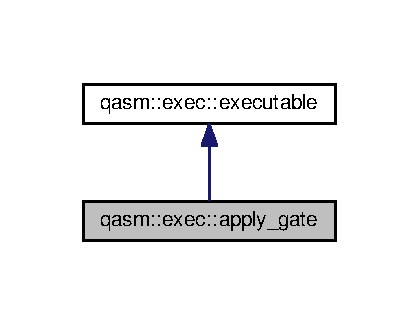
\includegraphics[width=201pt]{classqasm_1_1exec_1_1apply__gate__inherit__graph}
\end{center}
\end{figure}


Collaboration diagram for qasm\+:\+:exec\+:\+:apply\+\_\+gate\+:\nopagebreak
\begin{figure}[H]
\begin{center}
\leavevmode
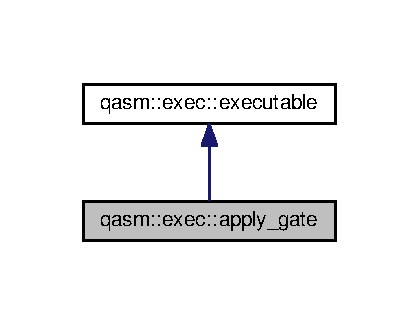
\includegraphics[width=201pt]{classqasm_1_1exec_1_1apply__gate__coll__graph}
\end{center}
\end{figure}
\subsection*{Public Member Functions}
\begin{DoxyCompactItemize}
\item 
\hyperlink{classqasm_1_1exec_1_1apply__gate_a0e7787396ea68b95df1e6a395cd21f2e}{apply\+\_\+gate} (string \hyperlink{classqasm_1_1exec_1_1apply__gate_a2b5eea4ddab7101ab5353ecd160e0d30}{name})
\item 
virtual void \hyperlink{classqasm_1_1exec_1_1apply__gate_a4ab94a7feee1830b4be52a487e9cdef5}{invoke\+\_\+rootprogram} (\hyperlink{classqasm_1_1runtime_1_1environment}{runtime\+::environment} \&env)
\end{DoxyCompactItemize}
\subsection*{Public Attributes}
\begin{DoxyCompactItemize}
\item 
std\+::string \hyperlink{classqasm_1_1exec_1_1apply__gate_a2b5eea4ddab7101ab5353ecd160e0d30}{name}
\item 
std\+::vector$<$ std\+::string $>$ \hyperlink{classqasm_1_1exec_1_1apply__gate_afa925dd76a3c14f5a3739bbd1ab20258}{param\+\_\+names}
\item 
std\+::vector$<$ u64 $>$ \hyperlink{classqasm_1_1exec_1_1apply__gate_a45e00e882c9241a288dae90ae0faa77f}{param\+\_\+indecies}
\end{DoxyCompactItemize}


\subsection{Detailed Description}
Instruction to apply a gate to a register 

\subsection{Constructor \& Destructor Documentation}
\index{qasm\+::exec\+::apply\+\_\+gate@{qasm\+::exec\+::apply\+\_\+gate}!apply\+\_\+gate@{apply\+\_\+gate}}
\index{apply\+\_\+gate@{apply\+\_\+gate}!qasm\+::exec\+::apply\+\_\+gate@{qasm\+::exec\+::apply\+\_\+gate}}
\subsubsection[{\texorpdfstring{apply\+\_\+gate(string name)}{apply_gate(string name)}}]{\setlength{\rightskip}{0pt plus 5cm}qasm\+::exec\+::apply\+\_\+gate\+::apply\+\_\+gate (
\begin{DoxyParamCaption}
\item[{string}]{name}
\end{DoxyParamCaption}
)\hspace{0.3cm}{\ttfamily [inline]}}\hypertarget{classqasm_1_1exec_1_1apply__gate_a0e7787396ea68b95df1e6a395cd21f2e}{}\label{classqasm_1_1exec_1_1apply__gate_a0e7787396ea68b95df1e6a395cd21f2e}


\subsection{Member Function Documentation}
\index{qasm\+::exec\+::apply\+\_\+gate@{qasm\+::exec\+::apply\+\_\+gate}!invoke\+\_\+rootprogram@{invoke\+\_\+rootprogram}}
\index{invoke\+\_\+rootprogram@{invoke\+\_\+rootprogram}!qasm\+::exec\+::apply\+\_\+gate@{qasm\+::exec\+::apply\+\_\+gate}}
\subsubsection[{\texorpdfstring{invoke\+\_\+rootprogram(runtime\+::environment \&env)}{invoke_rootprogram(runtime::environment &env)}}]{\setlength{\rightskip}{0pt plus 5cm}virtual void qasm\+::exec\+::apply\+\_\+gate\+::invoke\+\_\+rootprogram (
\begin{DoxyParamCaption}
\item[{{\bf runtime\+::environment} \&}]{env}
\end{DoxyParamCaption}
)\hspace{0.3cm}{\ttfamily [inline]}, {\ttfamily [virtual]}}\hypertarget{classqasm_1_1exec_1_1apply__gate_a4ab94a7feee1830b4be52a487e9cdef5}{}\label{classqasm_1_1exec_1_1apply__gate_a4ab94a7feee1830b4be52a487e9cdef5}
Run instruction\textquotesingle{}s primary operation 

Reimplemented from \hyperlink{classqasm_1_1exec_1_1executable_ad07f864a889edb0777ebbb1bc1628121}{qasm\+::exec\+::executable}.



\subsection{Member Data Documentation}
\index{qasm\+::exec\+::apply\+\_\+gate@{qasm\+::exec\+::apply\+\_\+gate}!name@{name}}
\index{name@{name}!qasm\+::exec\+::apply\+\_\+gate@{qasm\+::exec\+::apply\+\_\+gate}}
\subsubsection[{\texorpdfstring{name}{name}}]{\setlength{\rightskip}{0pt plus 5cm}std\+::string qasm\+::exec\+::apply\+\_\+gate\+::name}\hypertarget{classqasm_1_1exec_1_1apply__gate_a2b5eea4ddab7101ab5353ecd160e0d30}{}\label{classqasm_1_1exec_1_1apply__gate_a2b5eea4ddab7101ab5353ecd160e0d30}
Name of gate to apply \index{qasm\+::exec\+::apply\+\_\+gate@{qasm\+::exec\+::apply\+\_\+gate}!param\+\_\+indecies@{param\+\_\+indecies}}
\index{param\+\_\+indecies@{param\+\_\+indecies}!qasm\+::exec\+::apply\+\_\+gate@{qasm\+::exec\+::apply\+\_\+gate}}
\subsubsection[{\texorpdfstring{param\+\_\+indecies}{param_indecies}}]{\setlength{\rightskip}{0pt plus 5cm}std\+::vector$<$u64$>$ qasm\+::exec\+::apply\+\_\+gate\+::param\+\_\+indecies}\hypertarget{classqasm_1_1exec_1_1apply__gate_a45e00e882c9241a288dae90ae0faa77f}{}\label{classqasm_1_1exec_1_1apply__gate_a45e00e882c9241a288dae90ae0faa77f}
Index of each register to apply to \index{qasm\+::exec\+::apply\+\_\+gate@{qasm\+::exec\+::apply\+\_\+gate}!param\+\_\+names@{param\+\_\+names}}
\index{param\+\_\+names@{param\+\_\+names}!qasm\+::exec\+::apply\+\_\+gate@{qasm\+::exec\+::apply\+\_\+gate}}
\subsubsection[{\texorpdfstring{param\+\_\+names}{param_names}}]{\setlength{\rightskip}{0pt plus 5cm}std\+::vector$<$std\+::string$>$ qasm\+::exec\+::apply\+\_\+gate\+::param\+\_\+names}\hypertarget{classqasm_1_1exec_1_1apply__gate_afa925dd76a3c14f5a3739bbd1ab20258}{}\label{classqasm_1_1exec_1_1apply__gate_afa925dd76a3c14f5a3739bbd1ab20258}
Name of registers to apply to (should be all the same) 

The documentation for this class was generated from the following file\+:\begin{DoxyCompactItemize}
\item 
src/runtime/\hyperlink{runtime_8hpp}{runtime.\+hpp}\end{DoxyCompactItemize}

\hypertarget{classqasm_1_1exec_1_1apply__subcircuit}{}\section{qasm\+:\+:exec\+:\+:apply\+\_\+subcircuit Class Reference}
\label{classqasm_1_1exec_1_1apply__subcircuit}\index{qasm\+::exec\+::apply\+\_\+subcircuit@{qasm\+::exec\+::apply\+\_\+subcircuit}}


{\ttfamily \#include $<$runtime.\+hpp$>$}



Inheritance diagram for qasm\+:\+:exec\+:\+:apply\+\_\+subcircuit\+:\nopagebreak
\begin{figure}[H]
\begin{center}
\leavevmode
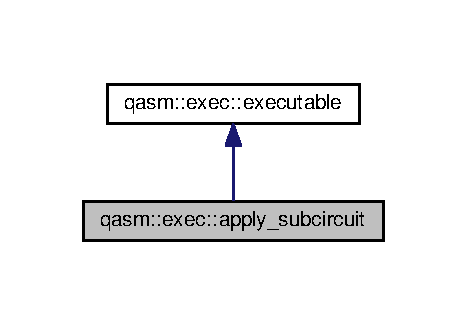
\includegraphics[width=224pt]{classqasm_1_1exec_1_1apply__subcircuit__inherit__graph}
\end{center}
\end{figure}


Collaboration diagram for qasm\+:\+:exec\+:\+:apply\+\_\+subcircuit\+:\nopagebreak
\begin{figure}[H]
\begin{center}
\leavevmode
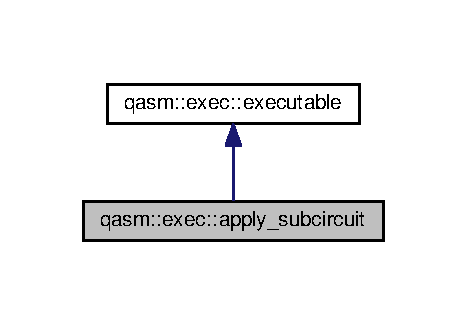
\includegraphics[width=224pt]{classqasm_1_1exec_1_1apply__subcircuit__coll__graph}
\end{center}
\end{figure}
\subsection*{Public Member Functions}
\begin{DoxyCompactItemize}
\item 
\hyperlink{classqasm_1_1exec_1_1apply__subcircuit_ae8196f004b4d61d15a4ae6bad33ce8e5}{apply\+\_\+subcircuit} (string \hyperlink{classqasm_1_1exec_1_1apply__subcircuit_a6bf64c96ecf46285e9d18987a91b37fa}{name})
\end{DoxyCompactItemize}
\subsection*{Public Attributes}
\begin{DoxyCompactItemize}
\item 
std\+::string \hyperlink{classqasm_1_1exec_1_1apply__subcircuit_a6bf64c96ecf46285e9d18987a91b37fa}{name}
\item 
std\+::vector$<$ std\+::string $>$ \hyperlink{classqasm_1_1exec_1_1apply__subcircuit_ac7828e8ae990026dbcf6bb7b5cdc1d9b}{params}
\end{DoxyCompactItemize}


\subsection{Detailed Description}
Instruction to execute a subcircuit program 

\subsection{Constructor \& Destructor Documentation}
\index{qasm\+::exec\+::apply\+\_\+subcircuit@{qasm\+::exec\+::apply\+\_\+subcircuit}!apply\+\_\+subcircuit@{apply\+\_\+subcircuit}}
\index{apply\+\_\+subcircuit@{apply\+\_\+subcircuit}!qasm\+::exec\+::apply\+\_\+subcircuit@{qasm\+::exec\+::apply\+\_\+subcircuit}}
\subsubsection[{\texorpdfstring{apply\+\_\+subcircuit(string name)}{apply_subcircuit(string name)}}]{\setlength{\rightskip}{0pt plus 5cm}qasm\+::exec\+::apply\+\_\+subcircuit\+::apply\+\_\+subcircuit (
\begin{DoxyParamCaption}
\item[{string}]{name}
\end{DoxyParamCaption}
)\hspace{0.3cm}{\ttfamily [inline]}}\hypertarget{classqasm_1_1exec_1_1apply__subcircuit_ae8196f004b4d61d15a4ae6bad33ce8e5}{}\label{classqasm_1_1exec_1_1apply__subcircuit_ae8196f004b4d61d15a4ae6bad33ce8e5}


\subsection{Member Data Documentation}
\index{qasm\+::exec\+::apply\+\_\+subcircuit@{qasm\+::exec\+::apply\+\_\+subcircuit}!name@{name}}
\index{name@{name}!qasm\+::exec\+::apply\+\_\+subcircuit@{qasm\+::exec\+::apply\+\_\+subcircuit}}
\subsubsection[{\texorpdfstring{name}{name}}]{\setlength{\rightskip}{0pt plus 5cm}std\+::string qasm\+::exec\+::apply\+\_\+subcircuit\+::name}\hypertarget{classqasm_1_1exec_1_1apply__subcircuit_a6bf64c96ecf46285e9d18987a91b37fa}{}\label{classqasm_1_1exec_1_1apply__subcircuit_a6bf64c96ecf46285e9d18987a91b37fa}
Name of subcircuit to run \index{qasm\+::exec\+::apply\+\_\+subcircuit@{qasm\+::exec\+::apply\+\_\+subcircuit}!params@{params}}
\index{params@{params}!qasm\+::exec\+::apply\+\_\+subcircuit@{qasm\+::exec\+::apply\+\_\+subcircuit}}
\subsubsection[{\texorpdfstring{params}{params}}]{\setlength{\rightskip}{0pt plus 5cm}std\+::vector$<$std\+::string$>$ qasm\+::exec\+::apply\+\_\+subcircuit\+::params}\hypertarget{classqasm_1_1exec_1_1apply__subcircuit_ac7828e8ae990026dbcf6bb7b5cdc1d9b}{}\label{classqasm_1_1exec_1_1apply__subcircuit_ac7828e8ae990026dbcf6bb7b5cdc1d9b}
Parameters to pass to subcircuit 

The documentation for this class was generated from the following file\+:\begin{DoxyCompactItemize}
\item 
src/runtime/\hyperlink{runtime_8hpp}{runtime.\+hpp}\end{DoxyCompactItemize}

\hypertarget{classqlib_1_1ide_1_1AutoComplete}{}\section{qlib.\+ide.\+Auto\+Complete Class Reference}
\label{classqlib_1_1ide_1_1AutoComplete}\index{qlib.\+ide.\+Auto\+Complete@{qlib.\+ide.\+Auto\+Complete}}


Collaboration diagram for qlib.\+ide.\+Auto\+Complete\+:\nopagebreak
\begin{figure}[H]
\begin{center}
\leavevmode
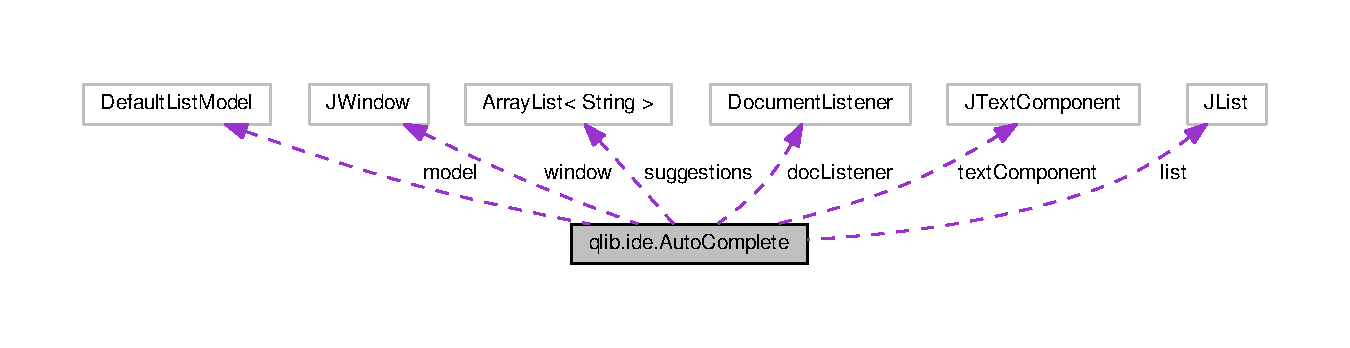
\includegraphics[width=350pt]{classqlib_1_1ide_1_1AutoComplete__coll__graph}
\end{center}
\end{figure}
\subsection*{Public Member Functions}
\begin{DoxyCompactItemize}
\item 
\hyperlink{classqlib_1_1ide_1_1AutoComplete_a30e4dd8e6c36a6ef576641480d4368f7}{Auto\+Complete} (J\+Text\+Component \hyperlink{classqlib_1_1ide_1_1AutoComplete_ab41cb720a8247194d0c4c2cc5fa6aeef}{text\+Component})
\item 
boolean \hyperlink{classqlib_1_1ide_1_1AutoComplete_a6dfe58b003099399cbed40a8082631ff}{is\+Visible} ()
\item 
void \hyperlink{classqlib_1_1ide_1_1AutoComplete_a1b3f11041ae6af9b54e56c19adbbae5c}{add\+Word} (String s)
\item 
void \hyperlink{classqlib_1_1ide_1_1AutoComplete_a8e424fd802e81ab9a816c9b54c8cf364}{remove\+Word} (String s)
\item 
void \hyperlink{classqlib_1_1ide_1_1AutoComplete_aea2eaa12383e22951f5ddef7b9182b07}{set\+Characters\+Until\+Suggestions} (int characters)
\end{DoxyCompactItemize}
\subsection*{Private Member Functions}
\begin{DoxyCompactItemize}
\item 
void \hyperlink{classqlib_1_1ide_1_1AutoComplete_af2b5cb3b8c9557abaed28883288f5f34}{insert\+Suggestion} (Object o)
\item 
void \hyperlink{classqlib_1_1ide_1_1AutoComplete_a9b4c1fc14bdff51a29b3a13622cba025}{show\+Suggestions} ()
\item 
void \hyperlink{classqlib_1_1ide_1_1AutoComplete_a262b15fe050727186b0dc3d22e0d5143}{hide\+Suggestions} ()
\item 
String \hyperlink{classqlib_1_1ide_1_1AutoComplete_acdc8c857e1580998523ee6f50c738a84}{get\+Text} (int start, int length)
\item 
void \hyperlink{classqlib_1_1ide_1_1AutoComplete_a04a7f33c4d243d3d15592c3b0b1b19d4}{check\+For\+And\+Show\+Suggestions} ()
\end{DoxyCompactItemize}
\subsection*{Private Attributes}
\begin{DoxyCompactItemize}
\item 
final J\+Text\+Component \hyperlink{classqlib_1_1ide_1_1AutoComplete_ab41cb720a8247194d0c4c2cc5fa6aeef}{text\+Component}
\item 
final Document\+Listener \hyperlink{classqlib_1_1ide_1_1AutoComplete_a79190bf245b656b279233a982ed4248c}{doc\+Listener}
\item 
final Array\+List$<$ String $>$ \hyperlink{classqlib_1_1ide_1_1AutoComplete_a547307db6247e63b17bad503504dbd22}{suggestions} = new Array\+List$<$String$>$()
\item 
int \hyperlink{classqlib_1_1ide_1_1AutoComplete_ab4de0d96f7b92c3768e1c08fbb47aed5}{letters\+Until\+Shown} = 1
\item 
String \hyperlink{classqlib_1_1ide_1_1AutoComplete_add24423a55cac629e8316c5918a6d954}{typed\+Word}
\item 
int \hyperlink{classqlib_1_1ide_1_1AutoComplete_a7a588e36bc43ffbb782e6f43d89176a2}{start\+Position}
\item 
int \hyperlink{classqlib_1_1ide_1_1AutoComplete_ab737bdeda6e26125bc85ad00f5de14d2}{end\+Position}
\item 
final J\+Window \hyperlink{classqlib_1_1ide_1_1AutoComplete_a858e66824f2ef4066d9987b4206037a2}{window} = new J\+Window()
\item 
J\+List \hyperlink{classqlib_1_1ide_1_1AutoComplete_ab04a22ed940369f199952db2ce1c04f8}{list} = new J\+List()
\item 
Default\+List\+Model \hyperlink{classqlib_1_1ide_1_1AutoComplete_aaaa89916b82f63bd8d7079c84c251e27}{model} = new Default\+List\+Model()
\item 
int \hyperlink{classqlib_1_1ide_1_1AutoComplete_a312cdabc82431a5cc8d73c1884c416a7}{width} = 430
\item 
int \hyperlink{classqlib_1_1ide_1_1AutoComplete_a8ebc95801d3b19aff09123cf8729e2c9}{max\+Height} = 160
\end{DoxyCompactItemize}


\subsection{Detailed Description}
Class for auto complete word suggestions used with J\+Text\+Component \begin{DoxyAuthor}{Author}
chalseth 
\end{DoxyAuthor}


\subsection{Constructor \& Destructor Documentation}
\index{qlib\+::ide\+::\+Auto\+Complete@{qlib\+::ide\+::\+Auto\+Complete}!Auto\+Complete@{Auto\+Complete}}
\index{Auto\+Complete@{Auto\+Complete}!qlib\+::ide\+::\+Auto\+Complete@{qlib\+::ide\+::\+Auto\+Complete}}
\subsubsection[{\texorpdfstring{Auto\+Complete(\+J\+Text\+Component text\+Component)}{AutoComplete(JTextComponent textComponent)}}]{\setlength{\rightskip}{0pt plus 5cm}qlib.\+ide.\+Auto\+Complete.\+Auto\+Complete (
\begin{DoxyParamCaption}
\item[{J\+Text\+Component}]{text\+Component}
\end{DoxyParamCaption}
)\hspace{0.3cm}{\ttfamily [inline]}}\hypertarget{classqlib_1_1ide_1_1AutoComplete_a30e4dd8e6c36a6ef576641480d4368f7}{}\label{classqlib_1_1ide_1_1AutoComplete_a30e4dd8e6c36a6ef576641480d4368f7}
Create an auto complete suggestion dialog for the given text component 
\begin{DoxyParams}{Parameters}
{\em text\+Component} & \\
\hline
\end{DoxyParams}


\subsection{Member Function Documentation}
\index{qlib\+::ide\+::\+Auto\+Complete@{qlib\+::ide\+::\+Auto\+Complete}!add\+Word@{add\+Word}}
\index{add\+Word@{add\+Word}!qlib\+::ide\+::\+Auto\+Complete@{qlib\+::ide\+::\+Auto\+Complete}}
\subsubsection[{\texorpdfstring{add\+Word(\+String s)}{addWord(String s)}}]{\setlength{\rightskip}{0pt plus 5cm}void qlib.\+ide.\+Auto\+Complete.\+add\+Word (
\begin{DoxyParamCaption}
\item[{String}]{s}
\end{DoxyParamCaption}
)\hspace{0.3cm}{\ttfamily [inline]}}\hypertarget{classqlib_1_1ide_1_1AutoComplete_a1b3f11041ae6af9b54e56c19adbbae5c}{}\label{classqlib_1_1ide_1_1AutoComplete_a1b3f11041ae6af9b54e56c19adbbae5c}
Add word to the dictionary 
\begin{DoxyParams}{Parameters}
{\em s} & \\
\hline
\end{DoxyParams}
\index{qlib\+::ide\+::\+Auto\+Complete@{qlib\+::ide\+::\+Auto\+Complete}!check\+For\+And\+Show\+Suggestions@{check\+For\+And\+Show\+Suggestions}}
\index{check\+For\+And\+Show\+Suggestions@{check\+For\+And\+Show\+Suggestions}!qlib\+::ide\+::\+Auto\+Complete@{qlib\+::ide\+::\+Auto\+Complete}}
\subsubsection[{\texorpdfstring{check\+For\+And\+Show\+Suggestions()}{checkForAndShowSuggestions()}}]{\setlength{\rightskip}{0pt plus 5cm}void qlib.\+ide.\+Auto\+Complete.\+check\+For\+And\+Show\+Suggestions (
\begin{DoxyParamCaption}
{}
\end{DoxyParamCaption}
)\hspace{0.3cm}{\ttfamily [inline]}, {\ttfamily [private]}}\hypertarget{classqlib_1_1ide_1_1AutoComplete_a04a7f33c4d243d3d15592c3b0b1b19d4}{}\label{classqlib_1_1ide_1_1AutoComplete_a04a7f33c4d243d3d15592c3b0b1b19d4}
For use auto checking the suggestions as a user types \index{qlib\+::ide\+::\+Auto\+Complete@{qlib\+::ide\+::\+Auto\+Complete}!get\+Text@{get\+Text}}
\index{get\+Text@{get\+Text}!qlib\+::ide\+::\+Auto\+Complete@{qlib\+::ide\+::\+Auto\+Complete}}
\subsubsection[{\texorpdfstring{get\+Text(int start, int length)}{getText(int start, int length)}}]{\setlength{\rightskip}{0pt plus 5cm}String qlib.\+ide.\+Auto\+Complete.\+get\+Text (
\begin{DoxyParamCaption}
\item[{int}]{start, }
\item[{int}]{length}
\end{DoxyParamCaption}
)\hspace{0.3cm}{\ttfamily [inline]}, {\ttfamily [private]}}\hypertarget{classqlib_1_1ide_1_1AutoComplete_acdc8c857e1580998523ee6f50c738a84}{}\label{classqlib_1_1ide_1_1AutoComplete_acdc8c857e1580998523ee6f50c738a84}
Get the text between 2 indexes 
\begin{DoxyParams}{Parameters}
{\em start} & \\
\hline
{\em length} & \\
\hline
\end{DoxyParams}
\begin{DoxyReturn}{Returns}

\end{DoxyReturn}
\index{qlib\+::ide\+::\+Auto\+Complete@{qlib\+::ide\+::\+Auto\+Complete}!hide\+Suggestions@{hide\+Suggestions}}
\index{hide\+Suggestions@{hide\+Suggestions}!qlib\+::ide\+::\+Auto\+Complete@{qlib\+::ide\+::\+Auto\+Complete}}
\subsubsection[{\texorpdfstring{hide\+Suggestions()}{hideSuggestions()}}]{\setlength{\rightskip}{0pt plus 5cm}void qlib.\+ide.\+Auto\+Complete.\+hide\+Suggestions (
\begin{DoxyParamCaption}
{}
\end{DoxyParamCaption}
)\hspace{0.3cm}{\ttfamily [inline]}, {\ttfamily [private]}}\hypertarget{classqlib_1_1ide_1_1AutoComplete_a262b15fe050727186b0dc3d22e0d5143}{}\label{classqlib_1_1ide_1_1AutoComplete_a262b15fe050727186b0dc3d22e0d5143}
Hide the suggestion box \index{qlib\+::ide\+::\+Auto\+Complete@{qlib\+::ide\+::\+Auto\+Complete}!insert\+Suggestion@{insert\+Suggestion}}
\index{insert\+Suggestion@{insert\+Suggestion}!qlib\+::ide\+::\+Auto\+Complete@{qlib\+::ide\+::\+Auto\+Complete}}
\subsubsection[{\texorpdfstring{insert\+Suggestion(\+Object o)}{insertSuggestion(Object o)}}]{\setlength{\rightskip}{0pt plus 5cm}void qlib.\+ide.\+Auto\+Complete.\+insert\+Suggestion (
\begin{DoxyParamCaption}
\item[{Object}]{o}
\end{DoxyParamCaption}
)\hspace{0.3cm}{\ttfamily [inline]}, {\ttfamily [private]}}\hypertarget{classqlib_1_1ide_1_1AutoComplete_af2b5cb3b8c9557abaed28883288f5f34}{}\label{classqlib_1_1ide_1_1AutoComplete_af2b5cb3b8c9557abaed28883288f5f34}
Insert word, replacing the currently typed word 
\begin{DoxyParams}{Parameters}
{\em o} & \\
\hline
\end{DoxyParams}
\index{qlib\+::ide\+::\+Auto\+Complete@{qlib\+::ide\+::\+Auto\+Complete}!is\+Visible@{is\+Visible}}
\index{is\+Visible@{is\+Visible}!qlib\+::ide\+::\+Auto\+Complete@{qlib\+::ide\+::\+Auto\+Complete}}
\subsubsection[{\texorpdfstring{is\+Visible()}{isVisible()}}]{\setlength{\rightskip}{0pt plus 5cm}boolean qlib.\+ide.\+Auto\+Complete.\+is\+Visible (
\begin{DoxyParamCaption}
{}
\end{DoxyParamCaption}
)\hspace{0.3cm}{\ttfamily [inline]}}\hypertarget{classqlib_1_1ide_1_1AutoComplete_a6dfe58b003099399cbed40a8082631ff}{}\label{classqlib_1_1ide_1_1AutoComplete_a6dfe58b003099399cbed40a8082631ff}
Check if the suggestion box is visible \begin{DoxyReturn}{Returns}

\end{DoxyReturn}
\index{qlib\+::ide\+::\+Auto\+Complete@{qlib\+::ide\+::\+Auto\+Complete}!remove\+Word@{remove\+Word}}
\index{remove\+Word@{remove\+Word}!qlib\+::ide\+::\+Auto\+Complete@{qlib\+::ide\+::\+Auto\+Complete}}
\subsubsection[{\texorpdfstring{remove\+Word(\+String s)}{removeWord(String s)}}]{\setlength{\rightskip}{0pt plus 5cm}void qlib.\+ide.\+Auto\+Complete.\+remove\+Word (
\begin{DoxyParamCaption}
\item[{String}]{s}
\end{DoxyParamCaption}
)\hspace{0.3cm}{\ttfamily [inline]}}\hypertarget{classqlib_1_1ide_1_1AutoComplete_a8e424fd802e81ab9a816c9b54c8cf364}{}\label{classqlib_1_1ide_1_1AutoComplete_a8e424fd802e81ab9a816c9b54c8cf364}
Remove word from the dictionary 
\begin{DoxyParams}{Parameters}
{\em s} & \\
\hline
\end{DoxyParams}
\index{qlib\+::ide\+::\+Auto\+Complete@{qlib\+::ide\+::\+Auto\+Complete}!set\+Characters\+Until\+Suggestions@{set\+Characters\+Until\+Suggestions}}
\index{set\+Characters\+Until\+Suggestions@{set\+Characters\+Until\+Suggestions}!qlib\+::ide\+::\+Auto\+Complete@{qlib\+::ide\+::\+Auto\+Complete}}
\subsubsection[{\texorpdfstring{set\+Characters\+Until\+Suggestions(int characters)}{setCharactersUntilSuggestions(int characters)}}]{\setlength{\rightskip}{0pt plus 5cm}void qlib.\+ide.\+Auto\+Complete.\+set\+Characters\+Until\+Suggestions (
\begin{DoxyParamCaption}
\item[{int}]{characters}
\end{DoxyParamCaption}
)\hspace{0.3cm}{\ttfamily [inline]}}\hypertarget{classqlib_1_1ide_1_1AutoComplete_aea2eaa12383e22951f5ddef7b9182b07}{}\label{classqlib_1_1ide_1_1AutoComplete_aea2eaa12383e22951f5ddef7b9182b07}
Set the number of characters until the suggestion box is shown 
\begin{DoxyParams}{Parameters}
{\em characters} & \\
\hline
\end{DoxyParams}
\index{qlib\+::ide\+::\+Auto\+Complete@{qlib\+::ide\+::\+Auto\+Complete}!show\+Suggestions@{show\+Suggestions}}
\index{show\+Suggestions@{show\+Suggestions}!qlib\+::ide\+::\+Auto\+Complete@{qlib\+::ide\+::\+Auto\+Complete}}
\subsubsection[{\texorpdfstring{show\+Suggestions()}{showSuggestions()}}]{\setlength{\rightskip}{0pt plus 5cm}void qlib.\+ide.\+Auto\+Complete.\+show\+Suggestions (
\begin{DoxyParamCaption}
{}
\end{DoxyParamCaption}
)\hspace{0.3cm}{\ttfamily [inline]}, {\ttfamily [private]}}\hypertarget{classqlib_1_1ide_1_1AutoComplete_a9b4c1fc14bdff51a29b3a13622cba025}{}\label{classqlib_1_1ide_1_1AutoComplete_a9b4c1fc14bdff51a29b3a13622cba025}
Show the suggestion box 

\subsection{Member Data Documentation}
\index{qlib\+::ide\+::\+Auto\+Complete@{qlib\+::ide\+::\+Auto\+Complete}!doc\+Listener@{doc\+Listener}}
\index{doc\+Listener@{doc\+Listener}!qlib\+::ide\+::\+Auto\+Complete@{qlib\+::ide\+::\+Auto\+Complete}}
\subsubsection[{\texorpdfstring{doc\+Listener}{docListener}}]{\setlength{\rightskip}{0pt plus 5cm}final Document\+Listener qlib.\+ide.\+Auto\+Complete.\+doc\+Listener\hspace{0.3cm}{\ttfamily [private]}}\hypertarget{classqlib_1_1ide_1_1AutoComplete_a79190bf245b656b279233a982ed4248c}{}\label{classqlib_1_1ide_1_1AutoComplete_a79190bf245b656b279233a982ed4248c}
{\bfseries Initial value\+:}
\begin{DoxyCode}
= \textcolor{keyword}{new} DocumentListener() \{
        @Override
        \textcolor{keyword}{public} \textcolor{keywordtype}{void} insertUpdate(DocumentEvent de) \{
            \hyperlink{classqlib_1_1ide_1_1AutoComplete_a04a7f33c4d243d3d15592c3b0b1b19d4}{checkForAndShowSuggestions}();
        \}

        @Override
        \textcolor{keyword}{public} \textcolor{keywordtype}{void} removeUpdate(DocumentEvent de) \{
            \hyperlink{classqlib_1_1ide_1_1AutoComplete_a04a7f33c4d243d3d15592c3b0b1b19d4}{checkForAndShowSuggestions}();
        \}

        @Override
        \textcolor{keyword}{public} \textcolor{keywordtype}{void} changedUpdate(DocumentEvent de) \{
            \hyperlink{classqlib_1_1ide_1_1AutoComplete_a04a7f33c4d243d3d15592c3b0b1b19d4}{checkForAndShowSuggestions}();
        \}
    \}
\end{DoxyCode}
Document listener for the text\+Component \index{qlib\+::ide\+::\+Auto\+Complete@{qlib\+::ide\+::\+Auto\+Complete}!end\+Position@{end\+Position}}
\index{end\+Position@{end\+Position}!qlib\+::ide\+::\+Auto\+Complete@{qlib\+::ide\+::\+Auto\+Complete}}
\subsubsection[{\texorpdfstring{end\+Position}{endPosition}}]{\setlength{\rightskip}{0pt plus 5cm}int qlib.\+ide.\+Auto\+Complete.\+end\+Position\hspace{0.3cm}{\ttfamily [private]}}\hypertarget{classqlib_1_1ide_1_1AutoComplete_ab737bdeda6e26125bc85ad00f5de14d2}{}\label{classqlib_1_1ide_1_1AutoComplete_ab737bdeda6e26125bc85ad00f5de14d2}
End index of the typed word \index{qlib\+::ide\+::\+Auto\+Complete@{qlib\+::ide\+::\+Auto\+Complete}!letters\+Until\+Shown@{letters\+Until\+Shown}}
\index{letters\+Until\+Shown@{letters\+Until\+Shown}!qlib\+::ide\+::\+Auto\+Complete@{qlib\+::ide\+::\+Auto\+Complete}}
\subsubsection[{\texorpdfstring{letters\+Until\+Shown}{lettersUntilShown}}]{\setlength{\rightskip}{0pt plus 5cm}int qlib.\+ide.\+Auto\+Complete.\+letters\+Until\+Shown = 1\hspace{0.3cm}{\ttfamily [private]}}\hypertarget{classqlib_1_1ide_1_1AutoComplete_ab4de0d96f7b92c3768e1c08fbb47aed5}{}\label{classqlib_1_1ide_1_1AutoComplete_ab4de0d96f7b92c3768e1c08fbb47aed5}
Number of letters until suggestions get shown \index{qlib\+::ide\+::\+Auto\+Complete@{qlib\+::ide\+::\+Auto\+Complete}!list@{list}}
\index{list@{list}!qlib\+::ide\+::\+Auto\+Complete@{qlib\+::ide\+::\+Auto\+Complete}}
\subsubsection[{\texorpdfstring{list}{list}}]{\setlength{\rightskip}{0pt plus 5cm}J\+List qlib.\+ide.\+Auto\+Complete.\+list = new J\+List()\hspace{0.3cm}{\ttfamily [private]}}\hypertarget{classqlib_1_1ide_1_1AutoComplete_ab04a22ed940369f199952db2ce1c04f8}{}\label{classqlib_1_1ide_1_1AutoComplete_ab04a22ed940369f199952db2ce1c04f8}
Reference to the list of suggestions \index{qlib\+::ide\+::\+Auto\+Complete@{qlib\+::ide\+::\+Auto\+Complete}!max\+Height@{max\+Height}}
\index{max\+Height@{max\+Height}!qlib\+::ide\+::\+Auto\+Complete@{qlib\+::ide\+::\+Auto\+Complete}}
\subsubsection[{\texorpdfstring{max\+Height}{maxHeight}}]{\setlength{\rightskip}{0pt plus 5cm}int qlib.\+ide.\+Auto\+Complete.\+max\+Height = 160\hspace{0.3cm}{\ttfamily [private]}}\hypertarget{classqlib_1_1ide_1_1AutoComplete_a8ebc95801d3b19aff09123cf8729e2c9}{}\label{classqlib_1_1ide_1_1AutoComplete_a8ebc95801d3b19aff09123cf8729e2c9}
Maximum height of the suggestion window \index{qlib\+::ide\+::\+Auto\+Complete@{qlib\+::ide\+::\+Auto\+Complete}!model@{model}}
\index{model@{model}!qlib\+::ide\+::\+Auto\+Complete@{qlib\+::ide\+::\+Auto\+Complete}}
\subsubsection[{\texorpdfstring{model}{model}}]{\setlength{\rightskip}{0pt plus 5cm}Default\+List\+Model qlib.\+ide.\+Auto\+Complete.\+model = new Default\+List\+Model()\hspace{0.3cm}{\ttfamily [private]}}\hypertarget{classqlib_1_1ide_1_1AutoComplete_aaaa89916b82f63bd8d7079c84c251e27}{}\label{classqlib_1_1ide_1_1AutoComplete_aaaa89916b82f63bd8d7079c84c251e27}
Reference to the list\textquotesingle{}s data model \index{qlib\+::ide\+::\+Auto\+Complete@{qlib\+::ide\+::\+Auto\+Complete}!start\+Position@{start\+Position}}
\index{start\+Position@{start\+Position}!qlib\+::ide\+::\+Auto\+Complete@{qlib\+::ide\+::\+Auto\+Complete}}
\subsubsection[{\texorpdfstring{start\+Position}{startPosition}}]{\setlength{\rightskip}{0pt plus 5cm}int qlib.\+ide.\+Auto\+Complete.\+start\+Position\hspace{0.3cm}{\ttfamily [private]}}\hypertarget{classqlib_1_1ide_1_1AutoComplete_a7a588e36bc43ffbb782e6f43d89176a2}{}\label{classqlib_1_1ide_1_1AutoComplete_a7a588e36bc43ffbb782e6f43d89176a2}
Start index of the typed word \index{qlib\+::ide\+::\+Auto\+Complete@{qlib\+::ide\+::\+Auto\+Complete}!suggestions@{suggestions}}
\index{suggestions@{suggestions}!qlib\+::ide\+::\+Auto\+Complete@{qlib\+::ide\+::\+Auto\+Complete}}
\subsubsection[{\texorpdfstring{suggestions}{suggestions}}]{\setlength{\rightskip}{0pt plus 5cm}final Array\+List$<$String$>$ qlib.\+ide.\+Auto\+Complete.\+suggestions = new Array\+List$<$String$>$()\hspace{0.3cm}{\ttfamily [private]}}\hypertarget{classqlib_1_1ide_1_1AutoComplete_a547307db6247e63b17bad503504dbd22}{}\label{classqlib_1_1ide_1_1AutoComplete_a547307db6247e63b17bad503504dbd22}
List of words to suggest \index{qlib\+::ide\+::\+Auto\+Complete@{qlib\+::ide\+::\+Auto\+Complete}!text\+Component@{text\+Component}}
\index{text\+Component@{text\+Component}!qlib\+::ide\+::\+Auto\+Complete@{qlib\+::ide\+::\+Auto\+Complete}}
\subsubsection[{\texorpdfstring{text\+Component}{textComponent}}]{\setlength{\rightskip}{0pt plus 5cm}final J\+Text\+Component qlib.\+ide.\+Auto\+Complete.\+text\+Component\hspace{0.3cm}{\ttfamily [private]}}\hypertarget{classqlib_1_1ide_1_1AutoComplete_ab41cb720a8247194d0c4c2cc5fa6aeef}{}\label{classqlib_1_1ide_1_1AutoComplete_ab41cb720a8247194d0c4c2cc5fa6aeef}
Parent text component \index{qlib\+::ide\+::\+Auto\+Complete@{qlib\+::ide\+::\+Auto\+Complete}!typed\+Word@{typed\+Word}}
\index{typed\+Word@{typed\+Word}!qlib\+::ide\+::\+Auto\+Complete@{qlib\+::ide\+::\+Auto\+Complete}}
\subsubsection[{\texorpdfstring{typed\+Word}{typedWord}}]{\setlength{\rightskip}{0pt plus 5cm}String qlib.\+ide.\+Auto\+Complete.\+typed\+Word\hspace{0.3cm}{\ttfamily [private]}}\hypertarget{classqlib_1_1ide_1_1AutoComplete_add24423a55cac629e8316c5918a6d954}{}\label{classqlib_1_1ide_1_1AutoComplete_add24423a55cac629e8316c5918a6d954}
The currently typed word \index{qlib\+::ide\+::\+Auto\+Complete@{qlib\+::ide\+::\+Auto\+Complete}!width@{width}}
\index{width@{width}!qlib\+::ide\+::\+Auto\+Complete@{qlib\+::ide\+::\+Auto\+Complete}}
\subsubsection[{\texorpdfstring{width}{width}}]{\setlength{\rightskip}{0pt plus 5cm}int qlib.\+ide.\+Auto\+Complete.\+width = 430\hspace{0.3cm}{\ttfamily [private]}}\hypertarget{classqlib_1_1ide_1_1AutoComplete_a312cdabc82431a5cc8d73c1884c416a7}{}\label{classqlib_1_1ide_1_1AutoComplete_a312cdabc82431a5cc8d73c1884c416a7}
Width of suggestion window \index{qlib\+::ide\+::\+Auto\+Complete@{qlib\+::ide\+::\+Auto\+Complete}!window@{window}}
\index{window@{window}!qlib\+::ide\+::\+Auto\+Complete@{qlib\+::ide\+::\+Auto\+Complete}}
\subsubsection[{\texorpdfstring{window}{window}}]{\setlength{\rightskip}{0pt plus 5cm}final J\+Window qlib.\+ide.\+Auto\+Complete.\+window = new J\+Window()\hspace{0.3cm}{\ttfamily [private]}}\hypertarget{classqlib_1_1ide_1_1AutoComplete_a858e66824f2ef4066d9987b4206037a2}{}\label{classqlib_1_1ide_1_1AutoComplete_a858e66824f2ef4066d9987b4206037a2}
Reference to the suggestion window 

The documentation for this class was generated from the following file\+:\begin{DoxyCompactItemize}
\item 
src/ide/src/qlib/ide/\hyperlink{AutoComplete_8java}{Auto\+Complete.\+java}\end{DoxyCompactItemize}

\hypertarget{interfaceqlib_1_1ide_1_1CodeEditor_1_1ChangeListener}{}\section{qlib.\+ide.\+Code\+Editor.\+Change\+Listener Interface Reference}
\label{interfaceqlib_1_1ide_1_1CodeEditor_1_1ChangeListener}\index{qlib.\+ide.\+Code\+Editor.\+Change\+Listener@{qlib.\+ide.\+Code\+Editor.\+Change\+Listener}}
\subsection*{Public Member Functions}
\begin{DoxyCompactItemize}
\item 
void \hyperlink{interfaceqlib_1_1ide_1_1CodeEditor_1_1ChangeListener_a4eb57d86f7a6f23c781ebb1d1cd99ce6}{invoke} (String change)
\end{DoxyCompactItemize}


\subsection{Detailed Description}
Internal interface for listeners 

\subsection{Member Function Documentation}
\index{qlib\+::ide\+::\+Code\+Editor\+::\+Change\+Listener@{qlib\+::ide\+::\+Code\+Editor\+::\+Change\+Listener}!invoke@{invoke}}
\index{invoke@{invoke}!qlib\+::ide\+::\+Code\+Editor\+::\+Change\+Listener@{qlib\+::ide\+::\+Code\+Editor\+::\+Change\+Listener}}
\subsubsection[{\texorpdfstring{invoke(\+String change)}{invoke(String change)}}]{\setlength{\rightskip}{0pt plus 5cm}void qlib.\+ide.\+Code\+Editor.\+Change\+Listener.\+invoke (
\begin{DoxyParamCaption}
\item[{String}]{change}
\end{DoxyParamCaption}
)}\hypertarget{interfaceqlib_1_1ide_1_1CodeEditor_1_1ChangeListener_a4eb57d86f7a6f23c781ebb1d1cd99ce6}{}\label{interfaceqlib_1_1ide_1_1CodeEditor_1_1ChangeListener_a4eb57d86f7a6f23c781ebb1d1cd99ce6}


The documentation for this interface was generated from the following file\+:\begin{DoxyCompactItemize}
\item 
src/ide/src/qlib/ide/\hyperlink{CodeEditor_8java}{Code\+Editor.\+java}\end{DoxyCompactItemize}

\hypertarget{classparser_1_1choice}{}\section{parser\+:\+:choice Class Reference}
\label{classparser_1_1choice}\index{parser\+::choice@{parser\+::choice}}


{\ttfamily \#include $<$parser.\+hpp$>$}



Inheritance diagram for parser\+:\+:choice\+:
\nopagebreak
\begin{figure}[H]
\begin{center}
\leavevmode
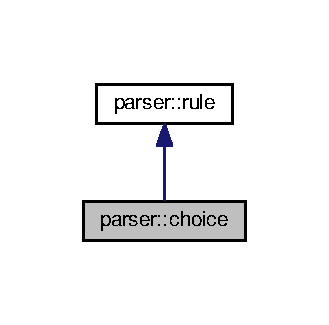
\includegraphics[width=158pt]{classparser_1_1choice__inherit__graph}
\end{center}
\end{figure}


Collaboration diagram for parser\+:\+:choice\+:
\nopagebreak
\begin{figure}[H]
\begin{center}
\leavevmode
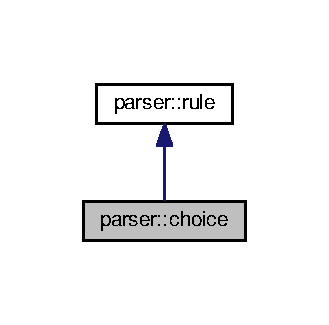
\includegraphics[width=158pt]{classparser_1_1choice__coll__graph}
\end{center}
\end{figure}
\subsection*{Public Member Functions}
\begin{DoxyCompactItemize}
\item 
\hyperlink{classparser_1_1choice_ae9e624b9260ed9006741d6870ea334e4}{choice} (\hyperlink{namespaceparser_a85b2df48287fddaca144a5f6c01b4761}{ruleptr} first, \hyperlink{namespaceparser_a85b2df48287fddaca144a5f6c01b4761}{ruleptr} second)
\item 
\hyperlink{classparser_1_1choice_ad6fe3cd8e19171e387c8ff34e1291f83}{$\sim$choice} ()
\item 
bool \hyperlink{classparser_1_1choice_a76d73bd6b3adb0c8a062b46a4d49cd11}{try\+Parse} (\hyperlink{classparser_1_1tokenqueue}{tokenqueue} \&queue, \hyperlink{structparser_1_1parsetree}{parsetree} $\ast$ref)
\end{DoxyCompactItemize}
\subsection*{Private Attributes}
\begin{DoxyCompactItemize}
\item 
\hyperlink{namespaceparser_a85b2df48287fddaca144a5f6c01b4761}{ruleptr} \hyperlink{classparser_1_1choice_a7ddb22bce6c8446a35a6fbc9ceaaf962}{left}
\item 
\hyperlink{namespaceparser_a85b2df48287fddaca144a5f6c01b4761}{ruleptr} \hyperlink{classparser_1_1choice_a5cd2aac2dea54c11da1495cacd00db10}{right}
\end{DoxyCompactItemize}


\subsection{Detailed Description}
Class representing parsing elements that are either one thing exclusive or another 

\subsection{Constructor \& Destructor Documentation}
\index{parser\+::choice@{parser\+::choice}!choice@{choice}}
\index{choice@{choice}!parser\+::choice@{parser\+::choice}}
\subsubsection[{\texorpdfstring{choice(ruleptr first, ruleptr second)}{choice(ruleptr first, ruleptr second)}}]{\setlength{\rightskip}{0pt plus 5cm}parser\+::choice\+::choice (
\begin{DoxyParamCaption}
\item[{{\bf ruleptr}}]{first, }
\item[{{\bf ruleptr}}]{second}
\end{DoxyParamCaption}
)\hspace{0.3cm}{\ttfamily [inline]}}\hypertarget{classparser_1_1choice_ae9e624b9260ed9006741d6870ea334e4}{}\label{classparser_1_1choice_ae9e624b9260ed9006741d6870ea334e4}
\index{parser\+::choice@{parser\+::choice}!````~choice@{$\sim$choice}}
\index{````~choice@{$\sim$choice}!parser\+::choice@{parser\+::choice}}
\subsubsection[{\texorpdfstring{$\sim$choice()}{~choice()}}]{\setlength{\rightskip}{0pt plus 5cm}parser\+::choice\+::$\sim$choice (
\begin{DoxyParamCaption}
{}
\end{DoxyParamCaption}
)\hspace{0.3cm}{\ttfamily [inline]}}\hypertarget{classparser_1_1choice_ad6fe3cd8e19171e387c8ff34e1291f83}{}\label{classparser_1_1choice_ad6fe3cd8e19171e387c8ff34e1291f83}


\subsection{Member Function Documentation}
\index{parser\+::choice@{parser\+::choice}!try\+Parse@{try\+Parse}}
\index{try\+Parse@{try\+Parse}!parser\+::choice@{parser\+::choice}}
\subsubsection[{\texorpdfstring{try\+Parse(tokenqueue \&queue, parsetree $\ast$ref)}{tryParse(tokenqueue &queue, parsetree *ref)}}]{\setlength{\rightskip}{0pt plus 5cm}bool parser\+::choice\+::try\+Parse (
\begin{DoxyParamCaption}
\item[{{\bf tokenqueue} \&}]{queue, }
\item[{{\bf parsetree} $\ast$}]{ref}
\end{DoxyParamCaption}
)\hspace{0.3cm}{\ttfamily [inline]}, {\ttfamily [virtual]}}\hypertarget{classparser_1_1choice_a76d73bd6b3adb0c8a062b46a4d49cd11}{}\label{classparser_1_1choice_a76d73bd6b3adb0c8a062b46a4d49cd11}
Virtual function to parse an input tokenqueue into a parse tree Returns true if parsing successful and sets the value under the parsetree pointer 

Reimplemented from \hyperlink{classparser_1_1rule_a60ccfb91ea4fe7def5ec2a15bb97c5ec}{parser\+::rule}.



\subsection{Member Data Documentation}
\index{parser\+::choice@{parser\+::choice}!left@{left}}
\index{left@{left}!parser\+::choice@{parser\+::choice}}
\subsubsection[{\texorpdfstring{left}{left}}]{\setlength{\rightskip}{0pt plus 5cm}{\bf ruleptr} parser\+::choice\+::left\hspace{0.3cm}{\ttfamily [private]}}\hypertarget{classparser_1_1choice_a7ddb22bce6c8446a35a6fbc9ceaaf962}{}\label{classparser_1_1choice_a7ddb22bce6c8446a35a6fbc9ceaaf962}
\index{parser\+::choice@{parser\+::choice}!right@{right}}
\index{right@{right}!parser\+::choice@{parser\+::choice}}
\subsubsection[{\texorpdfstring{right}{right}}]{\setlength{\rightskip}{0pt plus 5cm}{\bf ruleptr} parser\+::choice\+::right\hspace{0.3cm}{\ttfamily [private]}}\hypertarget{classparser_1_1choice_a5cd2aac2dea54c11da1495cacd00db10}{}\label{classparser_1_1choice_a5cd2aac2dea54c11da1495cacd00db10}


The documentation for this class was generated from the following file\+:\begin{DoxyCompactItemize}
\item 
src/runtime/\hyperlink{parser_8hpp}{parser.\+hpp}\end{DoxyCompactItemize}

\hypertarget{classqlib_1_1ide_1_1CodeEditor}{}\section{qlib.\+ide.\+Code\+Editor Class Reference}
\label{classqlib_1_1ide_1_1CodeEditor}\index{qlib.\+ide.\+Code\+Editor@{qlib.\+ide.\+Code\+Editor}}


Inheritance diagram for qlib.\+ide.\+Code\+Editor\+:\nopagebreak
\begin{figure}[H]
\begin{center}
\leavevmode
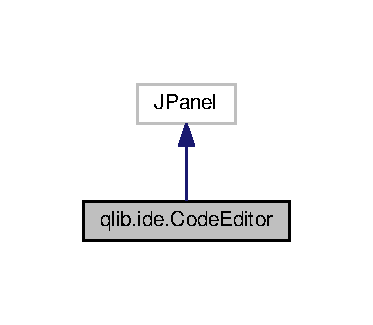
\includegraphics[width=179pt]{classqlib_1_1ide_1_1CodeEditor__inherit__graph}
\end{center}
\end{figure}


Collaboration diagram for qlib.\+ide.\+Code\+Editor\+:\nopagebreak
\begin{figure}[H]
\begin{center}
\leavevmode
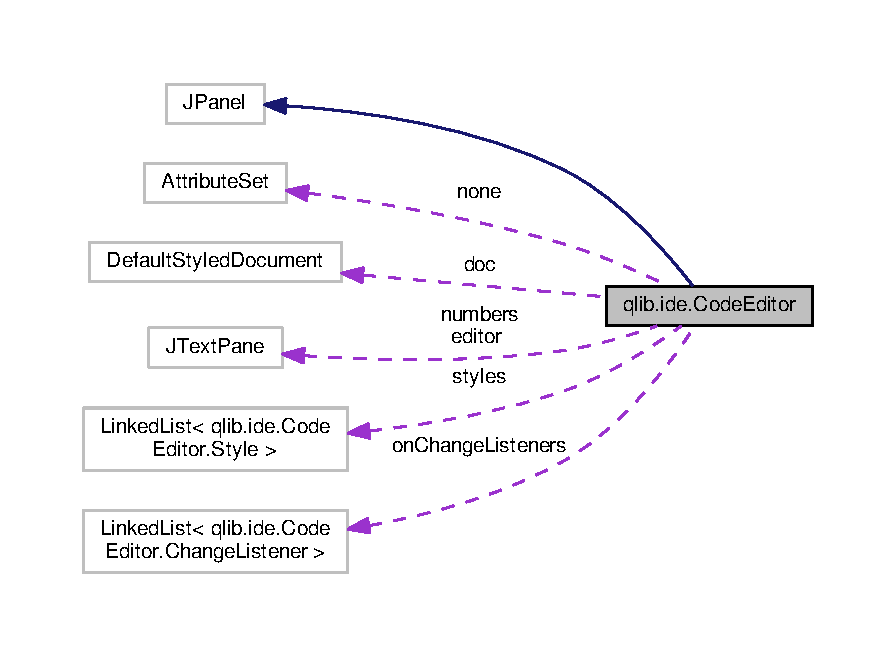
\includegraphics[width=350pt]{classqlib_1_1ide_1_1CodeEditor__coll__graph}
\end{center}
\end{figure}
\subsection*{Classes}
\begin{DoxyCompactItemize}
\item 
interface \hyperlink{interfaceqlib_1_1ide_1_1CodeEditor_1_1ChangeListener}{Change\+Listener}
\item 
class \hyperlink{classqlib_1_1ide_1_1CodeEditor_1_1Style}{Style}
\end{DoxyCompactItemize}
\subsection*{Public Member Functions}
\begin{DoxyCompactItemize}
\item 
\hyperlink{classqlib_1_1ide_1_1CodeEditor_a9f3e1be7ea989d2011bf7d419341405c}{Code\+Editor} ()
\item 
void \hyperlink{classqlib_1_1ide_1_1CodeEditor_a89f62319ae0b01df34fa6ad8f06ddb10}{add\+Change\+Listener} (\hyperlink{interfaceqlib_1_1ide_1_1CodeEditor_1_1ChangeListener}{Change\+Listener} listener)
\item 
void \hyperlink{classqlib_1_1ide_1_1CodeEditor_ab6e32fe9c4f6535ee81fe69d4a77c8f2}{remove\+Change\+Listener} (\hyperlink{interfaceqlib_1_1ide_1_1CodeEditor_1_1ChangeListener}{Change\+Listener} listener)
\item 
void \hyperlink{classqlib_1_1ide_1_1CodeEditor_aabec5fb27bf75e4bb805240dc22c9875}{set\+Background\+Colour} (Color c)
\item 
void \hyperlink{classqlib_1_1ide_1_1CodeEditor_ae1b405cb3544e1869f229e0dbc1a4b0a}{set\+Font\+Colour} (Color c)
\item 
void \hyperlink{classqlib_1_1ide_1_1CodeEditor_a8686347c695b958ea8a5e8737cc59a1f}{set\+Text} (String text)
\item 
String \hyperlink{classqlib_1_1ide_1_1CodeEditor_a7cf3ac3837b11ee6494d45bb7e3d2435}{get\+Text} ()
\item 
void \hyperlink{classqlib_1_1ide_1_1CodeEditor_a65a9670ed0303c4acdaa53b45cc8b5d8}{set\+Font} (Font font)
\item 
void \hyperlink{classqlib_1_1ide_1_1CodeEditor_a5a8026e92f259481f31e26dcbab0e5e2}{add\+Style} (String regex, Color text)
\item 
void \hyperlink{classqlib_1_1ide_1_1CodeEditor_a50cf32315b6cb4d3358a2d00adbae74a}{add\+Style} (String regex, Color text, Color background)
\item 
J\+Text\+Pane \hyperlink{classqlib_1_1ide_1_1CodeEditor_a15327f7a8960ee54f65e4aca0b8e0c69}{get\+Editor} ()
\end{DoxyCompactItemize}
\subsection*{Private Member Functions}
\begin{DoxyCompactItemize}
\item 
void \hyperlink{classqlib_1_1ide_1_1CodeEditor_accee26f5cf7da53ffda849ab6d4741e0}{update\+Numbering} ()
\item 
void \hyperlink{classqlib_1_1ide_1_1CodeEditor_a2fccea5703e28988470c1e4634316ac8}{style} (Default\+Styled\+Document \hyperlink{classqlib_1_1ide_1_1CodeEditor_a89cfdfd40de46ae17636669521f7c7e2}{doc})
\end{DoxyCompactItemize}
\subsection*{Private Attributes}
\begin{DoxyCompactItemize}
\item 
J\+Text\+Pane \hyperlink{classqlib_1_1ide_1_1CodeEditor_a7890793e4b90ebe797bb5e368e72e721}{editor}
\item 
J\+Text\+Pane \hyperlink{classqlib_1_1ide_1_1CodeEditor_ad9b88b89dc797c2eb6511cb5026b30da}{numbers}
\item 
Default\+Styled\+Document \hyperlink{classqlib_1_1ide_1_1CodeEditor_a89cfdfd40de46ae17636669521f7c7e2}{doc}
\item 
Linked\+List$<$ \hyperlink{classqlib_1_1ide_1_1CodeEditor_1_1Style}{Style} $>$ \hyperlink{classqlib_1_1ide_1_1CodeEditor_a126eb2c62a3df4b9f9ce29685f7a474d}{styles} = new Linked\+List$<$\hyperlink{classqlib_1_1ide_1_1CodeEditor_1_1Style}{Style}$>$()
\item 
Attribute\+Set \hyperlink{classqlib_1_1ide_1_1CodeEditor_a108318be527559a6a6fdc044ce91f379}{none}
\item 
Linked\+List$<$ \hyperlink{interfaceqlib_1_1ide_1_1CodeEditor_1_1ChangeListener}{Change\+Listener} $>$ \hyperlink{classqlib_1_1ide_1_1CodeEditor_abbe985cdd77e9feb1818773c377257fb}{on\+Change\+Listeners} = new Linked\+List$<$\hyperlink{interfaceqlib_1_1ide_1_1CodeEditor_1_1ChangeListener}{Change\+Listener}$>$()
\end{DoxyCompactItemize}


\subsection{Detailed Description}
Class representing a code editor with line numbering and syntax highlighting \begin{DoxyAuthor}{Author}
Colin Halseth 
\end{DoxyAuthor}


\subsection{Constructor \& Destructor Documentation}
\index{qlib\+::ide\+::\+Code\+Editor@{qlib\+::ide\+::\+Code\+Editor}!Code\+Editor@{Code\+Editor}}
\index{Code\+Editor@{Code\+Editor}!qlib\+::ide\+::\+Code\+Editor@{qlib\+::ide\+::\+Code\+Editor}}
\subsubsection[{\texorpdfstring{Code\+Editor()}{CodeEditor()}}]{\setlength{\rightskip}{0pt plus 5cm}qlib.\+ide.\+Code\+Editor.\+Code\+Editor (
\begin{DoxyParamCaption}
{}
\end{DoxyParamCaption}
)\hspace{0.3cm}{\ttfamily [inline]}}\hypertarget{classqlib_1_1ide_1_1CodeEditor_a9f3e1be7ea989d2011bf7d419341405c}{}\label{classqlib_1_1ide_1_1CodeEditor_a9f3e1be7ea989d2011bf7d419341405c}
Create a new code editor 

\subsection{Member Function Documentation}
\index{qlib\+::ide\+::\+Code\+Editor@{qlib\+::ide\+::\+Code\+Editor}!add\+Change\+Listener@{add\+Change\+Listener}}
\index{add\+Change\+Listener@{add\+Change\+Listener}!qlib\+::ide\+::\+Code\+Editor@{qlib\+::ide\+::\+Code\+Editor}}
\subsubsection[{\texorpdfstring{add\+Change\+Listener(\+Change\+Listener listener)}{addChangeListener(ChangeListener listener)}}]{\setlength{\rightskip}{0pt plus 5cm}void qlib.\+ide.\+Code\+Editor.\+add\+Change\+Listener (
\begin{DoxyParamCaption}
\item[{{\bf Change\+Listener}}]{listener}
\end{DoxyParamCaption}
)\hspace{0.3cm}{\ttfamily [inline]}}\hypertarget{classqlib_1_1ide_1_1CodeEditor_a89f62319ae0b01df34fa6ad8f06ddb10}{}\label{classqlib_1_1ide_1_1CodeEditor_a89f62319ae0b01df34fa6ad8f06ddb10}
Add a change listener 
\begin{DoxyParams}{Parameters}
{\em listener} & \\
\hline
\end{DoxyParams}
\index{qlib\+::ide\+::\+Code\+Editor@{qlib\+::ide\+::\+Code\+Editor}!add\+Style@{add\+Style}}
\index{add\+Style@{add\+Style}!qlib\+::ide\+::\+Code\+Editor@{qlib\+::ide\+::\+Code\+Editor}}
\subsubsection[{\texorpdfstring{add\+Style(\+String regex, Color text)}{addStyle(String regex, Color text)}}]{\setlength{\rightskip}{0pt plus 5cm}void qlib.\+ide.\+Code\+Editor.\+add\+Style (
\begin{DoxyParamCaption}
\item[{String}]{regex, }
\item[{Color}]{text}
\end{DoxyParamCaption}
)\hspace{0.3cm}{\ttfamily [inline]}}\hypertarget{classqlib_1_1ide_1_1CodeEditor_a5a8026e92f259481f31e26dcbab0e5e2}{}\label{classqlib_1_1ide_1_1CodeEditor_a5a8026e92f259481f31e26dcbab0e5e2}
Add style for regex 
\begin{DoxyParams}{Parameters}
{\em regex} & \\
\hline
{\em text} & \\
\hline
\end{DoxyParams}
\index{qlib\+::ide\+::\+Code\+Editor@{qlib\+::ide\+::\+Code\+Editor}!add\+Style@{add\+Style}}
\index{add\+Style@{add\+Style}!qlib\+::ide\+::\+Code\+Editor@{qlib\+::ide\+::\+Code\+Editor}}
\subsubsection[{\texorpdfstring{add\+Style(\+String regex, Color text, Color background)}{addStyle(String regex, Color text, Color background)}}]{\setlength{\rightskip}{0pt plus 5cm}void qlib.\+ide.\+Code\+Editor.\+add\+Style (
\begin{DoxyParamCaption}
\item[{String}]{regex, }
\item[{Color}]{text, }
\item[{Color}]{background}
\end{DoxyParamCaption}
)\hspace{0.3cm}{\ttfamily [inline]}}\hypertarget{classqlib_1_1ide_1_1CodeEditor_a50cf32315b6cb4d3358a2d00adbae74a}{}\label{classqlib_1_1ide_1_1CodeEditor_a50cf32315b6cb4d3358a2d00adbae74a}
Add style for regex 
\begin{DoxyParams}{Parameters}
{\em regex} & \\
\hline
{\em text} & \\
\hline
{\em background} & \\
\hline
\end{DoxyParams}
\index{qlib\+::ide\+::\+Code\+Editor@{qlib\+::ide\+::\+Code\+Editor}!get\+Editor@{get\+Editor}}
\index{get\+Editor@{get\+Editor}!qlib\+::ide\+::\+Code\+Editor@{qlib\+::ide\+::\+Code\+Editor}}
\subsubsection[{\texorpdfstring{get\+Editor()}{getEditor()}}]{\setlength{\rightskip}{0pt plus 5cm}J\+Text\+Pane qlib.\+ide.\+Code\+Editor.\+get\+Editor (
\begin{DoxyParamCaption}
{}
\end{DoxyParamCaption}
)\hspace{0.3cm}{\ttfamily [inline]}}\hypertarget{classqlib_1_1ide_1_1CodeEditor_a15327f7a8960ee54f65e4aca0b8e0c69}{}\label{classqlib_1_1ide_1_1CodeEditor_a15327f7a8960ee54f65e4aca0b8e0c69}
Get the internal editor panel \begin{DoxyReturn}{Returns}
J\+Text\+Pane 
\end{DoxyReturn}
\index{qlib\+::ide\+::\+Code\+Editor@{qlib\+::ide\+::\+Code\+Editor}!get\+Text@{get\+Text}}
\index{get\+Text@{get\+Text}!qlib\+::ide\+::\+Code\+Editor@{qlib\+::ide\+::\+Code\+Editor}}
\subsubsection[{\texorpdfstring{get\+Text()}{getText()}}]{\setlength{\rightskip}{0pt plus 5cm}String qlib.\+ide.\+Code\+Editor.\+get\+Text (
\begin{DoxyParamCaption}
{}
\end{DoxyParamCaption}
)\hspace{0.3cm}{\ttfamily [inline]}}\hypertarget{classqlib_1_1ide_1_1CodeEditor_a7cf3ac3837b11ee6494d45bb7e3d2435}{}\label{classqlib_1_1ide_1_1CodeEditor_a7cf3ac3837b11ee6494d45bb7e3d2435}
Get the editor text \begin{DoxyReturn}{Returns}
text 
\end{DoxyReturn}
\index{qlib\+::ide\+::\+Code\+Editor@{qlib\+::ide\+::\+Code\+Editor}!remove\+Change\+Listener@{remove\+Change\+Listener}}
\index{remove\+Change\+Listener@{remove\+Change\+Listener}!qlib\+::ide\+::\+Code\+Editor@{qlib\+::ide\+::\+Code\+Editor}}
\subsubsection[{\texorpdfstring{remove\+Change\+Listener(\+Change\+Listener listener)}{removeChangeListener(ChangeListener listener)}}]{\setlength{\rightskip}{0pt plus 5cm}void qlib.\+ide.\+Code\+Editor.\+remove\+Change\+Listener (
\begin{DoxyParamCaption}
\item[{{\bf Change\+Listener}}]{listener}
\end{DoxyParamCaption}
)\hspace{0.3cm}{\ttfamily [inline]}}\hypertarget{classqlib_1_1ide_1_1CodeEditor_ab6e32fe9c4f6535ee81fe69d4a77c8f2}{}\label{classqlib_1_1ide_1_1CodeEditor_ab6e32fe9c4f6535ee81fe69d4a77c8f2}
Remove a change listener 
\begin{DoxyParams}{Parameters}
{\em listener} & \\
\hline
\end{DoxyParams}
\index{qlib\+::ide\+::\+Code\+Editor@{qlib\+::ide\+::\+Code\+Editor}!set\+Background\+Colour@{set\+Background\+Colour}}
\index{set\+Background\+Colour@{set\+Background\+Colour}!qlib\+::ide\+::\+Code\+Editor@{qlib\+::ide\+::\+Code\+Editor}}
\subsubsection[{\texorpdfstring{set\+Background\+Colour(\+Color c)}{setBackgroundColour(Color c)}}]{\setlength{\rightskip}{0pt plus 5cm}void qlib.\+ide.\+Code\+Editor.\+set\+Background\+Colour (
\begin{DoxyParamCaption}
\item[{Color}]{c}
\end{DoxyParamCaption}
)\hspace{0.3cm}{\ttfamily [inline]}}\hypertarget{classqlib_1_1ide_1_1CodeEditor_aabec5fb27bf75e4bb805240dc22c9875}{}\label{classqlib_1_1ide_1_1CodeEditor_aabec5fb27bf75e4bb805240dc22c9875}
Set the editor background colour 
\begin{DoxyParams}{Parameters}
{\em c} & \\
\hline
\end{DoxyParams}
\index{qlib\+::ide\+::\+Code\+Editor@{qlib\+::ide\+::\+Code\+Editor}!set\+Font@{set\+Font}}
\index{set\+Font@{set\+Font}!qlib\+::ide\+::\+Code\+Editor@{qlib\+::ide\+::\+Code\+Editor}}
\subsubsection[{\texorpdfstring{set\+Font(\+Font font)}{setFont(Font font)}}]{\setlength{\rightskip}{0pt plus 5cm}void qlib.\+ide.\+Code\+Editor.\+set\+Font (
\begin{DoxyParamCaption}
\item[{Font}]{font}
\end{DoxyParamCaption}
)\hspace{0.3cm}{\ttfamily [inline]}}\hypertarget{classqlib_1_1ide_1_1CodeEditor_a65a9670ed0303c4acdaa53b45cc8b5d8}{}\label{classqlib_1_1ide_1_1CodeEditor_a65a9670ed0303c4acdaa53b45cc8b5d8}
Set the font used by the code editor 
\begin{DoxyParams}{Parameters}
{\em font} & \\
\hline
\end{DoxyParams}
\index{qlib\+::ide\+::\+Code\+Editor@{qlib\+::ide\+::\+Code\+Editor}!set\+Font\+Colour@{set\+Font\+Colour}}
\index{set\+Font\+Colour@{set\+Font\+Colour}!qlib\+::ide\+::\+Code\+Editor@{qlib\+::ide\+::\+Code\+Editor}}
\subsubsection[{\texorpdfstring{set\+Font\+Colour(\+Color c)}{setFontColour(Color c)}}]{\setlength{\rightskip}{0pt plus 5cm}void qlib.\+ide.\+Code\+Editor.\+set\+Font\+Colour (
\begin{DoxyParamCaption}
\item[{Color}]{c}
\end{DoxyParamCaption}
)\hspace{0.3cm}{\ttfamily [inline]}}\hypertarget{classqlib_1_1ide_1_1CodeEditor_ae1b405cb3544e1869f229e0dbc1a4b0a}{}\label{classqlib_1_1ide_1_1CodeEditor_ae1b405cb3544e1869f229e0dbc1a4b0a}
Set the editor font colour 
\begin{DoxyParams}{Parameters}
{\em c} & \\
\hline
\end{DoxyParams}
\index{qlib\+::ide\+::\+Code\+Editor@{qlib\+::ide\+::\+Code\+Editor}!set\+Text@{set\+Text}}
\index{set\+Text@{set\+Text}!qlib\+::ide\+::\+Code\+Editor@{qlib\+::ide\+::\+Code\+Editor}}
\subsubsection[{\texorpdfstring{set\+Text(\+String text)}{setText(String text)}}]{\setlength{\rightskip}{0pt plus 5cm}void qlib.\+ide.\+Code\+Editor.\+set\+Text (
\begin{DoxyParamCaption}
\item[{String}]{text}
\end{DoxyParamCaption}
)\hspace{0.3cm}{\ttfamily [inline]}}\hypertarget{classqlib_1_1ide_1_1CodeEditor_a8686347c695b958ea8a5e8737cc59a1f}{}\label{classqlib_1_1ide_1_1CodeEditor_a8686347c695b958ea8a5e8737cc59a1f}
Set the editor text 
\begin{DoxyParams}{Parameters}
{\em text} & \\
\hline
\end{DoxyParams}
\index{qlib\+::ide\+::\+Code\+Editor@{qlib\+::ide\+::\+Code\+Editor}!style@{style}}
\index{style@{style}!qlib\+::ide\+::\+Code\+Editor@{qlib\+::ide\+::\+Code\+Editor}}
\subsubsection[{\texorpdfstring{style(\+Default\+Styled\+Document doc)}{style(DefaultStyledDocument doc)}}]{\setlength{\rightskip}{0pt plus 5cm}void qlib.\+ide.\+Code\+Editor.\+style (
\begin{DoxyParamCaption}
\item[{Default\+Styled\+Document}]{doc}
\end{DoxyParamCaption}
)\hspace{0.3cm}{\ttfamily [inline]}, {\ttfamily [private]}}\hypertarget{classqlib_1_1ide_1_1CodeEditor_a2fccea5703e28988470c1e4634316ac8}{}\label{classqlib_1_1ide_1_1CodeEditor_a2fccea5703e28988470c1e4634316ac8}
\hyperlink{classqlib_1_1ide_1_1CodeEditor_1_1Style}{Style} the document 
\begin{DoxyParams}{Parameters}
{\em doc} & \\
\hline
\end{DoxyParams}
\index{qlib\+::ide\+::\+Code\+Editor@{qlib\+::ide\+::\+Code\+Editor}!update\+Numbering@{update\+Numbering}}
\index{update\+Numbering@{update\+Numbering}!qlib\+::ide\+::\+Code\+Editor@{qlib\+::ide\+::\+Code\+Editor}}
\subsubsection[{\texorpdfstring{update\+Numbering()}{updateNumbering()}}]{\setlength{\rightskip}{0pt plus 5cm}void qlib.\+ide.\+Code\+Editor.\+update\+Numbering (
\begin{DoxyParamCaption}
{}
\end{DoxyParamCaption}
)\hspace{0.3cm}{\ttfamily [inline]}, {\ttfamily [private]}}\hypertarget{classqlib_1_1ide_1_1CodeEditor_accee26f5cf7da53ffda849ab6d4741e0}{}\label{classqlib_1_1ide_1_1CodeEditor_accee26f5cf7da53ffda849ab6d4741e0}
Update the line numbers 

\subsection{Member Data Documentation}
\index{qlib\+::ide\+::\+Code\+Editor@{qlib\+::ide\+::\+Code\+Editor}!doc@{doc}}
\index{doc@{doc}!qlib\+::ide\+::\+Code\+Editor@{qlib\+::ide\+::\+Code\+Editor}}
\subsubsection[{\texorpdfstring{doc}{doc}}]{\setlength{\rightskip}{0pt plus 5cm}Default\+Styled\+Document qlib.\+ide.\+Code\+Editor.\+doc\hspace{0.3cm}{\ttfamily [private]}}\hypertarget{classqlib_1_1ide_1_1CodeEditor_a89cfdfd40de46ae17636669521f7c7e2}{}\label{classqlib_1_1ide_1_1CodeEditor_a89cfdfd40de46ae17636669521f7c7e2}
Reference to the editor\textquotesingle{}s document \index{qlib\+::ide\+::\+Code\+Editor@{qlib\+::ide\+::\+Code\+Editor}!editor@{editor}}
\index{editor@{editor}!qlib\+::ide\+::\+Code\+Editor@{qlib\+::ide\+::\+Code\+Editor}}
\subsubsection[{\texorpdfstring{editor}{editor}}]{\setlength{\rightskip}{0pt plus 5cm}J\+Text\+Pane qlib.\+ide.\+Code\+Editor.\+editor\hspace{0.3cm}{\ttfamily [private]}}\hypertarget{classqlib_1_1ide_1_1CodeEditor_a7890793e4b90ebe797bb5e368e72e721}{}\label{classqlib_1_1ide_1_1CodeEditor_a7890793e4b90ebe797bb5e368e72e721}
Reference to the editor pane \index{qlib\+::ide\+::\+Code\+Editor@{qlib\+::ide\+::\+Code\+Editor}!none@{none}}
\index{none@{none}!qlib\+::ide\+::\+Code\+Editor@{qlib\+::ide\+::\+Code\+Editor}}
\subsubsection[{\texorpdfstring{none}{none}}]{\setlength{\rightskip}{0pt plus 5cm}Attribute\+Set qlib.\+ide.\+Code\+Editor.\+none\hspace{0.3cm}{\ttfamily [private]}}\hypertarget{classqlib_1_1ide_1_1CodeEditor_a108318be527559a6a6fdc044ce91f379}{}\label{classqlib_1_1ide_1_1CodeEditor_a108318be527559a6a6fdc044ce91f379}
Blank attribute set when no style is chosen \index{qlib\+::ide\+::\+Code\+Editor@{qlib\+::ide\+::\+Code\+Editor}!numbers@{numbers}}
\index{numbers@{numbers}!qlib\+::ide\+::\+Code\+Editor@{qlib\+::ide\+::\+Code\+Editor}}
\subsubsection[{\texorpdfstring{numbers}{numbers}}]{\setlength{\rightskip}{0pt plus 5cm}J\+Text\+Pane qlib.\+ide.\+Code\+Editor.\+numbers\hspace{0.3cm}{\ttfamily [private]}}\hypertarget{classqlib_1_1ide_1_1CodeEditor_ad9b88b89dc797c2eb6511cb5026b30da}{}\label{classqlib_1_1ide_1_1CodeEditor_ad9b88b89dc797c2eb6511cb5026b30da}
Reference to the line number pane \index{qlib\+::ide\+::\+Code\+Editor@{qlib\+::ide\+::\+Code\+Editor}!on\+Change\+Listeners@{on\+Change\+Listeners}}
\index{on\+Change\+Listeners@{on\+Change\+Listeners}!qlib\+::ide\+::\+Code\+Editor@{qlib\+::ide\+::\+Code\+Editor}}
\subsubsection[{\texorpdfstring{on\+Change\+Listeners}{onChangeListeners}}]{\setlength{\rightskip}{0pt plus 5cm}Linked\+List$<${\bf Change\+Listener}$>$ qlib.\+ide.\+Code\+Editor.\+on\+Change\+Listeners = new Linked\+List$<${\bf Change\+Listener}$>$()\hspace{0.3cm}{\ttfamily [private]}}\hypertarget{classqlib_1_1ide_1_1CodeEditor_abbe985cdd77e9feb1818773c377257fb}{}\label{classqlib_1_1ide_1_1CodeEditor_abbe985cdd77e9feb1818773c377257fb}
List of listeners to call when the document is changed \index{qlib\+::ide\+::\+Code\+Editor@{qlib\+::ide\+::\+Code\+Editor}!styles@{styles}}
\index{styles@{styles}!qlib\+::ide\+::\+Code\+Editor@{qlib\+::ide\+::\+Code\+Editor}}
\subsubsection[{\texorpdfstring{styles}{styles}}]{\setlength{\rightskip}{0pt plus 5cm}Linked\+List$<${\bf Style}$>$ qlib.\+ide.\+Code\+Editor.\+styles = new Linked\+List$<${\bf Style}$>$()\hspace{0.3cm}{\ttfamily [private]}}\hypertarget{classqlib_1_1ide_1_1CodeEditor_a126eb2c62a3df4b9f9ce29685f7a474d}{}\label{classqlib_1_1ide_1_1CodeEditor_a126eb2c62a3df4b9f9ce29685f7a474d}
List of style rules 

The documentation for this class was generated from the following file\+:\begin{DoxyCompactItemize}
\item 
src/ide/src/qlib/ide/\hyperlink{CodeEditor_8java}{Code\+Editor.\+java}\end{DoxyCompactItemize}

\hypertarget{classcompiler}{}\section{compiler Class Reference}
\label{classcompiler}\index{compiler@{compiler}}


{\ttfamily \#include $<$compiler.\+hpp$>$}



Collaboration diagram for compiler\+:
\nopagebreak
\begin{figure}[H]
\begin{center}
\leavevmode
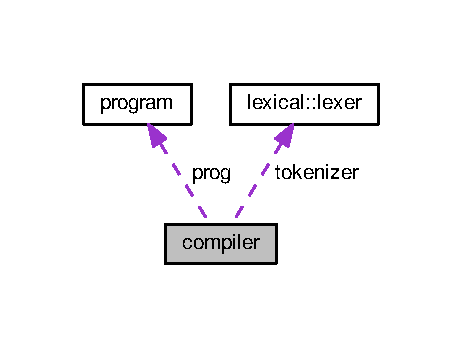
\includegraphics[width=222pt]{classcompiler__coll__graph}
\end{center}
\end{figure}
\subsection*{Public Member Functions}
\begin{DoxyCompactItemize}
\item 
\hyperlink{classcompiler_aac603e3e8c3851dfb420e6e007adbad0}{compiler} (\hyperlink{classlexical_1_1lexer}{lexical\+::lexer} \&\hyperlink{classcompiler_a888ac16dbb82fa8a9500633addcd22ba}{tokenizer}, vector$<$ \hyperlink{namespaceparser_a85b2df48287fddaca144a5f6c01b4761}{parser\+::ruleptr} $>$ \&\hyperlink{classcompiler_a1b712963929882f359df919ce73bbf4e}{rules}, vector$<$ \hyperlink{classqasm_1_1exec_1_1executable}{qasm\+::exec\+::executable} $\ast$($\ast$)(\hyperlink{structparser_1_1parsetree}{parser\+::parsetree} \&)$>$ \&\hyperlink{classcompiler_a76cbb22ce5238f2fd9b3946f541dba0c}{converters}, vector$<$ void($\ast$)(\hyperlink{classcompiler}{compiler} \&, \hyperlink{classqasm_1_1exec_1_1executable}{qasm\+::exec\+::executable} $\ast$)$>$ \&\hyperlink{classcompiler_aa9d1b362adff0ca48511cf824ca1fe4c}{events}, \hyperlink{classprogram}{program} \&\hyperlink{classcompiler_a801700690bf711169679cb6ca890168a}{prog})
\item 
bool \hyperlink{classcompiler_af3984a0a53279c28bee8aee4b0ef84ca}{try\+\_\+parse\+\_\+file} (std\+::string filename)
\end{DoxyCompactItemize}
\subsection*{Public Attributes}
\begin{DoxyCompactItemize}
\item 
\hyperlink{classlexical_1_1lexer}{lexical\+::lexer} \& \hyperlink{classcompiler_a888ac16dbb82fa8a9500633addcd22ba}{tokenizer}
\item 
vector$<$ \hyperlink{namespaceparser_a85b2df48287fddaca144a5f6c01b4761}{parser\+::ruleptr} $>$ \& \hyperlink{classcompiler_a1b712963929882f359df919ce73bbf4e}{rules}
\item 
vector$<$ \hyperlink{classqasm_1_1exec_1_1executable}{qasm\+::exec\+::executable} $\ast$($\ast$)(\hyperlink{structparser_1_1parsetree}{parser\+::parsetree} \&)$>$ \& \hyperlink{classcompiler_a76cbb22ce5238f2fd9b3946f541dba0c}{converters}
\item 
vector$<$ void($\ast$)(\hyperlink{classcompiler}{compiler} \&, \hyperlink{classqasm_1_1exec_1_1executable}{qasm\+::exec\+::executable} $\ast$)$>$ \& \hyperlink{classcompiler_aa9d1b362adff0ca48511cf824ca1fe4c}{events}
\item 
\hyperlink{classprogram}{program} \& \hyperlink{classcompiler_a801700690bf711169679cb6ca890168a}{prog}
\end{DoxyCompactItemize}


\subsection{Detailed Description}
Class wrapping up all compiler components 

\subsection{Constructor \& Destructor Documentation}
\index{compiler@{compiler}!compiler@{compiler}}
\index{compiler@{compiler}!compiler@{compiler}}
\subsubsection[{\texorpdfstring{compiler(lexical\+::lexer \&tokenizer, vector$<$ parser\+::ruleptr $>$ \&rules, vector$<$ qasm\+::exec\+::executable $\ast$($\ast$)(parser\+::parsetree \&)$>$ \&converters, vector$<$ void($\ast$)(compiler \&, qasm\+::exec\+::executable $\ast$)$>$ \&events, program \&prog)}{compiler(lexical::lexer &tokenizer, vector< parser::ruleptr > &rules, vector< qasm::exec::executable *(*)(parser::parsetree &)> &converters, vector< void(*)(compiler &, qasm::exec::executable *)> &events, program &prog)}}]{\setlength{\rightskip}{0pt plus 5cm}compiler\+::compiler (
\begin{DoxyParamCaption}
\item[{{\bf lexical\+::lexer} \&}]{tokenizer, }
\item[{vector$<$ {\bf parser\+::ruleptr} $>$ \&}]{rules, }
\item[{vector$<$ {\bf qasm\+::exec\+::executable} $\ast$($\ast$)({\bf parser\+::parsetree} \&)$>$ \&}]{converters, }
\item[{vector$<$ void($\ast$)({\bf compiler} \&, {\bf qasm\+::exec\+::executable} $\ast$)$>$ \&}]{events, }
\item[{{\bf program} \&}]{prog}
\end{DoxyParamCaption}
)\hspace{0.3cm}{\ttfamily [inline]}}\hypertarget{classcompiler_aac603e3e8c3851dfb420e6e007adbad0}{}\label{classcompiler_aac603e3e8c3851dfb420e6e007adbad0}


\subsection{Member Function Documentation}
\index{compiler@{compiler}!try\+\_\+parse\+\_\+file@{try\+\_\+parse\+\_\+file}}
\index{try\+\_\+parse\+\_\+file@{try\+\_\+parse\+\_\+file}!compiler@{compiler}}
\subsubsection[{\texorpdfstring{try\+\_\+parse\+\_\+file(std\+::string filename)}{try_parse_file(std::string filename)}}]{\setlength{\rightskip}{0pt plus 5cm}bool compiler\+::try\+\_\+parse\+\_\+file (
\begin{DoxyParamCaption}
\item[{std\+::string}]{filename}
\end{DoxyParamCaption}
)\hspace{0.3cm}{\ttfamily [inline]}}\hypertarget{classcompiler_af3984a0a53279c28bee8aee4b0ef84ca}{}\label{classcompiler_af3984a0a53279c28bee8aee4b0ef84ca}


\subsection{Member Data Documentation}
\index{compiler@{compiler}!converters@{converters}}
\index{converters@{converters}!compiler@{compiler}}
\subsubsection[{\texorpdfstring{converters}{converters}}]{\setlength{\rightskip}{0pt plus 5cm}vector$<${\bf qasm\+::exec\+::executable}$\ast$ ($\ast$)({\bf parser\+::parsetree}\&)$>$\& compiler\+::converters}\hypertarget{classcompiler_a76cbb22ce5238f2fd9b3946f541dba0c}{}\label{classcompiler_a76cbb22ce5238f2fd9b3946f541dba0c}
\index{compiler@{compiler}!events@{events}}
\index{events@{events}!compiler@{compiler}}
\subsubsection[{\texorpdfstring{events}{events}}]{\setlength{\rightskip}{0pt plus 5cm}vector$<$void($\ast$)({\bf compiler}\&, {\bf qasm\+::exec\+::executable}$\ast$)$>$\& compiler\+::events}\hypertarget{classcompiler_aa9d1b362adff0ca48511cf824ca1fe4c}{}\label{classcompiler_aa9d1b362adff0ca48511cf824ca1fe4c}
\index{compiler@{compiler}!prog@{prog}}
\index{prog@{prog}!compiler@{compiler}}
\subsubsection[{\texorpdfstring{prog}{prog}}]{\setlength{\rightskip}{0pt plus 5cm}{\bf program}\& compiler\+::prog}\hypertarget{classcompiler_a801700690bf711169679cb6ca890168a}{}\label{classcompiler_a801700690bf711169679cb6ca890168a}
\index{compiler@{compiler}!rules@{rules}}
\index{rules@{rules}!compiler@{compiler}}
\subsubsection[{\texorpdfstring{rules}{rules}}]{\setlength{\rightskip}{0pt plus 5cm}vector$<${\bf parser\+::ruleptr}$>$\& compiler\+::rules}\hypertarget{classcompiler_a1b712963929882f359df919ce73bbf4e}{}\label{classcompiler_a1b712963929882f359df919ce73bbf4e}
\index{compiler@{compiler}!tokenizer@{tokenizer}}
\index{tokenizer@{tokenizer}!compiler@{compiler}}
\subsubsection[{\texorpdfstring{tokenizer}{tokenizer}}]{\setlength{\rightskip}{0pt plus 5cm}{\bf lexical\+::lexer}\& compiler\+::tokenizer}\hypertarget{classcompiler_a888ac16dbb82fa8a9500633addcd22ba}{}\label{classcompiler_a888ac16dbb82fa8a9500633addcd22ba}


The documentation for this class was generated from the following file\+:\begin{DoxyCompactItemize}
\item 
src/runtime/\hyperlink{compiler_8hpp}{compiler.\+hpp}\end{DoxyCompactItemize}

\hypertarget{classqlib_1_1math_1_1complex}{}\section{qlib\+:\+:math\+:\+:complex Class Reference}
\label{classqlib_1_1math_1_1complex}\index{qlib\+::math\+::complex@{qlib\+::math\+::complex}}


{\ttfamily \#include $<$complex.\+hpp$>$}



Inheritance diagram for qlib\+:\+:math\+:\+:complex\+:\nopagebreak
\begin{figure}[H]
\begin{center}
\leavevmode
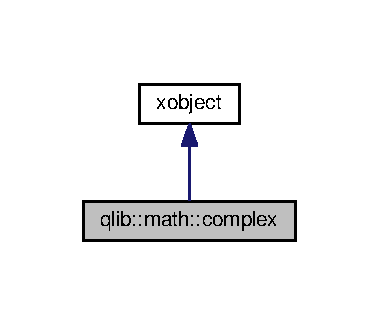
\includegraphics[width=182pt]{classqlib_1_1math_1_1complex__inherit__graph}
\end{center}
\end{figure}


Collaboration diagram for qlib\+:\+:math\+:\+:complex\+:\nopagebreak
\begin{figure}[H]
\begin{center}
\leavevmode
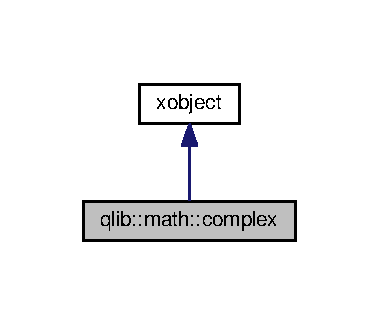
\includegraphics[width=182pt]{classqlib_1_1math_1_1complex__coll__graph}
\end{center}
\end{figure}
\subsection*{Public Member Functions}
\begin{DoxyCompactItemize}
\item 
\hyperlink{classqlib_1_1math_1_1complex_ab644fd7573e2bdbbfc02cf95b3fcdf62}{complex} ()
\item 
\hyperlink{classqlib_1_1math_1_1complex_a0eeea99f7c7d4a8e072f6c4836379ed0}{complex} (f32 real)
\item 
\hyperlink{classqlib_1_1math_1_1complex_a0dd3216eb1b24c906b394e67c59adda1}{complex} (f32 real, f32 img)
\item 
\hyperlink{classqlib_1_1math_1_1complex_ab1471e90345a25e6d112216f1a634290}{complex} (const \hyperlink{classqlib_1_1math_1_1complex}{complex} \&other)
\item 
f32 \hyperlink{classqlib_1_1math_1_1complex_ad1a8ab1ad95a47206e72d3a0d7be9511}{sqr\+Magnitude} ()
\item 
f32 \hyperlink{classqlib_1_1math_1_1complex_a8b365d2760802f1318e02c78c8938d2f}{magnitude} ()
\item 
\hyperlink{classqlib_1_1math_1_1complex}{complex} \hyperlink{classqlib_1_1math_1_1complex_a2cfd8546410a48d0568996e40beb85ce}{conjugate} ()
\item 
\hyperlink{classqlib_1_1math_1_1complex}{complex} \hyperlink{classqlib_1_1math_1_1complex_a088dcd1f0349632d0930177e95aa4729}{normal} ()
\item 
bool \hyperlink{classqlib_1_1math_1_1complex_a7a670edef0db4264e211e68aea71f0ec}{is\+Pure\+Real} ()
\item 
bool \hyperlink{classqlib_1_1math_1_1complex_a4465bc164fe2b490c917fc9321530ebb}{is\+Pure\+Imaginary} ()
\item 
bool \hyperlink{classqlib_1_1math_1_1complex_ae8f4008d499a05bbebecd48e0bf504d7}{is\+Zero} ()
\item 
f32 \hyperlink{classqlib_1_1math_1_1complex_a760122d26f377b008e129ff92b134a43}{arg} ()
\item 
std\+::string \hyperlink{classqlib_1_1math_1_1complex_afd24fadb21a07815675481b131398cff}{to\+String} ()
\end{DoxyCompactItemize}
\subsection*{Public Attributes}
\begin{DoxyCompactItemize}
\item 
f32 \hyperlink{classqlib_1_1math_1_1complex_aceb455ba091019bbd625fdaf529a0107}{r}
\item 
f32 \hyperlink{classqlib_1_1math_1_1complex_a4d599b5885fd37c300cdb79433356bb5}{i}
\end{DoxyCompactItemize}


\subsection{Detailed Description}
Object representation of a complex number in the form a + ib; 

\subsection{Constructor \& Destructor Documentation}
\index{qlib\+::math\+::complex@{qlib\+::math\+::complex}!complex@{complex}}
\index{complex@{complex}!qlib\+::math\+::complex@{qlib\+::math\+::complex}}
\subsubsection[{\texorpdfstring{complex()}{complex()}}]{\setlength{\rightskip}{0pt plus 5cm}qlib\+::math\+::complex\+::complex (
\begin{DoxyParamCaption}
{}
\end{DoxyParamCaption}
)\hspace{0.3cm}{\ttfamily [inline]}}\hypertarget{classqlib_1_1math_1_1complex_ab644fd7573e2bdbbfc02cf95b3fcdf62}{}\label{classqlib_1_1math_1_1complex_ab644fd7573e2bdbbfc02cf95b3fcdf62}
Create a complex number representing 0 + 0i \index{qlib\+::math\+::complex@{qlib\+::math\+::complex}!complex@{complex}}
\index{complex@{complex}!qlib\+::math\+::complex@{qlib\+::math\+::complex}}
\subsubsection[{\texorpdfstring{complex(f32 real)}{complex(f32 real)}}]{\setlength{\rightskip}{0pt plus 5cm}qlib\+::math\+::complex\+::complex (
\begin{DoxyParamCaption}
\item[{f32}]{real}
\end{DoxyParamCaption}
)\hspace{0.3cm}{\ttfamily [inline]}}\hypertarget{classqlib_1_1math_1_1complex_a0eeea99f7c7d4a8e072f6c4836379ed0}{}\label{classqlib_1_1math_1_1complex_a0eeea99f7c7d4a8e072f6c4836379ed0}
Create a complex number representing real + 0i \index{qlib\+::math\+::complex@{qlib\+::math\+::complex}!complex@{complex}}
\index{complex@{complex}!qlib\+::math\+::complex@{qlib\+::math\+::complex}}
\subsubsection[{\texorpdfstring{complex(f32 real, f32 img)}{complex(f32 real, f32 img)}}]{\setlength{\rightskip}{0pt plus 5cm}qlib\+::math\+::complex\+::complex (
\begin{DoxyParamCaption}
\item[{f32}]{real, }
\item[{f32}]{img}
\end{DoxyParamCaption}
)\hspace{0.3cm}{\ttfamily [inline]}}\hypertarget{classqlib_1_1math_1_1complex_a0dd3216eb1b24c906b394e67c59adda1}{}\label{classqlib_1_1math_1_1complex_a0dd3216eb1b24c906b394e67c59adda1}
Create a complex number representing real + img i \index{qlib\+::math\+::complex@{qlib\+::math\+::complex}!complex@{complex}}
\index{complex@{complex}!qlib\+::math\+::complex@{qlib\+::math\+::complex}}
\subsubsection[{\texorpdfstring{complex(const complex \&other)}{complex(const complex &other)}}]{\setlength{\rightskip}{0pt plus 5cm}qlib\+::math\+::complex\+::complex (
\begin{DoxyParamCaption}
\item[{const {\bf complex} \&}]{other}
\end{DoxyParamCaption}
)\hspace{0.3cm}{\ttfamily [inline]}}\hypertarget{classqlib_1_1math_1_1complex_ab1471e90345a25e6d112216f1a634290}{}\label{classqlib_1_1math_1_1complex_ab1471e90345a25e6d112216f1a634290}
Create a complex number from another 

\subsection{Member Function Documentation}
\index{qlib\+::math\+::complex@{qlib\+::math\+::complex}!arg@{arg}}
\index{arg@{arg}!qlib\+::math\+::complex@{qlib\+::math\+::complex}}
\subsubsection[{\texorpdfstring{arg()}{arg()}}]{\setlength{\rightskip}{0pt plus 5cm}f32 qlib\+::math\+::complex\+::arg (
\begin{DoxyParamCaption}
{}
\end{DoxyParamCaption}
)\hspace{0.3cm}{\ttfamily [inline]}}\hypertarget{classqlib_1_1math_1_1complex_a760122d26f377b008e129ff92b134a43}{}\label{classqlib_1_1math_1_1complex_a760122d26f377b008e129ff92b134a43}
Complex argument \index{qlib\+::math\+::complex@{qlib\+::math\+::complex}!conjugate@{conjugate}}
\index{conjugate@{conjugate}!qlib\+::math\+::complex@{qlib\+::math\+::complex}}
\subsubsection[{\texorpdfstring{conjugate()}{conjugate()}}]{\setlength{\rightskip}{0pt plus 5cm}{\bf complex} qlib\+::math\+::complex\+::conjugate (
\begin{DoxyParamCaption}
{}
\end{DoxyParamCaption}
)\hspace{0.3cm}{\ttfamily [inline]}}\hypertarget{classqlib_1_1math_1_1complex_a2cfd8546410a48d0568996e40beb85ce}{}\label{classqlib_1_1math_1_1complex_a2cfd8546410a48d0568996e40beb85ce}
Returns the complex conjugate of this number \index{qlib\+::math\+::complex@{qlib\+::math\+::complex}!is\+Pure\+Imaginary@{is\+Pure\+Imaginary}}
\index{is\+Pure\+Imaginary@{is\+Pure\+Imaginary}!qlib\+::math\+::complex@{qlib\+::math\+::complex}}
\subsubsection[{\texorpdfstring{is\+Pure\+Imaginary()}{isPureImaginary()}}]{\setlength{\rightskip}{0pt plus 5cm}bool qlib\+::math\+::complex\+::is\+Pure\+Imaginary (
\begin{DoxyParamCaption}
{}
\end{DoxyParamCaption}
)\hspace{0.3cm}{\ttfamily [inline]}}\hypertarget{classqlib_1_1math_1_1complex_a4465bc164fe2b490c917fc9321530ebb}{}\label{classqlib_1_1math_1_1complex_a4465bc164fe2b490c917fc9321530ebb}
Checks if this complex number can be represented as a purely imaginary number \index{qlib\+::math\+::complex@{qlib\+::math\+::complex}!is\+Pure\+Real@{is\+Pure\+Real}}
\index{is\+Pure\+Real@{is\+Pure\+Real}!qlib\+::math\+::complex@{qlib\+::math\+::complex}}
\subsubsection[{\texorpdfstring{is\+Pure\+Real()}{isPureReal()}}]{\setlength{\rightskip}{0pt plus 5cm}bool qlib\+::math\+::complex\+::is\+Pure\+Real (
\begin{DoxyParamCaption}
{}
\end{DoxyParamCaption}
)\hspace{0.3cm}{\ttfamily [inline]}}\hypertarget{classqlib_1_1math_1_1complex_a7a670edef0db4264e211e68aea71f0ec}{}\label{classqlib_1_1math_1_1complex_a7a670edef0db4264e211e68aea71f0ec}
Checks if this complex number can be represented as a purely real number \index{qlib\+::math\+::complex@{qlib\+::math\+::complex}!is\+Zero@{is\+Zero}}
\index{is\+Zero@{is\+Zero}!qlib\+::math\+::complex@{qlib\+::math\+::complex}}
\subsubsection[{\texorpdfstring{is\+Zero()}{isZero()}}]{\setlength{\rightskip}{0pt plus 5cm}bool qlib\+::math\+::complex\+::is\+Zero (
\begin{DoxyParamCaption}
{}
\end{DoxyParamCaption}
)\hspace{0.3cm}{\ttfamily [inline]}}\hypertarget{classqlib_1_1math_1_1complex_ae8f4008d499a05bbebecd48e0bf504d7}{}\label{classqlib_1_1math_1_1complex_ae8f4008d499a05bbebecd48e0bf504d7}
Checks if this complex number is zero \index{qlib\+::math\+::complex@{qlib\+::math\+::complex}!magnitude@{magnitude}}
\index{magnitude@{magnitude}!qlib\+::math\+::complex@{qlib\+::math\+::complex}}
\subsubsection[{\texorpdfstring{magnitude()}{magnitude()}}]{\setlength{\rightskip}{0pt plus 5cm}f32 qlib\+::math\+::complex\+::magnitude (
\begin{DoxyParamCaption}
{}
\end{DoxyParamCaption}
)\hspace{0.3cm}{\ttfamily [inline]}}\hypertarget{classqlib_1_1math_1_1complex_a8b365d2760802f1318e02c78c8938d2f}{}\label{classqlib_1_1math_1_1complex_a8b365d2760802f1318e02c78c8938d2f}
Magnitude of this complex number equals sqrt(abs(square magnitude)) \index{qlib\+::math\+::complex@{qlib\+::math\+::complex}!normal@{normal}}
\index{normal@{normal}!qlib\+::math\+::complex@{qlib\+::math\+::complex}}
\subsubsection[{\texorpdfstring{normal()}{normal()}}]{\setlength{\rightskip}{0pt plus 5cm}{\bf complex} qlib\+::math\+::complex\+::normal (
\begin{DoxyParamCaption}
{}
\end{DoxyParamCaption}
)\hspace{0.3cm}{\ttfamily [inline]}}\hypertarget{classqlib_1_1math_1_1complex_a088dcd1f0349632d0930177e95aa4729}{}\label{classqlib_1_1math_1_1complex_a088dcd1f0349632d0930177e95aa4729}
Returns a complex number of unit length but the same direction in the complex plane \index{qlib\+::math\+::complex@{qlib\+::math\+::complex}!sqr\+Magnitude@{sqr\+Magnitude}}
\index{sqr\+Magnitude@{sqr\+Magnitude}!qlib\+::math\+::complex@{qlib\+::math\+::complex}}
\subsubsection[{\texorpdfstring{sqr\+Magnitude()}{sqrMagnitude()}}]{\setlength{\rightskip}{0pt plus 5cm}f32 qlib\+::math\+::complex\+::sqr\+Magnitude (
\begin{DoxyParamCaption}
{}
\end{DoxyParamCaption}
)\hspace{0.3cm}{\ttfamily [inline]}}\hypertarget{classqlib_1_1math_1_1complex_ad1a8ab1ad95a47206e72d3a0d7be9511}{}\label{classqlib_1_1math_1_1complex_ad1a8ab1ad95a47206e72d3a0d7be9511}
Squared magnitude of this complex number equals this $\ast$ this-\/$>$\hyperlink{classqlib_1_1math_1_1complex_a2cfd8546410a48d0568996e40beb85ce}{conjugate()}. This is purely a real number. \index{qlib\+::math\+::complex@{qlib\+::math\+::complex}!to\+String@{to\+String}}
\index{to\+String@{to\+String}!qlib\+::math\+::complex@{qlib\+::math\+::complex}}
\subsubsection[{\texorpdfstring{to\+String()}{toString()}}]{\setlength{\rightskip}{0pt plus 5cm}std\+::string qlib\+::math\+::complex\+::to\+String (
\begin{DoxyParamCaption}
{}
\end{DoxyParamCaption}
)\hspace{0.3cm}{\ttfamily [inline]}, {\ttfamily [virtual]}}\hypertarget{classqlib_1_1math_1_1complex_afd24fadb21a07815675481b131398cff}{}\label{classqlib_1_1math_1_1complex_afd24fadb21a07815675481b131398cff}
String representation 

Reimplemented from \hyperlink{classxobject_ad76243a44c4e4959d3b16bb57d82600d}{xobject}.



\subsection{Member Data Documentation}
\index{qlib\+::math\+::complex@{qlib\+::math\+::complex}!i@{i}}
\index{i@{i}!qlib\+::math\+::complex@{qlib\+::math\+::complex}}
\subsubsection[{\texorpdfstring{i}{i}}]{\setlength{\rightskip}{0pt plus 5cm}f32 qlib\+::math\+::complex\+::i}\hypertarget{classqlib_1_1math_1_1complex_a4d599b5885fd37c300cdb79433356bb5}{}\label{classqlib_1_1math_1_1complex_a4d599b5885fd37c300cdb79433356bb5}
Imaginary component \index{qlib\+::math\+::complex@{qlib\+::math\+::complex}!r@{r}}
\index{r@{r}!qlib\+::math\+::complex@{qlib\+::math\+::complex}}
\subsubsection[{\texorpdfstring{r}{r}}]{\setlength{\rightskip}{0pt plus 5cm}f32 qlib\+::math\+::complex\+::r}\hypertarget{classqlib_1_1math_1_1complex_aceb455ba091019bbd625fdaf529a0107}{}\label{classqlib_1_1math_1_1complex_aceb455ba091019bbd625fdaf529a0107}
Real component 

The documentation for this class was generated from the following file\+:\begin{DoxyCompactItemize}
\item 
src/core/math/\hyperlink{complex_8hpp}{complex.\+hpp}\end{DoxyCompactItemize}

\hypertarget{classqlib_1_1quantum_1_1gates_1_1controlled2gate}{}\section{qlib\+:\+:quantum\+:\+:gates\+:\+:controlled2gate Class Reference}
\label{classqlib_1_1quantum_1_1gates_1_1controlled2gate}\index{qlib\+::quantum\+::gates\+::controlled2gate@{qlib\+::quantum\+::gates\+::controlled2gate}}


{\ttfamily \#include $<$controlled2gate.\+hpp$>$}



Inheritance diagram for qlib\+:\+:quantum\+:\+:gates\+:\+:controlled2gate\+:\nopagebreak
\begin{figure}[H]
\begin{center}
\leavevmode
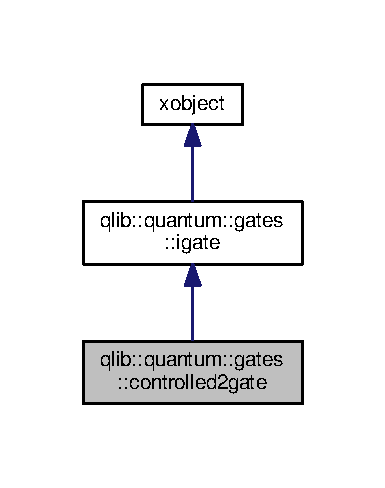
\includegraphics[width=185pt]{classqlib_1_1quantum_1_1gates_1_1controlled2gate__inherit__graph}
\end{center}
\end{figure}


Collaboration diagram for qlib\+:\+:quantum\+:\+:gates\+:\+:controlled2gate\+:\nopagebreak
\begin{figure}[H]
\begin{center}
\leavevmode
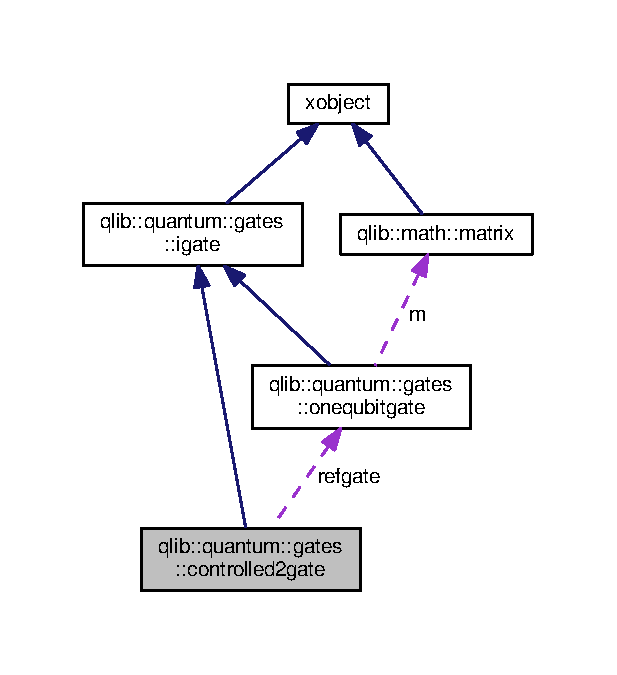
\includegraphics[width=296pt]{classqlib_1_1quantum_1_1gates_1_1controlled2gate__coll__graph}
\end{center}
\end{figure}
\subsection*{Public Member Functions}
\begin{DoxyCompactItemize}
\item 
\hyperlink{classqlib_1_1quantum_1_1gates_1_1controlled2gate_a83775bed048e4856d99c8d59d6a20db3}{controlled2gate} (std\+::string \hyperlink{classqlib_1_1quantum_1_1gates_1_1controlled2gate_a25121d9bc52a594a718b6d8037ea6cc0}{name}, \hyperlink{classqlib_1_1quantum_1_1gates_1_1onequbitgate}{onequbitgate} \&gate)
\item 
size\+\_\+t \hyperlink{classqlib_1_1quantum_1_1gates_1_1controlled2gate_a27a8793a3015aa9797f03fa0174113c2}{inputs} ()
\item 
std\+::string \hyperlink{classqlib_1_1quantum_1_1gates_1_1controlled2gate_a25121d9bc52a594a718b6d8037ea6cc0}{name} ()
\item 
void \hyperlink{classqlib_1_1quantum_1_1gates_1_1controlled2gate_a272635da6a7b8f65379f6ecb42df9389}{operate} (\hyperlink{classqlib_1_1math_1_1matrix}{matrix} \&in, \hyperlink{classqlib_1_1math_1_1matrix}{matrix} \&out, std\+::vector$<$ u64 $>$ input\+Qubits)
\item 
\hyperlink{classqlib_1_1math_1_1matrix}{qlib\+::math\+::matrix} \& \hyperlink{classqlib_1_1quantum_1_1gates_1_1controlled2gate_aeefab300e88034edbb5eacfa882ed218}{get\+Matrix} ()
\item 
std\+::string \hyperlink{classqlib_1_1quantum_1_1gates_1_1controlled2gate_a4fda814b0336d103f5cdb7ea98507bd1}{to\+String} ()
\end{DoxyCompactItemize}
\subsection*{Private Attributes}
\begin{DoxyCompactItemize}
\item 
std\+::string \hyperlink{classqlib_1_1quantum_1_1gates_1_1controlled2gate_a32ec87dafda9c4c80af4dc93758f6275}{sname}
\item 
\hyperlink{classqlib_1_1quantum_1_1gates_1_1onequbitgate}{onequbitgate} \& \hyperlink{classqlib_1_1quantum_1_1gates_1_1controlled2gate_abb21342d2206fbc4f7ab4e781997e471}{refgate}
\end{DoxyCompactItemize}


\subsection{Constructor \& Destructor Documentation}
\index{qlib\+::quantum\+::gates\+::controlled2gate@{qlib\+::quantum\+::gates\+::controlled2gate}!controlled2gate@{controlled2gate}}
\index{controlled2gate@{controlled2gate}!qlib\+::quantum\+::gates\+::controlled2gate@{qlib\+::quantum\+::gates\+::controlled2gate}}
\subsubsection[{\texorpdfstring{controlled2gate(std\+::string name, onequbitgate \&gate)}{controlled2gate(std::string name, onequbitgate &gate)}}]{\setlength{\rightskip}{0pt plus 5cm}qlib\+::quantum\+::gates\+::controlled2gate\+::controlled2gate (
\begin{DoxyParamCaption}
\item[{std\+::string}]{name, }
\item[{{\bf onequbitgate} \&}]{gate}
\end{DoxyParamCaption}
)\hspace{0.3cm}{\ttfamily [inline]}}\hypertarget{classqlib_1_1quantum_1_1gates_1_1controlled2gate_a83775bed048e4856d99c8d59d6a20db3}{}\label{classqlib_1_1quantum_1_1gates_1_1controlled2gate_a83775bed048e4856d99c8d59d6a20db3}
Create a new quanutm operator for the given number of states 

\subsection{Member Function Documentation}
\index{qlib\+::quantum\+::gates\+::controlled2gate@{qlib\+::quantum\+::gates\+::controlled2gate}!get\+Matrix@{get\+Matrix}}
\index{get\+Matrix@{get\+Matrix}!qlib\+::quantum\+::gates\+::controlled2gate@{qlib\+::quantum\+::gates\+::controlled2gate}}
\subsubsection[{\texorpdfstring{get\+Matrix()}{getMatrix()}}]{\setlength{\rightskip}{0pt plus 5cm}{\bf qlib\+::math\+::matrix}\& qlib\+::quantum\+::gates\+::controlled2gate\+::get\+Matrix (
\begin{DoxyParamCaption}
{}
\end{DoxyParamCaption}
)\hspace{0.3cm}{\ttfamily [inline]}}\hypertarget{classqlib_1_1quantum_1_1gates_1_1controlled2gate_aeefab300e88034edbb5eacfa882ed218}{}\label{classqlib_1_1quantum_1_1gates_1_1controlled2gate_aeefab300e88034edbb5eacfa882ed218}
Returns the matrix representation of this operator \index{qlib\+::quantum\+::gates\+::controlled2gate@{qlib\+::quantum\+::gates\+::controlled2gate}!inputs@{inputs}}
\index{inputs@{inputs}!qlib\+::quantum\+::gates\+::controlled2gate@{qlib\+::quantum\+::gates\+::controlled2gate}}
\subsubsection[{\texorpdfstring{inputs()}{inputs()}}]{\setlength{\rightskip}{0pt plus 5cm}size\+\_\+t qlib\+::quantum\+::gates\+::controlled2gate\+::inputs (
\begin{DoxyParamCaption}
{}
\end{DoxyParamCaption}
)\hspace{0.3cm}{\ttfamily [inline]}, {\ttfamily [virtual]}}\hypertarget{classqlib_1_1quantum_1_1gates_1_1controlled2gate_a27a8793a3015aa9797f03fa0174113c2}{}\label{classqlib_1_1quantum_1_1gates_1_1controlled2gate_a27a8793a3015aa9797f03fa0174113c2}
Number of input qubits this operator can be applied to 

Implements \hyperlink{classqlib_1_1quantum_1_1gates_1_1igate_ac8aa56b0095a94fdd437bc55d90aec9d}{qlib\+::quantum\+::gates\+::igate}.

\index{qlib\+::quantum\+::gates\+::controlled2gate@{qlib\+::quantum\+::gates\+::controlled2gate}!name@{name}}
\index{name@{name}!qlib\+::quantum\+::gates\+::controlled2gate@{qlib\+::quantum\+::gates\+::controlled2gate}}
\subsubsection[{\texorpdfstring{name()}{name()}}]{\setlength{\rightskip}{0pt plus 5cm}std\+::string qlib\+::quantum\+::gates\+::controlled2gate\+::name (
\begin{DoxyParamCaption}
{}
\end{DoxyParamCaption}
)\hspace{0.3cm}{\ttfamily [inline]}, {\ttfamily [virtual]}}\hypertarget{classqlib_1_1quantum_1_1gates_1_1controlled2gate_a25121d9bc52a594a718b6d8037ea6cc0}{}\label{classqlib_1_1quantum_1_1gates_1_1controlled2gate_a25121d9bc52a594a718b6d8037ea6cc0}
The name of this gate 

Implements \hyperlink{classqlib_1_1quantum_1_1gates_1_1igate_ae8f8dda69d7742c12c743829abb3662b}{qlib\+::quantum\+::gates\+::igate}.

\index{qlib\+::quantum\+::gates\+::controlled2gate@{qlib\+::quantum\+::gates\+::controlled2gate}!operate@{operate}}
\index{operate@{operate}!qlib\+::quantum\+::gates\+::controlled2gate@{qlib\+::quantum\+::gates\+::controlled2gate}}
\subsubsection[{\texorpdfstring{operate(matrix \&in, matrix \&out, std\+::vector$<$ u64 $>$ input\+Qubits)}{operate(matrix &in, matrix &out, std::vector< u64 > inputQubits)}}]{\setlength{\rightskip}{0pt plus 5cm}void qlib\+::quantum\+::gates\+::controlled2gate\+::operate (
\begin{DoxyParamCaption}
\item[{{\bf matrix} \&}]{in, }
\item[{{\bf matrix} \&}]{out, }
\item[{std\+::vector$<$ u64 $>$}]{input\+Qubits}
\end{DoxyParamCaption}
)\hspace{0.3cm}{\ttfamily [inline]}, {\ttfamily [virtual]}}\hypertarget{classqlib_1_1quantum_1_1gates_1_1controlled2gate_a272635da6a7b8f65379f6ecb42df9389}{}\label{classqlib_1_1quantum_1_1gates_1_1controlled2gate_a272635da6a7b8f65379f6ecb42df9389}
Operate on a given column vector state superposition 

Implements \hyperlink{classqlib_1_1quantum_1_1gates_1_1igate_a66038ee65fec12c627789505e11f1e23}{qlib\+::quantum\+::gates\+::igate}.

\index{qlib\+::quantum\+::gates\+::controlled2gate@{qlib\+::quantum\+::gates\+::controlled2gate}!to\+String@{to\+String}}
\index{to\+String@{to\+String}!qlib\+::quantum\+::gates\+::controlled2gate@{qlib\+::quantum\+::gates\+::controlled2gate}}
\subsubsection[{\texorpdfstring{to\+String()}{toString()}}]{\setlength{\rightskip}{0pt plus 5cm}std\+::string qlib\+::quantum\+::gates\+::controlled2gate\+::to\+String (
\begin{DoxyParamCaption}
{}
\end{DoxyParamCaption}
)\hspace{0.3cm}{\ttfamily [inline]}, {\ttfamily [virtual]}}\hypertarget{classqlib_1_1quantum_1_1gates_1_1controlled2gate_a4fda814b0336d103f5cdb7ea98507bd1}{}\label{classqlib_1_1quantum_1_1gates_1_1controlled2gate_a4fda814b0336d103f5cdb7ea98507bd1}
Pretty print 

Reimplemented from \hyperlink{classxobject_ad76243a44c4e4959d3b16bb57d82600d}{xobject}.



\subsection{Member Data Documentation}
\index{qlib\+::quantum\+::gates\+::controlled2gate@{qlib\+::quantum\+::gates\+::controlled2gate}!refgate@{refgate}}
\index{refgate@{refgate}!qlib\+::quantum\+::gates\+::controlled2gate@{qlib\+::quantum\+::gates\+::controlled2gate}}
\subsubsection[{\texorpdfstring{refgate}{refgate}}]{\setlength{\rightskip}{0pt plus 5cm}{\bf onequbitgate}\& qlib\+::quantum\+::gates\+::controlled2gate\+::refgate\hspace{0.3cm}{\ttfamily [private]}}\hypertarget{classqlib_1_1quantum_1_1gates_1_1controlled2gate_abb21342d2206fbc4f7ab4e781997e471}{}\label{classqlib_1_1quantum_1_1gates_1_1controlled2gate_abb21342d2206fbc4f7ab4e781997e471}
\index{qlib\+::quantum\+::gates\+::controlled2gate@{qlib\+::quantum\+::gates\+::controlled2gate}!sname@{sname}}
\index{sname@{sname}!qlib\+::quantum\+::gates\+::controlled2gate@{qlib\+::quantum\+::gates\+::controlled2gate}}
\subsubsection[{\texorpdfstring{sname}{sname}}]{\setlength{\rightskip}{0pt plus 5cm}std\+::string qlib\+::quantum\+::gates\+::controlled2gate\+::sname\hspace{0.3cm}{\ttfamily [private]}}\hypertarget{classqlib_1_1quantum_1_1gates_1_1controlled2gate_a32ec87dafda9c4c80af4dc93758f6275}{}\label{classqlib_1_1quantum_1_1gates_1_1controlled2gate_a32ec87dafda9c4c80af4dc93758f6275}


The documentation for this class was generated from the following file\+:\begin{DoxyCompactItemize}
\item 
src/core/quantum/gates/\hyperlink{controlled2gate_8hpp}{controlled2gate.\+hpp}\end{DoxyCompactItemize}

\hypertarget{classqlib_1_1quantum_1_1gates_1_1controlledgate}{}\section{qlib\+:\+:quantum\+:\+:gates\+:\+:controlledgate Class Reference}
\label{classqlib_1_1quantum_1_1gates_1_1controlledgate}\index{qlib\+::quantum\+::gates\+::controlledgate@{qlib\+::quantum\+::gates\+::controlledgate}}


{\ttfamily \#include $<$controlledgate.\+hpp$>$}



Inheritance diagram for qlib\+:\+:quantum\+:\+:gates\+:\+:controlledgate\+:\nopagebreak
\begin{figure}[H]
\begin{center}
\leavevmode
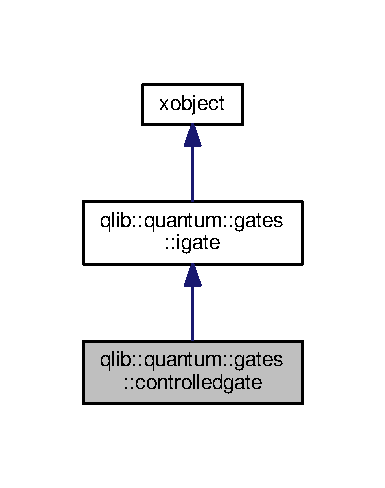
\includegraphics[width=185pt]{classqlib_1_1quantum_1_1gates_1_1controlledgate__inherit__graph}
\end{center}
\end{figure}


Collaboration diagram for qlib\+:\+:quantum\+:\+:gates\+:\+:controlledgate\+:\nopagebreak
\begin{figure}[H]
\begin{center}
\leavevmode
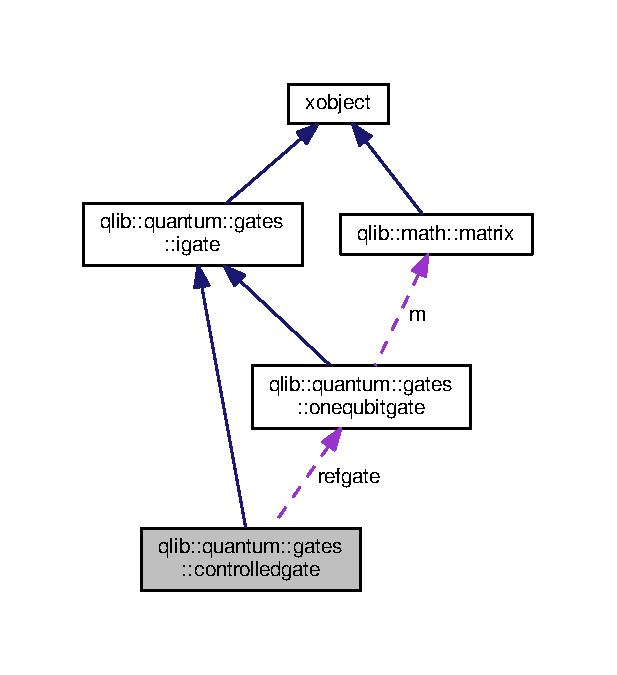
\includegraphics[width=296pt]{classqlib_1_1quantum_1_1gates_1_1controlledgate__coll__graph}
\end{center}
\end{figure}
\subsection*{Public Member Functions}
\begin{DoxyCompactItemize}
\item 
\hyperlink{classqlib_1_1quantum_1_1gates_1_1controlledgate_abe6d1d959a5a781739fe962551d013e7}{controlledgate} (std\+::string \hyperlink{classqlib_1_1quantum_1_1gates_1_1controlledgate_a7fb8875c83106b35d733cc96b312b957}{name}, \hyperlink{classqlib_1_1quantum_1_1gates_1_1onequbitgate}{onequbitgate} \&gate)
\item 
size\+\_\+t \hyperlink{classqlib_1_1quantum_1_1gates_1_1controlledgate_adb544cb10cd5f8836e331102f7c7e9d6}{inputs} ()
\item 
std\+::string \hyperlink{classqlib_1_1quantum_1_1gates_1_1controlledgate_a7fb8875c83106b35d733cc96b312b957}{name} ()
\item 
void \hyperlink{classqlib_1_1quantum_1_1gates_1_1controlledgate_aec6e423cc6ae442c5c3c5dc04581959e}{operate} (\hyperlink{classqlib_1_1math_1_1matrix}{matrix} \&in, \hyperlink{classqlib_1_1math_1_1matrix}{matrix} \&out, std\+::vector$<$ u64 $>$ input\+Qubits)
\item 
\hyperlink{classqlib_1_1math_1_1matrix}{qlib\+::math\+::matrix} \& \hyperlink{classqlib_1_1quantum_1_1gates_1_1controlledgate_a7d9d8771acebaa39b35176c04f114cb1}{get\+Matrix} ()
\item 
std\+::string \hyperlink{classqlib_1_1quantum_1_1gates_1_1controlledgate_a87b4d6e66acffc4e14eb3e39a19c4bee}{to\+String} ()
\end{DoxyCompactItemize}
\subsection*{Private Attributes}
\begin{DoxyCompactItemize}
\item 
std\+::string \hyperlink{classqlib_1_1quantum_1_1gates_1_1controlledgate_a638c7bead4c936bc0c8672a1fee4b50f}{sname}
\item 
\hyperlink{classqlib_1_1quantum_1_1gates_1_1onequbitgate}{onequbitgate} \& \hyperlink{classqlib_1_1quantum_1_1gates_1_1controlledgate_a8712f70ae76ec442aebad49109ddea97}{refgate}
\end{DoxyCompactItemize}


\subsection{Constructor \& Destructor Documentation}
\index{qlib\+::quantum\+::gates\+::controlledgate@{qlib\+::quantum\+::gates\+::controlledgate}!controlledgate@{controlledgate}}
\index{controlledgate@{controlledgate}!qlib\+::quantum\+::gates\+::controlledgate@{qlib\+::quantum\+::gates\+::controlledgate}}
\subsubsection[{\texorpdfstring{controlledgate(std\+::string name, onequbitgate \&gate)}{controlledgate(std::string name, onequbitgate &gate)}}]{\setlength{\rightskip}{0pt plus 5cm}qlib\+::quantum\+::gates\+::controlledgate\+::controlledgate (
\begin{DoxyParamCaption}
\item[{std\+::string}]{name, }
\item[{{\bf onequbitgate} \&}]{gate}
\end{DoxyParamCaption}
)\hspace{0.3cm}{\ttfamily [inline]}}\hypertarget{classqlib_1_1quantum_1_1gates_1_1controlledgate_abe6d1d959a5a781739fe962551d013e7}{}\label{classqlib_1_1quantum_1_1gates_1_1controlledgate_abe6d1d959a5a781739fe962551d013e7}
Create a new quanutm operator for the given number of states 

\subsection{Member Function Documentation}
\index{qlib\+::quantum\+::gates\+::controlledgate@{qlib\+::quantum\+::gates\+::controlledgate}!get\+Matrix@{get\+Matrix}}
\index{get\+Matrix@{get\+Matrix}!qlib\+::quantum\+::gates\+::controlledgate@{qlib\+::quantum\+::gates\+::controlledgate}}
\subsubsection[{\texorpdfstring{get\+Matrix()}{getMatrix()}}]{\setlength{\rightskip}{0pt plus 5cm}{\bf qlib\+::math\+::matrix}\& qlib\+::quantum\+::gates\+::controlledgate\+::get\+Matrix (
\begin{DoxyParamCaption}
{}
\end{DoxyParamCaption}
)\hspace{0.3cm}{\ttfamily [inline]}}\hypertarget{classqlib_1_1quantum_1_1gates_1_1controlledgate_a7d9d8771acebaa39b35176c04f114cb1}{}\label{classqlib_1_1quantum_1_1gates_1_1controlledgate_a7d9d8771acebaa39b35176c04f114cb1}
Returns the matrix representation of this operator \index{qlib\+::quantum\+::gates\+::controlledgate@{qlib\+::quantum\+::gates\+::controlledgate}!inputs@{inputs}}
\index{inputs@{inputs}!qlib\+::quantum\+::gates\+::controlledgate@{qlib\+::quantum\+::gates\+::controlledgate}}
\subsubsection[{\texorpdfstring{inputs()}{inputs()}}]{\setlength{\rightskip}{0pt plus 5cm}size\+\_\+t qlib\+::quantum\+::gates\+::controlledgate\+::inputs (
\begin{DoxyParamCaption}
{}
\end{DoxyParamCaption}
)\hspace{0.3cm}{\ttfamily [inline]}, {\ttfamily [virtual]}}\hypertarget{classqlib_1_1quantum_1_1gates_1_1controlledgate_adb544cb10cd5f8836e331102f7c7e9d6}{}\label{classqlib_1_1quantum_1_1gates_1_1controlledgate_adb544cb10cd5f8836e331102f7c7e9d6}
Number of input qubits this operator can be applied to 

Implements \hyperlink{classqlib_1_1quantum_1_1gates_1_1igate_ac8aa56b0095a94fdd437bc55d90aec9d}{qlib\+::quantum\+::gates\+::igate}.

\index{qlib\+::quantum\+::gates\+::controlledgate@{qlib\+::quantum\+::gates\+::controlledgate}!name@{name}}
\index{name@{name}!qlib\+::quantum\+::gates\+::controlledgate@{qlib\+::quantum\+::gates\+::controlledgate}}
\subsubsection[{\texorpdfstring{name()}{name()}}]{\setlength{\rightskip}{0pt plus 5cm}std\+::string qlib\+::quantum\+::gates\+::controlledgate\+::name (
\begin{DoxyParamCaption}
{}
\end{DoxyParamCaption}
)\hspace{0.3cm}{\ttfamily [inline]}, {\ttfamily [virtual]}}\hypertarget{classqlib_1_1quantum_1_1gates_1_1controlledgate_a7fb8875c83106b35d733cc96b312b957}{}\label{classqlib_1_1quantum_1_1gates_1_1controlledgate_a7fb8875c83106b35d733cc96b312b957}
The name of this gate 

Implements \hyperlink{classqlib_1_1quantum_1_1gates_1_1igate_ae8f8dda69d7742c12c743829abb3662b}{qlib\+::quantum\+::gates\+::igate}.

\index{qlib\+::quantum\+::gates\+::controlledgate@{qlib\+::quantum\+::gates\+::controlledgate}!operate@{operate}}
\index{operate@{operate}!qlib\+::quantum\+::gates\+::controlledgate@{qlib\+::quantum\+::gates\+::controlledgate}}
\subsubsection[{\texorpdfstring{operate(matrix \&in, matrix \&out, std\+::vector$<$ u64 $>$ input\+Qubits)}{operate(matrix &in, matrix &out, std::vector< u64 > inputQubits)}}]{\setlength{\rightskip}{0pt plus 5cm}void qlib\+::quantum\+::gates\+::controlledgate\+::operate (
\begin{DoxyParamCaption}
\item[{{\bf matrix} \&}]{in, }
\item[{{\bf matrix} \&}]{out, }
\item[{std\+::vector$<$ u64 $>$}]{input\+Qubits}
\end{DoxyParamCaption}
)\hspace{0.3cm}{\ttfamily [inline]}, {\ttfamily [virtual]}}\hypertarget{classqlib_1_1quantum_1_1gates_1_1controlledgate_aec6e423cc6ae442c5c3c5dc04581959e}{}\label{classqlib_1_1quantum_1_1gates_1_1controlledgate_aec6e423cc6ae442c5c3c5dc04581959e}
Operate on a given column vector state superposition 

Implements \hyperlink{classqlib_1_1quantum_1_1gates_1_1igate_a66038ee65fec12c627789505e11f1e23}{qlib\+::quantum\+::gates\+::igate}.

\index{qlib\+::quantum\+::gates\+::controlledgate@{qlib\+::quantum\+::gates\+::controlledgate}!to\+String@{to\+String}}
\index{to\+String@{to\+String}!qlib\+::quantum\+::gates\+::controlledgate@{qlib\+::quantum\+::gates\+::controlledgate}}
\subsubsection[{\texorpdfstring{to\+String()}{toString()}}]{\setlength{\rightskip}{0pt plus 5cm}std\+::string qlib\+::quantum\+::gates\+::controlledgate\+::to\+String (
\begin{DoxyParamCaption}
{}
\end{DoxyParamCaption}
)\hspace{0.3cm}{\ttfamily [inline]}, {\ttfamily [virtual]}}\hypertarget{classqlib_1_1quantum_1_1gates_1_1controlledgate_a87b4d6e66acffc4e14eb3e39a19c4bee}{}\label{classqlib_1_1quantum_1_1gates_1_1controlledgate_a87b4d6e66acffc4e14eb3e39a19c4bee}
Pretty print 

Reimplemented from \hyperlink{classxobject_ad76243a44c4e4959d3b16bb57d82600d}{xobject}.



\subsection{Member Data Documentation}
\index{qlib\+::quantum\+::gates\+::controlledgate@{qlib\+::quantum\+::gates\+::controlledgate}!refgate@{refgate}}
\index{refgate@{refgate}!qlib\+::quantum\+::gates\+::controlledgate@{qlib\+::quantum\+::gates\+::controlledgate}}
\subsubsection[{\texorpdfstring{refgate}{refgate}}]{\setlength{\rightskip}{0pt plus 5cm}{\bf onequbitgate}\& qlib\+::quantum\+::gates\+::controlledgate\+::refgate\hspace{0.3cm}{\ttfamily [private]}}\hypertarget{classqlib_1_1quantum_1_1gates_1_1controlledgate_a8712f70ae76ec442aebad49109ddea97}{}\label{classqlib_1_1quantum_1_1gates_1_1controlledgate_a8712f70ae76ec442aebad49109ddea97}
\index{qlib\+::quantum\+::gates\+::controlledgate@{qlib\+::quantum\+::gates\+::controlledgate}!sname@{sname}}
\index{sname@{sname}!qlib\+::quantum\+::gates\+::controlledgate@{qlib\+::quantum\+::gates\+::controlledgate}}
\subsubsection[{\texorpdfstring{sname}{sname}}]{\setlength{\rightskip}{0pt plus 5cm}std\+::string qlib\+::quantum\+::gates\+::controlledgate\+::sname\hspace{0.3cm}{\ttfamily [private]}}\hypertarget{classqlib_1_1quantum_1_1gates_1_1controlledgate_a638c7bead4c936bc0c8672a1fee4b50f}{}\label{classqlib_1_1quantum_1_1gates_1_1controlledgate_a638c7bead4c936bc0c8672a1fee4b50f}


The documentation for this class was generated from the following file\+:\begin{DoxyCompactItemize}
\item 
src/core/quantum/gates/\hyperlink{controlledgate_8hpp}{controlledgate.\+hpp}\end{DoxyCompactItemize}

\hypertarget{classqasm_1_1exec_1_1declaration}{}\section{qasm\+:\+:exec\+:\+:declaration Class Reference}
\label{classqasm_1_1exec_1_1declaration}\index{qasm\+::exec\+::declaration@{qasm\+::exec\+::declaration}}


{\ttfamily \#include $<$runtime.\+hpp$>$}



Inheritance diagram for qasm\+:\+:exec\+:\+:declaration\+:\nopagebreak
\begin{figure}[H]
\begin{center}
\leavevmode
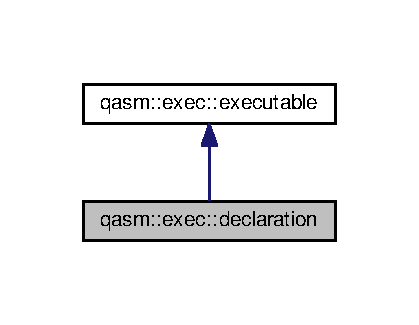
\includegraphics[width=201pt]{classqasm_1_1exec_1_1declaration__inherit__graph}
\end{center}
\end{figure}


Collaboration diagram for qasm\+:\+:exec\+:\+:declaration\+:\nopagebreak
\begin{figure}[H]
\begin{center}
\leavevmode
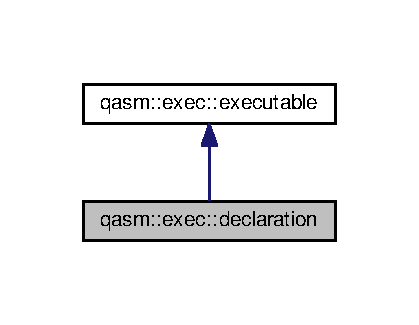
\includegraphics[width=201pt]{classqasm_1_1exec_1_1declaration__coll__graph}
\end{center}
\end{figure}
\subsection*{Public Member Functions}
\begin{DoxyCompactItemize}
\item 
\hyperlink{classqasm_1_1exec_1_1declaration_ae8f3a47af0a26055fb6fc90303defbeb}{declaration} (string t, string n, u64 s)
\item 
virtual void \hyperlink{classqasm_1_1exec_1_1declaration_a4f1396fca212fb0ce984d2cea90df0a8}{invoke\+\_\+rootprogram} (\hyperlink{classqasm_1_1runtime_1_1environment}{runtime\+::environment} \&env)
\end{DoxyCompactItemize}
\subsection*{Public Attributes}
\begin{DoxyCompactItemize}
\item 
std\+::string \hyperlink{classqasm_1_1exec_1_1declaration_a165d72745d002f80716cbd37f27687fe}{type}
\item 
std\+::string \hyperlink{classqasm_1_1exec_1_1declaration_a72faf3aa92a6a3d100ff0f7ddf0aab65}{name}
\item 
u64 \hyperlink{classqasm_1_1exec_1_1declaration_a53d08c265c26517db99871b3dd54cf89}{size}
\end{DoxyCompactItemize}


\subsection{Detailed Description}
Instruction to decare a variable 

\subsection{Constructor \& Destructor Documentation}
\index{qasm\+::exec\+::declaration@{qasm\+::exec\+::declaration}!declaration@{declaration}}
\index{declaration@{declaration}!qasm\+::exec\+::declaration@{qasm\+::exec\+::declaration}}
\subsubsection[{\texorpdfstring{declaration(string t, string n, u64 s)}{declaration(string t, string n, u64 s)}}]{\setlength{\rightskip}{0pt plus 5cm}qasm\+::exec\+::declaration\+::declaration (
\begin{DoxyParamCaption}
\item[{string}]{t, }
\item[{string}]{n, }
\item[{u64}]{s}
\end{DoxyParamCaption}
)\hspace{0.3cm}{\ttfamily [inline]}}\hypertarget{classqasm_1_1exec_1_1declaration_ae8f3a47af0a26055fb6fc90303defbeb}{}\label{classqasm_1_1exec_1_1declaration_ae8f3a47af0a26055fb6fc90303defbeb}


\subsection{Member Function Documentation}
\index{qasm\+::exec\+::declaration@{qasm\+::exec\+::declaration}!invoke\+\_\+rootprogram@{invoke\+\_\+rootprogram}}
\index{invoke\+\_\+rootprogram@{invoke\+\_\+rootprogram}!qasm\+::exec\+::declaration@{qasm\+::exec\+::declaration}}
\subsubsection[{\texorpdfstring{invoke\+\_\+rootprogram(runtime\+::environment \&env)}{invoke_rootprogram(runtime::environment &env)}}]{\setlength{\rightskip}{0pt plus 5cm}virtual void qasm\+::exec\+::declaration\+::invoke\+\_\+rootprogram (
\begin{DoxyParamCaption}
\item[{{\bf runtime\+::environment} \&}]{env}
\end{DoxyParamCaption}
)\hspace{0.3cm}{\ttfamily [inline]}, {\ttfamily [virtual]}}\hypertarget{classqasm_1_1exec_1_1declaration_a4f1396fca212fb0ce984d2cea90df0a8}{}\label{classqasm_1_1exec_1_1declaration_a4f1396fca212fb0ce984d2cea90df0a8}
Run instruction\textquotesingle{}s primary operation 

Reimplemented from \hyperlink{classqasm_1_1exec_1_1executable_ad07f864a889edb0777ebbb1bc1628121}{qasm\+::exec\+::executable}.



\subsection{Member Data Documentation}
\index{qasm\+::exec\+::declaration@{qasm\+::exec\+::declaration}!name@{name}}
\index{name@{name}!qasm\+::exec\+::declaration@{qasm\+::exec\+::declaration}}
\subsubsection[{\texorpdfstring{name}{name}}]{\setlength{\rightskip}{0pt plus 5cm}std\+::string qasm\+::exec\+::declaration\+::name}\hypertarget{classqasm_1_1exec_1_1declaration_a72faf3aa92a6a3d100ff0f7ddf0aab65}{}\label{classqasm_1_1exec_1_1declaration_a72faf3aa92a6a3d100ff0f7ddf0aab65}
Name of variable to declare \index{qasm\+::exec\+::declaration@{qasm\+::exec\+::declaration}!size@{size}}
\index{size@{size}!qasm\+::exec\+::declaration@{qasm\+::exec\+::declaration}}
\subsubsection[{\texorpdfstring{size}{size}}]{\setlength{\rightskip}{0pt plus 5cm}u64 qasm\+::exec\+::declaration\+::size}\hypertarget{classqasm_1_1exec_1_1declaration_a53d08c265c26517db99871b3dd54cf89}{}\label{classqasm_1_1exec_1_1declaration_a53d08c265c26517db99871b3dd54cf89}
Size of variable \index{qasm\+::exec\+::declaration@{qasm\+::exec\+::declaration}!type@{type}}
\index{type@{type}!qasm\+::exec\+::declaration@{qasm\+::exec\+::declaration}}
\subsubsection[{\texorpdfstring{type}{type}}]{\setlength{\rightskip}{0pt plus 5cm}std\+::string qasm\+::exec\+::declaration\+::type}\hypertarget{classqasm_1_1exec_1_1declaration_a165d72745d002f80716cbd37f27687fe}{}\label{classqasm_1_1exec_1_1declaration_a165d72745d002f80716cbd37f27687fe}
Type of variable to declare 

The documentation for this class was generated from the following file\+:\begin{DoxyCompactItemize}
\item 
src/runtime/\hyperlink{runtime_8hpp}{runtime.\+hpp}\end{DoxyCompactItemize}

\hypertarget{classqlib_1_1quantum_1_1ensemble}{}\section{qlib\+:\+:quantum\+:\+:ensemble Class Reference}
\label{classqlib_1_1quantum_1_1ensemble}\index{qlib\+::quantum\+::ensemble@{qlib\+::quantum\+::ensemble}}


{\ttfamily \#include $<$ensemble.\+hpp$>$}



Inheritance diagram for qlib\+:\+:quantum\+:\+:ensemble\+:\nopagebreak
\begin{figure}[H]
\begin{center}
\leavevmode
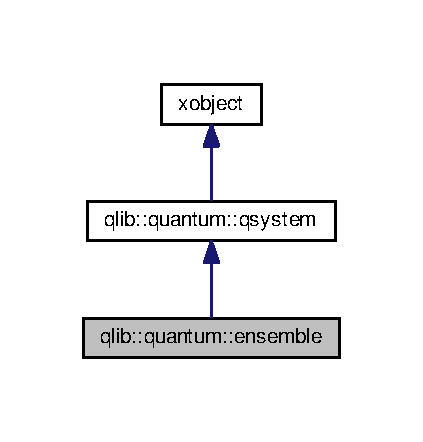
\includegraphics[width=203pt]{classqlib_1_1quantum_1_1ensemble__inherit__graph}
\end{center}
\end{figure}


Collaboration diagram for qlib\+:\+:quantum\+:\+:ensemble\+:\nopagebreak
\begin{figure}[H]
\begin{center}
\leavevmode
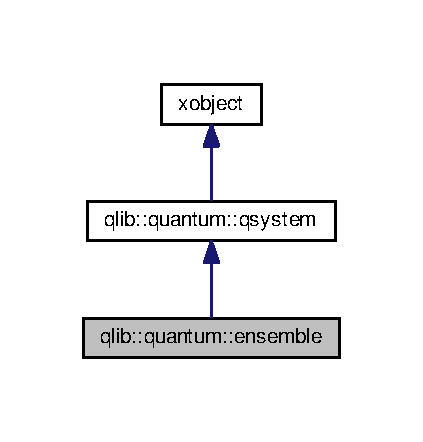
\includegraphics[width=203pt]{classqlib_1_1quantum_1_1ensemble__coll__graph}
\end{center}
\end{figure}
\subsection*{Public Member Functions}
\begin{DoxyCompactItemize}
\item 
\hyperlink{classqlib_1_1quantum_1_1ensemble_a5e088d9ac7394f150f5a2affe0790f2a}{ensemble} (std\+::vector$<$ \hyperlink{classqlib_1_1quantum_1_1qsystem}{qsystem} $\ast$ $>$ eset)
\item 
\hyperlink{classqlib_1_1quantum_1_1ensemble_aae0c56d2d64d4be27b5ab976d60c2747}{$\sim$ensemble} ()
\item 
size\+\_\+t \hyperlink{classqlib_1_1quantum_1_1ensemble_a4b811e4778f5c845504ed8eec058dfe4}{size} ()
\item 
void \hyperlink{classqlib_1_1quantum_1_1ensemble_a9226b1108f8d45d052316f7c366f1d5a}{apply} (\hyperlink{classqlib_1_1quantum_1_1gates_1_1igate}{qlib\+::quantum\+::gates\+::igate} \&op, std\+::vector$<$ u64 $>$ input\+Bits)
\item 
i8 \hyperlink{classqlib_1_1quantum_1_1ensemble_ae5e3ebd119e1df6dbb966b7bb6222e5a}{measure} (i64 \hyperlink{classqlib_1_1quantum_1_1qubit}{qubit})
\item 
virtual void \hyperlink{classqlib_1_1quantum_1_1ensemble_ac170f82a86704e08e8f2bebc721cf03b}{zero} (i64 \hyperlink{classqlib_1_1quantum_1_1qubit}{qubit})
\end{DoxyCompactItemize}
\subsection*{Private Attributes}
\begin{DoxyCompactItemize}
\item 
std\+::vector$<$ \hyperlink{classqlib_1_1quantum_1_1qsystem}{qsystem} $\ast$ $>$ \hyperlink{classqlib_1_1quantum_1_1ensemble_ab77e11f30898f29060ff97236ec26319}{set}
\end{DoxyCompactItemize}


\subsection{Detailed Description}
Represents a collection of multiple identical quantum systems 

\subsection{Constructor \& Destructor Documentation}
\index{qlib\+::quantum\+::ensemble@{qlib\+::quantum\+::ensemble}!ensemble@{ensemble}}
\index{ensemble@{ensemble}!qlib\+::quantum\+::ensemble@{qlib\+::quantum\+::ensemble}}
\subsubsection[{\texorpdfstring{ensemble(std\+::vector$<$ qsystem $\ast$ $>$ eset)}{ensemble(std::vector< qsystem * > eset)}}]{\setlength{\rightskip}{0pt plus 5cm}qlib\+::quantum\+::ensemble\+::ensemble (
\begin{DoxyParamCaption}
\item[{std\+::vector$<$ {\bf qsystem} $\ast$ $>$}]{eset}
\end{DoxyParamCaption}
)\hspace{0.3cm}{\ttfamily [inline]}}\hypertarget{classqlib_1_1quantum_1_1ensemble_a5e088d9ac7394f150f5a2affe0790f2a}{}\label{classqlib_1_1quantum_1_1ensemble_a5e088d9ac7394f150f5a2affe0790f2a}
Create an ensemble from a given list of systems \index{qlib\+::quantum\+::ensemble@{qlib\+::quantum\+::ensemble}!````~ensemble@{$\sim$ensemble}}
\index{````~ensemble@{$\sim$ensemble}!qlib\+::quantum\+::ensemble@{qlib\+::quantum\+::ensemble}}
\subsubsection[{\texorpdfstring{$\sim$ensemble()}{~ensemble()}}]{\setlength{\rightskip}{0pt plus 5cm}qlib\+::quantum\+::ensemble\+::$\sim$ensemble (
\begin{DoxyParamCaption}
{}
\end{DoxyParamCaption}
)\hspace{0.3cm}{\ttfamily [inline]}}\hypertarget{classqlib_1_1quantum_1_1ensemble_aae0c56d2d64d4be27b5ab976d60c2747}{}\label{classqlib_1_1quantum_1_1ensemble_aae0c56d2d64d4be27b5ab976d60c2747}
Delete the ensemble and cleanup pointers 

\subsection{Member Function Documentation}
\index{qlib\+::quantum\+::ensemble@{qlib\+::quantum\+::ensemble}!apply@{apply}}
\index{apply@{apply}!qlib\+::quantum\+::ensemble@{qlib\+::quantum\+::ensemble}}
\subsubsection[{\texorpdfstring{apply(qlib\+::quantum\+::gates\+::igate \&op, std\+::vector$<$ u64 $>$ input\+Bits)}{apply(qlib::quantum::gates::igate &op, std::vector< u64 > inputBits)}}]{\setlength{\rightskip}{0pt plus 5cm}void qlib\+::quantum\+::ensemble\+::apply (
\begin{DoxyParamCaption}
\item[{{\bf qlib\+::quantum\+::gates\+::igate} \&}]{op, }
\item[{std\+::vector$<$ u64 $>$}]{input\+Bits}
\end{DoxyParamCaption}
)\hspace{0.3cm}{\ttfamily [inline]}, {\ttfamily [virtual]}}\hypertarget{classqlib_1_1quantum_1_1ensemble_a9226b1108f8d45d052316f7c366f1d5a}{}\label{classqlib_1_1quantum_1_1ensemble_a9226b1108f8d45d052316f7c366f1d5a}
Apply operator to all systems in the ensemble 

Implements \hyperlink{classqlib_1_1quantum_1_1qsystem_adbb748feb351aac69ca4a0bf6c92d77c}{qlib\+::quantum\+::qsystem}.

\index{qlib\+::quantum\+::ensemble@{qlib\+::quantum\+::ensemble}!measure@{measure}}
\index{measure@{measure}!qlib\+::quantum\+::ensemble@{qlib\+::quantum\+::ensemble}}
\subsubsection[{\texorpdfstring{measure(i64 qubit)}{measure(i64 qubit)}}]{\setlength{\rightskip}{0pt plus 5cm}i8 qlib\+::quantum\+::ensemble\+::measure (
\begin{DoxyParamCaption}
\item[{i64}]{qubit}
\end{DoxyParamCaption}
)\hspace{0.3cm}{\ttfamily [inline]}, {\ttfamily [virtual]}}\hypertarget{classqlib_1_1quantum_1_1ensemble_ae5e3ebd119e1df6dbb966b7bb6222e5a}{}\label{classqlib_1_1quantum_1_1ensemble_ae5e3ebd119e1df6dbb966b7bb6222e5a}
Measure all systems in the ensemble and return most common answer 

Implements \hyperlink{classqlib_1_1quantum_1_1qsystem_a33d9954c6ca01cb400d940ff05614364}{qlib\+::quantum\+::qsystem}.

\index{qlib\+::quantum\+::ensemble@{qlib\+::quantum\+::ensemble}!size@{size}}
\index{size@{size}!qlib\+::quantum\+::ensemble@{qlib\+::quantum\+::ensemble}}
\subsubsection[{\texorpdfstring{size()}{size()}}]{\setlength{\rightskip}{0pt plus 5cm}size\+\_\+t qlib\+::quantum\+::ensemble\+::size (
\begin{DoxyParamCaption}
{}
\end{DoxyParamCaption}
)\hspace{0.3cm}{\ttfamily [inline]}}\hypertarget{classqlib_1_1quantum_1_1ensemble_a4b811e4778f5c845504ed8eec058dfe4}{}\label{classqlib_1_1quantum_1_1ensemble_a4b811e4778f5c845504ed8eec058dfe4}
Size of the ensemble \index{qlib\+::quantum\+::ensemble@{qlib\+::quantum\+::ensemble}!zero@{zero}}
\index{zero@{zero}!qlib\+::quantum\+::ensemble@{qlib\+::quantum\+::ensemble}}
\subsubsection[{\texorpdfstring{zero(i64 qubit)}{zero(i64 qubit)}}]{\setlength{\rightskip}{0pt plus 5cm}virtual void qlib\+::quantum\+::ensemble\+::zero (
\begin{DoxyParamCaption}
\item[{i64}]{qubit}
\end{DoxyParamCaption}
)\hspace{0.3cm}{\ttfamily [inline]}, {\ttfamily [virtual]}}\hypertarget{classqlib_1_1quantum_1_1ensemble_ac170f82a86704e08e8f2bebc721cf03b}{}\label{classqlib_1_1quantum_1_1ensemble_ac170f82a86704e08e8f2bebc721cf03b}
Prepare qubit in the zero state 

Implements \hyperlink{classqlib_1_1quantum_1_1qsystem_a5626857e5dc87dc2bdbb1f4d0b0401f9}{qlib\+::quantum\+::qsystem}.



\subsection{Member Data Documentation}
\index{qlib\+::quantum\+::ensemble@{qlib\+::quantum\+::ensemble}!set@{set}}
\index{set@{set}!qlib\+::quantum\+::ensemble@{qlib\+::quantum\+::ensemble}}
\subsubsection[{\texorpdfstring{set}{set}}]{\setlength{\rightskip}{0pt plus 5cm}std\+::vector$<${\bf qsystem}$\ast$$>$ qlib\+::quantum\+::ensemble\+::set\hspace{0.3cm}{\ttfamily [private]}}\hypertarget{classqlib_1_1quantum_1_1ensemble_ab77e11f30898f29060ff97236ec26319}{}\label{classqlib_1_1quantum_1_1ensemble_ab77e11f30898f29060ff97236ec26319}
List of all systems in this collection 

The documentation for this class was generated from the following file\+:\begin{DoxyCompactItemize}
\item 
src/core/quantum/systems/\hyperlink{ensemble_8hpp}{ensemble.\+hpp}\end{DoxyCompactItemize}

\hypertarget{classqasm_1_1runtime_1_1environment}{}\section{qasm\+:\+:runtime\+:\+:environment Class Reference}
\label{classqasm_1_1runtime_1_1environment}\index{qasm\+::runtime\+::environment@{qasm\+::runtime\+::environment}}


{\ttfamily \#include $<$runtime.\+hpp$>$}

\subsection*{Public Member Functions}
\begin{DoxyCompactItemize}
\item 
\hyperlink{classqasm_1_1runtime_1_1environment_af9ad7d4cd53f37a597c049a3bc08500f}{environment} ()
\item 
\hyperlink{classqasm_1_1runtime_1_1environment_aa71963228b400dc8dc874a460017e663}{$\sim$environment} ()
\item 
\hyperlink{classqlib_1_1quantum_1_1gates_1_1igate}{igate} $\ast$ \hyperlink{classqasm_1_1runtime_1_1environment_adb75f9df54d04d4f5d51c92093b5d466}{get\+Gate} (string name)
\item 
void \hyperlink{classqasm_1_1runtime_1_1environment_a6a71dc3d263c92394bc5e4c79973a556}{build\+Gate} (string name, \hyperlink{classqlib_1_1math_1_1complex}{complex} aa, \hyperlink{classqlib_1_1math_1_1complex}{complex} ab, \hyperlink{classqlib_1_1math_1_1complex}{complex} ba, \hyperlink{classqlib_1_1math_1_1complex}{complex} bb)
\item 
\hyperlink{runtime_8hpp_a20cf870406c99de2d935e3a77b8b60da}{creg} \& \hyperlink{classqasm_1_1runtime_1_1environment_a78ac575d7245e21c65fb31e6585c38cc}{get\+Creg} (string name)
\item 
bool \hyperlink{classqasm_1_1runtime_1_1environment_a4cd69bebda4f5957e52168c91654f5f5}{has\+Creg} (string name)
\item 
void \hyperlink{classqasm_1_1runtime_1_1environment_a976c4f032feee9c47af587a0f6c759ae}{set\+Creg} (string name, u64 size)
\item 
\hyperlink{classqlib_1_1quantum_1_1qreg}{qreg} \& \hyperlink{classqasm_1_1runtime_1_1environment_ae4f47f020b8baf4f94165345f26a6dca}{get\+Qreg} (string name)
\item 
bool \hyperlink{classqasm_1_1runtime_1_1environment_a77a8db656f3c5b5a2fcdde9a205deee5}{has\+Qreg} (string name)
\item 
void \hyperlink{classqasm_1_1runtime_1_1environment_acd773cf48993b56c9f6b6b353a5a5e6a}{set\+Qreg} (string name, u64 size)
\end{DoxyCompactItemize}
\subsection*{Private Attributes}
\begin{DoxyCompactItemize}
\item 
map$<$ string, \hyperlink{classqlib_1_1quantum_1_1qreg}{qreg} $>$ \hyperlink{classqasm_1_1runtime_1_1environment_ae65dc834296334c8b9ea6dd900210881}{quantum\+\_\+registers}
\item 
map$<$ string, \hyperlink{runtime_8hpp_a20cf870406c99de2d935e3a77b8b60da}{creg} $>$ \hyperlink{classqasm_1_1runtime_1_1environment_add156869a2a13e2ca877c39e4649757a}{classic\+\_\+registers}
\item 
map$<$ string, \hyperlink{classqlib_1_1quantum_1_1gates_1_1igate}{igate} $\ast$ $>$ \hyperlink{classqasm_1_1runtime_1_1environment_a05ec9211b7760c478dba445db34261b7}{registered\+\_\+gates}
\item 
vector$<$ \hyperlink{classqlib_1_1quantum_1_1gates_1_1igate}{igate} $\ast$ $>$ \hyperlink{classqasm_1_1runtime_1_1environment_ac3d808129d41e9878d789be74a13603c}{gates\+\_\+to\+\_\+cleanup}
\end{DoxyCompactItemize}


\subsection{Detailed Description}
Represents a runtime environment including variable values 

\subsection{Constructor \& Destructor Documentation}
\index{qasm\+::runtime\+::environment@{qasm\+::runtime\+::environment}!environment@{environment}}
\index{environment@{environment}!qasm\+::runtime\+::environment@{qasm\+::runtime\+::environment}}
\subsubsection[{\texorpdfstring{environment()}{environment()}}]{\setlength{\rightskip}{0pt plus 5cm}qasm\+::runtime\+::environment\+::environment (
\begin{DoxyParamCaption}
{}
\end{DoxyParamCaption}
)\hspace{0.3cm}{\ttfamily [inline]}}\hypertarget{classqasm_1_1runtime_1_1environment_af9ad7d4cd53f37a597c049a3bc08500f}{}\label{classqasm_1_1runtime_1_1environment_af9ad7d4cd53f37a597c049a3bc08500f}
Create a new runtime environment with the default definitions \index{qasm\+::runtime\+::environment@{qasm\+::runtime\+::environment}!````~environment@{$\sim$environment}}
\index{````~environment@{$\sim$environment}!qasm\+::runtime\+::environment@{qasm\+::runtime\+::environment}}
\subsubsection[{\texorpdfstring{$\sim$environment()}{~environment()}}]{\setlength{\rightskip}{0pt plus 5cm}qasm\+::runtime\+::environment\+::$\sim$environment (
\begin{DoxyParamCaption}
{}
\end{DoxyParamCaption}
)\hspace{0.3cm}{\ttfamily [inline]}}\hypertarget{classqasm_1_1runtime_1_1environment_aa71963228b400dc8dc874a460017e663}{}\label{classqasm_1_1runtime_1_1environment_aa71963228b400dc8dc874a460017e663}
Destroy environment and all definitions 

\subsection{Member Function Documentation}
\index{qasm\+::runtime\+::environment@{qasm\+::runtime\+::environment}!build\+Gate@{build\+Gate}}
\index{build\+Gate@{build\+Gate}!qasm\+::runtime\+::environment@{qasm\+::runtime\+::environment}}
\subsubsection[{\texorpdfstring{build\+Gate(string name, complex aa, complex ab, complex ba, complex bb)}{buildGate(string name, complex aa, complex ab, complex ba, complex bb)}}]{\setlength{\rightskip}{0pt plus 5cm}void qasm\+::runtime\+::environment\+::build\+Gate (
\begin{DoxyParamCaption}
\item[{string}]{name, }
\item[{{\bf complex}}]{aa, }
\item[{{\bf complex}}]{ab, }
\item[{{\bf complex}}]{ba, }
\item[{{\bf complex}}]{bb}
\end{DoxyParamCaption}
)\hspace{0.3cm}{\ttfamily [inline]}}\hypertarget{classqasm_1_1runtime_1_1environment_a6a71dc3d263c92394bc5e4c79973a556}{}\label{classqasm_1_1runtime_1_1environment_a6a71dc3d263c92394bc5e4c79973a556}
Add a user defined gate to the environment. Gate is cleaned-\/up when the environment is cleaned-\/up. \index{qasm\+::runtime\+::environment@{qasm\+::runtime\+::environment}!get\+Creg@{get\+Creg}}
\index{get\+Creg@{get\+Creg}!qasm\+::runtime\+::environment@{qasm\+::runtime\+::environment}}
\subsubsection[{\texorpdfstring{get\+Creg(string name)}{getCreg(string name)}}]{\setlength{\rightskip}{0pt plus 5cm}{\bf creg}\& qasm\+::runtime\+::environment\+::get\+Creg (
\begin{DoxyParamCaption}
\item[{string}]{name}
\end{DoxyParamCaption}
)\hspace{0.3cm}{\ttfamily [inline]}}\hypertarget{classqasm_1_1runtime_1_1environment_a78ac575d7245e21c65fb31e6585c38cc}{}\label{classqasm_1_1runtime_1_1environment_a78ac575d7245e21c65fb31e6585c38cc}
Get classic variable from a name \index{qasm\+::runtime\+::environment@{qasm\+::runtime\+::environment}!get\+Gate@{get\+Gate}}
\index{get\+Gate@{get\+Gate}!qasm\+::runtime\+::environment@{qasm\+::runtime\+::environment}}
\subsubsection[{\texorpdfstring{get\+Gate(string name)}{getGate(string name)}}]{\setlength{\rightskip}{0pt plus 5cm}{\bf igate}$\ast$ qasm\+::runtime\+::environment\+::get\+Gate (
\begin{DoxyParamCaption}
\item[{string}]{name}
\end{DoxyParamCaption}
)\hspace{0.3cm}{\ttfamily [inline]}}\hypertarget{classqasm_1_1runtime_1_1environment_adb75f9df54d04d4f5d51c92093b5d466}{}\label{classqasm_1_1runtime_1_1environment_adb75f9df54d04d4f5d51c92093b5d466}
For a given name, return the associated gate object \index{qasm\+::runtime\+::environment@{qasm\+::runtime\+::environment}!get\+Qreg@{get\+Qreg}}
\index{get\+Qreg@{get\+Qreg}!qasm\+::runtime\+::environment@{qasm\+::runtime\+::environment}}
\subsubsection[{\texorpdfstring{get\+Qreg(string name)}{getQreg(string name)}}]{\setlength{\rightskip}{0pt plus 5cm}{\bf qreg}\& qasm\+::runtime\+::environment\+::get\+Qreg (
\begin{DoxyParamCaption}
\item[{string}]{name}
\end{DoxyParamCaption}
)\hspace{0.3cm}{\ttfamily [inline]}}\hypertarget{classqasm_1_1runtime_1_1environment_ae4f47f020b8baf4f94165345f26a6dca}{}\label{classqasm_1_1runtime_1_1environment_ae4f47f020b8baf4f94165345f26a6dca}
Get quantum variable from a name \index{qasm\+::runtime\+::environment@{qasm\+::runtime\+::environment}!has\+Creg@{has\+Creg}}
\index{has\+Creg@{has\+Creg}!qasm\+::runtime\+::environment@{qasm\+::runtime\+::environment}}
\subsubsection[{\texorpdfstring{has\+Creg(string name)}{hasCreg(string name)}}]{\setlength{\rightskip}{0pt plus 5cm}bool qasm\+::runtime\+::environment\+::has\+Creg (
\begin{DoxyParamCaption}
\item[{string}]{name}
\end{DoxyParamCaption}
)\hspace{0.3cm}{\ttfamily [inline]}}\hypertarget{classqasm_1_1runtime_1_1environment_a4cd69bebda4f5957e52168c91654f5f5}{}\label{classqasm_1_1runtime_1_1environment_a4cd69bebda4f5957e52168c91654f5f5}
Test if a classic variable with name exists \index{qasm\+::runtime\+::environment@{qasm\+::runtime\+::environment}!has\+Qreg@{has\+Qreg}}
\index{has\+Qreg@{has\+Qreg}!qasm\+::runtime\+::environment@{qasm\+::runtime\+::environment}}
\subsubsection[{\texorpdfstring{has\+Qreg(string name)}{hasQreg(string name)}}]{\setlength{\rightskip}{0pt plus 5cm}bool qasm\+::runtime\+::environment\+::has\+Qreg (
\begin{DoxyParamCaption}
\item[{string}]{name}
\end{DoxyParamCaption}
)\hspace{0.3cm}{\ttfamily [inline]}}\hypertarget{classqasm_1_1runtime_1_1environment_a77a8db656f3c5b5a2fcdde9a205deee5}{}\label{classqasm_1_1runtime_1_1environment_a77a8db656f3c5b5a2fcdde9a205deee5}
Test if a quantum variable with name exists \index{qasm\+::runtime\+::environment@{qasm\+::runtime\+::environment}!set\+Creg@{set\+Creg}}
\index{set\+Creg@{set\+Creg}!qasm\+::runtime\+::environment@{qasm\+::runtime\+::environment}}
\subsubsection[{\texorpdfstring{set\+Creg(string name, u64 size)}{setCreg(string name, u64 size)}}]{\setlength{\rightskip}{0pt plus 5cm}void qasm\+::runtime\+::environment\+::set\+Creg (
\begin{DoxyParamCaption}
\item[{string}]{name, }
\item[{u64}]{size}
\end{DoxyParamCaption}
)\hspace{0.3cm}{\ttfamily [inline]}}\hypertarget{classqasm_1_1runtime_1_1environment_a976c4f032feee9c47af587a0f6c759ae}{}\label{classqasm_1_1runtime_1_1environment_a976c4f032feee9c47af587a0f6c759ae}
Bind a classic variable to a name \index{qasm\+::runtime\+::environment@{qasm\+::runtime\+::environment}!set\+Qreg@{set\+Qreg}}
\index{set\+Qreg@{set\+Qreg}!qasm\+::runtime\+::environment@{qasm\+::runtime\+::environment}}
\subsubsection[{\texorpdfstring{set\+Qreg(string name, u64 size)}{setQreg(string name, u64 size)}}]{\setlength{\rightskip}{0pt plus 5cm}void qasm\+::runtime\+::environment\+::set\+Qreg (
\begin{DoxyParamCaption}
\item[{string}]{name, }
\item[{u64}]{size}
\end{DoxyParamCaption}
)\hspace{0.3cm}{\ttfamily [inline]}}\hypertarget{classqasm_1_1runtime_1_1environment_acd773cf48993b56c9f6b6b353a5a5e6a}{}\label{classqasm_1_1runtime_1_1environment_acd773cf48993b56c9f6b6b353a5a5e6a}
Bind a quantum variable to a name 

\subsection{Member Data Documentation}
\index{qasm\+::runtime\+::environment@{qasm\+::runtime\+::environment}!classic\+\_\+registers@{classic\+\_\+registers}}
\index{classic\+\_\+registers@{classic\+\_\+registers}!qasm\+::runtime\+::environment@{qasm\+::runtime\+::environment}}
\subsubsection[{\texorpdfstring{classic\+\_\+registers}{classic_registers}}]{\setlength{\rightskip}{0pt plus 5cm}map$<$string,{\bf creg}$>$ qasm\+::runtime\+::environment\+::classic\+\_\+registers\hspace{0.3cm}{\ttfamily [private]}}\hypertarget{classqasm_1_1runtime_1_1environment_add156869a2a13e2ca877c39e4649757a}{}\label{classqasm_1_1runtime_1_1environment_add156869a2a13e2ca877c39e4649757a}
List of assigned classic varaibles \index{qasm\+::runtime\+::environment@{qasm\+::runtime\+::environment}!gates\+\_\+to\+\_\+cleanup@{gates\+\_\+to\+\_\+cleanup}}
\index{gates\+\_\+to\+\_\+cleanup@{gates\+\_\+to\+\_\+cleanup}!qasm\+::runtime\+::environment@{qasm\+::runtime\+::environment}}
\subsubsection[{\texorpdfstring{gates\+\_\+to\+\_\+cleanup}{gates_to_cleanup}}]{\setlength{\rightskip}{0pt plus 5cm}vector$<${\bf igate}$\ast$$>$ qasm\+::runtime\+::environment\+::gates\+\_\+to\+\_\+cleanup\hspace{0.3cm}{\ttfamily [private]}}\hypertarget{classqasm_1_1runtime_1_1environment_ac3d808129d41e9878d789be74a13603c}{}\label{classqasm_1_1runtime_1_1environment_ac3d808129d41e9878d789be74a13603c}
List of user defined gates that need to be cleaned up when the environment is cleared \index{qasm\+::runtime\+::environment@{qasm\+::runtime\+::environment}!quantum\+\_\+registers@{quantum\+\_\+registers}}
\index{quantum\+\_\+registers@{quantum\+\_\+registers}!qasm\+::runtime\+::environment@{qasm\+::runtime\+::environment}}
\subsubsection[{\texorpdfstring{quantum\+\_\+registers}{quantum_registers}}]{\setlength{\rightskip}{0pt plus 5cm}map$<$string,{\bf qreg}$>$ qasm\+::runtime\+::environment\+::quantum\+\_\+registers\hspace{0.3cm}{\ttfamily [private]}}\hypertarget{classqasm_1_1runtime_1_1environment_ae65dc834296334c8b9ea6dd900210881}{}\label{classqasm_1_1runtime_1_1environment_ae65dc834296334c8b9ea6dd900210881}
List of assigned quantum variables \index{qasm\+::runtime\+::environment@{qasm\+::runtime\+::environment}!registered\+\_\+gates@{registered\+\_\+gates}}
\index{registered\+\_\+gates@{registered\+\_\+gates}!qasm\+::runtime\+::environment@{qasm\+::runtime\+::environment}}
\subsubsection[{\texorpdfstring{registered\+\_\+gates}{registered_gates}}]{\setlength{\rightskip}{0pt plus 5cm}map$<$string,{\bf igate}$\ast$$>$ qasm\+::runtime\+::environment\+::registered\+\_\+gates\hspace{0.3cm}{\ttfamily [private]}}\hypertarget{classqasm_1_1runtime_1_1environment_a05ec9211b7760c478dba445db34261b7}{}\label{classqasm_1_1runtime_1_1environment_a05ec9211b7760c478dba445db34261b7}
List of stored gates 

The documentation for this class was generated from the following file\+:\begin{DoxyCompactItemize}
\item 
src/runtime/\hyperlink{runtime_8hpp}{runtime.\+hpp}\end{DoxyCompactItemize}

\hypertarget{classqasm_1_1exec_1_1executable}{}\section{qasm\+:\+:exec\+:\+:executable Class Reference}
\label{classqasm_1_1exec_1_1executable}\index{qasm\+::exec\+::executable@{qasm\+::exec\+::executable}}


{\ttfamily \#include $<$runtime.\+hpp$>$}



Inheritance diagram for qasm\+:\+:exec\+:\+:executable\+:
\nopagebreak
\begin{figure}[H]
\begin{center}
\leavevmode
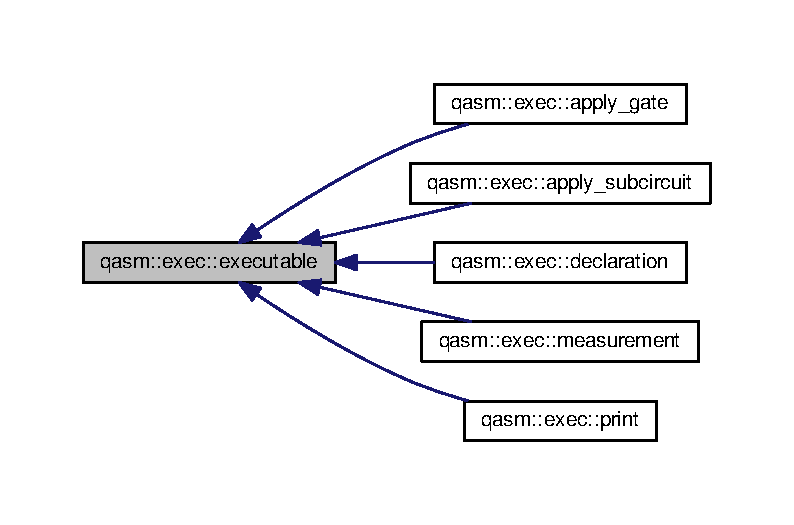
\includegraphics[width=350pt]{classqasm_1_1exec_1_1executable__inherit__graph}
\end{center}
\end{figure}
\subsection*{Public Member Functions}
\begin{DoxyCompactItemize}
\item 
virtual void \hyperlink{classqasm_1_1exec_1_1executable_ad07f864a889edb0777ebbb1bc1628121}{invoke\+\_\+rootprogram} (\hyperlink{classqasm_1_1runtime_1_1environment}{runtime\+::environment} \&env)
\item 
virtual void \hyperlink{classqasm_1_1exec_1_1executable_ad73a67bcb74196954455b45804944544}{invoke\+\_\+subprogram} (\hyperlink{classqasm_1_1runtime_1_1environment}{runtime\+::environment} \&env)
\end{DoxyCompactItemize}


\subsection{Detailed Description}
Represents an instruction that can be run 

\subsection{Member Function Documentation}
\index{qasm\+::exec\+::executable@{qasm\+::exec\+::executable}!invoke\+\_\+rootprogram@{invoke\+\_\+rootprogram}}
\index{invoke\+\_\+rootprogram@{invoke\+\_\+rootprogram}!qasm\+::exec\+::executable@{qasm\+::exec\+::executable}}
\subsubsection[{\texorpdfstring{invoke\+\_\+rootprogram(runtime\+::environment \&env)}{invoke_rootprogram(runtime::environment &env)}}]{\setlength{\rightskip}{0pt plus 5cm}virtual void qasm\+::exec\+::executable\+::invoke\+\_\+rootprogram (
\begin{DoxyParamCaption}
\item[{{\bf runtime\+::environment} \&}]{env}
\end{DoxyParamCaption}
)\hspace{0.3cm}{\ttfamily [inline]}, {\ttfamily [virtual]}}\hypertarget{classqasm_1_1exec_1_1executable_ad07f864a889edb0777ebbb1bc1628121}{}\label{classqasm_1_1exec_1_1executable_ad07f864a889edb0777ebbb1bc1628121}
Run instruction\textquotesingle{}s primary operation 

Reimplemented in \hyperlink{classqasm_1_1exec_1_1reset_ac23af0d0766e90a32de00446933e0eb6}{qasm\+::exec\+::reset}, \hyperlink{classqasm_1_1exec_1_1declaration_a4f1396fca212fb0ce984d2cea90df0a8}{qasm\+::exec\+::declaration}, \hyperlink{classqasm_1_1exec_1_1measurement_aefa96cf86f31c40a75fbc46924c94bb8}{qasm\+::exec\+::measurement}, \hyperlink{classqasm_1_1exec_1_1print_ae803c9f70d2a1afd3bbe6e0520e9678b}{qasm\+::exec\+::print}, and \hyperlink{classqasm_1_1exec_1_1apply__gate_a4ab94a7feee1830b4be52a487e9cdef5}{qasm\+::exec\+::apply\+\_\+gate}.

\index{qasm\+::exec\+::executable@{qasm\+::exec\+::executable}!invoke\+\_\+subprogram@{invoke\+\_\+subprogram}}
\index{invoke\+\_\+subprogram@{invoke\+\_\+subprogram}!qasm\+::exec\+::executable@{qasm\+::exec\+::executable}}
\subsubsection[{\texorpdfstring{invoke\+\_\+subprogram(runtime\+::environment \&env)}{invoke_subprogram(runtime::environment &env)}}]{\setlength{\rightskip}{0pt plus 5cm}virtual void qasm\+::exec\+::executable\+::invoke\+\_\+subprogram (
\begin{DoxyParamCaption}
\item[{{\bf runtime\+::environment} \&}]{env}
\end{DoxyParamCaption}
)\hspace{0.3cm}{\ttfamily [inline]}, {\ttfamily [virtual]}}\hypertarget{classqasm_1_1exec_1_1executable_ad73a67bcb74196954455b45804944544}{}\label{classqasm_1_1exec_1_1executable_ad73a67bcb74196954455b45804944544}
Run instruction\textquotesingle{}s secondary operation 

The documentation for this class was generated from the following file\+:\begin{DoxyCompactItemize}
\item 
src/runtime/\hyperlink{runtime_8hpp}{runtime.\+hpp}\end{DoxyCompactItemize}

\hypertarget{classqlib_1_1ide_1_1FileManager}{}\section{qlib.\+ide.\+File\+Manager Class Reference}
\label{classqlib_1_1ide_1_1FileManager}\index{qlib.\+ide.\+File\+Manager@{qlib.\+ide.\+File\+Manager}}


Collaboration diagram for qlib.\+ide.\+File\+Manager\+:\nopagebreak
\begin{figure}[H]
\begin{center}
\leavevmode
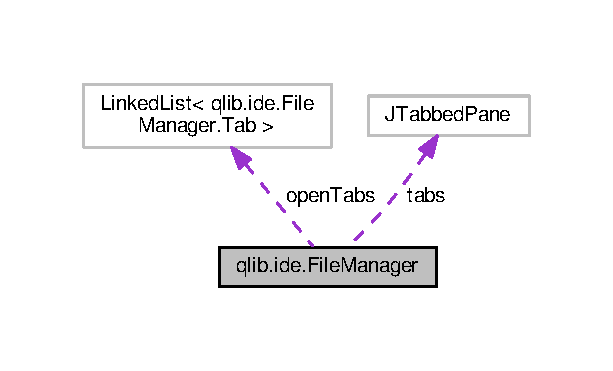
\includegraphics[width=294pt]{classqlib_1_1ide_1_1FileManager__coll__graph}
\end{center}
\end{figure}
\subsection*{Classes}
\begin{DoxyCompactItemize}
\item 
class \hyperlink{classqlib_1_1ide_1_1FileManager_1_1Tab}{Tab}
\end{DoxyCompactItemize}
\subsection*{Public Member Functions}
\begin{DoxyCompactItemize}
\item 
\hyperlink{classqlib_1_1ide_1_1FileManager_ad6a89c4b0f958a34dd7450ab8826f647}{File\+Manager} ()
\item 
void \hyperlink{classqlib_1_1ide_1_1FileManager_a9b6923afb970442de71a07405abc6751}{empty} ()
\item 
void \hyperlink{classqlib_1_1ide_1_1FileManager_a1a740e6ad8726d1caad504a4b7a53859}{open} (String file)
\item 
void \hyperlink{classqlib_1_1ide_1_1FileManager_a043ddff761f62666fa4f6959b7e116c3}{save} ()
\item 
void \hyperlink{classqlib_1_1ide_1_1FileManager_acefb35297452dccb1f7a2cbebd08b0fc}{close} ()
\item 
File \hyperlink{classqlib_1_1ide_1_1FileManager_afa5d713317aa1248f7c102dd086e53b8}{get\+Active} ()
\item 
J\+Tabbed\+Pane \hyperlink{classqlib_1_1ide_1_1FileManager_a986392eebf1b4d6df69bf3eca688d926}{get\+Panel} ()
\end{DoxyCompactItemize}
\subsection*{Private Attributes}
\begin{DoxyCompactItemize}
\item 
J\+Tabbed\+Pane \hyperlink{classqlib_1_1ide_1_1FileManager_ad30cb7a3ba1310ab8cb38f11bb84f0c1}{tabs}
\item 
Linked\+List$<$ \hyperlink{classqlib_1_1ide_1_1FileManager_1_1Tab}{Tab} $>$ \hyperlink{classqlib_1_1ide_1_1FileManager_af28dcef61bad9a512d4dfba62d9288a3}{open\+Tabs} = new Linked\+List$<$\hyperlink{classqlib_1_1ide_1_1FileManager_1_1Tab}{Tab}$>$()
\end{DoxyCompactItemize}


\subsection{Detailed Description}
Class for managing files and tabs in the I\+DE \begin{DoxyAuthor}{Author}
halse 
\end{DoxyAuthor}


\subsection{Constructor \& Destructor Documentation}
\index{qlib\+::ide\+::\+File\+Manager@{qlib\+::ide\+::\+File\+Manager}!File\+Manager@{File\+Manager}}
\index{File\+Manager@{File\+Manager}!qlib\+::ide\+::\+File\+Manager@{qlib\+::ide\+::\+File\+Manager}}
\subsubsection[{\texorpdfstring{File\+Manager()}{FileManager()}}]{\setlength{\rightskip}{0pt plus 5cm}qlib.\+ide.\+File\+Manager.\+File\+Manager (
\begin{DoxyParamCaption}
{}
\end{DoxyParamCaption}
)\hspace{0.3cm}{\ttfamily [inline]}}\hypertarget{classqlib_1_1ide_1_1FileManager_ad6a89c4b0f958a34dd7450ab8826f647}{}\label{classqlib_1_1ide_1_1FileManager_ad6a89c4b0f958a34dd7450ab8826f647}
Create a file manager 

\subsection{Member Function Documentation}
\index{qlib\+::ide\+::\+File\+Manager@{qlib\+::ide\+::\+File\+Manager}!close@{close}}
\index{close@{close}!qlib\+::ide\+::\+File\+Manager@{qlib\+::ide\+::\+File\+Manager}}
\subsubsection[{\texorpdfstring{close()}{close()}}]{\setlength{\rightskip}{0pt plus 5cm}void qlib.\+ide.\+File\+Manager.\+close (
\begin{DoxyParamCaption}
{}
\end{DoxyParamCaption}
)\hspace{0.3cm}{\ttfamily [inline]}}\hypertarget{classqlib_1_1ide_1_1FileManager_acefb35297452dccb1f7a2cbebd08b0fc}{}\label{classqlib_1_1ide_1_1FileManager_acefb35297452dccb1f7a2cbebd08b0fc}
Close the current file \index{qlib\+::ide\+::\+File\+Manager@{qlib\+::ide\+::\+File\+Manager}!empty@{empty}}
\index{empty@{empty}!qlib\+::ide\+::\+File\+Manager@{qlib\+::ide\+::\+File\+Manager}}
\subsubsection[{\texorpdfstring{empty()}{empty()}}]{\setlength{\rightskip}{0pt plus 5cm}void qlib.\+ide.\+File\+Manager.\+empty (
\begin{DoxyParamCaption}
{}
\end{DoxyParamCaption}
)\hspace{0.3cm}{\ttfamily [inline]}}\hypertarget{classqlib_1_1ide_1_1FileManager_a9b6923afb970442de71a07405abc6751}{}\label{classqlib_1_1ide_1_1FileManager_a9b6923afb970442de71a07405abc6751}
Create an empty file \index{qlib\+::ide\+::\+File\+Manager@{qlib\+::ide\+::\+File\+Manager}!get\+Active@{get\+Active}}
\index{get\+Active@{get\+Active}!qlib\+::ide\+::\+File\+Manager@{qlib\+::ide\+::\+File\+Manager}}
\subsubsection[{\texorpdfstring{get\+Active()}{getActive()}}]{\setlength{\rightskip}{0pt plus 5cm}File qlib.\+ide.\+File\+Manager.\+get\+Active (
\begin{DoxyParamCaption}
{}
\end{DoxyParamCaption}
)\hspace{0.3cm}{\ttfamily [inline]}}\hypertarget{classqlib_1_1ide_1_1FileManager_afa5d713317aa1248f7c102dd086e53b8}{}\label{classqlib_1_1ide_1_1FileManager_afa5d713317aa1248f7c102dd086e53b8}
Get the current file \begin{DoxyReturn}{Returns}

\end{DoxyReturn}
\index{qlib\+::ide\+::\+File\+Manager@{qlib\+::ide\+::\+File\+Manager}!get\+Panel@{get\+Panel}}
\index{get\+Panel@{get\+Panel}!qlib\+::ide\+::\+File\+Manager@{qlib\+::ide\+::\+File\+Manager}}
\subsubsection[{\texorpdfstring{get\+Panel()}{getPanel()}}]{\setlength{\rightskip}{0pt plus 5cm}J\+Tabbed\+Pane qlib.\+ide.\+File\+Manager.\+get\+Panel (
\begin{DoxyParamCaption}
{}
\end{DoxyParamCaption}
)\hspace{0.3cm}{\ttfamily [inline]}}\hypertarget{classqlib_1_1ide_1_1FileManager_a986392eebf1b4d6df69bf3eca688d926}{}\label{classqlib_1_1ide_1_1FileManager_a986392eebf1b4d6df69bf3eca688d926}
Get the internal reference to the tabbed panel \begin{DoxyReturn}{Returns}

\end{DoxyReturn}
\index{qlib\+::ide\+::\+File\+Manager@{qlib\+::ide\+::\+File\+Manager}!open@{open}}
\index{open@{open}!qlib\+::ide\+::\+File\+Manager@{qlib\+::ide\+::\+File\+Manager}}
\subsubsection[{\texorpdfstring{open(\+String file)}{open(String file)}}]{\setlength{\rightskip}{0pt plus 5cm}void qlib.\+ide.\+File\+Manager.\+open (
\begin{DoxyParamCaption}
\item[{String}]{file}
\end{DoxyParamCaption}
)\hspace{0.3cm}{\ttfamily [inline]}}\hypertarget{classqlib_1_1ide_1_1FileManager_a1a740e6ad8726d1caad504a4b7a53859}{}\label{classqlib_1_1ide_1_1FileManager_a1a740e6ad8726d1caad504a4b7a53859}
Open a file in the editor 
\begin{DoxyParams}{Parameters}
{\em file} & \\
\hline
\end{DoxyParams}
\index{qlib\+::ide\+::\+File\+Manager@{qlib\+::ide\+::\+File\+Manager}!save@{save}}
\index{save@{save}!qlib\+::ide\+::\+File\+Manager@{qlib\+::ide\+::\+File\+Manager}}
\subsubsection[{\texorpdfstring{save()}{save()}}]{\setlength{\rightskip}{0pt plus 5cm}void qlib.\+ide.\+File\+Manager.\+save (
\begin{DoxyParamCaption}
{}
\end{DoxyParamCaption}
)\hspace{0.3cm}{\ttfamily [inline]}}\hypertarget{classqlib_1_1ide_1_1FileManager_a043ddff761f62666fa4f6959b7e116c3}{}\label{classqlib_1_1ide_1_1FileManager_a043ddff761f62666fa4f6959b7e116c3}
Save the current file 

\subsection{Member Data Documentation}
\index{qlib\+::ide\+::\+File\+Manager@{qlib\+::ide\+::\+File\+Manager}!open\+Tabs@{open\+Tabs}}
\index{open\+Tabs@{open\+Tabs}!qlib\+::ide\+::\+File\+Manager@{qlib\+::ide\+::\+File\+Manager}}
\subsubsection[{\texorpdfstring{open\+Tabs}{openTabs}}]{\setlength{\rightskip}{0pt plus 5cm}Linked\+List$<${\bf Tab}$>$ qlib.\+ide.\+File\+Manager.\+open\+Tabs = new Linked\+List$<${\bf Tab}$>$()\hspace{0.3cm}{\ttfamily [private]}}\hypertarget{classqlib_1_1ide_1_1FileManager_af28dcef61bad9a512d4dfba62d9288a3}{}\label{classqlib_1_1ide_1_1FileManager_af28dcef61bad9a512d4dfba62d9288a3}
List of tab data \index{qlib\+::ide\+::\+File\+Manager@{qlib\+::ide\+::\+File\+Manager}!tabs@{tabs}}
\index{tabs@{tabs}!qlib\+::ide\+::\+File\+Manager@{qlib\+::ide\+::\+File\+Manager}}
\subsubsection[{\texorpdfstring{tabs}{tabs}}]{\setlength{\rightskip}{0pt plus 5cm}J\+Tabbed\+Pane qlib.\+ide.\+File\+Manager.\+tabs\hspace{0.3cm}{\ttfamily [private]}}\hypertarget{classqlib_1_1ide_1_1FileManager_ad30cb7a3ba1310ab8cb38f11bb84f0c1}{}\label{classqlib_1_1ide_1_1FileManager_ad30cb7a3ba1310ab8cb38f11bb84f0c1}
Internal reference to a tabbed panel 

The documentation for this class was generated from the following file\+:\begin{DoxyCompactItemize}
\item 
src/ide/src/qlib/ide/\hyperlink{FileManager_8java}{File\+Manager.\+java}\end{DoxyCompactItemize}

\hypertarget{classqlib_1_1quantum_1_1gates_1_1igate}{}\section{qlib\+:\+:quantum\+:\+:gates\+:\+:igate Class Reference}
\label{classqlib_1_1quantum_1_1gates_1_1igate}\index{qlib\+::quantum\+::gates\+::igate@{qlib\+::quantum\+::gates\+::igate}}


{\ttfamily \#include $<$igate.\+hpp$>$}



Inheritance diagram for qlib\+:\+:quantum\+:\+:gates\+:\+:igate\+:
\nopagebreak
\begin{figure}[H]
\begin{center}
\leavevmode
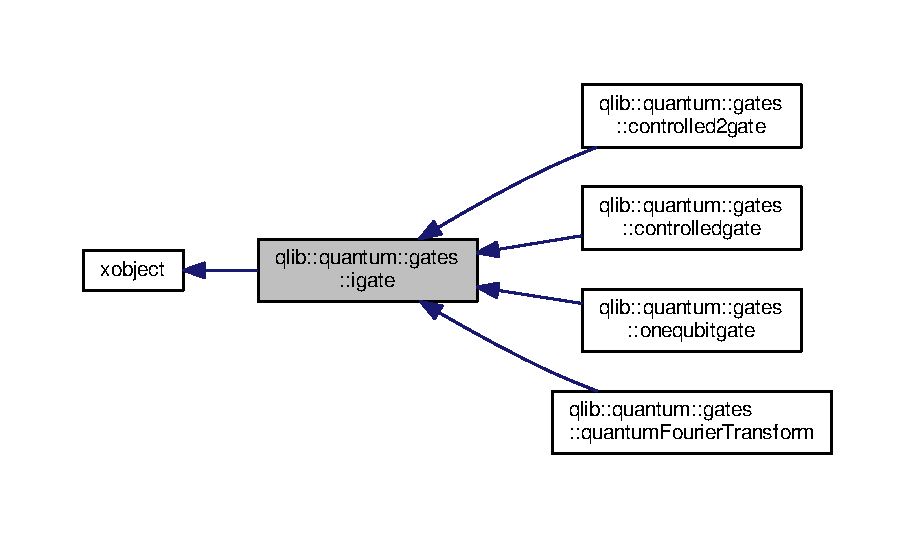
\includegraphics[width=350pt]{classqlib_1_1quantum_1_1gates_1_1igate__inherit__graph}
\end{center}
\end{figure}


Collaboration diagram for qlib\+:\+:quantum\+:\+:gates\+:\+:igate\+:\nopagebreak
\begin{figure}[H]
\begin{center}
\leavevmode
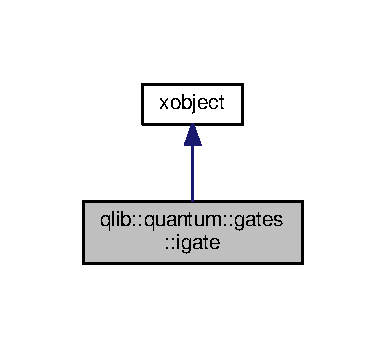
\includegraphics[width=185pt]{classqlib_1_1quantum_1_1gates_1_1igate__coll__graph}
\end{center}
\end{figure}
\subsection*{Public Member Functions}
\begin{DoxyCompactItemize}
\item 
virtual \hyperlink{classqlib_1_1quantum_1_1gates_1_1igate_afa0161a395344bb7765b61fbf94d01b5}{$\sim$igate} ()
\item 
virtual std\+::string \hyperlink{classqlib_1_1quantum_1_1gates_1_1igate_ae8f8dda69d7742c12c743829abb3662b}{name} ()=0
\item 
virtual size\+\_\+t \hyperlink{classqlib_1_1quantum_1_1gates_1_1igate_ac8aa56b0095a94fdd437bc55d90aec9d}{inputs} ()=0
\item 
virtual void \hyperlink{classqlib_1_1quantum_1_1gates_1_1igate_a66038ee65fec12c627789505e11f1e23}{operate} (\hyperlink{classqlib_1_1math_1_1matrix}{matrix} \&in, \hyperlink{classqlib_1_1math_1_1matrix}{matrix} \&out, std\+::vector$<$ u64 $>$ input\+Qubits)=0
\end{DoxyCompactItemize}
\subsection*{Static Public Member Functions}
\begin{DoxyCompactItemize}
\item 
static bool \hyperlink{classqlib_1_1quantum_1_1gates_1_1igate_ab69530a50a6b78e429abe3c08407b222}{is\+Gateable} (\hyperlink{classqlib_1_1math_1_1matrix}{matrix} \&a)
\end{DoxyCompactItemize}


\subsection{Constructor \& Destructor Documentation}
\index{qlib\+::quantum\+::gates\+::igate@{qlib\+::quantum\+::gates\+::igate}!````~igate@{$\sim$igate}}
\index{````~igate@{$\sim$igate}!qlib\+::quantum\+::gates\+::igate@{qlib\+::quantum\+::gates\+::igate}}
\subsubsection[{\texorpdfstring{$\sim$igate()}{~igate()}}]{\setlength{\rightskip}{0pt plus 5cm}virtual qlib\+::quantum\+::gates\+::igate\+::$\sim$igate (
\begin{DoxyParamCaption}
{}
\end{DoxyParamCaption}
)\hspace{0.3cm}{\ttfamily [inline]}, {\ttfamily [virtual]}}\hypertarget{classqlib_1_1quantum_1_1gates_1_1igate_afa0161a395344bb7765b61fbf94d01b5}{}\label{classqlib_1_1quantum_1_1gates_1_1igate_afa0161a395344bb7765b61fbf94d01b5}
Virtual destrutor, overwritten by subclasses 

\subsection{Member Function Documentation}
\index{qlib\+::quantum\+::gates\+::igate@{qlib\+::quantum\+::gates\+::igate}!inputs@{inputs}}
\index{inputs@{inputs}!qlib\+::quantum\+::gates\+::igate@{qlib\+::quantum\+::gates\+::igate}}
\subsubsection[{\texorpdfstring{inputs()=0}{inputs()=0}}]{\setlength{\rightskip}{0pt plus 5cm}virtual size\+\_\+t qlib\+::quantum\+::gates\+::igate\+::inputs (
\begin{DoxyParamCaption}
{}
\end{DoxyParamCaption}
)\hspace{0.3cm}{\ttfamily [pure virtual]}}\hypertarget{classqlib_1_1quantum_1_1gates_1_1igate_ac8aa56b0095a94fdd437bc55d90aec9d}{}\label{classqlib_1_1quantum_1_1gates_1_1igate_ac8aa56b0095a94fdd437bc55d90aec9d}


Implemented in \hyperlink{classqlib_1_1quantum_1_1gates_1_1quantumFourierTransform_a08ee18ae7b516c2f77d1f864a010856f}{qlib\+::quantum\+::gates\+::quantum\+Fourier\+Transform}, \hyperlink{classqlib_1_1quantum_1_1gates_1_1onequbitgate_a050ed71ebff89050c3123124f8ba8719}{qlib\+::quantum\+::gates\+::onequbitgate}, \hyperlink{classqlib_1_1quantum_1_1gates_1_1controlled2gate_a27a8793a3015aa9797f03fa0174113c2}{qlib\+::quantum\+::gates\+::controlled2gate}, and \hyperlink{classqlib_1_1quantum_1_1gates_1_1controlledgate_adb544cb10cd5f8836e331102f7c7e9d6}{qlib\+::quantum\+::gates\+::controlledgate}.

\index{qlib\+::quantum\+::gates\+::igate@{qlib\+::quantum\+::gates\+::igate}!is\+Gateable@{is\+Gateable}}
\index{is\+Gateable@{is\+Gateable}!qlib\+::quantum\+::gates\+::igate@{qlib\+::quantum\+::gates\+::igate}}
\subsubsection[{\texorpdfstring{is\+Gateable(matrix \&a)}{isGateable(matrix &a)}}]{\setlength{\rightskip}{0pt plus 5cm}static bool qlib\+::quantum\+::gates\+::igate\+::is\+Gateable (
\begin{DoxyParamCaption}
\item[{{\bf matrix} \&}]{a}
\end{DoxyParamCaption}
)\hspace{0.3cm}{\ttfamily [inline]}, {\ttfamily [static]}}\hypertarget{classqlib_1_1quantum_1_1gates_1_1igate_ab69530a50a6b78e429abe3c08407b222}{}\label{classqlib_1_1quantum_1_1gates_1_1igate_ab69530a50a6b78e429abe3c08407b222}
Test if a given matrix matches quantum gate specifications (square \& unitary) \index{qlib\+::quantum\+::gates\+::igate@{qlib\+::quantum\+::gates\+::igate}!name@{name}}
\index{name@{name}!qlib\+::quantum\+::gates\+::igate@{qlib\+::quantum\+::gates\+::igate}}
\subsubsection[{\texorpdfstring{name()=0}{name()=0}}]{\setlength{\rightskip}{0pt plus 5cm}virtual std\+::string qlib\+::quantum\+::gates\+::igate\+::name (
\begin{DoxyParamCaption}
{}
\end{DoxyParamCaption}
)\hspace{0.3cm}{\ttfamily [pure virtual]}}\hypertarget{classqlib_1_1quantum_1_1gates_1_1igate_ae8f8dda69d7742c12c743829abb3662b}{}\label{classqlib_1_1quantum_1_1gates_1_1igate_ae8f8dda69d7742c12c743829abb3662b}


Implemented in \hyperlink{classqlib_1_1quantum_1_1gates_1_1onequbitgate_aacf3878010f0c1327bae4dcc7faf4c92}{qlib\+::quantum\+::gates\+::onequbitgate}, \hyperlink{classqlib_1_1quantum_1_1gates_1_1controlled2gate_a25121d9bc52a594a718b6d8037ea6cc0}{qlib\+::quantum\+::gates\+::controlled2gate}, \hyperlink{classqlib_1_1quantum_1_1gates_1_1controlledgate_a7fb8875c83106b35d733cc96b312b957}{qlib\+::quantum\+::gates\+::controlledgate}, and \hyperlink{classqlib_1_1quantum_1_1gates_1_1quantumFourierTransform_a28d08c879986bbf22846ada13f861781}{qlib\+::quantum\+::gates\+::quantum\+Fourier\+Transform}.

\index{qlib\+::quantum\+::gates\+::igate@{qlib\+::quantum\+::gates\+::igate}!operate@{operate}}
\index{operate@{operate}!qlib\+::quantum\+::gates\+::igate@{qlib\+::quantum\+::gates\+::igate}}
\subsubsection[{\texorpdfstring{operate(matrix \&in, matrix \&out, std\+::vector$<$ u64 $>$ input\+Qubits)=0}{operate(matrix &in, matrix &out, std::vector< u64 > inputQubits)=0}}]{\setlength{\rightskip}{0pt plus 5cm}virtual void qlib\+::quantum\+::gates\+::igate\+::operate (
\begin{DoxyParamCaption}
\item[{{\bf matrix} \&}]{in, }
\item[{{\bf matrix} \&}]{out, }
\item[{std\+::vector$<$ u64 $>$}]{input\+Qubits}
\end{DoxyParamCaption}
)\hspace{0.3cm}{\ttfamily [pure virtual]}}\hypertarget{classqlib_1_1quantum_1_1gates_1_1igate_a66038ee65fec12c627789505e11f1e23}{}\label{classqlib_1_1quantum_1_1gates_1_1igate_a66038ee65fec12c627789505e11f1e23}


Implemented in \hyperlink{classqlib_1_1quantum_1_1gates_1_1onequbitgate_a280c7a7d29032eeb95afcb3d6668e7db}{qlib\+::quantum\+::gates\+::onequbitgate}, \hyperlink{classqlib_1_1quantum_1_1gates_1_1controlled2gate_a272635da6a7b8f65379f6ecb42df9389}{qlib\+::quantum\+::gates\+::controlled2gate}, \hyperlink{classqlib_1_1quantum_1_1gates_1_1controlledgate_aec6e423cc6ae442c5c3c5dc04581959e}{qlib\+::quantum\+::gates\+::controlledgate}, and \hyperlink{classqlib_1_1quantum_1_1gates_1_1quantumFourierTransform_a81c62ab7b1edeeb2b01d5f9dacca2bae}{qlib\+::quantum\+::gates\+::quantum\+Fourier\+Transform}.



The documentation for this class was generated from the following file\+:\begin{DoxyCompactItemize}
\item 
src/core/quantum/gates/\hyperlink{igate_8hpp}{igate.\+hpp}\end{DoxyCompactItemize}

\hypertarget{classqasm_1_1exec_1_1import}{}\section{qasm\+:\+:exec\+:\+:import Class Reference}
\label{classqasm_1_1exec_1_1import}\index{qasm\+::exec\+::import@{qasm\+::exec\+::import}}


{\ttfamily \#include $<$runtime.\+hpp$>$}



Inheritance diagram for qasm\+:\+:exec\+:\+:import\+:
\nopagebreak
\begin{figure}[H]
\begin{center}
\leavevmode
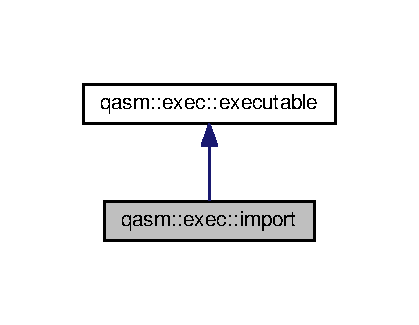
\includegraphics[width=201pt]{classqasm_1_1exec_1_1import__inherit__graph}
\end{center}
\end{figure}


Collaboration diagram for qasm\+:\+:exec\+:\+:import\+:
\nopagebreak
\begin{figure}[H]
\begin{center}
\leavevmode
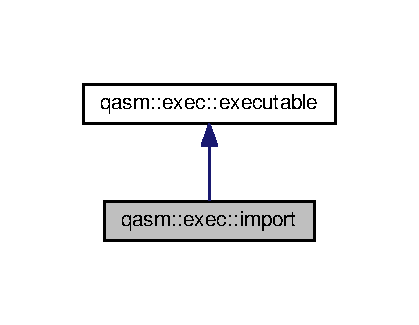
\includegraphics[width=201pt]{classqasm_1_1exec_1_1import__coll__graph}
\end{center}
\end{figure}
\subsection*{Public Member Functions}
\begin{DoxyCompactItemize}
\item 
\hyperlink{classqasm_1_1exec_1_1import_a95ac5a6910c5820c41314dc4de5dd98a}{import} (string file)
\end{DoxyCompactItemize}
\subsection*{Public Attributes}
\begin{DoxyCompactItemize}
\item 
string \hyperlink{classqasm_1_1exec_1_1import_a421f281a62fa921c13a3fc86d6c6fa17}{filename}
\end{DoxyCompactItemize}


\subsection{Detailed Description}
Instruction to import a file 

\subsection{Constructor \& Destructor Documentation}
\index{qasm\+::exec\+::import@{qasm\+::exec\+::import}!import@{import}}
\index{import@{import}!qasm\+::exec\+::import@{qasm\+::exec\+::import}}
\subsubsection[{\texorpdfstring{import(string file)}{import(string file)}}]{\setlength{\rightskip}{0pt plus 5cm}qasm\+::exec\+::import\+::import (
\begin{DoxyParamCaption}
\item[{string}]{file}
\end{DoxyParamCaption}
)\hspace{0.3cm}{\ttfamily [inline]}}\hypertarget{classqasm_1_1exec_1_1import_a95ac5a6910c5820c41314dc4de5dd98a}{}\label{classqasm_1_1exec_1_1import_a95ac5a6910c5820c41314dc4de5dd98a}


\subsection{Member Data Documentation}
\index{qasm\+::exec\+::import@{qasm\+::exec\+::import}!filename@{filename}}
\index{filename@{filename}!qasm\+::exec\+::import@{qasm\+::exec\+::import}}
\subsubsection[{\texorpdfstring{filename}{filename}}]{\setlength{\rightskip}{0pt plus 5cm}string qasm\+::exec\+::import\+::filename}\hypertarget{classqasm_1_1exec_1_1import_a421f281a62fa921c13a3fc86d6c6fa17}{}\label{classqasm_1_1exec_1_1import_a421f281a62fa921c13a3fc86d6c6fa17}


The documentation for this class was generated from the following file\+:\begin{DoxyCompactItemize}
\item 
src/runtime/\hyperlink{runtime_8hpp}{runtime.\+hpp}\end{DoxyCompactItemize}

\hypertarget{classqlib_1_1ide_1_1IniIO}{}\section{qlib.\+ide.\+Ini\+IO Class Reference}
\label{classqlib_1_1ide_1_1IniIO}\index{qlib.\+ide.\+Ini\+IO@{qlib.\+ide.\+Ini\+IO}}


Inheritance diagram for qlib.\+ide.\+Ini\+IO\+:\nopagebreak
\begin{figure}[H]
\begin{center}
\leavevmode
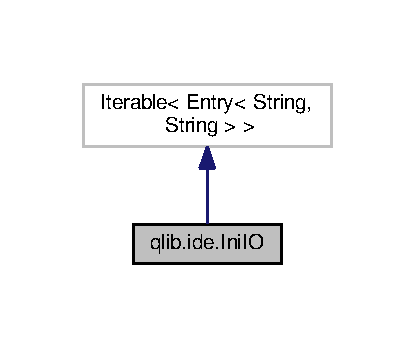
\includegraphics[width=199pt]{classqlib_1_1ide_1_1IniIO__inherit__graph}
\end{center}
\end{figure}


Collaboration diagram for qlib.\+ide.\+Ini\+IO\+:\nopagebreak
\begin{figure}[H]
\begin{center}
\leavevmode
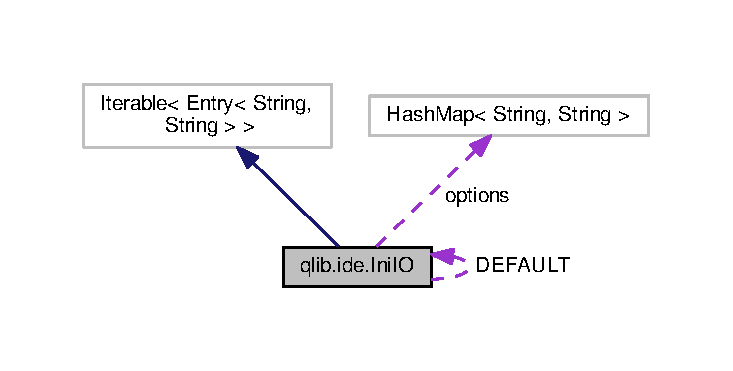
\includegraphics[width=350pt]{classqlib_1_1ide_1_1IniIO__coll__graph}
\end{center}
\end{figure}
\subsection*{Public Member Functions}
\begin{DoxyCompactItemize}
\item 
boolean \hyperlink{classqlib_1_1ide_1_1IniIO_a69a0c6a7e4bf6d161e37db728bff03a6}{is\+Set} (String prop)
\item 
String \hyperlink{classqlib_1_1ide_1_1IniIO_aab6608976c5f371d0f044fc7d39f0328}{get\+String} (String prop)
\item 
Integer \hyperlink{classqlib_1_1ide_1_1IniIO_a01a6fe06552fefab11669ea65ace7392}{get\+Int} (String prop)
\item 
void \hyperlink{classqlib_1_1ide_1_1IniIO_a2337d52ad4d343c74b808f64e70710f0}{set} (String prop, Object value)
\item 
boolean \hyperlink{classqlib_1_1ide_1_1IniIO_a68567b380e0074a223137077125eb060}{exists} (String prop)
\item 
void \hyperlink{classqlib_1_1ide_1_1IniIO_a586ba8be1bf5be1d406c75da8a99464f}{clear} ()
\item 
Iterator$<$ Entry$<$ String, String $>$ $>$ \hyperlink{classqlib_1_1ide_1_1IniIO_a51efa19f17cc902c47b577d39177172f}{iterator} ()
\end{DoxyCompactItemize}
\subsection*{Static Public Member Functions}
\begin{DoxyCompactItemize}
\item 
static \hyperlink{classqlib_1_1ide_1_1IniIO}{Ini\+IO} \hyperlink{classqlib_1_1ide_1_1IniIO_a02df232b5337879896c1e067b6e27601}{template} (String\mbox{[}$\,$\mbox{]} Key\+Value\+Pairs)
\item 
static \hyperlink{classqlib_1_1ide_1_1IniIO}{Ini\+IO} \hyperlink{classqlib_1_1ide_1_1IniIO_ae79dc4c2b69222d0e1725e70406da4c6}{read} (String filename)
\item 
static \hyperlink{classqlib_1_1ide_1_1IniIO}{Ini\+IO} \hyperlink{classqlib_1_1ide_1_1IniIO_aa8afcd3e7f28ea7d5324ab186650be1d}{merge} (\hyperlink{classqlib_1_1ide_1_1IniIO}{Ini\+IO} a, \hyperlink{classqlib_1_1ide_1_1IniIO}{Ini\+IO} b)
\item 
static \hyperlink{classqlib_1_1ide_1_1IniIO}{Ini\+IO} \hyperlink{classqlib_1_1ide_1_1IniIO_a25c322821c43bb710404a05210fb20be}{read\+And\+Update} (String fname, \hyperlink{classqlib_1_1ide_1_1IniIO}{Ini\+IO} update\+Template)
\item 
static void \hyperlink{classqlib_1_1ide_1_1IniIO_a10bafd582cb3816d23c93f1883b3e68b}{write} (\hyperlink{classqlib_1_1ide_1_1IniIO}{Ini\+IO} settings, String filename)
\end{DoxyCompactItemize}
\subsection*{Static Public Attributes}
\begin{DoxyCompactItemize}
\item 
static \hyperlink{classqlib_1_1ide_1_1IniIO}{Ini\+IO} \hyperlink{classqlib_1_1ide_1_1IniIO_a632b3fd3f02261c98a2aecf793c956a5}{D\+E\+F\+A\+U\+LT}
\end{DoxyCompactItemize}
\subsection*{Private Member Functions}
\begin{DoxyCompactItemize}
\item 
\hyperlink{classqlib_1_1ide_1_1IniIO_a0eadd42f5485d6bff447436734eda253}{Ini\+IO} ()
\end{DoxyCompactItemize}
\subsection*{Private Attributes}
\begin{DoxyCompactItemize}
\item 
Hash\+Map$<$ String, String $>$ \hyperlink{classqlib_1_1ide_1_1IniIO_a8676d10eea865975fca03579a63b9831}{options} = new Hash\+Map$<$String,String$>$()
\end{DoxyCompactItemize}


\subsection{Detailed Description}
Class for storing I\+NI type config information \begin{DoxyAuthor}{Author}
Colin Halseth 
\end{DoxyAuthor}


\subsection{Constructor \& Destructor Documentation}
\index{qlib\+::ide\+::\+Ini\+IO@{qlib\+::ide\+::\+Ini\+IO}!Ini\+IO@{Ini\+IO}}
\index{Ini\+IO@{Ini\+IO}!qlib\+::ide\+::\+Ini\+IO@{qlib\+::ide\+::\+Ini\+IO}}
\subsubsection[{\texorpdfstring{Ini\+I\+O()}{IniIO()}}]{\setlength{\rightskip}{0pt plus 5cm}qlib.\+ide.\+Ini\+I\+O.\+Ini\+IO (
\begin{DoxyParamCaption}
{}
\end{DoxyParamCaption}
)\hspace{0.3cm}{\ttfamily [inline]}, {\ttfamily [private]}}\hypertarget{classqlib_1_1ide_1_1IniIO_a0eadd42f5485d6bff447436734eda253}{}\label{classqlib_1_1ide_1_1IniIO_a0eadd42f5485d6bff447436734eda253}
Create an empty config file 

\subsection{Member Function Documentation}
\index{qlib\+::ide\+::\+Ini\+IO@{qlib\+::ide\+::\+Ini\+IO}!clear@{clear}}
\index{clear@{clear}!qlib\+::ide\+::\+Ini\+IO@{qlib\+::ide\+::\+Ini\+IO}}
\subsubsection[{\texorpdfstring{clear()}{clear()}}]{\setlength{\rightskip}{0pt plus 5cm}void qlib.\+ide.\+Ini\+I\+O.\+clear (
\begin{DoxyParamCaption}
{}
\end{DoxyParamCaption}
)\hspace{0.3cm}{\ttfamily [inline]}}\hypertarget{classqlib_1_1ide_1_1IniIO_a586ba8be1bf5be1d406c75da8a99464f}{}\label{classqlib_1_1ide_1_1IniIO_a586ba8be1bf5be1d406c75da8a99464f}
Remove all config options \index{qlib\+::ide\+::\+Ini\+IO@{qlib\+::ide\+::\+Ini\+IO}!exists@{exists}}
\index{exists@{exists}!qlib\+::ide\+::\+Ini\+IO@{qlib\+::ide\+::\+Ini\+IO}}
\subsubsection[{\texorpdfstring{exists(\+String prop)}{exists(String prop)}}]{\setlength{\rightskip}{0pt plus 5cm}boolean qlib.\+ide.\+Ini\+I\+O.\+exists (
\begin{DoxyParamCaption}
\item[{String}]{prop}
\end{DoxyParamCaption}
)\hspace{0.3cm}{\ttfamily [inline]}}\hypertarget{classqlib_1_1ide_1_1IniIO_a68567b380e0074a223137077125eb060}{}\label{classqlib_1_1ide_1_1IniIO_a68567b380e0074a223137077125eb060}
Check if a property exists in the config 
\begin{DoxyParams}{Parameters}
{\em prop} & \\
\hline
\end{DoxyParams}
\begin{DoxyReturn}{Returns}

\end{DoxyReturn}
\index{qlib\+::ide\+::\+Ini\+IO@{qlib\+::ide\+::\+Ini\+IO}!get\+Int@{get\+Int}}
\index{get\+Int@{get\+Int}!qlib\+::ide\+::\+Ini\+IO@{qlib\+::ide\+::\+Ini\+IO}}
\subsubsection[{\texorpdfstring{get\+Int(\+String prop)}{getInt(String prop)}}]{\setlength{\rightskip}{0pt plus 5cm}Integer qlib.\+ide.\+Ini\+I\+O.\+get\+Int (
\begin{DoxyParamCaption}
\item[{String}]{prop}
\end{DoxyParamCaption}
)\hspace{0.3cm}{\ttfamily [inline]}}\hypertarget{classqlib_1_1ide_1_1IniIO_a01a6fe06552fefab11669ea65ace7392}{}\label{classqlib_1_1ide_1_1IniIO_a01a6fe06552fefab11669ea65ace7392}
Parse an integer from a named property 
\begin{DoxyParams}{Parameters}
{\em prop} & \\
\hline
\end{DoxyParams}
\begin{DoxyReturn}{Returns}

\end{DoxyReturn}
\index{qlib\+::ide\+::\+Ini\+IO@{qlib\+::ide\+::\+Ini\+IO}!get\+String@{get\+String}}
\index{get\+String@{get\+String}!qlib\+::ide\+::\+Ini\+IO@{qlib\+::ide\+::\+Ini\+IO}}
\subsubsection[{\texorpdfstring{get\+String(\+String prop)}{getString(String prop)}}]{\setlength{\rightskip}{0pt plus 5cm}String qlib.\+ide.\+Ini\+I\+O.\+get\+String (
\begin{DoxyParamCaption}
\item[{String}]{prop}
\end{DoxyParamCaption}
)\hspace{0.3cm}{\ttfamily [inline]}}\hypertarget{classqlib_1_1ide_1_1IniIO_aab6608976c5f371d0f044fc7d39f0328}{}\label{classqlib_1_1ide_1_1IniIO_aab6608976c5f371d0f044fc7d39f0328}
Get a string from a named property 
\begin{DoxyParams}{Parameters}
{\em prop} & \\
\hline
\end{DoxyParams}
\begin{DoxyReturn}{Returns}

\end{DoxyReturn}
\index{qlib\+::ide\+::\+Ini\+IO@{qlib\+::ide\+::\+Ini\+IO}!is\+Set@{is\+Set}}
\index{is\+Set@{is\+Set}!qlib\+::ide\+::\+Ini\+IO@{qlib\+::ide\+::\+Ini\+IO}}
\subsubsection[{\texorpdfstring{is\+Set(\+String prop)}{isSet(String prop)}}]{\setlength{\rightskip}{0pt plus 5cm}boolean qlib.\+ide.\+Ini\+I\+O.\+is\+Set (
\begin{DoxyParamCaption}
\item[{String}]{prop}
\end{DoxyParamCaption}
)\hspace{0.3cm}{\ttfamily [inline]}}\hypertarget{classqlib_1_1ide_1_1IniIO_a69a0c6a7e4bf6d161e37db728bff03a6}{}\label{classqlib_1_1ide_1_1IniIO_a69a0c6a7e4bf6d161e37db728bff03a6}
Get a boolean value from a named property 
\begin{DoxyParams}{Parameters}
{\em prop} & \\
\hline
\end{DoxyParams}
\begin{DoxyReturn}{Returns}

\end{DoxyReturn}
\index{qlib\+::ide\+::\+Ini\+IO@{qlib\+::ide\+::\+Ini\+IO}!iterator@{iterator}}
\index{iterator@{iterator}!qlib\+::ide\+::\+Ini\+IO@{qlib\+::ide\+::\+Ini\+IO}}
\subsubsection[{\texorpdfstring{iterator()}{iterator()}}]{\setlength{\rightskip}{0pt plus 5cm}Iterator$<$Entry$<$String, String$>$ $>$ qlib.\+ide.\+Ini\+I\+O.\+iterator (
\begin{DoxyParamCaption}
{}
\end{DoxyParamCaption}
)\hspace{0.3cm}{\ttfamily [inline]}}\hypertarget{classqlib_1_1ide_1_1IniIO_a51efa19f17cc902c47b577d39177172f}{}\label{classqlib_1_1ide_1_1IniIO_a51efa19f17cc902c47b577d39177172f}
Iterate over all key value pairs \begin{DoxyReturn}{Returns}

\end{DoxyReturn}
\index{qlib\+::ide\+::\+Ini\+IO@{qlib\+::ide\+::\+Ini\+IO}!merge@{merge}}
\index{merge@{merge}!qlib\+::ide\+::\+Ini\+IO@{qlib\+::ide\+::\+Ini\+IO}}
\subsubsection[{\texorpdfstring{merge(\+Ini\+I\+O a, Ini\+I\+O b)}{merge(IniIO a, IniIO b)}}]{\setlength{\rightskip}{0pt plus 5cm}static {\bf Ini\+IO} qlib.\+ide.\+Ini\+I\+O.\+merge (
\begin{DoxyParamCaption}
\item[{{\bf Ini\+IO}}]{a, }
\item[{{\bf Ini\+IO}}]{b}
\end{DoxyParamCaption}
)\hspace{0.3cm}{\ttfamily [inline]}, {\ttfamily [static]}}\hypertarget{classqlib_1_1ide_1_1IniIO_aa8afcd3e7f28ea7d5324ab186650be1d}{}\label{classqlib_1_1ide_1_1IniIO_aa8afcd3e7f28ea7d5324ab186650be1d}
Copy-\/and-\/replace options from \textquotesingle{}b\textquotesingle{} and \textquotesingle{}a\textquotesingle{} into a new config 
\begin{DoxyParams}{Parameters}
{\em a} & \\
\hline
{\em b} & \\
\hline
\end{DoxyParams}
\begin{DoxyReturn}{Returns}

\end{DoxyReturn}
\index{qlib\+::ide\+::\+Ini\+IO@{qlib\+::ide\+::\+Ini\+IO}!read@{read}}
\index{read@{read}!qlib\+::ide\+::\+Ini\+IO@{qlib\+::ide\+::\+Ini\+IO}}
\subsubsection[{\texorpdfstring{read(\+String filename)}{read(String filename)}}]{\setlength{\rightskip}{0pt plus 5cm}static {\bf Ini\+IO} qlib.\+ide.\+Ini\+I\+O.\+read (
\begin{DoxyParamCaption}
\item[{String}]{filename}
\end{DoxyParamCaption}
)\hspace{0.3cm}{\ttfamily [inline]}, {\ttfamily [static]}}\hypertarget{classqlib_1_1ide_1_1IniIO_ae79dc4c2b69222d0e1725e70406da4c6}{}\label{classqlib_1_1ide_1_1IniIO_ae79dc4c2b69222d0e1725e70406da4c6}
Read a config from a given file 
\begin{DoxyParams}{Parameters}
{\em filename} & \\
\hline
\end{DoxyParams}
\begin{DoxyReturn}{Returns}

\end{DoxyReturn}
\index{qlib\+::ide\+::\+Ini\+IO@{qlib\+::ide\+::\+Ini\+IO}!read\+And\+Update@{read\+And\+Update}}
\index{read\+And\+Update@{read\+And\+Update}!qlib\+::ide\+::\+Ini\+IO@{qlib\+::ide\+::\+Ini\+IO}}
\subsubsection[{\texorpdfstring{read\+And\+Update(\+String fname, Ini\+I\+O update\+Template)}{readAndUpdate(String fname, IniIO updateTemplate)}}]{\setlength{\rightskip}{0pt plus 5cm}static {\bf Ini\+IO} qlib.\+ide.\+Ini\+I\+O.\+read\+And\+Update (
\begin{DoxyParamCaption}
\item[{String}]{fname, }
\item[{{\bf Ini\+IO}}]{update\+Template}
\end{DoxyParamCaption}
)\hspace{0.3cm}{\ttfamily [inline]}, {\ttfamily [static]}}\hypertarget{classqlib_1_1ide_1_1IniIO_a25c322821c43bb710404a05210fb20be}{}\label{classqlib_1_1ide_1_1IniIO_a25c322821c43bb710404a05210fb20be}
Read config from file and automatically copy without replacement with a default template ensuring that all default options exist 
\begin{DoxyParams}{Parameters}
{\em fname} & \\
\hline
{\em update\+Template} & \\
\hline
\end{DoxyParams}
\begin{DoxyReturn}{Returns}

\end{DoxyReturn}
\index{qlib\+::ide\+::\+Ini\+IO@{qlib\+::ide\+::\+Ini\+IO}!set@{set}}
\index{set@{set}!qlib\+::ide\+::\+Ini\+IO@{qlib\+::ide\+::\+Ini\+IO}}
\subsubsection[{\texorpdfstring{set(\+String prop, Object value)}{set(String prop, Object value)}}]{\setlength{\rightskip}{0pt plus 5cm}void qlib.\+ide.\+Ini\+I\+O.\+set (
\begin{DoxyParamCaption}
\item[{String}]{prop, }
\item[{Object}]{value}
\end{DoxyParamCaption}
)\hspace{0.3cm}{\ttfamily [inline]}}\hypertarget{classqlib_1_1ide_1_1IniIO_a2337d52ad4d343c74b808f64e70710f0}{}\label{classqlib_1_1ide_1_1IniIO_a2337d52ad4d343c74b808f64e70710f0}
Set a named property 
\begin{DoxyParams}{Parameters}
{\em prop} & \\
\hline
{\em value} & \\
\hline
\end{DoxyParams}
\index{qlib\+::ide\+::\+Ini\+IO@{qlib\+::ide\+::\+Ini\+IO}!template@{template}}
\index{template@{template}!qlib\+::ide\+::\+Ini\+IO@{qlib\+::ide\+::\+Ini\+IO}}
\subsubsection[{\texorpdfstring{template(\+String[] Key\+Value\+Pairs)}{template(String[] KeyValuePairs)}}]{\setlength{\rightskip}{0pt plus 5cm}static {\bf Ini\+IO} qlib.\+ide.\+Ini\+I\+O.\+template (
\begin{DoxyParamCaption}
\item[{String\mbox{[}$\,$\mbox{]}}]{Key\+Value\+Pairs}
\end{DoxyParamCaption}
)\hspace{0.3cm}{\ttfamily [inline]}, {\ttfamily [static]}}\hypertarget{classqlib_1_1ide_1_1IniIO_a02df232b5337879896c1e067b6e27601}{}\label{classqlib_1_1ide_1_1IniIO_a02df232b5337879896c1e067b6e27601}
Create a config from a template of key value pairs 
\begin{DoxyParams}{Parameters}
{\em Key\+Value\+Pairs} & \\
\hline
\end{DoxyParams}
\begin{DoxyReturn}{Returns}

\end{DoxyReturn}
\index{qlib\+::ide\+::\+Ini\+IO@{qlib\+::ide\+::\+Ini\+IO}!write@{write}}
\index{write@{write}!qlib\+::ide\+::\+Ini\+IO@{qlib\+::ide\+::\+Ini\+IO}}
\subsubsection[{\texorpdfstring{write(\+Ini\+I\+O settings, String filename)}{write(IniIO settings, String filename)}}]{\setlength{\rightskip}{0pt plus 5cm}static void qlib.\+ide.\+Ini\+I\+O.\+write (
\begin{DoxyParamCaption}
\item[{{\bf Ini\+IO}}]{settings, }
\item[{String}]{filename}
\end{DoxyParamCaption}
)\hspace{0.3cm}{\ttfamily [inline]}, {\ttfamily [static]}}\hypertarget{classqlib_1_1ide_1_1IniIO_a10bafd582cb3816d23c93f1883b3e68b}{}\label{classqlib_1_1ide_1_1IniIO_a10bafd582cb3816d23c93f1883b3e68b}
Write ini config options to a file 
\begin{DoxyParams}{Parameters}
{\em settings} & \\
\hline
{\em filename} & \\
\hline
\end{DoxyParams}


\subsection{Member Data Documentation}
\index{qlib\+::ide\+::\+Ini\+IO@{qlib\+::ide\+::\+Ini\+IO}!D\+E\+F\+A\+U\+LT@{D\+E\+F\+A\+U\+LT}}
\index{D\+E\+F\+A\+U\+LT@{D\+E\+F\+A\+U\+LT}!qlib\+::ide\+::\+Ini\+IO@{qlib\+::ide\+::\+Ini\+IO}}
\subsubsection[{\texorpdfstring{D\+E\+F\+A\+U\+LT}{DEFAULT}}]{\setlength{\rightskip}{0pt plus 5cm}{\bf Ini\+IO} qlib.\+ide.\+Ini\+I\+O.\+D\+E\+F\+A\+U\+LT\hspace{0.3cm}{\ttfamily [static]}}\hypertarget{classqlib_1_1ide_1_1IniIO_a632b3fd3f02261c98a2aecf793c956a5}{}\label{classqlib_1_1ide_1_1IniIO_a632b3fd3f02261c98a2aecf793c956a5}
Static reference \index{qlib\+::ide\+::\+Ini\+IO@{qlib\+::ide\+::\+Ini\+IO}!options@{options}}
\index{options@{options}!qlib\+::ide\+::\+Ini\+IO@{qlib\+::ide\+::\+Ini\+IO}}
\subsubsection[{\texorpdfstring{options}{options}}]{\setlength{\rightskip}{0pt plus 5cm}Hash\+Map$<$String,String$>$ qlib.\+ide.\+Ini\+I\+O.\+options = new Hash\+Map$<$String,String$>$()\hspace{0.3cm}{\ttfamily [private]}}\hypertarget{classqlib_1_1ide_1_1IniIO_a8676d10eea865975fca03579a63b9831}{}\label{classqlib_1_1ide_1_1IniIO_a8676d10eea865975fca03579a63b9831}
List of settings 

The documentation for this class was generated from the following file\+:\begin{DoxyCompactItemize}
\item 
src/ide/src/qlib/ide/\hyperlink{IniIO_8java}{Ini\+I\+O.\+java}\end{DoxyCompactItemize}

\hypertarget{classqasm_1_1exec_1_1label}{}\section{qasm\+:\+:exec\+:\+:label Class Reference}
\label{classqasm_1_1exec_1_1label}\index{qasm\+::exec\+::label@{qasm\+::exec\+::label}}


{\ttfamily \#include $<$runtime.\+hpp$>$}



Inheritance diagram for qasm\+:\+:exec\+:\+:label\+:
\nopagebreak
\begin{figure}[H]
\begin{center}
\leavevmode
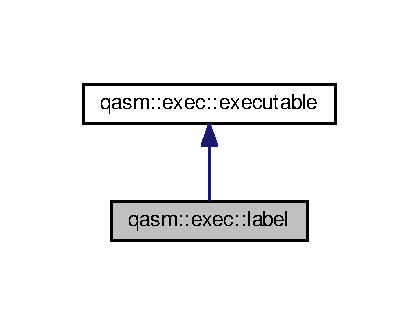
\includegraphics[width=201pt]{classqasm_1_1exec_1_1label__inherit__graph}
\end{center}
\end{figure}


Collaboration diagram for qasm\+:\+:exec\+:\+:label\+:
\nopagebreak
\begin{figure}[H]
\begin{center}
\leavevmode
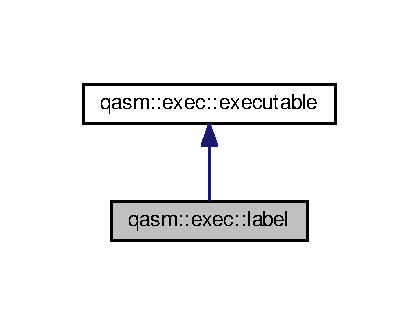
\includegraphics[width=201pt]{classqasm_1_1exec_1_1label__coll__graph}
\end{center}
\end{figure}
\subsection*{Public Member Functions}
\begin{DoxyCompactItemize}
\item 
\hyperlink{classqasm_1_1exec_1_1label_aea2a4500ead46240c26215b6d964fae4}{label} (string \hyperlink{classqasm_1_1exec_1_1label_ae88393dae0bd5ddbe32a65cfb2d8f247}{name})
\end{DoxyCompactItemize}
\subsection*{Public Attributes}
\begin{DoxyCompactItemize}
\item 
string \hyperlink{classqasm_1_1exec_1_1label_ae88393dae0bd5ddbe32a65cfb2d8f247}{name}
\end{DoxyCompactItemize}


\subsection{Detailed Description}
Instruction to label a line 

\subsection{Constructor \& Destructor Documentation}
\index{qasm\+::exec\+::label@{qasm\+::exec\+::label}!label@{label}}
\index{label@{label}!qasm\+::exec\+::label@{qasm\+::exec\+::label}}
\subsubsection[{\texorpdfstring{label(string name)}{label(string name)}}]{\setlength{\rightskip}{0pt plus 5cm}qasm\+::exec\+::label\+::label (
\begin{DoxyParamCaption}
\item[{string}]{name}
\end{DoxyParamCaption}
)\hspace{0.3cm}{\ttfamily [inline]}}\hypertarget{classqasm_1_1exec_1_1label_aea2a4500ead46240c26215b6d964fae4}{}\label{classqasm_1_1exec_1_1label_aea2a4500ead46240c26215b6d964fae4}


\subsection{Member Data Documentation}
\index{qasm\+::exec\+::label@{qasm\+::exec\+::label}!name@{name}}
\index{name@{name}!qasm\+::exec\+::label@{qasm\+::exec\+::label}}
\subsubsection[{\texorpdfstring{name}{name}}]{\setlength{\rightskip}{0pt plus 5cm}string qasm\+::exec\+::label\+::name}\hypertarget{classqasm_1_1exec_1_1label_ae88393dae0bd5ddbe32a65cfb2d8f247}{}\label{classqasm_1_1exec_1_1label_ae88393dae0bd5ddbe32a65cfb2d8f247}


The documentation for this class was generated from the following file\+:\begin{DoxyCompactItemize}
\item 
src/runtime/\hyperlink{runtime_8hpp}{runtime.\+hpp}\end{DoxyCompactItemize}

\hypertarget{classlexical_1_1lexeme}{}\section{lexical\+:\+:lexeme Class Reference}
\label{classlexical_1_1lexeme}\index{lexical\+::lexeme@{lexical\+::lexeme}}


{\ttfamily \#include $<$lexer.\+hpp$>$}

\subsection*{Public Member Functions}
\begin{DoxyCompactItemize}
\item 
\hyperlink{classlexical_1_1lexeme_a2a69e7860946ccb70ab8f8ca0970ca42}{lexeme} (std\+::string \hyperlink{classlexical_1_1lexeme_a43f46025bbc59bdaff06d4e4efc979c1}{name}, std\+::string \hyperlink{classlexical_1_1lexeme_a8265b6f1e87790a3ca3fcd82b5543726}{pattern})
\item 
bool \hyperlink{classlexical_1_1lexeme_a26fd45099f7e056db7f39cd9f222cf97}{matches} (std\+::string\+::iterator begin, std\+::string\+::iterator end)
\item 
\hyperlink{structlexical_1_1match}{match} \hyperlink{classlexical_1_1lexeme_ade092b47d889c338daa38902409747ab}{extract} (\hyperlink{types_8h_ab2bb0e5480d1d957383df6b350794313}{ulong} row, \hyperlink{types_8h_ab2bb0e5480d1d957383df6b350794313}{ulong} column, std\+::string\+::iterator begin, std\+::string\+::iterator end)
\end{DoxyCompactItemize}
\subsection*{Public Attributes}
\begin{DoxyCompactItemize}
\item 
std\+::string \hyperlink{classlexical_1_1lexeme_a43f46025bbc59bdaff06d4e4efc979c1}{name}
\item 
std\+::string \hyperlink{classlexical_1_1lexeme_a8265b6f1e87790a3ca3fcd82b5543726}{pattern}
\item 
std\+::regex \hyperlink{classlexical_1_1lexeme_a2185fc486b1c6c75a57a3e30155eed15}{rx}
\item 
bool \hyperlink{classlexical_1_1lexeme_accc3564ad951f163e3cf4dd8f93ede15}{skippable}
\end{DoxyCompactItemize}


\subsection{Detailed Description}
Class representing a lexical literal using regular expressions 

\subsection{Constructor \& Destructor Documentation}
\index{lexical\+::lexeme@{lexical\+::lexeme}!lexeme@{lexeme}}
\index{lexeme@{lexeme}!lexical\+::lexeme@{lexical\+::lexeme}}
\subsubsection[{\texorpdfstring{lexeme(std\+::string name, std\+::string pattern)}{lexeme(std::string name, std::string pattern)}}]{\setlength{\rightskip}{0pt plus 5cm}lexical\+::lexeme\+::lexeme (
\begin{DoxyParamCaption}
\item[{std\+::string}]{name, }
\item[{std\+::string}]{pattern}
\end{DoxyParamCaption}
)\hspace{0.3cm}{\ttfamily [inline]}}\hypertarget{classlexical_1_1lexeme_a2a69e7860946ccb70ab8f8ca0970ca42}{}\label{classlexical_1_1lexeme_a2a69e7860946ccb70ab8f8ca0970ca42}
Create a lexeme from a name and regex pattern 

\subsection{Member Function Documentation}
\index{lexical\+::lexeme@{lexical\+::lexeme}!extract@{extract}}
\index{extract@{extract}!lexical\+::lexeme@{lexical\+::lexeme}}
\subsubsection[{\texorpdfstring{extract(ulong row, ulong column, std\+::string\+::iterator begin, std\+::string\+::iterator end)}{extract(ulong row, ulong column, std::string::iterator begin, std::string::iterator end)}}]{\setlength{\rightskip}{0pt plus 5cm}{\bf match} lexical\+::lexeme\+::extract (
\begin{DoxyParamCaption}
\item[{{\bf ulong}}]{row, }
\item[{{\bf ulong}}]{column, }
\item[{std\+::string\+::iterator}]{begin, }
\item[{std\+::string\+::iterator}]{end}
\end{DoxyParamCaption}
)\hspace{0.3cm}{\ttfamily [inline]}}\hypertarget{classlexical_1_1lexeme_ade092b47d889c338daa38902409747ab}{}\label{classlexical_1_1lexeme_ade092b47d889c338daa38902409747ab}
Extract a match from a string \index{lexical\+::lexeme@{lexical\+::lexeme}!matches@{matches}}
\index{matches@{matches}!lexical\+::lexeme@{lexical\+::lexeme}}
\subsubsection[{\texorpdfstring{matches(std\+::string\+::iterator begin, std\+::string\+::iterator end)}{matches(std::string::iterator begin, std::string::iterator end)}}]{\setlength{\rightskip}{0pt plus 5cm}bool lexical\+::lexeme\+::matches (
\begin{DoxyParamCaption}
\item[{std\+::string\+::iterator}]{begin, }
\item[{std\+::string\+::iterator}]{end}
\end{DoxyParamCaption}
)\hspace{0.3cm}{\ttfamily [inline]}}\hypertarget{classlexical_1_1lexeme_a26fd45099f7e056db7f39cd9f222cf97}{}\label{classlexical_1_1lexeme_a26fd45099f7e056db7f39cd9f222cf97}
Test if this lexeme can be extracted from a string 

\subsection{Member Data Documentation}
\index{lexical\+::lexeme@{lexical\+::lexeme}!name@{name}}
\index{name@{name}!lexical\+::lexeme@{lexical\+::lexeme}}
\subsubsection[{\texorpdfstring{name}{name}}]{\setlength{\rightskip}{0pt plus 5cm}std\+::string lexical\+::lexeme\+::name}\hypertarget{classlexical_1_1lexeme_a43f46025bbc59bdaff06d4e4efc979c1}{}\label{classlexical_1_1lexeme_a43f46025bbc59bdaff06d4e4efc979c1}
Lexeme name \index{lexical\+::lexeme@{lexical\+::lexeme}!pattern@{pattern}}
\index{pattern@{pattern}!lexical\+::lexeme@{lexical\+::lexeme}}
\subsubsection[{\texorpdfstring{pattern}{pattern}}]{\setlength{\rightskip}{0pt plus 5cm}std\+::string lexical\+::lexeme\+::pattern}\hypertarget{classlexical_1_1lexeme_a8265b6f1e87790a3ca3fcd82b5543726}{}\label{classlexical_1_1lexeme_a8265b6f1e87790a3ca3fcd82b5543726}
Lexeme regular expression pattern \index{lexical\+::lexeme@{lexical\+::lexeme}!rx@{rx}}
\index{rx@{rx}!lexical\+::lexeme@{lexical\+::lexeme}}
\subsubsection[{\texorpdfstring{rx}{rx}}]{\setlength{\rightskip}{0pt plus 5cm}std\+::regex lexical\+::lexeme\+::rx}\hypertarget{classlexical_1_1lexeme_a2185fc486b1c6c75a57a3e30155eed15}{}\label{classlexical_1_1lexeme_a2185fc486b1c6c75a57a3e30155eed15}
Compiled regex lexeme \index{lexical\+::lexeme@{lexical\+::lexeme}!skippable@{skippable}}
\index{skippable@{skippable}!lexical\+::lexeme@{lexical\+::lexeme}}
\subsubsection[{\texorpdfstring{skippable}{skippable}}]{\setlength{\rightskip}{0pt plus 5cm}bool lexical\+::lexeme\+::skippable}\hypertarget{classlexical_1_1lexeme_accc3564ad951f163e3cf4dd8f93ede15}{}\label{classlexical_1_1lexeme_accc3564ad951f163e3cf4dd8f93ede15}
Flag to test if this lexeme can be skipped in results 

The documentation for this class was generated from the following file\+:\begin{DoxyCompactItemize}
\item 
src/runtime/\hyperlink{lexer_8hpp}{lexer.\+hpp}\end{DoxyCompactItemize}

\hypertarget{classlexical_1_1lexer}{}\section{lexical\+:\+:lexer Class Reference}
\label{classlexical_1_1lexer}\index{lexical\+::lexer@{lexical\+::lexer}}


{\ttfamily \#include $<$lexer.\+hpp$>$}

\subsection*{Public Member Functions}
\begin{DoxyCompactItemize}
\item 
\hyperlink{classlexical_1_1lexer_a5fb29e19937c0e78267c42e13cb545b6}{lexer} (std\+::vector$<$ \hyperlink{classlexical_1_1lexeme}{lexeme} $\ast$ $>$ \hyperlink{classlexical_1_1lexer_acf8db5ce39817336f4cf12294b09bfcc}{tokens})
\item 
std\+::vector$<$ \hyperlink{structlexical_1_1match}{match} $>$ \hyperlink{classlexical_1_1lexer_a89f9fd380037709ace9c8fe7604b5460}{tokenize} (std\+::string file, std\+::string\+::iterator begin, std\+::string\+::iterator end)
\end{DoxyCompactItemize}
\subsection*{Private Attributes}
\begin{DoxyCompactItemize}
\item 
std\+::vector$<$ \hyperlink{classlexical_1_1lexeme}{lexeme} $\ast$ $>$ \hyperlink{classlexical_1_1lexer_acf8db5ce39817336f4cf12294b09bfcc}{tokens}
\end{DoxyCompactItemize}


\subsection{Detailed Description}
Class to tokenzie input string 

\subsection{Constructor \& Destructor Documentation}
\index{lexical\+::lexer@{lexical\+::lexer}!lexer@{lexer}}
\index{lexer@{lexer}!lexical\+::lexer@{lexical\+::lexer}}
\subsubsection[{\texorpdfstring{lexer(std\+::vector$<$ lexeme $\ast$ $>$ tokens)}{lexer(std::vector< lexeme * > tokens)}}]{\setlength{\rightskip}{0pt plus 5cm}lexical\+::lexer\+::lexer (
\begin{DoxyParamCaption}
\item[{std\+::vector$<$ {\bf lexeme} $\ast$ $>$}]{tokens}
\end{DoxyParamCaption}
)\hspace{0.3cm}{\ttfamily [inline]}}\hypertarget{classlexical_1_1lexer_a5fb29e19937c0e78267c42e13cb545b6}{}\label{classlexical_1_1lexer_a5fb29e19937c0e78267c42e13cb545b6}
Create a new lexer from a list of lexemes 

\subsection{Member Function Documentation}
\index{lexical\+::lexer@{lexical\+::lexer}!tokenize@{tokenize}}
\index{tokenize@{tokenize}!lexical\+::lexer@{lexical\+::lexer}}
\subsubsection[{\texorpdfstring{tokenize(std\+::string file, std\+::string\+::iterator begin, std\+::string\+::iterator end)}{tokenize(std::string file, std::string::iterator begin, std::string::iterator end)}}]{\setlength{\rightskip}{0pt plus 5cm}std\+::vector$<${\bf match}$>$ lexical\+::lexer\+::tokenize (
\begin{DoxyParamCaption}
\item[{std\+::string}]{file, }
\item[{std\+::string\+::iterator}]{begin, }
\item[{std\+::string\+::iterator}]{end}
\end{DoxyParamCaption}
)\hspace{0.3cm}{\ttfamily [inline]}}\hypertarget{classlexical_1_1lexer_a89f9fd380037709ace9c8fe7604b5460}{}\label{classlexical_1_1lexer_a89f9fd380037709ace9c8fe7604b5460}
Tokenize an input string. Lexical exception will be thrown if an unrecognized symbol is reached 

\subsection{Member Data Documentation}
\index{lexical\+::lexer@{lexical\+::lexer}!tokens@{tokens}}
\index{tokens@{tokens}!lexical\+::lexer@{lexical\+::lexer}}
\subsubsection[{\texorpdfstring{tokens}{tokens}}]{\setlength{\rightskip}{0pt plus 5cm}std\+::vector$<${\bf lexeme}$\ast$$>$ lexical\+::lexer\+::tokens\hspace{0.3cm}{\ttfamily [private]}}\hypertarget{classlexical_1_1lexer_acf8db5ce39817336f4cf12294b09bfcc}{}\label{classlexical_1_1lexer_acf8db5ce39817336f4cf12294b09bfcc}
List of lexemes to extract 

The documentation for this class was generated from the following file\+:\begin{DoxyCompactItemize}
\item 
src/runtime/\hyperlink{lexer_8hpp}{lexer.\+hpp}\end{DoxyCompactItemize}

\hypertarget{classlexical_1_1lexicalexception}{}\section{lexical\+:\+:lexicalexception Class Reference}
\label{classlexical_1_1lexicalexception}\index{lexical\+::lexicalexception@{lexical\+::lexicalexception}}


{\ttfamily \#include $<$lexer.\+hpp$>$}



Inheritance diagram for lexical\+:\+:lexicalexception\+:\nopagebreak
\begin{figure}[H]
\begin{center}
\leavevmode
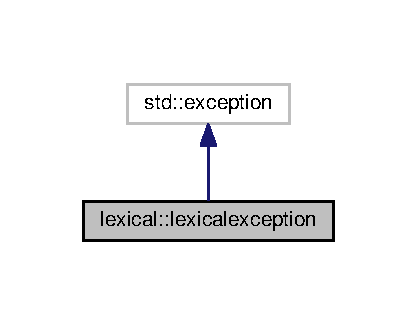
\includegraphics[width=200pt]{classlexical_1_1lexicalexception__inherit__graph}
\end{center}
\end{figure}


Collaboration diagram for lexical\+:\+:lexicalexception\+:\nopagebreak
\begin{figure}[H]
\begin{center}
\leavevmode
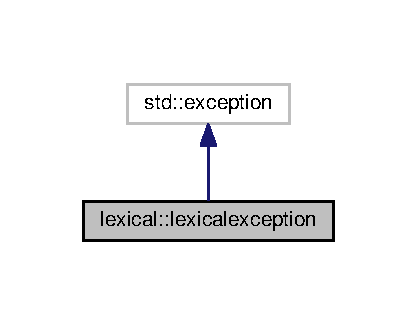
\includegraphics[width=200pt]{classlexical_1_1lexicalexception__coll__graph}
\end{center}
\end{figure}
\subsection*{Public Member Functions}
\begin{DoxyCompactItemize}
\item 
\hyperlink{classlexical_1_1lexicalexception_a669fdad5e3c9cfc1404b3cff07f2cc2c}{lexicalexception} (\hyperlink{types_8h_ab2bb0e5480d1d957383df6b350794313}{ulong} row, \hyperlink{types_8h_ab2bb0e5480d1d957383df6b350794313}{ulong} column, std\+::string \hyperlink{classlexical_1_1lexicalexception_a19c8e9b165ad5d2250d2a26c920462e3}{file}, std\+::string message)
\item 
const char $\ast$ \hyperlink{classlexical_1_1lexicalexception_a9d12fd196a80d2be20dfa616c063ffb4}{what} () const   throw ()
\end{DoxyCompactItemize}
\subsection*{Public Attributes}
\begin{DoxyCompactItemize}
\item 
\hyperlink{types_8h_ab2bb0e5480d1d957383df6b350794313}{ulong} \hyperlink{classlexical_1_1lexicalexception_a785417c9f8375670d73567db6562b74a}{r}
\item 
\hyperlink{types_8h_ab2bb0e5480d1d957383df6b350794313}{ulong} \hyperlink{classlexical_1_1lexicalexception_a7d7aeb97fa40e634950b28a3d48a9b51}{c}
\item 
std\+::string \hyperlink{classlexical_1_1lexicalexception_a19c8e9b165ad5d2250d2a26c920462e3}{file}
\item 
std\+::string \hyperlink{classlexical_1_1lexicalexception_aca4560509cfad8e43c42def571bba550}{msg}
\end{DoxyCompactItemize}
\subsection*{Private Attributes}
\begin{DoxyCompactItemize}
\item 
std\+::string \hyperlink{classlexical_1_1lexicalexception_ad116c229b30998b6630210dd86e8b10f}{what\+\_\+message}
\end{DoxyCompactItemize}


\subsection{Detailed Description}
Class representing an exception generated from the lexer 

\subsection{Constructor \& Destructor Documentation}
\index{lexical\+::lexicalexception@{lexical\+::lexicalexception}!lexicalexception@{lexicalexception}}
\index{lexicalexception@{lexicalexception}!lexical\+::lexicalexception@{lexical\+::lexicalexception}}
\subsubsection[{\texorpdfstring{lexicalexception(ulong row, ulong column, std\+::string file, std\+::string message)}{lexicalexception(ulong row, ulong column, std::string file, std::string message)}}]{\setlength{\rightskip}{0pt plus 5cm}lexical\+::lexicalexception\+::lexicalexception (
\begin{DoxyParamCaption}
\item[{{\bf ulong}}]{row, }
\item[{{\bf ulong}}]{column, }
\item[{std\+::string}]{file, }
\item[{std\+::string}]{message}
\end{DoxyParamCaption}
)\hspace{0.3cm}{\ttfamily [inline]}}\hypertarget{classlexical_1_1lexicalexception_a669fdad5e3c9cfc1404b3cff07f2cc2c}{}\label{classlexical_1_1lexicalexception_a669fdad5e3c9cfc1404b3cff07f2cc2c}
Create a new exception 

\subsection{Member Function Documentation}
\index{lexical\+::lexicalexception@{lexical\+::lexicalexception}!what@{what}}
\index{what@{what}!lexical\+::lexicalexception@{lexical\+::lexicalexception}}
\subsubsection[{\texorpdfstring{what() const }{what() const }}]{\setlength{\rightskip}{0pt plus 5cm}const char$\ast$ lexical\+::lexicalexception\+::what (
\begin{DoxyParamCaption}
{}
\end{DoxyParamCaption}
) const throw  ) \hspace{0.3cm}{\ttfamily [inline]}}\hypertarget{classlexical_1_1lexicalexception_a9d12fd196a80d2be20dfa616c063ffb4}{}\label{classlexical_1_1lexicalexception_a9d12fd196a80d2be20dfa616c063ffb4}
Print the message 

\subsection{Member Data Documentation}
\index{lexical\+::lexicalexception@{lexical\+::lexicalexception}!c@{c}}
\index{c@{c}!lexical\+::lexicalexception@{lexical\+::lexicalexception}}
\subsubsection[{\texorpdfstring{c}{c}}]{\setlength{\rightskip}{0pt plus 5cm}{\bf ulong} lexical\+::lexicalexception\+::c}\hypertarget{classlexical_1_1lexicalexception_a7d7aeb97fa40e634950b28a3d48a9b51}{}\label{classlexical_1_1lexicalexception_a7d7aeb97fa40e634950b28a3d48a9b51}
Column exception occurred on \index{lexical\+::lexicalexception@{lexical\+::lexicalexception}!file@{file}}
\index{file@{file}!lexical\+::lexicalexception@{lexical\+::lexicalexception}}
\subsubsection[{\texorpdfstring{file}{file}}]{\setlength{\rightskip}{0pt plus 5cm}std\+::string lexical\+::lexicalexception\+::file}\hypertarget{classlexical_1_1lexicalexception_a19c8e9b165ad5d2250d2a26c920462e3}{}\label{classlexical_1_1lexicalexception_a19c8e9b165ad5d2250d2a26c920462e3}
File name exception occurred in \index{lexical\+::lexicalexception@{lexical\+::lexicalexception}!msg@{msg}}
\index{msg@{msg}!lexical\+::lexicalexception@{lexical\+::lexicalexception}}
\subsubsection[{\texorpdfstring{msg}{msg}}]{\setlength{\rightskip}{0pt plus 5cm}std\+::string lexical\+::lexicalexception\+::msg}\hypertarget{classlexical_1_1lexicalexception_aca4560509cfad8e43c42def571bba550}{}\label{classlexical_1_1lexicalexception_aca4560509cfad8e43c42def571bba550}
Message for this exception \index{lexical\+::lexicalexception@{lexical\+::lexicalexception}!r@{r}}
\index{r@{r}!lexical\+::lexicalexception@{lexical\+::lexicalexception}}
\subsubsection[{\texorpdfstring{r}{r}}]{\setlength{\rightskip}{0pt plus 5cm}{\bf ulong} lexical\+::lexicalexception\+::r}\hypertarget{classlexical_1_1lexicalexception_a785417c9f8375670d73567db6562b74a}{}\label{classlexical_1_1lexicalexception_a785417c9f8375670d73567db6562b74a}
Row exception occurred on \index{lexical\+::lexicalexception@{lexical\+::lexicalexception}!what\+\_\+message@{what\+\_\+message}}
\index{what\+\_\+message@{what\+\_\+message}!lexical\+::lexicalexception@{lexical\+::lexicalexception}}
\subsubsection[{\texorpdfstring{what\+\_\+message}{what_message}}]{\setlength{\rightskip}{0pt plus 5cm}std\+::string lexical\+::lexicalexception\+::what\+\_\+message\hspace{0.3cm}{\ttfamily [private]}}\hypertarget{classlexical_1_1lexicalexception_ad116c229b30998b6630210dd86e8b10f}{}\label{classlexical_1_1lexicalexception_ad116c229b30998b6630210dd86e8b10f}
Combined exception message 

The documentation for this class was generated from the following file\+:\begin{DoxyCompactItemize}
\item 
src/runtime/\hyperlink{lexer_8hpp}{lexer.\+hpp}\end{DoxyCompactItemize}

\hypertarget{classresources_1_1Loader}{}\section{resources.\+Loader Class Reference}
\label{classresources_1_1Loader}\index{resources.\+Loader@{resources.\+Loader}}


Collaboration diagram for resources.\+Loader\+:\nopagebreak
\begin{figure}[H]
\begin{center}
\leavevmode
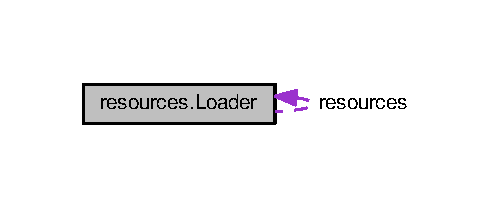
\includegraphics[width=236pt]{classresources_1_1Loader__coll__graph}
\end{center}
\end{figure}
\subsection*{Public Member Functions}
\begin{DoxyCompactItemize}
\item 
Image \hyperlink{classresources_1_1Loader_ab70c0099b53e57b6ce64132291e4f29d}{load} (String resource)  throws I\+O\+Exception 
\end{DoxyCompactItemize}
\subsection*{Static Public Attributes}
\begin{DoxyCompactItemize}
\item 
static \hyperlink{classresources_1_1Loader}{Loader} \hyperlink{classresources_1_1Loader_a007cafedd048831f9d18ba4b8ac768ff}{resources} = new \hyperlink{classresources_1_1Loader}{Loader}()
\end{DoxyCompactItemize}


\subsection{Detailed Description}
\begin{DoxyAuthor}{Author}
halse 
\end{DoxyAuthor}


\subsection{Member Function Documentation}
\index{resources\+::\+Loader@{resources\+::\+Loader}!load@{load}}
\index{load@{load}!resources\+::\+Loader@{resources\+::\+Loader}}
\subsubsection[{\texorpdfstring{load(\+String resource)}{load(String resource)}}]{\setlength{\rightskip}{0pt plus 5cm}Image resources.\+Loader.\+load (
\begin{DoxyParamCaption}
\item[{String}]{resource}
\end{DoxyParamCaption}
) throws I\+O\+Exception\hspace{0.3cm}{\ttfamily [inline]}}\hypertarget{classresources_1_1Loader_ab70c0099b53e57b6ce64132291e4f29d}{}\label{classresources_1_1Loader_ab70c0099b53e57b6ce64132291e4f29d}


\subsection{Member Data Documentation}
\index{resources\+::\+Loader@{resources\+::\+Loader}!resources@{resources}}
\index{resources@{resources}!resources\+::\+Loader@{resources\+::\+Loader}}
\subsubsection[{\texorpdfstring{resources}{resources}}]{\setlength{\rightskip}{0pt plus 5cm}{\bf Loader} resources.\+Loader.\+resources = new {\bf Loader}()\hspace{0.3cm}{\ttfamily [static]}}\hypertarget{classresources_1_1Loader_a007cafedd048831f9d18ba4b8ac768ff}{}\label{classresources_1_1Loader_a007cafedd048831f9d18ba4b8ac768ff}


The documentation for this class was generated from the following file\+:\begin{DoxyCompactItemize}
\item 
src/ide/src/resources/\hyperlink{Loader_8java}{Loader.\+java}\end{DoxyCompactItemize}

\hypertarget{structlexical_1_1match}{}\section{lexical\+:\+:match Struct Reference}
\label{structlexical_1_1match}\index{lexical\+::match@{lexical\+::match}}


{\ttfamily \#include $<$lexer.\+hpp$>$}



Collaboration diagram for lexical\+:\+:match\+:\nopagebreak
\begin{figure}[H]
\begin{center}
\leavevmode
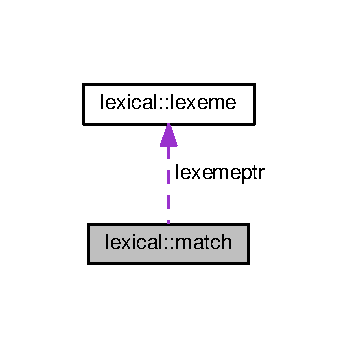
\includegraphics[width=167pt]{structlexical_1_1match__coll__graph}
\end{center}
\end{figure}
\subsection*{Public Member Functions}
\begin{DoxyCompactItemize}
\item 
\hyperlink{structlexical_1_1match_ace4aee5410296a2cfca192700098891a}{match} ()
\item 
std\+::string \hyperlink{structlexical_1_1match_a09ae2bd81b43191fa58ce13c2245b6f9}{to\+String} ()
\item 
bool \hyperlink{structlexical_1_1match_aafa3ddcad89ea3abb86b557cafe3e0d7}{match\+Exists} ()
\end{DoxyCompactItemize}
\subsection*{Public Attributes}
\begin{DoxyCompactItemize}
\item 
\hyperlink{classlexical_1_1lexeme}{lexeme} $\ast$ \hyperlink{structlexical_1_1match_a346ef13017b47ee41a6abe643e5732e1}{lexemeptr}
\item 
std\+::match\+\_\+results$<$ std\+::string\+::iterator $>$ \hyperlink{structlexical_1_1match_a2ebda7888d347b3de302ffc465755f07}{content}
\item 
\hyperlink{types_8h_ab2bb0e5480d1d957383df6b350794313}{ulong} \hyperlink{structlexical_1_1match_a854a8828680bbfc08aa214e875ba5514}{row\+\_\+start}
\item 
\hyperlink{types_8h_ab2bb0e5480d1d957383df6b350794313}{ulong} \hyperlink{structlexical_1_1match_a3a1754ba678051a508ee2889c4a5f4eb}{column\+\_\+start}
\item 
\hyperlink{types_8h_ab2bb0e5480d1d957383df6b350794313}{ulong} \hyperlink{structlexical_1_1match_abf7eca2de9cee016df02265a38666486}{row\+\_\+end}
\item 
\hyperlink{types_8h_ab2bb0e5480d1d957383df6b350794313}{ulong} \hyperlink{structlexical_1_1match_ac9b0f6134b653452a2b0ff8b36c89729}{column\+\_\+end}
\end{DoxyCompactItemize}


\subsection{Detailed Description}
Class representing a regex match in a lexed document including row and column indexes 

\subsection{Constructor \& Destructor Documentation}
\index{lexical\+::match@{lexical\+::match}!match@{match}}
\index{match@{match}!lexical\+::match@{lexical\+::match}}
\subsubsection[{\texorpdfstring{match()}{match()}}]{\setlength{\rightskip}{0pt plus 5cm}lexical\+::match\+::match (
\begin{DoxyParamCaption}
{}
\end{DoxyParamCaption}
)\hspace{0.3cm}{\ttfamily [inline]}}\hypertarget{structlexical_1_1match_ace4aee5410296a2cfca192700098891a}{}\label{structlexical_1_1match_ace4aee5410296a2cfca192700098891a}
Match constructor 

\subsection{Member Function Documentation}
\index{lexical\+::match@{lexical\+::match}!match\+Exists@{match\+Exists}}
\index{match\+Exists@{match\+Exists}!lexical\+::match@{lexical\+::match}}
\subsubsection[{\texorpdfstring{match\+Exists()}{matchExists()}}]{\setlength{\rightskip}{0pt plus 5cm}bool lexical\+::match\+::match\+Exists (
\begin{DoxyParamCaption}
{}
\end{DoxyParamCaption}
)\hspace{0.3cm}{\ttfamily [inline]}}\hypertarget{structlexical_1_1match_aafa3ddcad89ea3abb86b557cafe3e0d7}{}\label{structlexical_1_1match_aafa3ddcad89ea3abb86b557cafe3e0d7}
Test if this match is valid \index{lexical\+::match@{lexical\+::match}!to\+String@{to\+String}}
\index{to\+String@{to\+String}!lexical\+::match@{lexical\+::match}}
\subsubsection[{\texorpdfstring{to\+String()}{toString()}}]{\setlength{\rightskip}{0pt plus 5cm}std\+::string lexical\+::match\+::to\+String (
\begin{DoxyParamCaption}
{}
\end{DoxyParamCaption}
)\hspace{0.3cm}{\ttfamily [inline]}}\hypertarget{structlexical_1_1match_a09ae2bd81b43191fa58ce13c2245b6f9}{}\label{structlexical_1_1match_a09ae2bd81b43191fa58ce13c2245b6f9}
Print match to string 

\subsection{Member Data Documentation}
\index{lexical\+::match@{lexical\+::match}!column\+\_\+end@{column\+\_\+end}}
\index{column\+\_\+end@{column\+\_\+end}!lexical\+::match@{lexical\+::match}}
\subsubsection[{\texorpdfstring{column\+\_\+end}{column_end}}]{\setlength{\rightskip}{0pt plus 5cm}{\bf ulong} lexical\+::match\+::column\+\_\+end}\hypertarget{structlexical_1_1match_ac9b0f6134b653452a2b0ff8b36c89729}{}\label{structlexical_1_1match_ac9b0f6134b653452a2b0ff8b36c89729}
End column of match in source file \index{lexical\+::match@{lexical\+::match}!column\+\_\+start@{column\+\_\+start}}
\index{column\+\_\+start@{column\+\_\+start}!lexical\+::match@{lexical\+::match}}
\subsubsection[{\texorpdfstring{column\+\_\+start}{column_start}}]{\setlength{\rightskip}{0pt plus 5cm}{\bf ulong} lexical\+::match\+::column\+\_\+start}\hypertarget{structlexical_1_1match_a3a1754ba678051a508ee2889c4a5f4eb}{}\label{structlexical_1_1match_a3a1754ba678051a508ee2889c4a5f4eb}
Start column of match in source file \index{lexical\+::match@{lexical\+::match}!content@{content}}
\index{content@{content}!lexical\+::match@{lexical\+::match}}
\subsubsection[{\texorpdfstring{content}{content}}]{\setlength{\rightskip}{0pt plus 5cm}std\+::match\+\_\+results$<$std\+::string\+::iterator$>$ lexical\+::match\+::content}\hypertarget{structlexical_1_1match_a2ebda7888d347b3de302ffc465755f07}{}\label{structlexical_1_1match_a2ebda7888d347b3de302ffc465755f07}
Regular expression match contents \index{lexical\+::match@{lexical\+::match}!lexemeptr@{lexemeptr}}
\index{lexemeptr@{lexemeptr}!lexical\+::match@{lexical\+::match}}
\subsubsection[{\texorpdfstring{lexemeptr}{lexemeptr}}]{\setlength{\rightskip}{0pt plus 5cm}{\bf lexeme}$\ast$ lexical\+::match\+::lexemeptr}\hypertarget{structlexical_1_1match_a346ef13017b47ee41a6abe643e5732e1}{}\label{structlexical_1_1match_a346ef13017b47ee41a6abe643e5732e1}
Pointer to the associated lexeme this match was extracted from \index{lexical\+::match@{lexical\+::match}!row\+\_\+end@{row\+\_\+end}}
\index{row\+\_\+end@{row\+\_\+end}!lexical\+::match@{lexical\+::match}}
\subsubsection[{\texorpdfstring{row\+\_\+end}{row_end}}]{\setlength{\rightskip}{0pt plus 5cm}{\bf ulong} lexical\+::match\+::row\+\_\+end}\hypertarget{structlexical_1_1match_abf7eca2de9cee016df02265a38666486}{}\label{structlexical_1_1match_abf7eca2de9cee016df02265a38666486}
End row of match in source file \index{lexical\+::match@{lexical\+::match}!row\+\_\+start@{row\+\_\+start}}
\index{row\+\_\+start@{row\+\_\+start}!lexical\+::match@{lexical\+::match}}
\subsubsection[{\texorpdfstring{row\+\_\+start}{row_start}}]{\setlength{\rightskip}{0pt plus 5cm}{\bf ulong} lexical\+::match\+::row\+\_\+start}\hypertarget{structlexical_1_1match_a854a8828680bbfc08aa214e875ba5514}{}\label{structlexical_1_1match_a854a8828680bbfc08aa214e875ba5514}
Start row of match in source file 

The documentation for this struct was generated from the following file\+:\begin{DoxyCompactItemize}
\item 
src/runtime/\hyperlink{lexer_8hpp}{lexer.\+hpp}\end{DoxyCompactItemize}

\hypertarget{classqlib_1_1math_1_1matrix}{}\section{qlib\+:\+:math\+:\+:matrix Class Reference}
\label{classqlib_1_1math_1_1matrix}\index{qlib\+::math\+::matrix@{qlib\+::math\+::matrix}}


{\ttfamily \#include $<$matrix.\+hpp$>$}



Inheritance diagram for qlib\+:\+:math\+:\+:matrix\+:\nopagebreak
\begin{figure}[H]
\begin{center}
\leavevmode
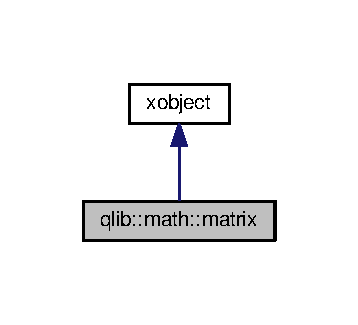
\includegraphics[width=172pt]{classqlib_1_1math_1_1matrix__inherit__graph}
\end{center}
\end{figure}


Collaboration diagram for qlib\+:\+:math\+:\+:matrix\+:\nopagebreak
\begin{figure}[H]
\begin{center}
\leavevmode
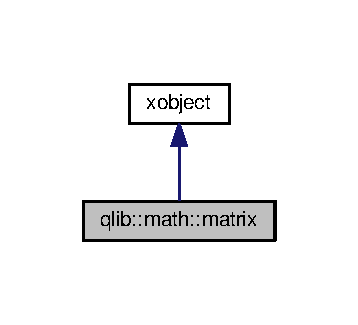
\includegraphics[width=172pt]{classqlib_1_1math_1_1matrix__coll__graph}
\end{center}
\end{figure}
\subsection*{Public Member Functions}
\begin{DoxyCompactItemize}
\item 
\hyperlink{classqlib_1_1math_1_1matrix_a6e66a3f67ecf06a42068d2dbf8885e66}{matrix} (size\+\_\+t \hyperlink{classqlib_1_1math_1_1matrix_af29b6ea4316eb972bbdc55da6e54dbb3}{rows}, size\+\_\+t \hyperlink{classqlib_1_1math_1_1matrix_ad3c2dd80c600d7bf37ae5bbdf5f056b8}{columns})
\item 
\hyperlink{classqlib_1_1math_1_1matrix_a8cbac1f2ae9917a4742cd0d147e3ba9b}{matrix} (size\+\_\+t \hyperlink{classqlib_1_1math_1_1matrix_af29b6ea4316eb972bbdc55da6e54dbb3}{rows}, size\+\_\+t \hyperlink{classqlib_1_1math_1_1matrix_ad3c2dd80c600d7bf37ae5bbdf5f056b8}{columns}, std\+::vector$<$ \hyperlink{classqlib_1_1math_1_1complex}{complex} $>$ \hyperlink{classqlib_1_1math_1_1matrix_ad764d65375ba1e50381f640bdc181c0b}{values})
\item 
\hyperlink{classqlib_1_1math_1_1matrix_afebdd1cf189728ace53a594d5ef8b750}{$\sim$matrix} ()
\item 
\hyperlink{classqlib_1_1math_1_1complex}{complex} \& \hyperlink{classqlib_1_1math_1_1matrix_a50cbbef6e5b7888aecffbf66def70154}{operator()} (size\+\_\+t r, size\+\_\+t c)
\item 
\hyperlink{classqlib_1_1math_1_1complex}{complex} \& \hyperlink{classqlib_1_1math_1_1matrix_af93c414d328b985c83c032f41f485a9a}{operator()} (size\+\_\+t idx)
\item 
size\+\_\+t \hyperlink{classqlib_1_1math_1_1matrix_add844c31055d495274b037e7bcd8f0b7}{count\+Rows} ()
\item 
size\+\_\+t \hyperlink{classqlib_1_1math_1_1matrix_a69ed708edf603637731e4f6fe46b0754}{count\+Columns} ()
\item 
size\+\_\+t \hyperlink{classqlib_1_1math_1_1matrix_a2f0ada8003cf2306534700502f598428}{size} ()
\item 
void \hyperlink{classqlib_1_1math_1_1matrix_a2d09bd42691acdbf315d5cbd7a698698}{set} (size\+\_\+t r, size\+\_\+t c, \hyperlink{classqlib_1_1math_1_1complex}{complex} value)
\item 
void \hyperlink{classqlib_1_1math_1_1matrix_ae97863a30bb445897ff63c77582a366a}{set} (size\+\_\+t idx, \hyperlink{classqlib_1_1math_1_1complex}{complex} value)
\item 
\hyperlink{classqlib_1_1math_1_1complex}{complex} \hyperlink{classqlib_1_1math_1_1matrix_a91fcadaccfcd68adb71de0da6f5d267f}{get} (size\+\_\+t r, size\+\_\+t c)
\item 
\hyperlink{classqlib_1_1math_1_1complex}{complex} \hyperlink{classqlib_1_1math_1_1matrix_a17dce2bfd8addcb026f6d9159134f1c7}{get} (size\+\_\+t idx)
\item 
std\+::string \hyperlink{classqlib_1_1math_1_1matrix_a06ec639a654b5319f4eb1bff591d6e7b}{to\+String} ()
\item 
std\+::vector$<$ \hyperlink{classqlib_1_1math_1_1complex}{complex} $>$\+::iterator \hyperlink{classqlib_1_1math_1_1matrix_a1cbe9185c4f147d821eeb0b36ed9cc86}{begin} ()
\item 
std\+::vector$<$ \hyperlink{classqlib_1_1math_1_1complex}{complex} $>$\+::iterator \hyperlink{classqlib_1_1math_1_1matrix_ae250bb5455fe71b836a5252335575545}{end} ()
\end{DoxyCompactItemize}
\subsection*{Private Attributes}
\begin{DoxyCompactItemize}
\item 
std\+::vector$<$ \hyperlink{classqlib_1_1math_1_1complex}{complex} $>$ \hyperlink{classqlib_1_1math_1_1matrix_ad764d65375ba1e50381f640bdc181c0b}{values}
\item 
size\+\_\+t \hyperlink{classqlib_1_1math_1_1matrix_af29b6ea4316eb972bbdc55da6e54dbb3}{rows}
\item 
size\+\_\+t \hyperlink{classqlib_1_1math_1_1matrix_ad3c2dd80c600d7bf37ae5bbdf5f056b8}{columns}
\item 
size\+\_\+t \hyperlink{classqlib_1_1math_1_1matrix_aef00292f85054708922acef6b7744a40}{length}
\end{DoxyCompactItemize}


\subsection{Detailed Description}
Complex matrix class 

\subsection{Constructor \& Destructor Documentation}
\index{qlib\+::math\+::matrix@{qlib\+::math\+::matrix}!matrix@{matrix}}
\index{matrix@{matrix}!qlib\+::math\+::matrix@{qlib\+::math\+::matrix}}
\subsubsection[{\texorpdfstring{matrix(size\+\_\+t rows, size\+\_\+t columns)}{matrix(size_t rows, size_t columns)}}]{\setlength{\rightskip}{0pt plus 5cm}qlib\+::math\+::matrix\+::matrix (
\begin{DoxyParamCaption}
\item[{size\+\_\+t}]{rows, }
\item[{size\+\_\+t}]{columns}
\end{DoxyParamCaption}
)\hspace{0.3cm}{\ttfamily [inline]}}\hypertarget{classqlib_1_1math_1_1matrix_a6e66a3f67ecf06a42068d2dbf8885e66}{}\label{classqlib_1_1math_1_1matrix_a6e66a3f67ecf06a42068d2dbf8885e66}
Create an empty matrix of this size \index{qlib\+::math\+::matrix@{qlib\+::math\+::matrix}!matrix@{matrix}}
\index{matrix@{matrix}!qlib\+::math\+::matrix@{qlib\+::math\+::matrix}}
\subsubsection[{\texorpdfstring{matrix(size\+\_\+t rows, size\+\_\+t columns, std\+::vector$<$ complex $>$ values)}{matrix(size_t rows, size_t columns, std::vector< complex > values)}}]{\setlength{\rightskip}{0pt plus 5cm}qlib\+::math\+::matrix\+::matrix (
\begin{DoxyParamCaption}
\item[{size\+\_\+t}]{rows, }
\item[{size\+\_\+t}]{columns, }
\item[{std\+::vector$<$ {\bf complex} $>$}]{values}
\end{DoxyParamCaption}
)\hspace{0.3cm}{\ttfamily [inline]}}\hypertarget{classqlib_1_1math_1_1matrix_a8cbac1f2ae9917a4742cd0d147e3ba9b}{}\label{classqlib_1_1math_1_1matrix_a8cbac1f2ae9917a4742cd0d147e3ba9b}
Create a matrix of this size with the given values in compressed row-\/$>$column form \index{qlib\+::math\+::matrix@{qlib\+::math\+::matrix}!````~matrix@{$\sim$matrix}}
\index{````~matrix@{$\sim$matrix}!qlib\+::math\+::matrix@{qlib\+::math\+::matrix}}
\subsubsection[{\texorpdfstring{$\sim$matrix()}{~matrix()}}]{\setlength{\rightskip}{0pt plus 5cm}qlib\+::math\+::matrix\+::$\sim$matrix (
\begin{DoxyParamCaption}
{}
\end{DoxyParamCaption}
)\hspace{0.3cm}{\ttfamily [inline]}}\hypertarget{classqlib_1_1math_1_1matrix_afebdd1cf189728ace53a594d5ef8b750}{}\label{classqlib_1_1math_1_1matrix_afebdd1cf189728ace53a594d5ef8b750}
Matrix destructor 

\subsection{Member Function Documentation}
\index{qlib\+::math\+::matrix@{qlib\+::math\+::matrix}!begin@{begin}}
\index{begin@{begin}!qlib\+::math\+::matrix@{qlib\+::math\+::matrix}}
\subsubsection[{\texorpdfstring{begin()}{begin()}}]{\setlength{\rightskip}{0pt plus 5cm}std\+::vector$<${\bf complex}$>$\+::iterator qlib\+::math\+::matrix\+::begin (
\begin{DoxyParamCaption}
{}
\end{DoxyParamCaption}
)\hspace{0.3cm}{\ttfamily [inline]}}\hypertarget{classqlib_1_1math_1_1matrix_a1cbe9185c4f147d821eeb0b36ed9cc86}{}\label{classqlib_1_1math_1_1matrix_a1cbe9185c4f147d821eeb0b36ed9cc86}
Iterator starting at element 0,0 \index{qlib\+::math\+::matrix@{qlib\+::math\+::matrix}!count\+Columns@{count\+Columns}}
\index{count\+Columns@{count\+Columns}!qlib\+::math\+::matrix@{qlib\+::math\+::matrix}}
\subsubsection[{\texorpdfstring{count\+Columns()}{countColumns()}}]{\setlength{\rightskip}{0pt plus 5cm}size\+\_\+t qlib\+::math\+::matrix\+::count\+Columns (
\begin{DoxyParamCaption}
{}
\end{DoxyParamCaption}
)\hspace{0.3cm}{\ttfamily [inline]}}\hypertarget{classqlib_1_1math_1_1matrix_a69ed708edf603637731e4f6fe46b0754}{}\label{classqlib_1_1math_1_1matrix_a69ed708edf603637731e4f6fe46b0754}
Number of columns \index{qlib\+::math\+::matrix@{qlib\+::math\+::matrix}!count\+Rows@{count\+Rows}}
\index{count\+Rows@{count\+Rows}!qlib\+::math\+::matrix@{qlib\+::math\+::matrix}}
\subsubsection[{\texorpdfstring{count\+Rows()}{countRows()}}]{\setlength{\rightskip}{0pt plus 5cm}size\+\_\+t qlib\+::math\+::matrix\+::count\+Rows (
\begin{DoxyParamCaption}
{}
\end{DoxyParamCaption}
)\hspace{0.3cm}{\ttfamily [inline]}}\hypertarget{classqlib_1_1math_1_1matrix_add844c31055d495274b037e7bcd8f0b7}{}\label{classqlib_1_1math_1_1matrix_add844c31055d495274b037e7bcd8f0b7}
Number of rows \index{qlib\+::math\+::matrix@{qlib\+::math\+::matrix}!end@{end}}
\index{end@{end}!qlib\+::math\+::matrix@{qlib\+::math\+::matrix}}
\subsubsection[{\texorpdfstring{end()}{end()}}]{\setlength{\rightskip}{0pt plus 5cm}std\+::vector$<${\bf complex}$>$\+::iterator qlib\+::math\+::matrix\+::end (
\begin{DoxyParamCaption}
{}
\end{DoxyParamCaption}
)\hspace{0.3cm}{\ttfamily [inline]}}\hypertarget{classqlib_1_1math_1_1matrix_ae250bb5455fe71b836a5252335575545}{}\label{classqlib_1_1math_1_1matrix_ae250bb5455fe71b836a5252335575545}
Iterator starting after element rows-\/1,columns-\/1 \index{qlib\+::math\+::matrix@{qlib\+::math\+::matrix}!get@{get}}
\index{get@{get}!qlib\+::math\+::matrix@{qlib\+::math\+::matrix}}
\subsubsection[{\texorpdfstring{get(size\+\_\+t r, size\+\_\+t c)}{get(size_t r, size_t c)}}]{\setlength{\rightskip}{0pt plus 5cm}{\bf complex} qlib\+::math\+::matrix\+::get (
\begin{DoxyParamCaption}
\item[{size\+\_\+t}]{r, }
\item[{size\+\_\+t}]{c}
\end{DoxyParamCaption}
)\hspace{0.3cm}{\ttfamily [inline]}}\hypertarget{classqlib_1_1math_1_1matrix_a91fcadaccfcd68adb71de0da6f5d267f}{}\label{classqlib_1_1math_1_1matrix_a91fcadaccfcd68adb71de0da6f5d267f}
Get element from matrix \index{qlib\+::math\+::matrix@{qlib\+::math\+::matrix}!get@{get}}
\index{get@{get}!qlib\+::math\+::matrix@{qlib\+::math\+::matrix}}
\subsubsection[{\texorpdfstring{get(size\+\_\+t idx)}{get(size_t idx)}}]{\setlength{\rightskip}{0pt plus 5cm}{\bf complex} qlib\+::math\+::matrix\+::get (
\begin{DoxyParamCaption}
\item[{size\+\_\+t}]{idx}
\end{DoxyParamCaption}
)\hspace{0.3cm}{\ttfamily [inline]}}\hypertarget{classqlib_1_1math_1_1matrix_a17dce2bfd8addcb026f6d9159134f1c7}{}\label{classqlib_1_1math_1_1matrix_a17dce2bfd8addcb026f6d9159134f1c7}
Get element from matrix \index{qlib\+::math\+::matrix@{qlib\+::math\+::matrix}!operator()@{operator()}}
\index{operator()@{operator()}!qlib\+::math\+::matrix@{qlib\+::math\+::matrix}}
\subsubsection[{\texorpdfstring{operator()(size\+\_\+t r, size\+\_\+t c)}{operator()(size_t r, size_t c)}}]{\setlength{\rightskip}{0pt plus 5cm}{\bf complex}\& qlib\+::math\+::matrix\+::operator() (
\begin{DoxyParamCaption}
\item[{size\+\_\+t}]{r, }
\item[{size\+\_\+t}]{c}
\end{DoxyParamCaption}
)\hspace{0.3cm}{\ttfamily [inline]}}\hypertarget{classqlib_1_1math_1_1matrix_a50cbbef6e5b7888aecffbf66def70154}{}\label{classqlib_1_1math_1_1matrix_a50cbbef6e5b7888aecffbf66def70154}
Get element from matrix \index{qlib\+::math\+::matrix@{qlib\+::math\+::matrix}!operator()@{operator()}}
\index{operator()@{operator()}!qlib\+::math\+::matrix@{qlib\+::math\+::matrix}}
\subsubsection[{\texorpdfstring{operator()(size\+\_\+t idx)}{operator()(size_t idx)}}]{\setlength{\rightskip}{0pt plus 5cm}{\bf complex}\& qlib\+::math\+::matrix\+::operator() (
\begin{DoxyParamCaption}
\item[{size\+\_\+t}]{idx}
\end{DoxyParamCaption}
)\hspace{0.3cm}{\ttfamily [inline]}}\hypertarget{classqlib_1_1math_1_1matrix_af93c414d328b985c83c032f41f485a9a}{}\label{classqlib_1_1math_1_1matrix_af93c414d328b985c83c032f41f485a9a}
Get element from matrix \index{qlib\+::math\+::matrix@{qlib\+::math\+::matrix}!set@{set}}
\index{set@{set}!qlib\+::math\+::matrix@{qlib\+::math\+::matrix}}
\subsubsection[{\texorpdfstring{set(size\+\_\+t r, size\+\_\+t c, complex value)}{set(size_t r, size_t c, complex value)}}]{\setlength{\rightskip}{0pt plus 5cm}void qlib\+::math\+::matrix\+::set (
\begin{DoxyParamCaption}
\item[{size\+\_\+t}]{r, }
\item[{size\+\_\+t}]{c, }
\item[{{\bf complex}}]{value}
\end{DoxyParamCaption}
)\hspace{0.3cm}{\ttfamily [inline]}}\hypertarget{classqlib_1_1math_1_1matrix_a2d09bd42691acdbf315d5cbd7a698698}{}\label{classqlib_1_1math_1_1matrix_a2d09bd42691acdbf315d5cbd7a698698}
Set element in matrix \index{qlib\+::math\+::matrix@{qlib\+::math\+::matrix}!set@{set}}
\index{set@{set}!qlib\+::math\+::matrix@{qlib\+::math\+::matrix}}
\subsubsection[{\texorpdfstring{set(size\+\_\+t idx, complex value)}{set(size_t idx, complex value)}}]{\setlength{\rightskip}{0pt plus 5cm}void qlib\+::math\+::matrix\+::set (
\begin{DoxyParamCaption}
\item[{size\+\_\+t}]{idx, }
\item[{{\bf complex}}]{value}
\end{DoxyParamCaption}
)\hspace{0.3cm}{\ttfamily [inline]}}\hypertarget{classqlib_1_1math_1_1matrix_ae97863a30bb445897ff63c77582a366a}{}\label{classqlib_1_1math_1_1matrix_ae97863a30bb445897ff63c77582a366a}
Set element in matrix \index{qlib\+::math\+::matrix@{qlib\+::math\+::matrix}!size@{size}}
\index{size@{size}!qlib\+::math\+::matrix@{qlib\+::math\+::matrix}}
\subsubsection[{\texorpdfstring{size()}{size()}}]{\setlength{\rightskip}{0pt plus 5cm}size\+\_\+t qlib\+::math\+::matrix\+::size (
\begin{DoxyParamCaption}
{}
\end{DoxyParamCaption}
)\hspace{0.3cm}{\ttfamily [inline]}}\hypertarget{classqlib_1_1math_1_1matrix_a2f0ada8003cf2306534700502f598428}{}\label{classqlib_1_1math_1_1matrix_a2f0ada8003cf2306534700502f598428}
Total number of elements \index{qlib\+::math\+::matrix@{qlib\+::math\+::matrix}!to\+String@{to\+String}}
\index{to\+String@{to\+String}!qlib\+::math\+::matrix@{qlib\+::math\+::matrix}}
\subsubsection[{\texorpdfstring{to\+String()}{toString()}}]{\setlength{\rightskip}{0pt plus 5cm}std\+::string qlib\+::math\+::matrix\+::to\+String (
\begin{DoxyParamCaption}
{}
\end{DoxyParamCaption}
)\hspace{0.3cm}{\ttfamily [inline]}, {\ttfamily [virtual]}}\hypertarget{classqlib_1_1math_1_1matrix_a06ec639a654b5319f4eb1bff591d6e7b}{}\label{classqlib_1_1math_1_1matrix_a06ec639a654b5319f4eb1bff591d6e7b}
String representation 

Reimplemented from \hyperlink{classxobject_ad76243a44c4e4959d3b16bb57d82600d}{xobject}.



\subsection{Member Data Documentation}
\index{qlib\+::math\+::matrix@{qlib\+::math\+::matrix}!columns@{columns}}
\index{columns@{columns}!qlib\+::math\+::matrix@{qlib\+::math\+::matrix}}
\subsubsection[{\texorpdfstring{columns}{columns}}]{\setlength{\rightskip}{0pt plus 5cm}size\+\_\+t qlib\+::math\+::matrix\+::columns\hspace{0.3cm}{\ttfamily [private]}}\hypertarget{classqlib_1_1math_1_1matrix_ad3c2dd80c600d7bf37ae5bbdf5f056b8}{}\label{classqlib_1_1math_1_1matrix_ad3c2dd80c600d7bf37ae5bbdf5f056b8}
Number of columns \index{qlib\+::math\+::matrix@{qlib\+::math\+::matrix}!length@{length}}
\index{length@{length}!qlib\+::math\+::matrix@{qlib\+::math\+::matrix}}
\subsubsection[{\texorpdfstring{length}{length}}]{\setlength{\rightskip}{0pt plus 5cm}size\+\_\+t qlib\+::math\+::matrix\+::length\hspace{0.3cm}{\ttfamily [private]}}\hypertarget{classqlib_1_1math_1_1matrix_aef00292f85054708922acef6b7744a40}{}\label{classqlib_1_1math_1_1matrix_aef00292f85054708922acef6b7744a40}
Number of elements \index{qlib\+::math\+::matrix@{qlib\+::math\+::matrix}!rows@{rows}}
\index{rows@{rows}!qlib\+::math\+::matrix@{qlib\+::math\+::matrix}}
\subsubsection[{\texorpdfstring{rows}{rows}}]{\setlength{\rightskip}{0pt plus 5cm}size\+\_\+t qlib\+::math\+::matrix\+::rows\hspace{0.3cm}{\ttfamily [private]}}\hypertarget{classqlib_1_1math_1_1matrix_af29b6ea4316eb972bbdc55da6e54dbb3}{}\label{classqlib_1_1math_1_1matrix_af29b6ea4316eb972bbdc55da6e54dbb3}
Number of rows \index{qlib\+::math\+::matrix@{qlib\+::math\+::matrix}!values@{values}}
\index{values@{values}!qlib\+::math\+::matrix@{qlib\+::math\+::matrix}}
\subsubsection[{\texorpdfstring{values}{values}}]{\setlength{\rightskip}{0pt plus 5cm}std\+::vector$<${\bf complex}$>$ qlib\+::math\+::matrix\+::values\hspace{0.3cm}{\ttfamily [private]}}\hypertarget{classqlib_1_1math_1_1matrix_ad764d65375ba1e50381f640bdc181c0b}{}\label{classqlib_1_1math_1_1matrix_ad764d65375ba1e50381f640bdc181c0b}
Flattened 1d array of matrix values 

The documentation for this class was generated from the following file\+:\begin{DoxyCompactItemize}
\item 
src/core/math/\hyperlink{matrix_8hpp}{matrix.\+hpp}\end{DoxyCompactItemize}

\hypertarget{classqasm_1_1exec_1_1measurement}{}\section{qasm\+:\+:exec\+:\+:measurement Class Reference}
\label{classqasm_1_1exec_1_1measurement}\index{qasm\+::exec\+::measurement@{qasm\+::exec\+::measurement}}


{\ttfamily \#include $<$runtime.\+hpp$>$}



Inheritance diagram for qasm\+:\+:exec\+:\+:measurement\+:\nopagebreak
\begin{figure}[H]
\begin{center}
\leavevmode
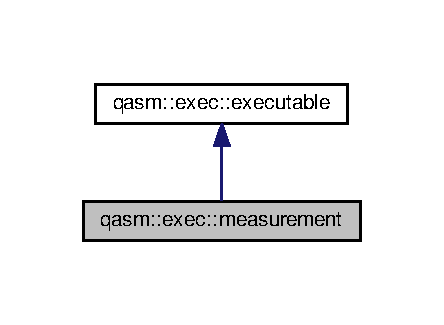
\includegraphics[width=213pt]{classqasm_1_1exec_1_1measurement__inherit__graph}
\end{center}
\end{figure}


Collaboration diagram for qasm\+:\+:exec\+:\+:measurement\+:\nopagebreak
\begin{figure}[H]
\begin{center}
\leavevmode
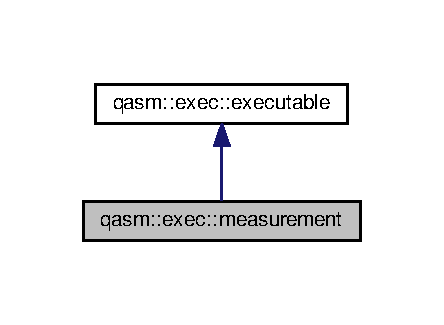
\includegraphics[width=213pt]{classqasm_1_1exec_1_1measurement__coll__graph}
\end{center}
\end{figure}
\subsection*{Public Member Functions}
\begin{DoxyCompactItemize}
\item 
\hyperlink{classqasm_1_1exec_1_1measurement_aea704a014c6ae33420021ec54ab6447b}{measurement} (string qr, long qi, string cr, long ci)
\item 
\hyperlink{classqasm_1_1exec_1_1measurement_a82af9b0d6dea17bd770e8c6e6b5d2fb8}{measurement} (string qr, string cr)
\item 
virtual void \hyperlink{classqasm_1_1exec_1_1measurement_aefa96cf86f31c40a75fbc46924c94bb8}{invoke\+\_\+rootprogram} (\hyperlink{classqasm_1_1runtime_1_1environment}{runtime\+::environment} \&env)
\end{DoxyCompactItemize}
\subsection*{Public Attributes}
\begin{DoxyCompactItemize}
\item 
std\+::string \hyperlink{classqasm_1_1exec_1_1measurement_acd8ed10227ce8755b6449959c508e023}{qreg}
\item 
long \hyperlink{classqasm_1_1exec_1_1measurement_a083137ce86d7f8b1f92a34a2db604063}{qindex}
\item 
std\+::string \hyperlink{classqasm_1_1exec_1_1measurement_a419118b0574b066fdff6c7f00213dec3}{creg}
\item 
long \hyperlink{classqasm_1_1exec_1_1measurement_ab1ba29db121a9c17be8aacbd1f24ff7b}{cindex}
\item 
bool \hyperlink{classqasm_1_1exec_1_1measurement_a1b67bc7f310bcba5a42989229268517d}{measure\+Whole}
\end{DoxyCompactItemize}


\subsection{Detailed Description}
Instruction to measure a quantum variable into a classical one 

\subsection{Constructor \& Destructor Documentation}
\index{qasm\+::exec\+::measurement@{qasm\+::exec\+::measurement}!measurement@{measurement}}
\index{measurement@{measurement}!qasm\+::exec\+::measurement@{qasm\+::exec\+::measurement}}
\subsubsection[{\texorpdfstring{measurement(string qr, long qi, string cr, long ci)}{measurement(string qr, long qi, string cr, long ci)}}]{\setlength{\rightskip}{0pt plus 5cm}qasm\+::exec\+::measurement\+::measurement (
\begin{DoxyParamCaption}
\item[{string}]{qr, }
\item[{long}]{qi, }
\item[{string}]{cr, }
\item[{long}]{ci}
\end{DoxyParamCaption}
)\hspace{0.3cm}{\ttfamily [inline]}}\hypertarget{classqasm_1_1exec_1_1measurement_aea704a014c6ae33420021ec54ab6447b}{}\label{classqasm_1_1exec_1_1measurement_aea704a014c6ae33420021ec54ab6447b}
\index{qasm\+::exec\+::measurement@{qasm\+::exec\+::measurement}!measurement@{measurement}}
\index{measurement@{measurement}!qasm\+::exec\+::measurement@{qasm\+::exec\+::measurement}}
\subsubsection[{\texorpdfstring{measurement(string qr, string cr)}{measurement(string qr, string cr)}}]{\setlength{\rightskip}{0pt plus 5cm}qasm\+::exec\+::measurement\+::measurement (
\begin{DoxyParamCaption}
\item[{string}]{qr, }
\item[{string}]{cr}
\end{DoxyParamCaption}
)\hspace{0.3cm}{\ttfamily [inline]}}\hypertarget{classqasm_1_1exec_1_1measurement_a82af9b0d6dea17bd770e8c6e6b5d2fb8}{}\label{classqasm_1_1exec_1_1measurement_a82af9b0d6dea17bd770e8c6e6b5d2fb8}


\subsection{Member Function Documentation}
\index{qasm\+::exec\+::measurement@{qasm\+::exec\+::measurement}!invoke\+\_\+rootprogram@{invoke\+\_\+rootprogram}}
\index{invoke\+\_\+rootprogram@{invoke\+\_\+rootprogram}!qasm\+::exec\+::measurement@{qasm\+::exec\+::measurement}}
\subsubsection[{\texorpdfstring{invoke\+\_\+rootprogram(runtime\+::environment \&env)}{invoke_rootprogram(runtime::environment &env)}}]{\setlength{\rightskip}{0pt plus 5cm}virtual void qasm\+::exec\+::measurement\+::invoke\+\_\+rootprogram (
\begin{DoxyParamCaption}
\item[{{\bf runtime\+::environment} \&}]{env}
\end{DoxyParamCaption}
)\hspace{0.3cm}{\ttfamily [inline]}, {\ttfamily [virtual]}}\hypertarget{classqasm_1_1exec_1_1measurement_aefa96cf86f31c40a75fbc46924c94bb8}{}\label{classqasm_1_1exec_1_1measurement_aefa96cf86f31c40a75fbc46924c94bb8}
Run instruction\textquotesingle{}s primary operation 

Reimplemented from \hyperlink{classqasm_1_1exec_1_1executable_ad07f864a889edb0777ebbb1bc1628121}{qasm\+::exec\+::executable}.



\subsection{Member Data Documentation}
\index{qasm\+::exec\+::measurement@{qasm\+::exec\+::measurement}!cindex@{cindex}}
\index{cindex@{cindex}!qasm\+::exec\+::measurement@{qasm\+::exec\+::measurement}}
\subsubsection[{\texorpdfstring{cindex}{cindex}}]{\setlength{\rightskip}{0pt plus 5cm}long qasm\+::exec\+::measurement\+::cindex}\hypertarget{classqasm_1_1exec_1_1measurement_ab1ba29db121a9c17be8aacbd1f24ff7b}{}\label{classqasm_1_1exec_1_1measurement_ab1ba29db121a9c17be8aacbd1f24ff7b}
Classic register index \index{qasm\+::exec\+::measurement@{qasm\+::exec\+::measurement}!creg@{creg}}
\index{creg@{creg}!qasm\+::exec\+::measurement@{qasm\+::exec\+::measurement}}
\subsubsection[{\texorpdfstring{creg}{creg}}]{\setlength{\rightskip}{0pt plus 5cm}std\+::string qasm\+::exec\+::measurement\+::creg}\hypertarget{classqasm_1_1exec_1_1measurement_a419118b0574b066fdff6c7f00213dec3}{}\label{classqasm_1_1exec_1_1measurement_a419118b0574b066fdff6c7f00213dec3}
Classic register name \index{qasm\+::exec\+::measurement@{qasm\+::exec\+::measurement}!measure\+Whole@{measure\+Whole}}
\index{measure\+Whole@{measure\+Whole}!qasm\+::exec\+::measurement@{qasm\+::exec\+::measurement}}
\subsubsection[{\texorpdfstring{measure\+Whole}{measureWhole}}]{\setlength{\rightskip}{0pt plus 5cm}bool qasm\+::exec\+::measurement\+::measure\+Whole}\hypertarget{classqasm_1_1exec_1_1measurement_a1b67bc7f310bcba5a42989229268517d}{}\label{classqasm_1_1exec_1_1measurement_a1b67bc7f310bcba5a42989229268517d}
Flag if whole register is to be measured or just the given indexes \index{qasm\+::exec\+::measurement@{qasm\+::exec\+::measurement}!qindex@{qindex}}
\index{qindex@{qindex}!qasm\+::exec\+::measurement@{qasm\+::exec\+::measurement}}
\subsubsection[{\texorpdfstring{qindex}{qindex}}]{\setlength{\rightskip}{0pt plus 5cm}long qasm\+::exec\+::measurement\+::qindex}\hypertarget{classqasm_1_1exec_1_1measurement_a083137ce86d7f8b1f92a34a2db604063}{}\label{classqasm_1_1exec_1_1measurement_a083137ce86d7f8b1f92a34a2db604063}
Quantum register index \index{qasm\+::exec\+::measurement@{qasm\+::exec\+::measurement}!qreg@{qreg}}
\index{qreg@{qreg}!qasm\+::exec\+::measurement@{qasm\+::exec\+::measurement}}
\subsubsection[{\texorpdfstring{qreg}{qreg}}]{\setlength{\rightskip}{0pt plus 5cm}std\+::string qasm\+::exec\+::measurement\+::qreg}\hypertarget{classqasm_1_1exec_1_1measurement_acd8ed10227ce8755b6449959c508e023}{}\label{classqasm_1_1exec_1_1measurement_acd8ed10227ce8755b6449959c508e023}
Quantum register name 

The documentation for this class was generated from the following file\+:\begin{DoxyCompactItemize}
\item 
src/runtime/\hyperlink{runtime_8hpp}{runtime.\+hpp}\end{DoxyCompactItemize}

\hypertarget{classqlib_1_1quantum_1_1gates_1_1onequbitgate}{}\section{qlib\+:\+:quantum\+:\+:gates\+:\+:onequbitgate Class Reference}
\label{classqlib_1_1quantum_1_1gates_1_1onequbitgate}\index{qlib\+::quantum\+::gates\+::onequbitgate@{qlib\+::quantum\+::gates\+::onequbitgate}}


{\ttfamily \#include $<$onequbitgate.\+hpp$>$}



Inheritance diagram for qlib\+:\+:quantum\+:\+:gates\+:\+:onequbitgate\+:\nopagebreak
\begin{figure}[H]
\begin{center}
\leavevmode
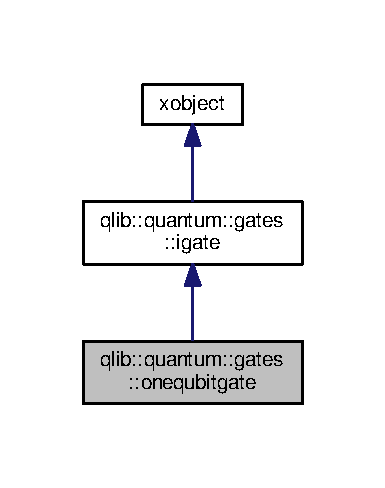
\includegraphics[width=185pt]{classqlib_1_1quantum_1_1gates_1_1onequbitgate__inherit__graph}
\end{center}
\end{figure}


Collaboration diagram for qlib\+:\+:quantum\+:\+:gates\+:\+:onequbitgate\+:\nopagebreak
\begin{figure}[H]
\begin{center}
\leavevmode
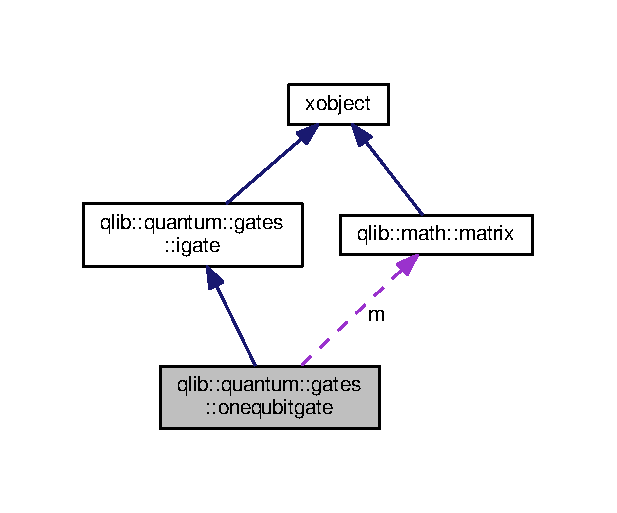
\includegraphics[width=296pt]{classqlib_1_1quantum_1_1gates_1_1onequbitgate__coll__graph}
\end{center}
\end{figure}
\subsection*{Public Member Functions}
\begin{DoxyCompactItemize}
\item 
\hyperlink{classqlib_1_1quantum_1_1gates_1_1onequbitgate_a587ebdfa032f58bf63433c89c6015149}{onequbitgate} (std\+::string \hyperlink{classqlib_1_1quantum_1_1gates_1_1onequbitgate_aacf3878010f0c1327bae4dcc7faf4c92}{name}, std\+::vector$<$ \hyperlink{classqlib_1_1math_1_1complex}{complex} $>$ values)
\item 
size\+\_\+t \hyperlink{classqlib_1_1quantum_1_1gates_1_1onequbitgate_a050ed71ebff89050c3123124f8ba8719}{inputs} ()
\item 
std\+::string \hyperlink{classqlib_1_1quantum_1_1gates_1_1onequbitgate_aacf3878010f0c1327bae4dcc7faf4c92}{name} ()
\item 
void \hyperlink{classqlib_1_1quantum_1_1gates_1_1onequbitgate_a280c7a7d29032eeb95afcb3d6668e7db}{operate} (\hyperlink{classqlib_1_1math_1_1matrix}{matrix} \&in, \hyperlink{classqlib_1_1math_1_1matrix}{matrix} \&out, std\+::vector$<$ u64 $>$ input\+Qubits)
\item 
\hyperlink{classqlib_1_1math_1_1matrix}{qlib\+::math\+::matrix} \& \hyperlink{classqlib_1_1quantum_1_1gates_1_1onequbitgate_a39490c6d1dcc94dc82bb7345fe984278}{get\+Matrix} ()
\item 
std\+::string \hyperlink{classqlib_1_1quantum_1_1gates_1_1onequbitgate_a38af1af0f466add047c3e75780e28c80}{to\+String} ()
\end{DoxyCompactItemize}
\subsection*{Private Attributes}
\begin{DoxyCompactItemize}
\item 
std\+::string \hyperlink{classqlib_1_1quantum_1_1gates_1_1onequbitgate_abc5ac874b8a4174cc72a159d3c6d91d2}{sname}
\item 
\hyperlink{classqlib_1_1math_1_1matrix}{matrix} \hyperlink{classqlib_1_1quantum_1_1gates_1_1onequbitgate_a6d935a1219c646b16c136560a5b4f0bf}{m}
\end{DoxyCompactItemize}


\subsection{Constructor \& Destructor Documentation}
\index{qlib\+::quantum\+::gates\+::onequbitgate@{qlib\+::quantum\+::gates\+::onequbitgate}!onequbitgate@{onequbitgate}}
\index{onequbitgate@{onequbitgate}!qlib\+::quantum\+::gates\+::onequbitgate@{qlib\+::quantum\+::gates\+::onequbitgate}}
\subsubsection[{\texorpdfstring{onequbitgate(std\+::string name, std\+::vector$<$ complex $>$ values)}{onequbitgate(std::string name, std::vector< complex > values)}}]{\setlength{\rightskip}{0pt plus 5cm}qlib\+::quantum\+::gates\+::onequbitgate\+::onequbitgate (
\begin{DoxyParamCaption}
\item[{std\+::string}]{name, }
\item[{std\+::vector$<$ {\bf complex} $>$}]{values}
\end{DoxyParamCaption}
)\hspace{0.3cm}{\ttfamily [inline]}}\hypertarget{classqlib_1_1quantum_1_1gates_1_1onequbitgate_a587ebdfa032f58bf63433c89c6015149}{}\label{classqlib_1_1quantum_1_1gates_1_1onequbitgate_a587ebdfa032f58bf63433c89c6015149}
Create a new quanutm operator for the given number of states 

\subsection{Member Function Documentation}
\index{qlib\+::quantum\+::gates\+::onequbitgate@{qlib\+::quantum\+::gates\+::onequbitgate}!get\+Matrix@{get\+Matrix}}
\index{get\+Matrix@{get\+Matrix}!qlib\+::quantum\+::gates\+::onequbitgate@{qlib\+::quantum\+::gates\+::onequbitgate}}
\subsubsection[{\texorpdfstring{get\+Matrix()}{getMatrix()}}]{\setlength{\rightskip}{0pt plus 5cm}{\bf qlib\+::math\+::matrix}\& qlib\+::quantum\+::gates\+::onequbitgate\+::get\+Matrix (
\begin{DoxyParamCaption}
{}
\end{DoxyParamCaption}
)\hspace{0.3cm}{\ttfamily [inline]}}\hypertarget{classqlib_1_1quantum_1_1gates_1_1onequbitgate_a39490c6d1dcc94dc82bb7345fe984278}{}\label{classqlib_1_1quantum_1_1gates_1_1onequbitgate_a39490c6d1dcc94dc82bb7345fe984278}
Returns the matrix representation of this operator \index{qlib\+::quantum\+::gates\+::onequbitgate@{qlib\+::quantum\+::gates\+::onequbitgate}!inputs@{inputs}}
\index{inputs@{inputs}!qlib\+::quantum\+::gates\+::onequbitgate@{qlib\+::quantum\+::gates\+::onequbitgate}}
\subsubsection[{\texorpdfstring{inputs()}{inputs()}}]{\setlength{\rightskip}{0pt plus 5cm}size\+\_\+t qlib\+::quantum\+::gates\+::onequbitgate\+::inputs (
\begin{DoxyParamCaption}
{}
\end{DoxyParamCaption}
)\hspace{0.3cm}{\ttfamily [inline]}, {\ttfamily [virtual]}}\hypertarget{classqlib_1_1quantum_1_1gates_1_1onequbitgate_a050ed71ebff89050c3123124f8ba8719}{}\label{classqlib_1_1quantum_1_1gates_1_1onequbitgate_a050ed71ebff89050c3123124f8ba8719}
Number of input qubits this operator can be applied to 

Implements \hyperlink{classqlib_1_1quantum_1_1gates_1_1igate_ac8aa56b0095a94fdd437bc55d90aec9d}{qlib\+::quantum\+::gates\+::igate}.

\index{qlib\+::quantum\+::gates\+::onequbitgate@{qlib\+::quantum\+::gates\+::onequbitgate}!name@{name}}
\index{name@{name}!qlib\+::quantum\+::gates\+::onequbitgate@{qlib\+::quantum\+::gates\+::onequbitgate}}
\subsubsection[{\texorpdfstring{name()}{name()}}]{\setlength{\rightskip}{0pt plus 5cm}std\+::string qlib\+::quantum\+::gates\+::onequbitgate\+::name (
\begin{DoxyParamCaption}
{}
\end{DoxyParamCaption}
)\hspace{0.3cm}{\ttfamily [inline]}, {\ttfamily [virtual]}}\hypertarget{classqlib_1_1quantum_1_1gates_1_1onequbitgate_aacf3878010f0c1327bae4dcc7faf4c92}{}\label{classqlib_1_1quantum_1_1gates_1_1onequbitgate_aacf3878010f0c1327bae4dcc7faf4c92}
The name of this gate 

Implements \hyperlink{classqlib_1_1quantum_1_1gates_1_1igate_ae8f8dda69d7742c12c743829abb3662b}{qlib\+::quantum\+::gates\+::igate}.

\index{qlib\+::quantum\+::gates\+::onequbitgate@{qlib\+::quantum\+::gates\+::onequbitgate}!operate@{operate}}
\index{operate@{operate}!qlib\+::quantum\+::gates\+::onequbitgate@{qlib\+::quantum\+::gates\+::onequbitgate}}
\subsubsection[{\texorpdfstring{operate(matrix \&in, matrix \&out, std\+::vector$<$ u64 $>$ input\+Qubits)}{operate(matrix &in, matrix &out, std::vector< u64 > inputQubits)}}]{\setlength{\rightskip}{0pt plus 5cm}void qlib\+::quantum\+::gates\+::onequbitgate\+::operate (
\begin{DoxyParamCaption}
\item[{{\bf matrix} \&}]{in, }
\item[{{\bf matrix} \&}]{out, }
\item[{std\+::vector$<$ u64 $>$}]{input\+Qubits}
\end{DoxyParamCaption}
)\hspace{0.3cm}{\ttfamily [inline]}, {\ttfamily [virtual]}}\hypertarget{classqlib_1_1quantum_1_1gates_1_1onequbitgate_a280c7a7d29032eeb95afcb3d6668e7db}{}\label{classqlib_1_1quantum_1_1gates_1_1onequbitgate_a280c7a7d29032eeb95afcb3d6668e7db}
Operate on a given column vector state superposition 

Implements \hyperlink{classqlib_1_1quantum_1_1gates_1_1igate_a66038ee65fec12c627789505e11f1e23}{qlib\+::quantum\+::gates\+::igate}.

\index{qlib\+::quantum\+::gates\+::onequbitgate@{qlib\+::quantum\+::gates\+::onequbitgate}!to\+String@{to\+String}}
\index{to\+String@{to\+String}!qlib\+::quantum\+::gates\+::onequbitgate@{qlib\+::quantum\+::gates\+::onequbitgate}}
\subsubsection[{\texorpdfstring{to\+String()}{toString()}}]{\setlength{\rightskip}{0pt plus 5cm}std\+::string qlib\+::quantum\+::gates\+::onequbitgate\+::to\+String (
\begin{DoxyParamCaption}
{}
\end{DoxyParamCaption}
)\hspace{0.3cm}{\ttfamily [inline]}, {\ttfamily [virtual]}}\hypertarget{classqlib_1_1quantum_1_1gates_1_1onequbitgate_a38af1af0f466add047c3e75780e28c80}{}\label{classqlib_1_1quantum_1_1gates_1_1onequbitgate_a38af1af0f466add047c3e75780e28c80}
Pretty print 

Reimplemented from \hyperlink{classxobject_ad76243a44c4e4959d3b16bb57d82600d}{xobject}.



\subsection{Member Data Documentation}
\index{qlib\+::quantum\+::gates\+::onequbitgate@{qlib\+::quantum\+::gates\+::onequbitgate}!m@{m}}
\index{m@{m}!qlib\+::quantum\+::gates\+::onequbitgate@{qlib\+::quantum\+::gates\+::onequbitgate}}
\subsubsection[{\texorpdfstring{m}{m}}]{\setlength{\rightskip}{0pt plus 5cm}{\bf matrix} qlib\+::quantum\+::gates\+::onequbitgate\+::m\hspace{0.3cm}{\ttfamily [private]}}\hypertarget{classqlib_1_1quantum_1_1gates_1_1onequbitgate_a6d935a1219c646b16c136560a5b4f0bf}{}\label{classqlib_1_1quantum_1_1gates_1_1onequbitgate_a6d935a1219c646b16c136560a5b4f0bf}
\index{qlib\+::quantum\+::gates\+::onequbitgate@{qlib\+::quantum\+::gates\+::onequbitgate}!sname@{sname}}
\index{sname@{sname}!qlib\+::quantum\+::gates\+::onequbitgate@{qlib\+::quantum\+::gates\+::onequbitgate}}
\subsubsection[{\texorpdfstring{sname}{sname}}]{\setlength{\rightskip}{0pt plus 5cm}std\+::string qlib\+::quantum\+::gates\+::onequbitgate\+::sname\hspace{0.3cm}{\ttfamily [private]}}\hypertarget{classqlib_1_1quantum_1_1gates_1_1onequbitgate_abc5ac874b8a4174cc72a159d3c6d91d2}{}\label{classqlib_1_1quantum_1_1gates_1_1onequbitgate_abc5ac874b8a4174cc72a159d3c6d91d2}


The documentation for this class was generated from the following file\+:\begin{DoxyCompactItemize}
\item 
src/core/quantum/gates/\hyperlink{onequbitgate_8hpp}{onequbitgate.\+hpp}\end{DoxyCompactItemize}

\hypertarget{classqlib_1_1ide_1_1OptionsMenu}{}\section{qlib.\+ide.\+Options\+Menu Class Reference}
\label{classqlib_1_1ide_1_1OptionsMenu}\index{qlib.\+ide.\+Options\+Menu@{qlib.\+ide.\+Options\+Menu}}


Inheritance diagram for qlib.\+ide.\+Options\+Menu\+:
\nopagebreak
\begin{figure}[H]
\begin{center}
\leavevmode
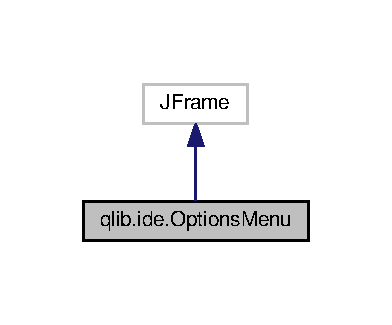
\includegraphics[width=188pt]{classqlib_1_1ide_1_1OptionsMenu__inherit__graph}
\end{center}
\end{figure}


Collaboration diagram for qlib.\+ide.\+Options\+Menu\+:
\nopagebreak
\begin{figure}[H]
\begin{center}
\leavevmode
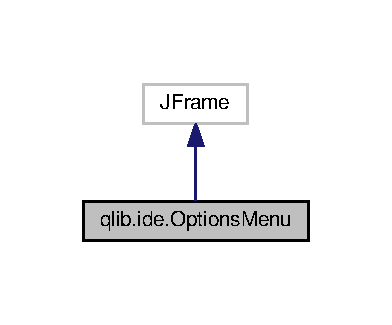
\includegraphics[width=188pt]{classqlib_1_1ide_1_1OptionsMenu__coll__graph}
\end{center}
\end{figure}
\subsection*{Public Member Functions}
\begin{DoxyCompactItemize}
\item 
\hyperlink{classqlib_1_1ide_1_1OptionsMenu_a51481ab49936fea97fbf021ae7b37a13}{Options\+Menu} (\hyperlink{classqlib_1_1ide_1_1IniIO}{Ini\+IO} ini, String config\+\_\+path)
\end{DoxyCompactItemize}


\subsection{Detailed Description}
J\+Frame with a table for modifying key-\/value pairs in an I\+NI file \begin{DoxyAuthor}{Author}
halse 
\end{DoxyAuthor}


\subsection{Constructor \& Destructor Documentation}
\index{qlib\+::ide\+::\+Options\+Menu@{qlib\+::ide\+::\+Options\+Menu}!Options\+Menu@{Options\+Menu}}
\index{Options\+Menu@{Options\+Menu}!qlib\+::ide\+::\+Options\+Menu@{qlib\+::ide\+::\+Options\+Menu}}
\subsubsection[{\texorpdfstring{Options\+Menu(\+Ini\+I\+O ini, String config\+\_\+path)}{OptionsMenu(IniIO ini, String config_path)}}]{\setlength{\rightskip}{0pt plus 5cm}qlib.\+ide.\+Options\+Menu.\+Options\+Menu (
\begin{DoxyParamCaption}
\item[{{\bf Ini\+IO}}]{ini, }
\item[{String}]{config\+\_\+path}
\end{DoxyParamCaption}
)\hspace{0.3cm}{\ttfamily [inline]}}\hypertarget{classqlib_1_1ide_1_1OptionsMenu_a51481ab49936fea97fbf021ae7b37a13}{}\label{classqlib_1_1ide_1_1OptionsMenu_a51481ab49936fea97fbf021ae7b37a13}


The documentation for this class was generated from the following file\+:\begin{DoxyCompactItemize}
\item 
src/ide/src/qlib/ide/\hyperlink{OptionsMenu_8java}{Options\+Menu.\+java}\end{DoxyCompactItemize}

\hypertarget{classparseexception}{}\section{parseexception Class Reference}
\label{classparseexception}\index{parseexception@{parseexception}}


{\ttfamily \#include $<$qasmparser.\+hpp$>$}



Inheritance diagram for parseexception\+:\nopagebreak
\begin{figure}[H]
\begin{center}
\leavevmode
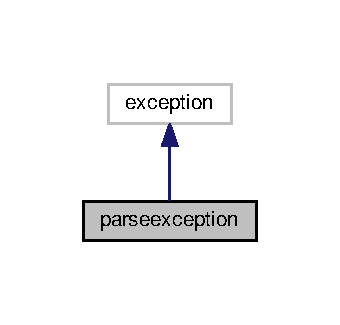
\includegraphics[width=163pt]{classparseexception__inherit__graph}
\end{center}
\end{figure}


Collaboration diagram for parseexception\+:\nopagebreak
\begin{figure}[H]
\begin{center}
\leavevmode
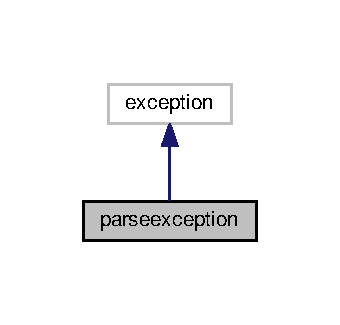
\includegraphics[width=163pt]{classparseexception__coll__graph}
\end{center}
\end{figure}
\subsection*{Public Member Functions}
\begin{DoxyCompactItemize}
\item 
\hyperlink{classparseexception_a16accd5bc62f4465b611b38db6751e0e}{parseexception} (\hyperlink{types_8h_ab2bb0e5480d1d957383df6b350794313}{ulong} row, \hyperlink{types_8h_ab2bb0e5480d1d957383df6b350794313}{ulong} column, std\+::string \hyperlink{classparseexception_a99a096bfed3e48cd365cdae1952bc017}{file}, std\+::string message)
\item 
const char $\ast$ \hyperlink{classparseexception_a006c6421028f780b91eb4a473265dce7}{what} () const   throw ()
\end{DoxyCompactItemize}
\subsection*{Public Attributes}
\begin{DoxyCompactItemize}
\item 
\hyperlink{types_8h_ab2bb0e5480d1d957383df6b350794313}{ulong} \hyperlink{classparseexception_a0e50402f7511e71332099355061b26ca}{r}
\item 
\hyperlink{types_8h_ab2bb0e5480d1d957383df6b350794313}{ulong} \hyperlink{classparseexception_a671840c0e1441210c84084e235fa55c8}{c}
\item 
std\+::string \hyperlink{classparseexception_a99a096bfed3e48cd365cdae1952bc017}{file}
\item 
std\+::string \hyperlink{classparseexception_a5f02ff7145f65ba4e9b5be994bfc0edb}{msg}
\end{DoxyCompactItemize}
\subsection*{Private Attributes}
\begin{DoxyCompactItemize}
\item 
std\+::string \hyperlink{classparseexception_a4807889c64609ea29a275c9f66c15e61}{what\+\_\+message}
\end{DoxyCompactItemize}


\subsection{Detailed Description}
Class for exceptions occuring during parsing of lexical tokens 

\subsection{Constructor \& Destructor Documentation}
\index{parseexception@{parseexception}!parseexception@{parseexception}}
\index{parseexception@{parseexception}!parseexception@{parseexception}}
\subsubsection[{\texorpdfstring{parseexception(ulong row, ulong column, std\+::string file, std\+::string message)}{parseexception(ulong row, ulong column, std::string file, std::string message)}}]{\setlength{\rightskip}{0pt plus 5cm}parseexception\+::parseexception (
\begin{DoxyParamCaption}
\item[{{\bf ulong}}]{row, }
\item[{{\bf ulong}}]{column, }
\item[{std\+::string}]{file, }
\item[{std\+::string}]{message}
\end{DoxyParamCaption}
)\hspace{0.3cm}{\ttfamily [inline]}}\hypertarget{classparseexception_a16accd5bc62f4465b611b38db6751e0e}{}\label{classparseexception_a16accd5bc62f4465b611b38db6751e0e}


\subsection{Member Function Documentation}
\index{parseexception@{parseexception}!what@{what}}
\index{what@{what}!parseexception@{parseexception}}
\subsubsection[{\texorpdfstring{what() const }{what() const }}]{\setlength{\rightskip}{0pt plus 5cm}const char$\ast$ parseexception\+::what (
\begin{DoxyParamCaption}
{}
\end{DoxyParamCaption}
) const throw  ) \hspace{0.3cm}{\ttfamily [inline]}}\hypertarget{classparseexception_a006c6421028f780b91eb4a473265dce7}{}\label{classparseexception_a006c6421028f780b91eb4a473265dce7}


\subsection{Member Data Documentation}
\index{parseexception@{parseexception}!c@{c}}
\index{c@{c}!parseexception@{parseexception}}
\subsubsection[{\texorpdfstring{c}{c}}]{\setlength{\rightskip}{0pt plus 5cm}{\bf ulong} parseexception\+::c}\hypertarget{classparseexception_a671840c0e1441210c84084e235fa55c8}{}\label{classparseexception_a671840c0e1441210c84084e235fa55c8}
Column of cause \index{parseexception@{parseexception}!file@{file}}
\index{file@{file}!parseexception@{parseexception}}
\subsubsection[{\texorpdfstring{file}{file}}]{\setlength{\rightskip}{0pt plus 5cm}std\+::string parseexception\+::file}\hypertarget{classparseexception_a99a096bfed3e48cd365cdae1952bc017}{}\label{classparseexception_a99a096bfed3e48cd365cdae1952bc017}
Filename cause occurred in \index{parseexception@{parseexception}!msg@{msg}}
\index{msg@{msg}!parseexception@{parseexception}}
\subsubsection[{\texorpdfstring{msg}{msg}}]{\setlength{\rightskip}{0pt plus 5cm}std\+::string parseexception\+::msg}\hypertarget{classparseexception_a5f02ff7145f65ba4e9b5be994bfc0edb}{}\label{classparseexception_a5f02ff7145f65ba4e9b5be994bfc0edb}
Cause of exception \index{parseexception@{parseexception}!r@{r}}
\index{r@{r}!parseexception@{parseexception}}
\subsubsection[{\texorpdfstring{r}{r}}]{\setlength{\rightskip}{0pt plus 5cm}{\bf ulong} parseexception\+::r}\hypertarget{classparseexception_a0e50402f7511e71332099355061b26ca}{}\label{classparseexception_a0e50402f7511e71332099355061b26ca}
Row of cause \index{parseexception@{parseexception}!what\+\_\+message@{what\+\_\+message}}
\index{what\+\_\+message@{what\+\_\+message}!parseexception@{parseexception}}
\subsubsection[{\texorpdfstring{what\+\_\+message}{what_message}}]{\setlength{\rightskip}{0pt plus 5cm}std\+::string parseexception\+::what\+\_\+message\hspace{0.3cm}{\ttfamily [private]}}\hypertarget{classparseexception_a4807889c64609ea29a275c9f66c15e61}{}\label{classparseexception_a4807889c64609ea29a275c9f66c15e61}
Combined message 

The documentation for this class was generated from the following file\+:\begin{DoxyCompactItemize}
\item 
src/runtime/\hyperlink{qasmparser_8hpp}{qasmparser.\+hpp}\end{DoxyCompactItemize}

\hypertarget{structparser_1_1parsetree}{}\section{parser\+:\+:parsetree Struct Reference}
\label{structparser_1_1parsetree}\index{parser\+::parsetree@{parser\+::parsetree}}


{\ttfamily \#include $<$parser.\+hpp$>$}



Collaboration diagram for parser\+:\+:parsetree\+:\nopagebreak
\begin{figure}[H]
\begin{center}
\leavevmode
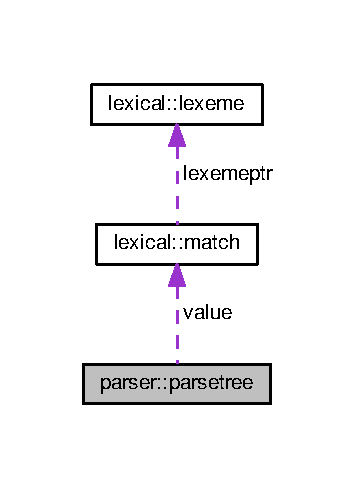
\includegraphics[width=171pt]{structparser_1_1parsetree__coll__graph}
\end{center}
\end{figure}
\subsection*{Public Member Functions}
\begin{DoxyCompactItemize}
\item 
bool \hyperlink{structparser_1_1parsetree_a8ba2bf7b05dd8e858edf2fab9f3d0165}{is\+Leaf} ()
\item 
bool \hyperlink{structparser_1_1parsetree_a2e876beca6bc762fa2ecb849f681f311}{is\+Branch} ()
\item 
bool \hyperlink{structparser_1_1parsetree_a460a38e7e9a33cafe00c7f7b2163f75a}{is\+Binary} ()
\item 
\hyperlink{structparser_1_1parsetree}{parsetree} \& \hyperlink{structparser_1_1parsetree_a74fd9e1633a6581f3c07a6263a686bd3}{get\+Left} ()
\item 
\hyperlink{structparser_1_1parsetree}{parsetree} \& \hyperlink{structparser_1_1parsetree_a3f158cea846ac57f787eb81a9ac2477f}{get\+Right} ()
\item 
size\+\_\+t \hyperlink{structparser_1_1parsetree_a791b5113d65303aa8d272b0eb749cb54}{size} ()
\item 
\hyperlink{structparser_1_1parsetree}{parsetree} \& \hyperlink{structparser_1_1parsetree_af238368fcc40aea999cab62ba7d74fda}{get\+Child} (size\+\_\+t i)
\item 
void \hyperlink{structparser_1_1parsetree_ada59e97da6280e95cf96cbb8f85df364}{print} ()
\end{DoxyCompactItemize}
\subsection*{Public Attributes}
\begin{DoxyCompactItemize}
\item 
\hyperlink{structlexical_1_1match}{match} \hyperlink{structparser_1_1parsetree_a4ee1d9214dd2a25fcf0494afaa9be7d7}{value}
\item 
vector$<$ \hyperlink{structparser_1_1parsetree}{parsetree} $>$ \hyperlink{structparser_1_1parsetree_a46c4ae92fc6d3fb1ac7cbe2827728149}{children}
\end{DoxyCompactItemize}


\subsection{Detailed Description}
Class representing a single node in an abstract tree structure 

\subsection{Member Function Documentation}
\index{parser\+::parsetree@{parser\+::parsetree}!get\+Child@{get\+Child}}
\index{get\+Child@{get\+Child}!parser\+::parsetree@{parser\+::parsetree}}
\subsubsection[{\texorpdfstring{get\+Child(size\+\_\+t i)}{getChild(size_t i)}}]{\setlength{\rightskip}{0pt plus 5cm}{\bf parsetree}\& parser\+::parsetree\+::get\+Child (
\begin{DoxyParamCaption}
\item[{size\+\_\+t}]{i}
\end{DoxyParamCaption}
)\hspace{0.3cm}{\ttfamily [inline]}}\hypertarget{structparser_1_1parsetree_af238368fcc40aea999cab62ba7d74fda}{}\label{structparser_1_1parsetree_af238368fcc40aea999cab62ba7d74fda}
Get a specific child element \index{parser\+::parsetree@{parser\+::parsetree}!get\+Left@{get\+Left}}
\index{get\+Left@{get\+Left}!parser\+::parsetree@{parser\+::parsetree}}
\subsubsection[{\texorpdfstring{get\+Left()}{getLeft()}}]{\setlength{\rightskip}{0pt plus 5cm}{\bf parsetree}\& parser\+::parsetree\+::get\+Left (
\begin{DoxyParamCaption}
{}
\end{DoxyParamCaption}
)\hspace{0.3cm}{\ttfamily [inline]}}\hypertarget{structparser_1_1parsetree_a74fd9e1633a6581f3c07a6263a686bd3}{}\label{structparser_1_1parsetree_a74fd9e1633a6581f3c07a6263a686bd3}
If tree is binary, get the left hand child (index 0) \index{parser\+::parsetree@{parser\+::parsetree}!get\+Right@{get\+Right}}
\index{get\+Right@{get\+Right}!parser\+::parsetree@{parser\+::parsetree}}
\subsubsection[{\texorpdfstring{get\+Right()}{getRight()}}]{\setlength{\rightskip}{0pt plus 5cm}{\bf parsetree}\& parser\+::parsetree\+::get\+Right (
\begin{DoxyParamCaption}
{}
\end{DoxyParamCaption}
)\hspace{0.3cm}{\ttfamily [inline]}}\hypertarget{structparser_1_1parsetree_a3f158cea846ac57f787eb81a9ac2477f}{}\label{structparser_1_1parsetree_a3f158cea846ac57f787eb81a9ac2477f}
If tree is binary, get the right hand child (index 1) \index{parser\+::parsetree@{parser\+::parsetree}!is\+Binary@{is\+Binary}}
\index{is\+Binary@{is\+Binary}!parser\+::parsetree@{parser\+::parsetree}}
\subsubsection[{\texorpdfstring{is\+Binary()}{isBinary()}}]{\setlength{\rightskip}{0pt plus 5cm}bool parser\+::parsetree\+::is\+Binary (
\begin{DoxyParamCaption}
{}
\end{DoxyParamCaption}
)\hspace{0.3cm}{\ttfamily [inline]}}\hypertarget{structparser_1_1parsetree_a460a38e7e9a33cafe00c7f7b2163f75a}{}\label{structparser_1_1parsetree_a460a38e7e9a33cafe00c7f7b2163f75a}
Test if the parse tree node is binary \index{parser\+::parsetree@{parser\+::parsetree}!is\+Branch@{is\+Branch}}
\index{is\+Branch@{is\+Branch}!parser\+::parsetree@{parser\+::parsetree}}
\subsubsection[{\texorpdfstring{is\+Branch()}{isBranch()}}]{\setlength{\rightskip}{0pt plus 5cm}bool parser\+::parsetree\+::is\+Branch (
\begin{DoxyParamCaption}
{}
\end{DoxyParamCaption}
)\hspace{0.3cm}{\ttfamily [inline]}}\hypertarget{structparser_1_1parsetree_a2e876beca6bc762fa2ecb849f681f311}{}\label{structparser_1_1parsetree_a2e876beca6bc762fa2ecb849f681f311}
Check if node has children \index{parser\+::parsetree@{parser\+::parsetree}!is\+Leaf@{is\+Leaf}}
\index{is\+Leaf@{is\+Leaf}!parser\+::parsetree@{parser\+::parsetree}}
\subsubsection[{\texorpdfstring{is\+Leaf()}{isLeaf()}}]{\setlength{\rightskip}{0pt plus 5cm}bool parser\+::parsetree\+::is\+Leaf (
\begin{DoxyParamCaption}
{}
\end{DoxyParamCaption}
)\hspace{0.3cm}{\ttfamily [inline]}}\hypertarget{structparser_1_1parsetree_a8ba2bf7b05dd8e858edf2fab9f3d0165}{}\label{structparser_1_1parsetree_a8ba2bf7b05dd8e858edf2fab9f3d0165}
Check if node has no children \index{parser\+::parsetree@{parser\+::parsetree}!print@{print}}
\index{print@{print}!parser\+::parsetree@{parser\+::parsetree}}
\subsubsection[{\texorpdfstring{print()}{print()}}]{\setlength{\rightskip}{0pt plus 5cm}void parser\+::parsetree\+::print (
\begin{DoxyParamCaption}
{}
\end{DoxyParamCaption}
)\hspace{0.3cm}{\ttfamily [inline]}}\hypertarget{structparser_1_1parsetree_ada59e97da6280e95cf96cbb8f85df364}{}\label{structparser_1_1parsetree_ada59e97da6280e95cf96cbb8f85df364}
Print tree to standard out, usefull in debugging \index{parser\+::parsetree@{parser\+::parsetree}!size@{size}}
\index{size@{size}!parser\+::parsetree@{parser\+::parsetree}}
\subsubsection[{\texorpdfstring{size()}{size()}}]{\setlength{\rightskip}{0pt plus 5cm}size\+\_\+t parser\+::parsetree\+::size (
\begin{DoxyParamCaption}
{}
\end{DoxyParamCaption}
)\hspace{0.3cm}{\ttfamily [inline]}}\hypertarget{structparser_1_1parsetree_a791b5113d65303aa8d272b0eb749cb54}{}\label{structparser_1_1parsetree_a791b5113d65303aa8d272b0eb749cb54}
Number of children elements 

\subsection{Member Data Documentation}
\index{parser\+::parsetree@{parser\+::parsetree}!children@{children}}
\index{children@{children}!parser\+::parsetree@{parser\+::parsetree}}
\subsubsection[{\texorpdfstring{children}{children}}]{\setlength{\rightskip}{0pt plus 5cm}vector$<${\bf parsetree}$>$ parser\+::parsetree\+::children}\hypertarget{structparser_1_1parsetree_a46c4ae92fc6d3fb1ac7cbe2827728149}{}\label{structparser_1_1parsetree_a46c4ae92fc6d3fb1ac7cbe2827728149}
Children of this node (usually 2) \index{parser\+::parsetree@{parser\+::parsetree}!value@{value}}
\index{value@{value}!parser\+::parsetree@{parser\+::parsetree}}
\subsubsection[{\texorpdfstring{value}{value}}]{\setlength{\rightskip}{0pt plus 5cm}{\bf match} parser\+::parsetree\+::value}\hypertarget{structparser_1_1parsetree_a4ee1d9214dd2a25fcf0494afaa9be7d7}{}\label{structparser_1_1parsetree_a4ee1d9214dd2a25fcf0494afaa9be7d7}
Lexical match associated with this node 

The documentation for this struct was generated from the following file\+:\begin{DoxyCompactItemize}
\item 
src/runtime/\hyperlink{parser_8hpp}{parser.\+hpp}\end{DoxyCompactItemize}

\hypertarget{classqasm_1_1exec_1_1print}{}\section{qasm\+:\+:exec\+:\+:print Class Reference}
\label{classqasm_1_1exec_1_1print}\index{qasm\+::exec\+::print@{qasm\+::exec\+::print}}


{\ttfamily \#include $<$runtime.\+hpp$>$}



Inheritance diagram for qasm\+:\+:exec\+:\+:print\+:\nopagebreak
\begin{figure}[H]
\begin{center}
\leavevmode
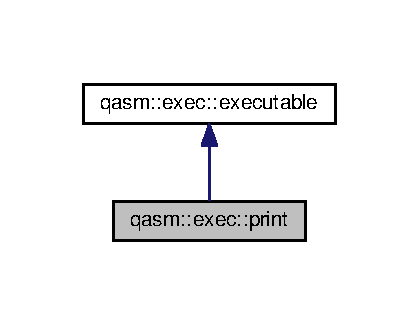
\includegraphics[width=201pt]{classqasm_1_1exec_1_1print__inherit__graph}
\end{center}
\end{figure}


Collaboration diagram for qasm\+:\+:exec\+:\+:print\+:\nopagebreak
\begin{figure}[H]
\begin{center}
\leavevmode
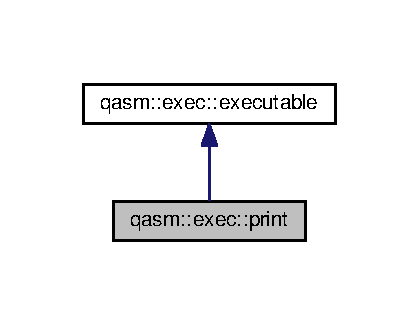
\includegraphics[width=201pt]{classqasm_1_1exec_1_1print__coll__graph}
\end{center}
\end{figure}
\subsection*{Public Member Functions}
\begin{DoxyCompactItemize}
\item 
\hyperlink{classqasm_1_1exec_1_1print_ac6a07cc31446b99250263e748ac0c60d}{print} (string ref)
\item 
virtual void \hyperlink{classqasm_1_1exec_1_1print_ae803c9f70d2a1afd3bbe6e0520e9678b}{invoke\+\_\+rootprogram} (\hyperlink{classqasm_1_1runtime_1_1environment}{runtime\+::environment} \&env)
\end{DoxyCompactItemize}
\subsection*{Public Attributes}
\begin{DoxyCompactItemize}
\item 
std\+::string \hyperlink{classqasm_1_1exec_1_1print_a8d2e5bc3ca543419f7270f97fea27b9b}{reference}
\end{DoxyCompactItemize}


\subsection{Detailed Description}
Instruction to print register to console 

\subsection{Constructor \& Destructor Documentation}
\index{qasm\+::exec\+::print@{qasm\+::exec\+::print}!print@{print}}
\index{print@{print}!qasm\+::exec\+::print@{qasm\+::exec\+::print}}
\subsubsection[{\texorpdfstring{print(string ref)}{print(string ref)}}]{\setlength{\rightskip}{0pt plus 5cm}qasm\+::exec\+::print\+::print (
\begin{DoxyParamCaption}
\item[{string}]{ref}
\end{DoxyParamCaption}
)\hspace{0.3cm}{\ttfamily [inline]}}\hypertarget{classqasm_1_1exec_1_1print_ac6a07cc31446b99250263e748ac0c60d}{}\label{classqasm_1_1exec_1_1print_ac6a07cc31446b99250263e748ac0c60d}


\subsection{Member Function Documentation}
\index{qasm\+::exec\+::print@{qasm\+::exec\+::print}!invoke\+\_\+rootprogram@{invoke\+\_\+rootprogram}}
\index{invoke\+\_\+rootprogram@{invoke\+\_\+rootprogram}!qasm\+::exec\+::print@{qasm\+::exec\+::print}}
\subsubsection[{\texorpdfstring{invoke\+\_\+rootprogram(runtime\+::environment \&env)}{invoke_rootprogram(runtime::environment &env)}}]{\setlength{\rightskip}{0pt plus 5cm}virtual void qasm\+::exec\+::print\+::invoke\+\_\+rootprogram (
\begin{DoxyParamCaption}
\item[{{\bf runtime\+::environment} \&}]{env}
\end{DoxyParamCaption}
)\hspace{0.3cm}{\ttfamily [inline]}, {\ttfamily [virtual]}}\hypertarget{classqasm_1_1exec_1_1print_ae803c9f70d2a1afd3bbe6e0520e9678b}{}\label{classqasm_1_1exec_1_1print_ae803c9f70d2a1afd3bbe6e0520e9678b}
Run instruction\textquotesingle{}s primary operation 

Reimplemented from \hyperlink{classqasm_1_1exec_1_1executable_ad07f864a889edb0777ebbb1bc1628121}{qasm\+::exec\+::executable}.



\subsection{Member Data Documentation}
\index{qasm\+::exec\+::print@{qasm\+::exec\+::print}!reference@{reference}}
\index{reference@{reference}!qasm\+::exec\+::print@{qasm\+::exec\+::print}}
\subsubsection[{\texorpdfstring{reference}{reference}}]{\setlength{\rightskip}{0pt plus 5cm}std\+::string qasm\+::exec\+::print\+::reference}\hypertarget{classqasm_1_1exec_1_1print_a8d2e5bc3ca543419f7270f97fea27b9b}{}\label{classqasm_1_1exec_1_1print_a8d2e5bc3ca543419f7270f97fea27b9b}
What variable to print to console 

The documentation for this class was generated from the following file\+:\begin{DoxyCompactItemize}
\item 
src/runtime/\hyperlink{runtime_8hpp}{runtime.\+hpp}\end{DoxyCompactItemize}

\hypertarget{classprogram}{}\section{program Class Reference}
\label{classprogram}\index{program@{program}}


{\ttfamily \#include $<$compiler.\+hpp$>$}

\subsection*{Public Member Functions}
\begin{DoxyCompactItemize}
\item 
\hyperlink{classprogram_a0772f916267bdb0eb4d803ea472e8e74}{program} ()
\item 
\hyperlink{classprogram_a31e130840978c25ba94a6ff2b192011c}{$\sim$program} ()
\item 
void \hyperlink{classprogram_ada37ef3924e109909695ef9bd55f54b3}{push} (\hyperlink{classqasm_1_1exec_1_1executable}{qasm\+::exec\+::executable} $\ast$\hyperlink{classptr}{ptr})
\item 
void \hyperlink{classprogram_a40b1420af44c92684d8ecc035f8d004c}{push} (std\+::vector$<$ \hyperlink{classqasm_1_1exec_1_1executable}{qasm\+::exec\+::executable} $\ast$ $>$ \hyperlink{classprogram_a827f0b22e21be3ce1e0e568a147488b9}{lines})
\end{DoxyCompactItemize}
\subsection*{Public Attributes}
\begin{DoxyCompactItemize}
\item 
std\+::vector$<$ \hyperlink{classqasm_1_1exec_1_1executable}{qasm\+::exec\+::executable} $\ast$ $>$ \hyperlink{classprogram_a827f0b22e21be3ce1e0e568a147488b9}{lines}
\item 
std\+::map$<$ std\+::string, \hyperlink{types_8h_ab2bb0e5480d1d957383df6b350794313}{ulong} $>$ \hyperlink{classprogram_ae17b7e99958aa0770b1cc4a8c20acbfe}{anchors}
\end{DoxyCompactItemize}


\subsection{Detailed Description}
Class containing all instructions to execute 

\subsection{Constructor \& Destructor Documentation}
\index{program@{program}!program@{program}}
\index{program@{program}!program@{program}}
\subsubsection[{\texorpdfstring{program()}{program()}}]{\setlength{\rightskip}{0pt plus 5cm}program\+::program (
\begin{DoxyParamCaption}
{}
\end{DoxyParamCaption}
)\hspace{0.3cm}{\ttfamily [inline]}}\hypertarget{classprogram_a0772f916267bdb0eb4d803ea472e8e74}{}\label{classprogram_a0772f916267bdb0eb4d803ea472e8e74}
\index{program@{program}!````~program@{$\sim$program}}
\index{````~program@{$\sim$program}!program@{program}}
\subsubsection[{\texorpdfstring{$\sim$program()}{~program()}}]{\setlength{\rightskip}{0pt plus 5cm}program\+::$\sim$program (
\begin{DoxyParamCaption}
{}
\end{DoxyParamCaption}
)\hspace{0.3cm}{\ttfamily [inline]}}\hypertarget{classprogram_a31e130840978c25ba94a6ff2b192011c}{}\label{classprogram_a31e130840978c25ba94a6ff2b192011c}


\subsection{Member Function Documentation}
\index{program@{program}!push@{push}}
\index{push@{push}!program@{program}}
\subsubsection[{\texorpdfstring{push(qasm\+::exec\+::executable $\ast$ptr)}{push(qasm::exec::executable *ptr)}}]{\setlength{\rightskip}{0pt plus 5cm}void program\+::push (
\begin{DoxyParamCaption}
\item[{{\bf qasm\+::exec\+::executable} $\ast$}]{ptr}
\end{DoxyParamCaption}
)\hspace{0.3cm}{\ttfamily [inline]}}\hypertarget{classprogram_ada37ef3924e109909695ef9bd55f54b3}{}\label{classprogram_ada37ef3924e109909695ef9bd55f54b3}
Add instruction \index{program@{program}!push@{push}}
\index{push@{push}!program@{program}}
\subsubsection[{\texorpdfstring{push(std\+::vector$<$ qasm\+::exec\+::executable $\ast$ $>$ lines)}{push(std::vector< qasm::exec::executable * > lines)}}]{\setlength{\rightskip}{0pt plus 5cm}void program\+::push (
\begin{DoxyParamCaption}
\item[{std\+::vector$<$ {\bf qasm\+::exec\+::executable} $\ast$ $>$}]{lines}
\end{DoxyParamCaption}
)\hspace{0.3cm}{\ttfamily [inline]}}\hypertarget{classprogram_a40b1420af44c92684d8ecc035f8d004c}{}\label{classprogram_a40b1420af44c92684d8ecc035f8d004c}
Add several instructions 

\subsection{Member Data Documentation}
\index{program@{program}!anchors@{anchors}}
\index{anchors@{anchors}!program@{program}}
\subsubsection[{\texorpdfstring{anchors}{anchors}}]{\setlength{\rightskip}{0pt plus 5cm}std\+::map$<$std\+::string, {\bf ulong}$>$ program\+::anchors}\hypertarget{classprogram_ae17b7e99958aa0770b1cc4a8c20acbfe}{}\label{classprogram_ae17b7e99958aa0770b1cc4a8c20acbfe}
Map of name to line index of each anchor for jump operations \index{program@{program}!lines@{lines}}
\index{lines@{lines}!program@{program}}
\subsubsection[{\texorpdfstring{lines}{lines}}]{\setlength{\rightskip}{0pt plus 5cm}std\+::vector$<${\bf qasm\+::exec\+::executable}$\ast$$>$ program\+::lines}\hypertarget{classprogram_a827f0b22e21be3ce1e0e568a147488b9}{}\label{classprogram_a827f0b22e21be3ce1e0e568a147488b9}
List of executable instructions 

The documentation for this class was generated from the following file\+:\begin{DoxyCompactItemize}
\item 
src/runtime/\hyperlink{compiler_8hpp}{compiler.\+hpp}\end{DoxyCompactItemize}

\hypertarget{classptr}{}\section{ptr$<$ t $>$ Class Template Reference}
\label{classptr}\index{ptr$<$ t $>$@{ptr$<$ t $>$}}


{\ttfamily \#include $<$smartptr.\+hpp$>$}

\subsection*{Public Member Functions}
\begin{DoxyCompactItemize}
\item 
\hyperlink{classptr_aaecf093f45d1937856112a59f4b2d011}{ptr} (t $\ast$value)
\item 
\hyperlink{classptr_a6ef013cd782a43c7f619a7a3a6ae1467}{$\sim$ptr} ()
\item 
t \& \hyperlink{classptr_aff3f6e83f352b352a2ed342c3a72c08a}{operator$\ast$} ()
\item 
t $\ast$ \hyperlink{classptr_a0e368240adbbc89663b7b8ac79e9913e}{operator-\/$>$} ()
\end{DoxyCompactItemize}
\subsection*{Private Attributes}
\begin{DoxyCompactItemize}
\item 
t $\ast$ \hyperlink{classptr_ad7ba383d91da4c7a3a8efea91034f12e}{ref}
\end{DoxyCompactItemize}


\subsection{Detailed Description}
\subsubsection*{template$<$class t$>$\\*
class ptr$<$ t $>$}

Simple smart pointer class 

\subsection{Constructor \& Destructor Documentation}
\index{ptr@{ptr}!ptr@{ptr}}
\index{ptr@{ptr}!ptr@{ptr}}
\subsubsection[{\texorpdfstring{ptr(t $\ast$value)}{ptr(t *value)}}]{\setlength{\rightskip}{0pt plus 5cm}template$<$class t $>$ {\bf ptr}$<$ t $>$\+::{\bf ptr} (
\begin{DoxyParamCaption}
\item[{t $\ast$}]{value}
\end{DoxyParamCaption}
)\hspace{0.3cm}{\ttfamily [inline]}}\hypertarget{classptr_aaecf093f45d1937856112a59f4b2d011}{}\label{classptr_aaecf093f45d1937856112a59f4b2d011}
\index{ptr@{ptr}!````~ptr@{$\sim$ptr}}
\index{````~ptr@{$\sim$ptr}!ptr@{ptr}}
\subsubsection[{\texorpdfstring{$\sim$ptr()}{~ptr()}}]{\setlength{\rightskip}{0pt plus 5cm}template$<$class t $>$ {\bf ptr}$<$ t $>$\+::$\sim${\bf ptr} (
\begin{DoxyParamCaption}
{}
\end{DoxyParamCaption}
)\hspace{0.3cm}{\ttfamily [inline]}}\hypertarget{classptr_a6ef013cd782a43c7f619a7a3a6ae1467}{}\label{classptr_a6ef013cd782a43c7f619a7a3a6ae1467}


\subsection{Member Function Documentation}
\index{ptr@{ptr}!operator$\ast$@{operator$\ast$}}
\index{operator$\ast$@{operator$\ast$}!ptr@{ptr}}
\subsubsection[{\texorpdfstring{operator$\ast$()}{operator*()}}]{\setlength{\rightskip}{0pt plus 5cm}template$<$class t $>$ t\& {\bf ptr}$<$ t $>$\+::operator$\ast$ (
\begin{DoxyParamCaption}
{}
\end{DoxyParamCaption}
)\hspace{0.3cm}{\ttfamily [inline]}}\hypertarget{classptr_aff3f6e83f352b352a2ed342c3a72c08a}{}\label{classptr_aff3f6e83f352b352a2ed342c3a72c08a}
\index{ptr@{ptr}!operator-\/$>$@{operator-\/$>$}}
\index{operator-\/$>$@{operator-\/$>$}!ptr@{ptr}}
\subsubsection[{\texorpdfstring{operator-\/$>$()}{operator->()}}]{\setlength{\rightskip}{0pt plus 5cm}template$<$class t $>$ t$\ast$ {\bf ptr}$<$ t $>$\+::operator-\/$>$ (
\begin{DoxyParamCaption}
{}
\end{DoxyParamCaption}
)\hspace{0.3cm}{\ttfamily [inline]}}\hypertarget{classptr_a0e368240adbbc89663b7b8ac79e9913e}{}\label{classptr_a0e368240adbbc89663b7b8ac79e9913e}


\subsection{Member Data Documentation}
\index{ptr@{ptr}!ref@{ref}}
\index{ref@{ref}!ptr@{ptr}}
\subsubsection[{\texorpdfstring{ref}{ref}}]{\setlength{\rightskip}{0pt plus 5cm}template$<$class t $>$ t$\ast$ {\bf ptr}$<$ t $>$\+::ref\hspace{0.3cm}{\ttfamily [private]}}\hypertarget{classptr_ad7ba383d91da4c7a3a8efea91034f12e}{}\label{classptr_ad7ba383d91da4c7a3a8efea91034f12e}


The documentation for this class was generated from the following file\+:\begin{DoxyCompactItemize}
\item 
src/runtime/\hyperlink{smartptr_8hpp}{smartptr.\+hpp}\end{DoxyCompactItemize}

\hypertarget{classqlib_1_1ide_1_1QLibIDE}{}\section{qlib.\+ide.\+Q\+Lib\+I\+DE Class Reference}
\label{classqlib_1_1ide_1_1QLibIDE}\index{qlib.\+ide.\+Q\+Lib\+I\+DE@{qlib.\+ide.\+Q\+Lib\+I\+DE}}


Collaboration diagram for qlib.\+ide.\+Q\+Lib\+I\+DE\+:\nopagebreak
\begin{figure}[H]
\begin{center}
\leavevmode
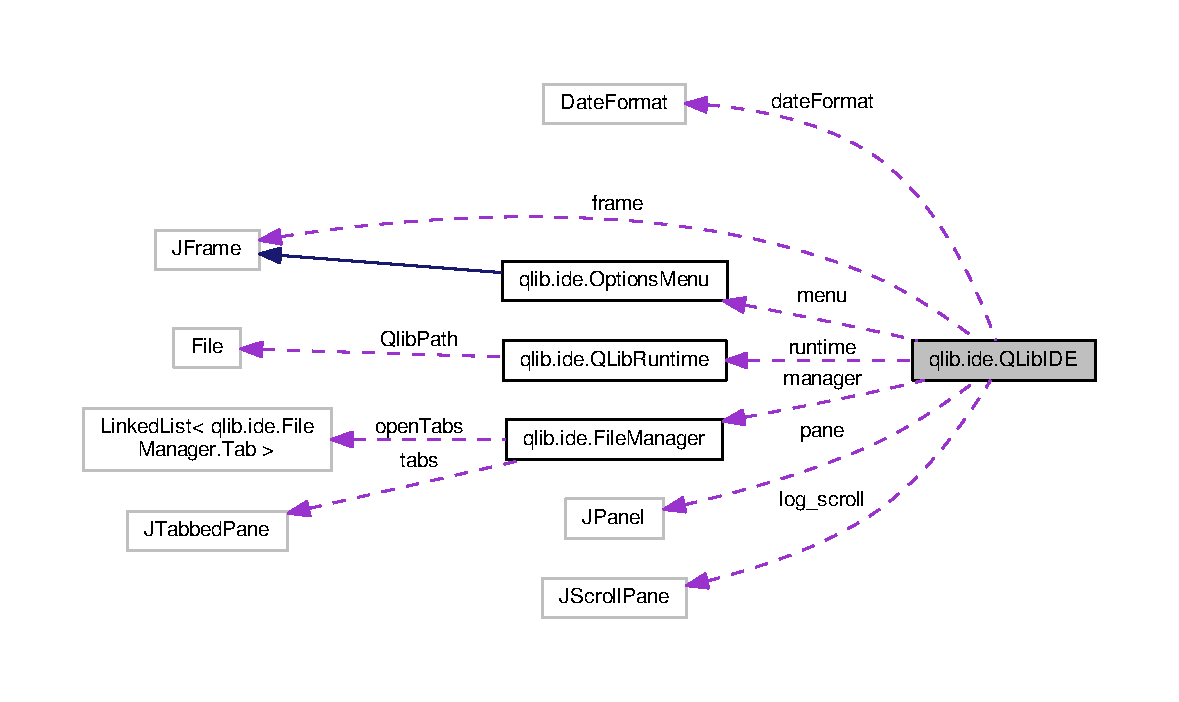
\includegraphics[width=350pt]{classqlib_1_1ide_1_1QLibIDE__coll__graph}
\end{center}
\end{figure}
\subsection*{Public Member Functions}
\begin{DoxyCompactItemize}
\item 
\hyperlink{classqlib_1_1ide_1_1QLibIDE_a3eafdf56320c066383975e5b2d22503a}{Q\+Lib\+I\+DE} (\hyperlink{classqlib_1_1ide_1_1IniIO}{Ini\+IO} config)  throws I\+O\+Exception
\item 
void \hyperlink{classqlib_1_1ide_1_1QLibIDE_aa0b95da9f912317b1497e190748733d6}{log} (Object message)
\item 
void \hyperlink{classqlib_1_1ide_1_1QLibIDE_a53bc0b691fd24d3e2dad2603cf086760}{show} ()
\end{DoxyCompactItemize}
\subsection*{Static Public Member Functions}
\begin{DoxyCompactItemize}
\item 
static void \hyperlink{classqlib_1_1ide_1_1QLibIDE_a4d8a71cb808c1796b48f83b05e3ca1b8}{main} (String\mbox{[}$\,$\mbox{]} args)
\end{DoxyCompactItemize}
\subsection*{Static Public Attributes}
\begin{DoxyCompactItemize}
\item 
static final String \hyperlink{classqlib_1_1ide_1_1QLibIDE_ae54da93b399d4d027f33c04ba7e392fd}{config\+Location} = \char`\"{}config.\+ini\char`\"{}
\item 
static final String \hyperlink{classqlib_1_1ide_1_1QLibIDE_aeaa0895eee29e9d5cf4e657134d56803}{online\+Resources} = \char`\"{}https\+://github.\+com/qkmaxware/Qlib\char`\"{}
\end{DoxyCompactItemize}
\subsection*{Private Member Functions}
\begin{DoxyCompactItemize}
\item 
void \hyperlink{classqlib_1_1ide_1_1QLibIDE_a6f9aa8bdf86b91b456239c96202d2e3f}{add\+Shortcut\+Key} (int key, Mouse\+Listener\mbox{[}$\,$\mbox{]} listeners)
\end{DoxyCompactItemize}
\subsection*{Private Attributes}
\begin{DoxyCompactItemize}
\item 
final J\+Frame \hyperlink{classqlib_1_1ide_1_1QLibIDE_a13a62cb428150031089c3824f16d6bef}{frame}
\item 
final J\+Panel \hyperlink{classqlib_1_1ide_1_1QLibIDE_a599d44725656f74ca6d6fc028b8973a8}{pane}
\item 
final J\+Text\+Area \hyperlink{classqlib_1_1ide_1_1QLibIDE_aa92d671c5f0158e59c86767109afc92c}{log}
\item 
final J\+Scroll\+Pane \hyperlink{classqlib_1_1ide_1_1QLibIDE_a74ee30733f7d424f2e518f1171d70917}{log\+\_\+scroll}
\item 
final \hyperlink{classqlib_1_1ide_1_1FileManager}{File\+Manager} \hyperlink{classqlib_1_1ide_1_1QLibIDE_a5af68fc042aeee1b69f27f3e1e67610b}{manager} = new \hyperlink{classqlib_1_1ide_1_1FileManager}{File\+Manager}()
\item 
\hyperlink{classqlib_1_1ide_1_1OptionsMenu}{Options\+Menu} \hyperlink{classqlib_1_1ide_1_1QLibIDE_ae822573114cbc618b4af0ddf3726b06b}{menu}
\item 
final Date\+Format \hyperlink{classqlib_1_1ide_1_1QLibIDE_ac1128e9b1f1d79af9c480383ab6a16ac}{date\+Format} = new Simple\+Date\+Format(\char`\"{}yyyy/MM/dd H\+H\+:mm\+:ss\char`\"{})
\item 
final \hyperlink{classqlib_1_1ide_1_1QLibRuntime}{Q\+Lib\+Runtime} \hyperlink{classqlib_1_1ide_1_1QLibIDE_a07b6d9558a76bd5d818a98debdb93d5f}{runtime}
\end{DoxyCompactItemize}


\subsection{Detailed Description}
Class for the Qlib\+I\+DE \begin{DoxyAuthor}{Author}
halse 
\end{DoxyAuthor}


\subsection{Constructor \& Destructor Documentation}
\index{qlib\+::ide\+::\+Q\+Lib\+I\+DE@{qlib\+::ide\+::\+Q\+Lib\+I\+DE}!Q\+Lib\+I\+DE@{Q\+Lib\+I\+DE}}
\index{Q\+Lib\+I\+DE@{Q\+Lib\+I\+DE}!qlib\+::ide\+::\+Q\+Lib\+I\+DE@{qlib\+::ide\+::\+Q\+Lib\+I\+DE}}
\subsubsection[{\texorpdfstring{Q\+Lib\+I\+D\+E(\+Ini\+I\+O config)}{QLibIDE(IniIO config)}}]{\setlength{\rightskip}{0pt plus 5cm}qlib.\+ide.\+Q\+Lib\+I\+D\+E.\+Q\+Lib\+I\+DE (
\begin{DoxyParamCaption}
\item[{{\bf Ini\+IO}}]{config}
\end{DoxyParamCaption}
) throws I\+O\+Exception\hspace{0.3cm}{\ttfamily [inline]}}\hypertarget{classqlib_1_1ide_1_1QLibIDE_a3eafdf56320c066383975e5b2d22503a}{}\label{classqlib_1_1ide_1_1QLibIDE_a3eafdf56320c066383975e5b2d22503a}
Create a new I\+DE instance 
\begin{DoxyParams}{Parameters}
{\em config} & \\
\hline
\end{DoxyParams}

\begin{DoxyExceptions}{Exceptions}
{\em I\+O\+Exception} & \\
\hline
\end{DoxyExceptions}


\subsection{Member Function Documentation}
\index{qlib\+::ide\+::\+Q\+Lib\+I\+DE@{qlib\+::ide\+::\+Q\+Lib\+I\+DE}!add\+Shortcut\+Key@{add\+Shortcut\+Key}}
\index{add\+Shortcut\+Key@{add\+Shortcut\+Key}!qlib\+::ide\+::\+Q\+Lib\+I\+DE@{qlib\+::ide\+::\+Q\+Lib\+I\+DE}}
\subsubsection[{\texorpdfstring{add\+Shortcut\+Key(int key, Mouse\+Listener[] listeners)}{addShortcutKey(int key, MouseListener[] listeners)}}]{\setlength{\rightskip}{0pt plus 5cm}void qlib.\+ide.\+Q\+Lib\+I\+D\+E.\+add\+Shortcut\+Key (
\begin{DoxyParamCaption}
\item[{int}]{key, }
\item[{Mouse\+Listener\mbox{[}$\,$\mbox{]}}]{listeners}
\end{DoxyParamCaption}
)\hspace{0.3cm}{\ttfamily [inline]}, {\ttfamily [private]}}\hypertarget{classqlib_1_1ide_1_1QLibIDE_a6f9aa8bdf86b91b456239c96202d2e3f}{}\label{classqlib_1_1ide_1_1QLibIDE_a6f9aa8bdf86b91b456239c96202d2e3f}
Add a key press shortcut to the I\+DE 
\begin{DoxyParams}{Parameters}
{\em key} & \\
\hline
{\em listeners} & \\
\hline
\end{DoxyParams}
\index{qlib\+::ide\+::\+Q\+Lib\+I\+DE@{qlib\+::ide\+::\+Q\+Lib\+I\+DE}!log@{log}}
\index{log@{log}!qlib\+::ide\+::\+Q\+Lib\+I\+DE@{qlib\+::ide\+::\+Q\+Lib\+I\+DE}}
\subsubsection[{\texorpdfstring{log(\+Object message)}{log(Object message)}}]{\setlength{\rightskip}{0pt plus 5cm}void qlib.\+ide.\+Q\+Lib\+I\+D\+E.\+log (
\begin{DoxyParamCaption}
\item[{Object}]{message}
\end{DoxyParamCaption}
)\hspace{0.3cm}{\ttfamily [inline]}}\hypertarget{classqlib_1_1ide_1_1QLibIDE_aa0b95da9f912317b1497e190748733d6}{}\label{classqlib_1_1ide_1_1QLibIDE_aa0b95da9f912317b1497e190748733d6}
Add a string to the log 
\begin{DoxyParams}{Parameters}
{\em message} & \\
\hline
\end{DoxyParams}
\index{qlib\+::ide\+::\+Q\+Lib\+I\+DE@{qlib\+::ide\+::\+Q\+Lib\+I\+DE}!main@{main}}
\index{main@{main}!qlib\+::ide\+::\+Q\+Lib\+I\+DE@{qlib\+::ide\+::\+Q\+Lib\+I\+DE}}
\subsubsection[{\texorpdfstring{main(\+String[] args)}{main(String[] args)}}]{\setlength{\rightskip}{0pt plus 5cm}static void qlib.\+ide.\+Q\+Lib\+I\+D\+E.\+main (
\begin{DoxyParamCaption}
\item[{String\mbox{[}$\,$\mbox{]}}]{args}
\end{DoxyParamCaption}
)\hspace{0.3cm}{\ttfamily [inline]}, {\ttfamily [static]}}\hypertarget{classqlib_1_1ide_1_1QLibIDE_a4d8a71cb808c1796b48f83b05e3ca1b8}{}\label{classqlib_1_1ide_1_1QLibIDE_a4d8a71cb808c1796b48f83b05e3ca1b8}

\begin{DoxyParams}{Parameters}
{\em args} & the command line arguments \\
\hline
\end{DoxyParams}
\index{qlib\+::ide\+::\+Q\+Lib\+I\+DE@{qlib\+::ide\+::\+Q\+Lib\+I\+DE}!show@{show}}
\index{show@{show}!qlib\+::ide\+::\+Q\+Lib\+I\+DE@{qlib\+::ide\+::\+Q\+Lib\+I\+DE}}
\subsubsection[{\texorpdfstring{show()}{show()}}]{\setlength{\rightskip}{0pt plus 5cm}void qlib.\+ide.\+Q\+Lib\+I\+D\+E.\+show (
\begin{DoxyParamCaption}
{}
\end{DoxyParamCaption}
)\hspace{0.3cm}{\ttfamily [inline]}}\hypertarget{classqlib_1_1ide_1_1QLibIDE_a53bc0b691fd24d3e2dad2603cf086760}{}\label{classqlib_1_1ide_1_1QLibIDE_a53bc0b691fd24d3e2dad2603cf086760}
Show the I\+DE 

\subsection{Member Data Documentation}
\index{qlib\+::ide\+::\+Q\+Lib\+I\+DE@{qlib\+::ide\+::\+Q\+Lib\+I\+DE}!config\+Location@{config\+Location}}
\index{config\+Location@{config\+Location}!qlib\+::ide\+::\+Q\+Lib\+I\+DE@{qlib\+::ide\+::\+Q\+Lib\+I\+DE}}
\subsubsection[{\texorpdfstring{config\+Location}{configLocation}}]{\setlength{\rightskip}{0pt plus 5cm}final String qlib.\+ide.\+Q\+Lib\+I\+D\+E.\+config\+Location = \char`\"{}config.\+ini\char`\"{}\hspace{0.3cm}{\ttfamily [static]}}\hypertarget{classqlib_1_1ide_1_1QLibIDE_ae54da93b399d4d027f33c04ba7e392fd}{}\label{classqlib_1_1ide_1_1QLibIDE_ae54da93b399d4d027f33c04ba7e392fd}
Location of the config file \index{qlib\+::ide\+::\+Q\+Lib\+I\+DE@{qlib\+::ide\+::\+Q\+Lib\+I\+DE}!date\+Format@{date\+Format}}
\index{date\+Format@{date\+Format}!qlib\+::ide\+::\+Q\+Lib\+I\+DE@{qlib\+::ide\+::\+Q\+Lib\+I\+DE}}
\subsubsection[{\texorpdfstring{date\+Format}{dateFormat}}]{\setlength{\rightskip}{0pt plus 5cm}final Date\+Format qlib.\+ide.\+Q\+Lib\+I\+D\+E.\+date\+Format = new Simple\+Date\+Format(\char`\"{}yyyy/MM/dd H\+H\+:mm\+:ss\char`\"{})\hspace{0.3cm}{\ttfamily [private]}}\hypertarget{classqlib_1_1ide_1_1QLibIDE_ac1128e9b1f1d79af9c480383ab6a16ac}{}\label{classqlib_1_1ide_1_1QLibIDE_ac1128e9b1f1d79af9c480383ab6a16ac}
Date format \index{qlib\+::ide\+::\+Q\+Lib\+I\+DE@{qlib\+::ide\+::\+Q\+Lib\+I\+DE}!frame@{frame}}
\index{frame@{frame}!qlib\+::ide\+::\+Q\+Lib\+I\+DE@{qlib\+::ide\+::\+Q\+Lib\+I\+DE}}
\subsubsection[{\texorpdfstring{frame}{frame}}]{\setlength{\rightskip}{0pt plus 5cm}final J\+Frame qlib.\+ide.\+Q\+Lib\+I\+D\+E.\+frame\hspace{0.3cm}{\ttfamily [private]}}\hypertarget{classqlib_1_1ide_1_1QLibIDE_a13a62cb428150031089c3824f16d6bef}{}\label{classqlib_1_1ide_1_1QLibIDE_a13a62cb428150031089c3824f16d6bef}
Reference to the frame \index{qlib\+::ide\+::\+Q\+Lib\+I\+DE@{qlib\+::ide\+::\+Q\+Lib\+I\+DE}!log@{log}}
\index{log@{log}!qlib\+::ide\+::\+Q\+Lib\+I\+DE@{qlib\+::ide\+::\+Q\+Lib\+I\+DE}}
\subsubsection[{\texorpdfstring{log}{log}}]{\setlength{\rightskip}{0pt plus 5cm}final J\+Text\+Area qlib.\+ide.\+Q\+Lib\+I\+D\+E.\+log\hspace{0.3cm}{\ttfamily [private]}}\hypertarget{classqlib_1_1ide_1_1QLibIDE_aa92d671c5f0158e59c86767109afc92c}{}\label{classqlib_1_1ide_1_1QLibIDE_aa92d671c5f0158e59c86767109afc92c}
Reference to the output log \index{qlib\+::ide\+::\+Q\+Lib\+I\+DE@{qlib\+::ide\+::\+Q\+Lib\+I\+DE}!log\+\_\+scroll@{log\+\_\+scroll}}
\index{log\+\_\+scroll@{log\+\_\+scroll}!qlib\+::ide\+::\+Q\+Lib\+I\+DE@{qlib\+::ide\+::\+Q\+Lib\+I\+DE}}
\subsubsection[{\texorpdfstring{log\+\_\+scroll}{log_scroll}}]{\setlength{\rightskip}{0pt plus 5cm}final J\+Scroll\+Pane qlib.\+ide.\+Q\+Lib\+I\+D\+E.\+log\+\_\+scroll\hspace{0.3cm}{\ttfamily [private]}}\hypertarget{classqlib_1_1ide_1_1QLibIDE_a74ee30733f7d424f2e518f1171d70917}{}\label{classqlib_1_1ide_1_1QLibIDE_a74ee30733f7d424f2e518f1171d70917}
Reference to the scroll panel for the output log \index{qlib\+::ide\+::\+Q\+Lib\+I\+DE@{qlib\+::ide\+::\+Q\+Lib\+I\+DE}!manager@{manager}}
\index{manager@{manager}!qlib\+::ide\+::\+Q\+Lib\+I\+DE@{qlib\+::ide\+::\+Q\+Lib\+I\+DE}}
\subsubsection[{\texorpdfstring{manager}{manager}}]{\setlength{\rightskip}{0pt plus 5cm}final {\bf File\+Manager} qlib.\+ide.\+Q\+Lib\+I\+D\+E.\+manager = new {\bf File\+Manager}()\hspace{0.3cm}{\ttfamily [private]}}\hypertarget{classqlib_1_1ide_1_1QLibIDE_a5af68fc042aeee1b69f27f3e1e67610b}{}\label{classqlib_1_1ide_1_1QLibIDE_a5af68fc042aeee1b69f27f3e1e67610b}
Reference to the tabbed pane for file managers \index{qlib\+::ide\+::\+Q\+Lib\+I\+DE@{qlib\+::ide\+::\+Q\+Lib\+I\+DE}!menu@{menu}}
\index{menu@{menu}!qlib\+::ide\+::\+Q\+Lib\+I\+DE@{qlib\+::ide\+::\+Q\+Lib\+I\+DE}}
\subsubsection[{\texorpdfstring{menu}{menu}}]{\setlength{\rightskip}{0pt plus 5cm}{\bf Options\+Menu} qlib.\+ide.\+Q\+Lib\+I\+D\+E.\+menu\hspace{0.3cm}{\ttfamily [private]}}\hypertarget{classqlib_1_1ide_1_1QLibIDE_ae822573114cbc618b4af0ddf3726b06b}{}\label{classqlib_1_1ide_1_1QLibIDE_ae822573114cbc618b4af0ddf3726b06b}
UI for configuring options \index{qlib\+::ide\+::\+Q\+Lib\+I\+DE@{qlib\+::ide\+::\+Q\+Lib\+I\+DE}!online\+Resources@{online\+Resources}}
\index{online\+Resources@{online\+Resources}!qlib\+::ide\+::\+Q\+Lib\+I\+DE@{qlib\+::ide\+::\+Q\+Lib\+I\+DE}}
\subsubsection[{\texorpdfstring{online\+Resources}{onlineResources}}]{\setlength{\rightskip}{0pt plus 5cm}final String qlib.\+ide.\+Q\+Lib\+I\+D\+E.\+online\+Resources = \char`\"{}https\+://github.\+com/qkmaxware/Qlib\char`\"{}\hspace{0.3cm}{\ttfamily [static]}}\hypertarget{classqlib_1_1ide_1_1QLibIDE_aeaa0895eee29e9d5cf4e657134d56803}{}\label{classqlib_1_1ide_1_1QLibIDE_aeaa0895eee29e9d5cf4e657134d56803}
Location to the online resources for Qlib \index{qlib\+::ide\+::\+Q\+Lib\+I\+DE@{qlib\+::ide\+::\+Q\+Lib\+I\+DE}!pane@{pane}}
\index{pane@{pane}!qlib\+::ide\+::\+Q\+Lib\+I\+DE@{qlib\+::ide\+::\+Q\+Lib\+I\+DE}}
\subsubsection[{\texorpdfstring{pane}{pane}}]{\setlength{\rightskip}{0pt plus 5cm}final J\+Panel qlib.\+ide.\+Q\+Lib\+I\+D\+E.\+pane\hspace{0.3cm}{\ttfamily [private]}}\hypertarget{classqlib_1_1ide_1_1QLibIDE_a599d44725656f74ca6d6fc028b8973a8}{}\label{classqlib_1_1ide_1_1QLibIDE_a599d44725656f74ca6d6fc028b8973a8}
Reference to the central panel \index{qlib\+::ide\+::\+Q\+Lib\+I\+DE@{qlib\+::ide\+::\+Q\+Lib\+I\+DE}!runtime@{runtime}}
\index{runtime@{runtime}!qlib\+::ide\+::\+Q\+Lib\+I\+DE@{qlib\+::ide\+::\+Q\+Lib\+I\+DE}}
\subsubsection[{\texorpdfstring{runtime}{runtime}}]{\setlength{\rightskip}{0pt plus 5cm}final {\bf Q\+Lib\+Runtime} qlib.\+ide.\+Q\+Lib\+I\+D\+E.\+runtime\hspace{0.3cm}{\ttfamily [private]}}\hypertarget{classqlib_1_1ide_1_1QLibIDE_a07b6d9558a76bd5d818a98debdb93d5f}{}\label{classqlib_1_1ide_1_1QLibIDE_a07b6d9558a76bd5d818a98debdb93d5f}
Reference to class for executing the Q\+Lib runtime 

The documentation for this class was generated from the following file\+:\begin{DoxyCompactItemize}
\item 
src/ide/src/qlib/ide/\hyperlink{QLibIDE_8java}{Q\+Lib\+I\+D\+E.\+java}\end{DoxyCompactItemize}

\hypertarget{classqlib_1_1ide_1_1QLibRuntime}{}\section{qlib.\+ide.\+Q\+Lib\+Runtime Class Reference}
\label{classqlib_1_1ide_1_1QLibRuntime}\index{qlib.\+ide.\+Q\+Lib\+Runtime@{qlib.\+ide.\+Q\+Lib\+Runtime}}


Collaboration diagram for qlib.\+ide.\+Q\+Lib\+Runtime\+:\nopagebreak
\begin{figure}[H]
\begin{center}
\leavevmode
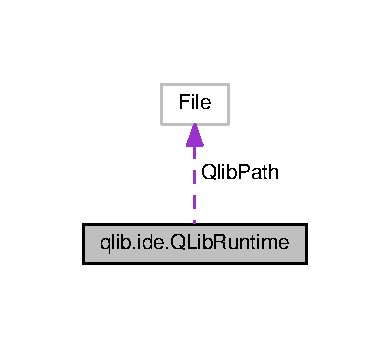
\includegraphics[width=187pt]{classqlib_1_1ide_1_1QLibRuntime__coll__graph}
\end{center}
\end{figure}
\subsection*{Public Member Functions}
\begin{DoxyCompactItemize}
\item 
\hyperlink{classqlib_1_1ide_1_1QLibRuntime_a8525f2178485c12a94d9caf9fb09d47c}{Q\+Lib\+Runtime} (File \hyperlink{classqlib_1_1ide_1_1QLibRuntime_a4f27be4c59b8b5005822acc9e36e1279}{Qlib\+Path})
\item 
\hyperlink{classqlib_1_1ide_1_1RuntimeReport}{Runtime\+Report} \hyperlink{classqlib_1_1ide_1_1QLibRuntime_a6e2d353e7b2bcd11ac50ee0e6465f044}{dispatch} (File f)  throws I\+O\+Exception
\end{DoxyCompactItemize}
\subsection*{Private Attributes}
\begin{DoxyCompactItemize}
\item 
File \hyperlink{classqlib_1_1ide_1_1QLibRuntime_a4f27be4c59b8b5005822acc9e36e1279}{Qlib\+Path}
\end{DoxyCompactItemize}


\subsection{Detailed Description}
Class for sending files to the Q\+Lib runtime executable \begin{DoxyAuthor}{Author}
halse 
\end{DoxyAuthor}


\subsection{Constructor \& Destructor Documentation}
\index{qlib\+::ide\+::\+Q\+Lib\+Runtime@{qlib\+::ide\+::\+Q\+Lib\+Runtime}!Q\+Lib\+Runtime@{Q\+Lib\+Runtime}}
\index{Q\+Lib\+Runtime@{Q\+Lib\+Runtime}!qlib\+::ide\+::\+Q\+Lib\+Runtime@{qlib\+::ide\+::\+Q\+Lib\+Runtime}}
\subsubsection[{\texorpdfstring{Q\+Lib\+Runtime(\+File Qlib\+Path)}{QLibRuntime(File QlibPath)}}]{\setlength{\rightskip}{0pt plus 5cm}qlib.\+ide.\+Q\+Lib\+Runtime.\+Q\+Lib\+Runtime (
\begin{DoxyParamCaption}
\item[{File}]{Qlib\+Path}
\end{DoxyParamCaption}
)\hspace{0.3cm}{\ttfamily [inline]}}\hypertarget{classqlib_1_1ide_1_1QLibRuntime_a8525f2178485c12a94d9caf9fb09d47c}{}\label{classqlib_1_1ide_1_1QLibRuntime_a8525f2178485c12a94d9caf9fb09d47c}
Create a Qlib runtime reference to the given file 
\begin{DoxyParams}{Parameters}
{\em Qlib\+Path} & \\
\hline
\end{DoxyParams}


\subsection{Member Function Documentation}
\index{qlib\+::ide\+::\+Q\+Lib\+Runtime@{qlib\+::ide\+::\+Q\+Lib\+Runtime}!dispatch@{dispatch}}
\index{dispatch@{dispatch}!qlib\+::ide\+::\+Q\+Lib\+Runtime@{qlib\+::ide\+::\+Q\+Lib\+Runtime}}
\subsubsection[{\texorpdfstring{dispatch(\+File f)}{dispatch(File f)}}]{\setlength{\rightskip}{0pt plus 5cm}{\bf Runtime\+Report} qlib.\+ide.\+Q\+Lib\+Runtime.\+dispatch (
\begin{DoxyParamCaption}
\item[{File}]{f}
\end{DoxyParamCaption}
) throws I\+O\+Exception\hspace{0.3cm}{\ttfamily [inline]}}\hypertarget{classqlib_1_1ide_1_1QLibRuntime_a6e2d353e7b2bcd11ac50ee0e6465f044}{}\label{classqlib_1_1ide_1_1QLibRuntime_a6e2d353e7b2bcd11ac50ee0e6465f044}
Invoke the Q\+Lib runtime and pass in the given file 
\begin{DoxyParams}{Parameters}
{\em f} & \\
\hline
\end{DoxyParams}
\begin{DoxyReturn}{Returns}

\end{DoxyReturn}

\begin{DoxyExceptions}{Exceptions}
{\em I\+O\+Exception} & \\
\hline
\end{DoxyExceptions}


\subsection{Member Data Documentation}
\index{qlib\+::ide\+::\+Q\+Lib\+Runtime@{qlib\+::ide\+::\+Q\+Lib\+Runtime}!Qlib\+Path@{Qlib\+Path}}
\index{Qlib\+Path@{Qlib\+Path}!qlib\+::ide\+::\+Q\+Lib\+Runtime@{qlib\+::ide\+::\+Q\+Lib\+Runtime}}
\subsubsection[{\texorpdfstring{Qlib\+Path}{QlibPath}}]{\setlength{\rightskip}{0pt plus 5cm}File qlib.\+ide.\+Q\+Lib\+Runtime.\+Qlib\+Path\hspace{0.3cm}{\ttfamily [private]}}\hypertarget{classqlib_1_1ide_1_1QLibRuntime_a4f27be4c59b8b5005822acc9e36e1279}{}\label{classqlib_1_1ide_1_1QLibRuntime_a4f27be4c59b8b5005822acc9e36e1279}
Reference to the Q\+Lib runtime file 

The documentation for this class was generated from the following file\+:\begin{DoxyCompactItemize}
\item 
src/ide/src/qlib/ide/\hyperlink{QLibRuntime_8java}{Q\+Lib\+Runtime.\+java}\end{DoxyCompactItemize}

\hypertarget{classqlib_1_1quantum_1_1qreg}{}\section{qlib\+:\+:quantum\+:\+:qreg Class Reference}
\label{classqlib_1_1quantum_1_1qreg}\index{qlib\+::quantum\+::qreg@{qlib\+::quantum\+::qreg}}


{\ttfamily \#include $<$qreg.\+hpp$>$}



Inheritance diagram for qlib\+:\+:quantum\+:\+:qreg\+:\nopagebreak
\begin{figure}[H]
\begin{center}
\leavevmode
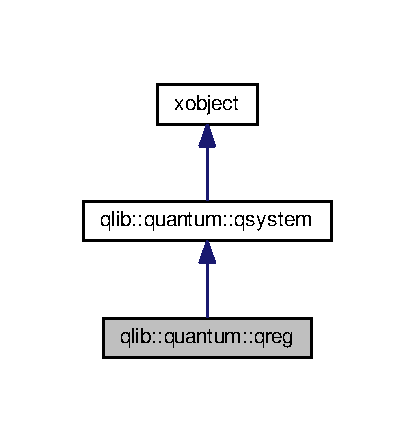
\includegraphics[width=199pt]{classqlib_1_1quantum_1_1qreg__inherit__graph}
\end{center}
\end{figure}


Collaboration diagram for qlib\+:\+:quantum\+:\+:qreg\+:\nopagebreak
\begin{figure}[H]
\begin{center}
\leavevmode
\includegraphics[width=310pt]{classqlib_1_1quantum_1_1qreg__coll__graph}
\end{center}
\end{figure}
\subsection*{Public Member Functions}
\begin{DoxyCompactItemize}
\item 
\hyperlink{classqlib_1_1quantum_1_1qreg_aa53d83236917f0048965b487088aacb9}{qreg} ()
\item 
\hyperlink{classqlib_1_1quantum_1_1qreg_a2ddfaef9a369571c9600c4c259fcb8b1}{qreg} (u32 \hyperlink{classqlib_1_1quantum_1_1qreg_a2d7c33e71a77d860d50d53a258a71a6f}{qubits})
\item 
size\+\_\+t \hyperlink{classqlib_1_1quantum_1_1qreg_a3148742b59865d0ba04fdd327fccc048}{size} ()
\item 
\hyperlink{classqlib_1_1math_1_1matrix}{matrix} \& \hyperlink{classqlib_1_1quantum_1_1qreg_a20d1b0906eb00ff7d4e1c23449de61a1}{state} ()
\item 
void \hyperlink{classqlib_1_1quantum_1_1qreg_af38f95ecaaf7de400856094154343cfe}{apply} (\hyperlink{classqlib_1_1quantum_1_1gates_1_1igate}{qlib\+::quantum\+::gates\+::igate} \&gate, std\+::vector$<$ u64 $>$ input\+Bits)
\item 
i8 \hyperlink{classqlib_1_1quantum_1_1qreg_acfcd58502c1e511766ede52a891f27c3}{measure} (i64 \hyperlink{classqlib_1_1quantum_1_1qubit}{qubit})
\item 
virtual void \hyperlink{classqlib_1_1quantum_1_1qreg_a51eb9abfde64d764ca2afa27666df0e1}{zero} (i64 \hyperlink{classqlib_1_1quantum_1_1qubit}{qubit})
\item 
std\+::string \hyperlink{classqlib_1_1quantum_1_1qreg_ae4dbf316bf6452f3110cb05146f54954}{to\+String} ()
\end{DoxyCompactItemize}
\subsection*{Private Attributes}
\begin{DoxyCompactItemize}
\item 
u32 \hyperlink{classqlib_1_1quantum_1_1qreg_a2d7c33e71a77d860d50d53a258a71a6f}{qubits}
\item 
u32 \hyperlink{classqlib_1_1quantum_1_1qreg_ad0e84b959f93f3da6ed81eb096f809d1}{states}
\item 
\hyperlink{classqlib_1_1math_1_1matrix}{matrix} \hyperlink{classqlib_1_1quantum_1_1qreg_a1a7e244ee72b78b9c5a8763efad57ada}{amplitudes}
\item 
std\+::uniform\+\_\+real\+\_\+distribution$<$ f32 $>$ \hyperlink{classqlib_1_1quantum_1_1qreg_aabd605497170f57cdbb175d21c99662e}{distribution}
\end{DoxyCompactItemize}


\subsection{Detailed Description}
Represents a register of \textquotesingle{}N\textquotesingle{} qubits 

\subsection{Constructor \& Destructor Documentation}
\index{qlib\+::quantum\+::qreg@{qlib\+::quantum\+::qreg}!qreg@{qreg}}
\index{qreg@{qreg}!qlib\+::quantum\+::qreg@{qlib\+::quantum\+::qreg}}
\subsubsection[{\texorpdfstring{qreg()}{qreg()}}]{\setlength{\rightskip}{0pt plus 5cm}qlib\+::quantum\+::qreg\+::qreg (
\begin{DoxyParamCaption}
{}
\end{DoxyParamCaption}
)\hspace{0.3cm}{\ttfamily [inline]}}\hypertarget{classqlib_1_1quantum_1_1qreg_aa53d83236917f0048965b487088aacb9}{}\label{classqlib_1_1quantum_1_1qreg_aa53d83236917f0048965b487088aacb9}
Quantum register of 1 qubit \index{qlib\+::quantum\+::qreg@{qlib\+::quantum\+::qreg}!qreg@{qreg}}
\index{qreg@{qreg}!qlib\+::quantum\+::qreg@{qlib\+::quantum\+::qreg}}
\subsubsection[{\texorpdfstring{qreg(u32 qubits)}{qreg(u32 qubits)}}]{\setlength{\rightskip}{0pt plus 5cm}qlib\+::quantum\+::qreg\+::qreg (
\begin{DoxyParamCaption}
\item[{u32}]{qubits}
\end{DoxyParamCaption}
)\hspace{0.3cm}{\ttfamily [inline]}}\hypertarget{classqlib_1_1quantum_1_1qreg_a2ddfaef9a369571c9600c4c259fcb8b1}{}\label{classqlib_1_1quantum_1_1qreg_a2ddfaef9a369571c9600c4c259fcb8b1}
Quantum register of \textquotesingle{}N\textquotesingle{} qubits 

\subsection{Member Function Documentation}
\index{qlib\+::quantum\+::qreg@{qlib\+::quantum\+::qreg}!apply@{apply}}
\index{apply@{apply}!qlib\+::quantum\+::qreg@{qlib\+::quantum\+::qreg}}
\subsubsection[{\texorpdfstring{apply(qlib\+::quantum\+::gates\+::igate \&gate, std\+::vector$<$ u64 $>$ input\+Bits)}{apply(qlib::quantum::gates::igate &gate, std::vector< u64 > inputBits)}}]{\setlength{\rightskip}{0pt plus 5cm}void qlib\+::quantum\+::qreg\+::apply (
\begin{DoxyParamCaption}
\item[{{\bf qlib\+::quantum\+::gates\+::igate} \&}]{gate, }
\item[{std\+::vector$<$ u64 $>$}]{input\+Bits}
\end{DoxyParamCaption}
)\hspace{0.3cm}{\ttfamily [inline]}, {\ttfamily [virtual]}}\hypertarget{classqlib_1_1quantum_1_1qreg_af38f95ecaaf7de400856094154343cfe}{}\label{classqlib_1_1quantum_1_1qreg_af38f95ecaaf7de400856094154343cfe}
Apply a quantum gate to this system 

Implements \hyperlink{classqlib_1_1quantum_1_1qsystem_adbb748feb351aac69ca4a0bf6c92d77c}{qlib\+::quantum\+::qsystem}.

\index{qlib\+::quantum\+::qreg@{qlib\+::quantum\+::qreg}!measure@{measure}}
\index{measure@{measure}!qlib\+::quantum\+::qreg@{qlib\+::quantum\+::qreg}}
\subsubsection[{\texorpdfstring{measure(i64 qubit)}{measure(i64 qubit)}}]{\setlength{\rightskip}{0pt plus 5cm}i8 qlib\+::quantum\+::qreg\+::measure (
\begin{DoxyParamCaption}
\item[{i64}]{qubit}
\end{DoxyParamCaption}
)\hspace{0.3cm}{\ttfamily [inline]}, {\ttfamily [virtual]}}\hypertarget{classqlib_1_1quantum_1_1qreg_acfcd58502c1e511766ede52a891f27c3}{}\label{classqlib_1_1quantum_1_1qreg_acfcd58502c1e511766ede52a891f27c3}
Collapse the state and return the value of the measured qubit 

Implements \hyperlink{classqlib_1_1quantum_1_1qsystem_a33d9954c6ca01cb400d940ff05614364}{qlib\+::quantum\+::qsystem}.

\index{qlib\+::quantum\+::qreg@{qlib\+::quantum\+::qreg}!size@{size}}
\index{size@{size}!qlib\+::quantum\+::qreg@{qlib\+::quantum\+::qreg}}
\subsubsection[{\texorpdfstring{size()}{size()}}]{\setlength{\rightskip}{0pt plus 5cm}size\+\_\+t qlib\+::quantum\+::qreg\+::size (
\begin{DoxyParamCaption}
{}
\end{DoxyParamCaption}
)\hspace{0.3cm}{\ttfamily [inline]}}\hypertarget{classqlib_1_1quantum_1_1qreg_a3148742b59865d0ba04fdd327fccc048}{}\label{classqlib_1_1quantum_1_1qreg_a3148742b59865d0ba04fdd327fccc048}
Number of qubits in this register \index{qlib\+::quantum\+::qreg@{qlib\+::quantum\+::qreg}!state@{state}}
\index{state@{state}!qlib\+::quantum\+::qreg@{qlib\+::quantum\+::qreg}}
\subsubsection[{\texorpdfstring{state()}{state()}}]{\setlength{\rightskip}{0pt plus 5cm}{\bf matrix}\& qlib\+::quantum\+::qreg\+::state (
\begin{DoxyParamCaption}
{}
\end{DoxyParamCaption}
)\hspace{0.3cm}{\ttfamily [inline]}}\hypertarget{classqlib_1_1quantum_1_1qreg_a20d1b0906eb00ff7d4e1c23449de61a1}{}\label{classqlib_1_1quantum_1_1qreg_a20d1b0906eb00ff7d4e1c23449de61a1}
Get the complex amplitude matrix \index{qlib\+::quantum\+::qreg@{qlib\+::quantum\+::qreg}!to\+String@{to\+String}}
\index{to\+String@{to\+String}!qlib\+::quantum\+::qreg@{qlib\+::quantum\+::qreg}}
\subsubsection[{\texorpdfstring{to\+String()}{toString()}}]{\setlength{\rightskip}{0pt plus 5cm}std\+::string qlib\+::quantum\+::qreg\+::to\+String (
\begin{DoxyParamCaption}
{}
\end{DoxyParamCaption}
)\hspace{0.3cm}{\ttfamily [inline]}, {\ttfamily [virtual]}}\hypertarget{classqlib_1_1quantum_1_1qreg_ae4dbf316bf6452f3110cb05146f54954}{}\label{classqlib_1_1quantum_1_1qreg_ae4dbf316bf6452f3110cb05146f54954}
Human readable output 

Reimplemented from \hyperlink{classqlib_1_1quantum_1_1qsystem_a9d95030955e2fdb26bc9152c32310e7e}{qlib\+::quantum\+::qsystem}.

\index{qlib\+::quantum\+::qreg@{qlib\+::quantum\+::qreg}!zero@{zero}}
\index{zero@{zero}!qlib\+::quantum\+::qreg@{qlib\+::quantum\+::qreg}}
\subsubsection[{\texorpdfstring{zero(i64 qubit)}{zero(i64 qubit)}}]{\setlength{\rightskip}{0pt plus 5cm}virtual void qlib\+::quantum\+::qreg\+::zero (
\begin{DoxyParamCaption}
\item[{i64}]{qubit}
\end{DoxyParamCaption}
)\hspace{0.3cm}{\ttfamily [inline]}, {\ttfamily [virtual]}}\hypertarget{classqlib_1_1quantum_1_1qreg_a51eb9abfde64d764ca2afa27666df0e1}{}\label{classqlib_1_1quantum_1_1qreg_a51eb9abfde64d764ca2afa27666df0e1}
Prepare qubit in the zero state 

Implements \hyperlink{classqlib_1_1quantum_1_1qsystem_a5626857e5dc87dc2bdbb1f4d0b0401f9}{qlib\+::quantum\+::qsystem}.



\subsection{Member Data Documentation}
\index{qlib\+::quantum\+::qreg@{qlib\+::quantum\+::qreg}!amplitudes@{amplitudes}}
\index{amplitudes@{amplitudes}!qlib\+::quantum\+::qreg@{qlib\+::quantum\+::qreg}}
\subsubsection[{\texorpdfstring{amplitudes}{amplitudes}}]{\setlength{\rightskip}{0pt plus 5cm}{\bf matrix} qlib\+::quantum\+::qreg\+::amplitudes\hspace{0.3cm}{\ttfamily [private]}}\hypertarget{classqlib_1_1quantum_1_1qreg_a1a7e244ee72b78b9c5a8763efad57ada}{}\label{classqlib_1_1quantum_1_1qreg_a1a7e244ee72b78b9c5a8763efad57ada}
State vector of complex amplitudes \index{qlib\+::quantum\+::qreg@{qlib\+::quantum\+::qreg}!distribution@{distribution}}
\index{distribution@{distribution}!qlib\+::quantum\+::qreg@{qlib\+::quantum\+::qreg}}
\subsubsection[{\texorpdfstring{distribution}{distribution}}]{\setlength{\rightskip}{0pt plus 5cm}std\+::uniform\+\_\+real\+\_\+distribution$<$f32$>$ qlib\+::quantum\+::qreg\+::distribution\hspace{0.3cm}{\ttfamily [private]}}\hypertarget{classqlib_1_1quantum_1_1qreg_aabd605497170f57cdbb175d21c99662e}{}\label{classqlib_1_1quantum_1_1qreg_aabd605497170f57cdbb175d21c99662e}
Random distribution used during measurement \index{qlib\+::quantum\+::qreg@{qlib\+::quantum\+::qreg}!qubits@{qubits}}
\index{qubits@{qubits}!qlib\+::quantum\+::qreg@{qlib\+::quantum\+::qreg}}
\subsubsection[{\texorpdfstring{qubits}{qubits}}]{\setlength{\rightskip}{0pt plus 5cm}u32 qlib\+::quantum\+::qreg\+::qubits\hspace{0.3cm}{\ttfamily [private]}}\hypertarget{classqlib_1_1quantum_1_1qreg_a2d7c33e71a77d860d50d53a258a71a6f}{}\label{classqlib_1_1quantum_1_1qreg_a2d7c33e71a77d860d50d53a258a71a6f}
Number of qubits in this register \index{qlib\+::quantum\+::qreg@{qlib\+::quantum\+::qreg}!states@{states}}
\index{states@{states}!qlib\+::quantum\+::qreg@{qlib\+::quantum\+::qreg}}
\subsubsection[{\texorpdfstring{states}{states}}]{\setlength{\rightskip}{0pt plus 5cm}u32 qlib\+::quantum\+::qreg\+::states\hspace{0.3cm}{\ttfamily [private]}}\hypertarget{classqlib_1_1quantum_1_1qreg_ad0e84b959f93f3da6ed81eb096f809d1}{}\label{classqlib_1_1quantum_1_1qreg_ad0e84b959f93f3da6ed81eb096f809d1}
Number of states represented by the given number of qubits 

The documentation for this class was generated from the following file\+:\begin{DoxyCompactItemize}
\item 
src/core/quantum/systems/\hyperlink{qreg_8hpp}{qreg.\+hpp}\end{DoxyCompactItemize}

\hypertarget{classqlib_1_1quantum_1_1qsystem}{}\section{qlib\+:\+:quantum\+:\+:qsystem Class Reference}
\label{classqlib_1_1quantum_1_1qsystem}\index{qlib\+::quantum\+::qsystem@{qlib\+::quantum\+::qsystem}}


{\ttfamily \#include $<$system.\+hpp$>$}



Inheritance diagram for qlib\+:\+:quantum\+:\+:qsystem\+:\nopagebreak
\begin{figure}[H]
\begin{center}
\leavevmode
\includegraphics[width=350pt]{classqlib_1_1quantum_1_1qsystem__inherit__graph}
\end{center}
\end{figure}


Collaboration diagram for qlib\+:\+:quantum\+:\+:qsystem\+:\nopagebreak
\begin{figure}[H]
\begin{center}
\leavevmode
\includegraphics[width=199pt]{classqlib_1_1quantum_1_1qsystem__coll__graph}
\end{center}
\end{figure}
\subsection*{Public Member Functions}
\begin{DoxyCompactItemize}
\item 
virtual \hyperlink{classqlib_1_1quantum_1_1qsystem_aeb1ecc3086cd9c14756aa4c575eeda0c}{$\sim$qsystem} ()
\item 
virtual void \hyperlink{classqlib_1_1quantum_1_1qsystem_adbb748feb351aac69ca4a0bf6c92d77c}{apply} (\hyperlink{classqlib_1_1quantum_1_1gates_1_1igate}{qlib\+::quantum\+::gates\+::igate} \&gate, std\+::vector$<$ u64 $>$ input\+Bits)=0
\item 
virtual i8 \hyperlink{classqlib_1_1quantum_1_1qsystem_a33d9954c6ca01cb400d940ff05614364}{measure} (i64 \hyperlink{classqlib_1_1quantum_1_1qubit}{qubit})=0
\item 
virtual void \hyperlink{classqlib_1_1quantum_1_1qsystem_ab70360fa1be7b72d4f49f6dadc17267d}{set\+State} (std\+::vector$<$ \hyperlink{classqlib_1_1math_1_1complex}{complex} $>$ amp)=0
\item 
virtual std\+::string \hyperlink{classqlib_1_1quantum_1_1qsystem_a9d95030955e2fdb26bc9152c32310e7e}{to\+String} ()
\item 
virtual void \hyperlink{classqlib_1_1quantum_1_1qsystem_a5626857e5dc87dc2bdbb1f4d0b0401f9}{zero} (i64 \hyperlink{classqlib_1_1quantum_1_1qubit}{qubit})=0
\end{DoxyCompactItemize}


\subsection{Detailed Description}
Base class for all quantum systems 

\subsection{Constructor \& Destructor Documentation}
\index{qlib\+::quantum\+::qsystem@{qlib\+::quantum\+::qsystem}!````~qsystem@{$\sim$qsystem}}
\index{````~qsystem@{$\sim$qsystem}!qlib\+::quantum\+::qsystem@{qlib\+::quantum\+::qsystem}}
\subsubsection[{\texorpdfstring{$\sim$qsystem()}{~qsystem()}}]{\setlength{\rightskip}{0pt plus 5cm}virtual qlib\+::quantum\+::qsystem\+::$\sim$qsystem (
\begin{DoxyParamCaption}
{}
\end{DoxyParamCaption}
)\hspace{0.3cm}{\ttfamily [inline]}, {\ttfamily [virtual]}}\hypertarget{classqlib_1_1quantum_1_1qsystem_aeb1ecc3086cd9c14756aa4c575eeda0c}{}\label{classqlib_1_1quantum_1_1qsystem_aeb1ecc3086cd9c14756aa4c575eeda0c}


\subsection{Member Function Documentation}
\index{qlib\+::quantum\+::qsystem@{qlib\+::quantum\+::qsystem}!apply@{apply}}
\index{apply@{apply}!qlib\+::quantum\+::qsystem@{qlib\+::quantum\+::qsystem}}
\subsubsection[{\texorpdfstring{apply(qlib\+::quantum\+::gates\+::igate \&gate, std\+::vector$<$ u64 $>$ input\+Bits)=0}{apply(qlib::quantum::gates::igate &gate, std::vector< u64 > inputBits)=0}}]{\setlength{\rightskip}{0pt plus 5cm}virtual void qlib\+::quantum\+::qsystem\+::apply (
\begin{DoxyParamCaption}
\item[{{\bf qlib\+::quantum\+::gates\+::igate} \&}]{gate, }
\item[{std\+::vector$<$ u64 $>$}]{input\+Bits}
\end{DoxyParamCaption}
)\hspace{0.3cm}{\ttfamily [pure virtual]}}\hypertarget{classqlib_1_1quantum_1_1qsystem_adbb748feb351aac69ca4a0bf6c92d77c}{}\label{classqlib_1_1quantum_1_1qsystem_adbb748feb351aac69ca4a0bf6c92d77c}
Apply a quantum gate to this system 

Implemented in \hyperlink{classqlib_1_1quantum_1_1qreg_af38f95ecaaf7de400856094154343cfe}{qlib\+::quantum\+::qreg}, \hyperlink{classqlib_1_1quantum_1_1qubit_ab3b0b76d5c6f0e627a742fcafbc768ae}{qlib\+::quantum\+::qubit}, and \hyperlink{classqlib_1_1quantum_1_1ensemble_a9226b1108f8d45d052316f7c366f1d5a}{qlib\+::quantum\+::ensemble}.

\index{qlib\+::quantum\+::qsystem@{qlib\+::quantum\+::qsystem}!measure@{measure}}
\index{measure@{measure}!qlib\+::quantum\+::qsystem@{qlib\+::quantum\+::qsystem}}
\subsubsection[{\texorpdfstring{measure(i64 qubit)=0}{measure(i64 qubit)=0}}]{\setlength{\rightskip}{0pt plus 5cm}virtual i8 qlib\+::quantum\+::qsystem\+::measure (
\begin{DoxyParamCaption}
\item[{i64}]{qubit}
\end{DoxyParamCaption}
)\hspace{0.3cm}{\ttfamily [pure virtual]}}\hypertarget{classqlib_1_1quantum_1_1qsystem_a33d9954c6ca01cb400d940ff05614364}{}\label{classqlib_1_1quantum_1_1qsystem_a33d9954c6ca01cb400d940ff05614364}
Collapse the state and return the value of the measured qubit 

Implemented in \hyperlink{classqlib_1_1quantum_1_1qreg_acfcd58502c1e511766ede52a891f27c3}{qlib\+::quantum\+::qreg}, \hyperlink{classqlib_1_1quantum_1_1qubit_aaf001eff84ccb4b7a6992e42bc2143cb}{qlib\+::quantum\+::qubit}, and \hyperlink{classqlib_1_1quantum_1_1ensemble_ae5e3ebd119e1df6dbb966b7bb6222e5a}{qlib\+::quantum\+::ensemble}.

\index{qlib\+::quantum\+::qsystem@{qlib\+::quantum\+::qsystem}!set\+State@{set\+State}}
\index{set\+State@{set\+State}!qlib\+::quantum\+::qsystem@{qlib\+::quantum\+::qsystem}}
\subsubsection[{\texorpdfstring{set\+State(std\+::vector$<$ complex $>$ amp)=0}{setState(std::vector< complex > amp)=0}}]{\setlength{\rightskip}{0pt plus 5cm}virtual void qlib\+::quantum\+::qsystem\+::set\+State (
\begin{DoxyParamCaption}
\item[{std\+::vector$<$ {\bf complex} $>$}]{amp}
\end{DoxyParamCaption}
)\hspace{0.3cm}{\ttfamily [pure virtual]}}\hypertarget{classqlib_1_1quantum_1_1qsystem_ab70360fa1be7b72d4f49f6dadc17267d}{}\label{classqlib_1_1quantum_1_1qsystem_ab70360fa1be7b72d4f49f6dadc17267d}
Set the state of the quantum register 

Implemented in \hyperlink{classqlib_1_1quantum_1_1qreg_a727b26ff6fc1590ad3897884cbc397af}{qlib\+::quantum\+::qreg}, \hyperlink{classqlib_1_1quantum_1_1qubit_a934b5ff2dfbcc22ec2aab4e3a6544b6f}{qlib\+::quantum\+::qubit}, and \hyperlink{classqlib_1_1quantum_1_1ensemble_a0eb45d5e78a713d118cef48152be57ae}{qlib\+::quantum\+::ensemble}.

\index{qlib\+::quantum\+::qsystem@{qlib\+::quantum\+::qsystem}!to\+String@{to\+String}}
\index{to\+String@{to\+String}!qlib\+::quantum\+::qsystem@{qlib\+::quantum\+::qsystem}}
\subsubsection[{\texorpdfstring{to\+String()}{toString()}}]{\setlength{\rightskip}{0pt plus 5cm}virtual std\+::string qlib\+::quantum\+::qsystem\+::to\+String (
\begin{DoxyParamCaption}
{}
\end{DoxyParamCaption}
)\hspace{0.3cm}{\ttfamily [inline]}, {\ttfamily [virtual]}}\hypertarget{classqlib_1_1quantum_1_1qsystem_a9d95030955e2fdb26bc9152c32310e7e}{}\label{classqlib_1_1quantum_1_1qsystem_a9d95030955e2fdb26bc9152c32310e7e}
Human readable output 

Reimplemented from \hyperlink{classxobject_ad76243a44c4e4959d3b16bb57d82600d}{xobject}.



Reimplemented in \hyperlink{classqlib_1_1quantum_1_1qreg_ae4dbf316bf6452f3110cb05146f54954}{qlib\+::quantum\+::qreg}, and \hyperlink{classqlib_1_1quantum_1_1qubit_a8bf29d1f66508e4878ea861c5d8e44ec}{qlib\+::quantum\+::qubit}.

\index{qlib\+::quantum\+::qsystem@{qlib\+::quantum\+::qsystem}!zero@{zero}}
\index{zero@{zero}!qlib\+::quantum\+::qsystem@{qlib\+::quantum\+::qsystem}}
\subsubsection[{\texorpdfstring{zero(i64 qubit)=0}{zero(i64 qubit)=0}}]{\setlength{\rightskip}{0pt plus 5cm}virtual void qlib\+::quantum\+::qsystem\+::zero (
\begin{DoxyParamCaption}
\item[{i64}]{qubit}
\end{DoxyParamCaption}
)\hspace{0.3cm}{\ttfamily [pure virtual]}}\hypertarget{classqlib_1_1quantum_1_1qsystem_a5626857e5dc87dc2bdbb1f4d0b0401f9}{}\label{classqlib_1_1quantum_1_1qsystem_a5626857e5dc87dc2bdbb1f4d0b0401f9}
Prepare qubit in the zero state 

Implemented in \hyperlink{classqlib_1_1quantum_1_1qreg_a51eb9abfde64d764ca2afa27666df0e1}{qlib\+::quantum\+::qreg}, \hyperlink{classqlib_1_1quantum_1_1qubit_aa16b11ad849b672489c625196c800dd3}{qlib\+::quantum\+::qubit}, and \hyperlink{classqlib_1_1quantum_1_1ensemble_ac170f82a86704e08e8f2bebc721cf03b}{qlib\+::quantum\+::ensemble}.



The documentation for this class was generated from the following file\+:\begin{DoxyCompactItemize}
\item 
src/core/quantum/systems/\hyperlink{system_8hpp}{system.\+hpp}\end{DoxyCompactItemize}

\hypertarget{classqlib_1_1quantum_1_1qubit}{}\section{qlib\+:\+:quantum\+:\+:qubit Class Reference}
\label{classqlib_1_1quantum_1_1qubit}\index{qlib\+::quantum\+::qubit@{qlib\+::quantum\+::qubit}}


{\ttfamily \#include $<$qubit.\+hpp$>$}



Inheritance diagram for qlib\+:\+:quantum\+:\+:qubit\+:\nopagebreak
\begin{figure}[H]
\begin{center}
\leavevmode
\includegraphics[width=199pt]{classqlib_1_1quantum_1_1qubit__inherit__graph}
\end{center}
\end{figure}


Collaboration diagram for qlib\+:\+:quantum\+:\+:qubit\+:\nopagebreak
\begin{figure}[H]
\begin{center}
\leavevmode
\includegraphics[width=310pt]{classqlib_1_1quantum_1_1qubit__coll__graph}
\end{center}
\end{figure}
\subsection*{Public Member Functions}
\begin{DoxyCompactItemize}
\item 
\hyperlink{classqlib_1_1quantum_1_1qubit_a32ca47a6fca663c267ddbbac49b12986}{qubit} ()
\item 
\hyperlink{classqlib_1_1quantum_1_1qubit_a9c84248c8855841087687baa8b0a08c3}{qubit} (\hyperlink{classqlib_1_1math_1_1complex}{qlib\+::math\+::complex} \hyperlink{classqlib_1_1quantum_1_1qubit_aa16b11ad849b672489c625196c800dd3}{zero}, \hyperlink{classqlib_1_1math_1_1complex}{qlib\+::math\+::complex} one)
\item 
void \hyperlink{classqlib_1_1quantum_1_1qubit_a934b5ff2dfbcc22ec2aab4e3a6544b6f}{set\+State} (std\+::vector$<$ \hyperlink{classqlib_1_1math_1_1complex}{complex} $>$ amp)
\item 
\hyperlink{classqlib_1_1math_1_1matrix}{matrix} \& \hyperlink{classqlib_1_1quantum_1_1qubit_af8eaf337ffcb95c2445ddf35189335e4}{state} ()
\item 
void \hyperlink{classqlib_1_1quantum_1_1qubit_ab3b0b76d5c6f0e627a742fcafbc768ae}{apply} (\hyperlink{classqlib_1_1quantum_1_1gates_1_1igate}{qlib\+::quantum\+::gates\+::igate} \&gate, std\+::vector$<$ u64 $>$ input\+Bits)
\item 
i8 \hyperlink{classqlib_1_1quantum_1_1qubit_aaf001eff84ccb4b7a6992e42bc2143cb}{measure} (i64 \hyperlink{classqlib_1_1quantum_1_1qubit}{qubit}=0)
\item 
virtual void \hyperlink{classqlib_1_1quantum_1_1qubit_aa16b11ad849b672489c625196c800dd3}{zero} (i64 \hyperlink{classqlib_1_1quantum_1_1qubit}{qubit})
\item 
std\+::string \hyperlink{classqlib_1_1quantum_1_1qubit_a8bf29d1f66508e4878ea861c5d8e44ec}{to\+String} ()
\end{DoxyCompactItemize}
\subsection*{Private Attributes}
\begin{DoxyCompactItemize}
\item 
\hyperlink{classqlib_1_1math_1_1matrix}{qlib\+::math\+::matrix} \hyperlink{classqlib_1_1quantum_1_1qubit_a8f6e33dd5d0673f195360bc4b5c5442f}{vec}
\item 
std\+::uniform\+\_\+real\+\_\+distribution$<$ f32 $>$ \hyperlink{classqlib_1_1quantum_1_1qubit_abb97216eead736ab87e8756b9b4c2ce9}{distribution}
\end{DoxyCompactItemize}


\subsection{Detailed Description}
Representation of a single qubit 

\subsection{Constructor \& Destructor Documentation}
\index{qlib\+::quantum\+::qubit@{qlib\+::quantum\+::qubit}!qubit@{qubit}}
\index{qubit@{qubit}!qlib\+::quantum\+::qubit@{qlib\+::quantum\+::qubit}}
\subsubsection[{\texorpdfstring{qubit()}{qubit()}}]{\setlength{\rightskip}{0pt plus 5cm}qlib\+::quantum\+::qubit\+::qubit (
\begin{DoxyParamCaption}
{}
\end{DoxyParamCaption}
)\hspace{0.3cm}{\ttfamily [inline]}}\hypertarget{classqlib_1_1quantum_1_1qubit_a32ca47a6fca663c267ddbbac49b12986}{}\label{classqlib_1_1quantum_1_1qubit_a32ca47a6fca663c267ddbbac49b12986}
Create a qubit in the $\vert$0$>$ state \index{qlib\+::quantum\+::qubit@{qlib\+::quantum\+::qubit}!qubit@{qubit}}
\index{qubit@{qubit}!qlib\+::quantum\+::qubit@{qlib\+::quantum\+::qubit}}
\subsubsection[{\texorpdfstring{qubit(qlib\+::math\+::complex zero, qlib\+::math\+::complex one)}{qubit(qlib::math::complex zero, qlib::math::complex one)}}]{\setlength{\rightskip}{0pt plus 5cm}qlib\+::quantum\+::qubit\+::qubit (
\begin{DoxyParamCaption}
\item[{{\bf qlib\+::math\+::complex}}]{zero, }
\item[{{\bf qlib\+::math\+::complex}}]{one}
\end{DoxyParamCaption}
)\hspace{0.3cm}{\ttfamily [inline]}}\hypertarget{classqlib_1_1quantum_1_1qubit_a9c84248c8855841087687baa8b0a08c3}{}\label{classqlib_1_1quantum_1_1qubit_a9c84248c8855841087687baa8b0a08c3}
Create a qubit in desired superposition 

\subsection{Member Function Documentation}
\index{qlib\+::quantum\+::qubit@{qlib\+::quantum\+::qubit}!apply@{apply}}
\index{apply@{apply}!qlib\+::quantum\+::qubit@{qlib\+::quantum\+::qubit}}
\subsubsection[{\texorpdfstring{apply(qlib\+::quantum\+::gates\+::igate \&gate, std\+::vector$<$ u64 $>$ input\+Bits)}{apply(qlib::quantum::gates::igate &gate, std::vector< u64 > inputBits)}}]{\setlength{\rightskip}{0pt plus 5cm}void qlib\+::quantum\+::qubit\+::apply (
\begin{DoxyParamCaption}
\item[{{\bf qlib\+::quantum\+::gates\+::igate} \&}]{gate, }
\item[{std\+::vector$<$ u64 $>$}]{input\+Bits}
\end{DoxyParamCaption}
)\hspace{0.3cm}{\ttfamily [inline]}, {\ttfamily [virtual]}}\hypertarget{classqlib_1_1quantum_1_1qubit_ab3b0b76d5c6f0e627a742fcafbc768ae}{}\label{classqlib_1_1quantum_1_1qubit_ab3b0b76d5c6f0e627a742fcafbc768ae}
Apply a quantum gate to this qubit 

Implements \hyperlink{classqlib_1_1quantum_1_1qsystem_adbb748feb351aac69ca4a0bf6c92d77c}{qlib\+::quantum\+::qsystem}.

\index{qlib\+::quantum\+::qubit@{qlib\+::quantum\+::qubit}!measure@{measure}}
\index{measure@{measure}!qlib\+::quantum\+::qubit@{qlib\+::quantum\+::qubit}}
\subsubsection[{\texorpdfstring{measure(i64 qubit=0)}{measure(i64 qubit=0)}}]{\setlength{\rightskip}{0pt plus 5cm}i8 qlib\+::quantum\+::qubit\+::measure (
\begin{DoxyParamCaption}
\item[{i64}]{qubit = {\ttfamily 0}}
\end{DoxyParamCaption}
)\hspace{0.3cm}{\ttfamily [inline]}, {\ttfamily [virtual]}}\hypertarget{classqlib_1_1quantum_1_1qubit_aaf001eff84ccb4b7a6992e42bc2143cb}{}\label{classqlib_1_1quantum_1_1qubit_aaf001eff84ccb4b7a6992e42bc2143cb}
Apply a quantum measurement to this qubit 

Implements \hyperlink{classqlib_1_1quantum_1_1qsystem_a33d9954c6ca01cb400d940ff05614364}{qlib\+::quantum\+::qsystem}.

\index{qlib\+::quantum\+::qubit@{qlib\+::quantum\+::qubit}!set\+State@{set\+State}}
\index{set\+State@{set\+State}!qlib\+::quantum\+::qubit@{qlib\+::quantum\+::qubit}}
\subsubsection[{\texorpdfstring{set\+State(std\+::vector$<$ complex $>$ amp)}{setState(std::vector< complex > amp)}}]{\setlength{\rightskip}{0pt plus 5cm}void qlib\+::quantum\+::qubit\+::set\+State (
\begin{DoxyParamCaption}
\item[{std\+::vector$<$ {\bf complex} $>$}]{amp}
\end{DoxyParamCaption}
)\hspace{0.3cm}{\ttfamily [inline]}, {\ttfamily [virtual]}}\hypertarget{classqlib_1_1quantum_1_1qubit_a934b5ff2dfbcc22ec2aab4e3a6544b6f}{}\label{classqlib_1_1quantum_1_1qubit_a934b5ff2dfbcc22ec2aab4e3a6544b6f}
Set the state of the quantum register 

Implements \hyperlink{classqlib_1_1quantum_1_1qsystem_ab70360fa1be7b72d4f49f6dadc17267d}{qlib\+::quantum\+::qsystem}.

\index{qlib\+::quantum\+::qubit@{qlib\+::quantum\+::qubit}!state@{state}}
\index{state@{state}!qlib\+::quantum\+::qubit@{qlib\+::quantum\+::qubit}}
\subsubsection[{\texorpdfstring{state()}{state()}}]{\setlength{\rightskip}{0pt plus 5cm}{\bf matrix}\& qlib\+::quantum\+::qubit\+::state (
\begin{DoxyParamCaption}
{}
\end{DoxyParamCaption}
)\hspace{0.3cm}{\ttfamily [inline]}}\hypertarget{classqlib_1_1quantum_1_1qubit_af8eaf337ffcb95c2445ddf35189335e4}{}\label{classqlib_1_1quantum_1_1qubit_af8eaf337ffcb95c2445ddf35189335e4}
Current state column vector \index{qlib\+::quantum\+::qubit@{qlib\+::quantum\+::qubit}!to\+String@{to\+String}}
\index{to\+String@{to\+String}!qlib\+::quantum\+::qubit@{qlib\+::quantum\+::qubit}}
\subsubsection[{\texorpdfstring{to\+String()}{toString()}}]{\setlength{\rightskip}{0pt plus 5cm}std\+::string qlib\+::quantum\+::qubit\+::to\+String (
\begin{DoxyParamCaption}
{}
\end{DoxyParamCaption}
)\hspace{0.3cm}{\ttfamily [inline]}, {\ttfamily [virtual]}}\hypertarget{classqlib_1_1quantum_1_1qubit_a8bf29d1f66508e4878ea861c5d8e44ec}{}\label{classqlib_1_1quantum_1_1qubit_a8bf29d1f66508e4878ea861c5d8e44ec}
Pretty print 

Reimplemented from \hyperlink{classqlib_1_1quantum_1_1qsystem_a9d95030955e2fdb26bc9152c32310e7e}{qlib\+::quantum\+::qsystem}.

\index{qlib\+::quantum\+::qubit@{qlib\+::quantum\+::qubit}!zero@{zero}}
\index{zero@{zero}!qlib\+::quantum\+::qubit@{qlib\+::quantum\+::qubit}}
\subsubsection[{\texorpdfstring{zero(i64 qubit)}{zero(i64 qubit)}}]{\setlength{\rightskip}{0pt plus 5cm}virtual void qlib\+::quantum\+::qubit\+::zero (
\begin{DoxyParamCaption}
\item[{i64}]{qubit}
\end{DoxyParamCaption}
)\hspace{0.3cm}{\ttfamily [inline]}, {\ttfamily [virtual]}}\hypertarget{classqlib_1_1quantum_1_1qubit_aa16b11ad849b672489c625196c800dd3}{}\label{classqlib_1_1quantum_1_1qubit_aa16b11ad849b672489c625196c800dd3}
Prepare qubit in the zero state 

Implements \hyperlink{classqlib_1_1quantum_1_1qsystem_a5626857e5dc87dc2bdbb1f4d0b0401f9}{qlib\+::quantum\+::qsystem}.



\subsection{Member Data Documentation}
\index{qlib\+::quantum\+::qubit@{qlib\+::quantum\+::qubit}!distribution@{distribution}}
\index{distribution@{distribution}!qlib\+::quantum\+::qubit@{qlib\+::quantum\+::qubit}}
\subsubsection[{\texorpdfstring{distribution}{distribution}}]{\setlength{\rightskip}{0pt plus 5cm}std\+::uniform\+\_\+real\+\_\+distribution$<$f32$>$ qlib\+::quantum\+::qubit\+::distribution\hspace{0.3cm}{\ttfamily [private]}}\hypertarget{classqlib_1_1quantum_1_1qubit_abb97216eead736ab87e8756b9b4c2ce9}{}\label{classqlib_1_1quantum_1_1qubit_abb97216eead736ab87e8756b9b4c2ce9}
Random distribution used during measurement \index{qlib\+::quantum\+::qubit@{qlib\+::quantum\+::qubit}!vec@{vec}}
\index{vec@{vec}!qlib\+::quantum\+::qubit@{qlib\+::quantum\+::qubit}}
\subsubsection[{\texorpdfstring{vec}{vec}}]{\setlength{\rightskip}{0pt plus 5cm}{\bf qlib\+::math\+::matrix} qlib\+::quantum\+::qubit\+::vec\hspace{0.3cm}{\ttfamily [private]}}\hypertarget{classqlib_1_1quantum_1_1qubit_a8f6e33dd5d0673f195360bc4b5c5442f}{}\label{classqlib_1_1quantum_1_1qubit_a8f6e33dd5d0673f195360bc4b5c5442f}
State vector amplitudes 

The documentation for this class was generated from the following file\+:\begin{DoxyCompactItemize}
\item 
src/core/quantum/systems/\hyperlink{qubit_8hpp}{qubit.\+hpp}\end{DoxyCompactItemize}

\hypertarget{classparser_1_1repeat}{}\section{parser\+:\+:repeat Class Reference}
\label{classparser_1_1repeat}\index{parser\+::repeat@{parser\+::repeat}}


{\ttfamily \#include $<$parser.\+hpp$>$}

\subsection*{Public Member Functions}
\begin{DoxyCompactItemize}
\item 
\hyperlink{classparser_1_1repeat_a5f4b0f9282d8683b57d999d9c9596155}{repeat} ()
\item 
\hyperlink{classparser_1_1repeat_a95498b83f117d845cb1a91aa22ff2067}{repeat} (long \hyperlink{classparser_1_1repeat_a4a52b46d6d8139c877b78454942c03fd}{min})
\item 
\hyperlink{classparser_1_1repeat_a08e03f68f22e34134d347a62f2a62373}{repeat} (long \hyperlink{classparser_1_1repeat_a4a52b46d6d8139c877b78454942c03fd}{min}, long \hyperlink{classparser_1_1repeat_a5d423398c46938e601f07ae95f119ea7}{max})
\item 
\hyperlink{classparser_1_1repeat_ac1320ff0936d3e4e14c9e67cdd6dc481}{repeat} (const \hyperlink{classparser_1_1repeat}{repeat} \&rep)
\item 
bool \hyperlink{classparser_1_1repeat_a5034ec8bb7dd25a9c6f53a62875aace3}{in\+Range} (long x)
\item 
bool \hyperlink{classparser_1_1repeat_a67c60e501c7e0fa33f2f3f1b99e44b62}{under\+Min} (long x)
\item 
bool \hyperlink{classparser_1_1repeat_ab52008340dc919bf7b81c50ba36f55e7}{over\+Max} (long x)
\item 
bool \hyperlink{classparser_1_1repeat_a20153be6931a239d9aa32cf0adb948ac}{has\+Repetitions\+Remaining} (long x)
\end{DoxyCompactItemize}
\subsection*{Private Attributes}
\begin{DoxyCompactItemize}
\item 
long \hyperlink{classparser_1_1repeat_a4a52b46d6d8139c877b78454942c03fd}{min}
\item 
long \hyperlink{classparser_1_1repeat_a5d423398c46938e601f07ae95f119ea7}{max}
\item 
bool \hyperlink{classparser_1_1repeat_a997f9a57da38d6d3893212cf7129603e}{has\+Max}
\end{DoxyCompactItemize}


\subsection{Detailed Description}
Class representing how many times a thing is to be repeated 

\subsection{Constructor \& Destructor Documentation}
\index{parser\+::repeat@{parser\+::repeat}!repeat@{repeat}}
\index{repeat@{repeat}!parser\+::repeat@{parser\+::repeat}}
\subsubsection[{\texorpdfstring{repeat()}{repeat()}}]{\setlength{\rightskip}{0pt plus 5cm}parser\+::repeat\+::repeat (
\begin{DoxyParamCaption}
{}
\end{DoxyParamCaption}
)\hspace{0.3cm}{\ttfamily [inline]}}\hypertarget{classparser_1_1repeat_a5f4b0f9282d8683b57d999d9c9596155}{}\label{classparser_1_1repeat_a5f4b0f9282d8683b57d999d9c9596155}
\index{parser\+::repeat@{parser\+::repeat}!repeat@{repeat}}
\index{repeat@{repeat}!parser\+::repeat@{parser\+::repeat}}
\subsubsection[{\texorpdfstring{repeat(long min)}{repeat(long min)}}]{\setlength{\rightskip}{0pt plus 5cm}parser\+::repeat\+::repeat (
\begin{DoxyParamCaption}
\item[{long}]{min}
\end{DoxyParamCaption}
)\hspace{0.3cm}{\ttfamily [inline]}}\hypertarget{classparser_1_1repeat_a95498b83f117d845cb1a91aa22ff2067}{}\label{classparser_1_1repeat_a95498b83f117d845cb1a91aa22ff2067}
\index{parser\+::repeat@{parser\+::repeat}!repeat@{repeat}}
\index{repeat@{repeat}!parser\+::repeat@{parser\+::repeat}}
\subsubsection[{\texorpdfstring{repeat(long min, long max)}{repeat(long min, long max)}}]{\setlength{\rightskip}{0pt plus 5cm}parser\+::repeat\+::repeat (
\begin{DoxyParamCaption}
\item[{long}]{min, }
\item[{long}]{max}
\end{DoxyParamCaption}
)\hspace{0.3cm}{\ttfamily [inline]}}\hypertarget{classparser_1_1repeat_a08e03f68f22e34134d347a62f2a62373}{}\label{classparser_1_1repeat_a08e03f68f22e34134d347a62f2a62373}
\index{parser\+::repeat@{parser\+::repeat}!repeat@{repeat}}
\index{repeat@{repeat}!parser\+::repeat@{parser\+::repeat}}
\subsubsection[{\texorpdfstring{repeat(const repeat \&rep)}{repeat(const repeat &rep)}}]{\setlength{\rightskip}{0pt plus 5cm}parser\+::repeat\+::repeat (
\begin{DoxyParamCaption}
\item[{const {\bf repeat} \&}]{rep}
\end{DoxyParamCaption}
)\hspace{0.3cm}{\ttfamily [inline]}}\hypertarget{classparser_1_1repeat_ac1320ff0936d3e4e14c9e67cdd6dc481}{}\label{classparser_1_1repeat_ac1320ff0936d3e4e14c9e67cdd6dc481}


\subsection{Member Function Documentation}
\index{parser\+::repeat@{parser\+::repeat}!has\+Repetitions\+Remaining@{has\+Repetitions\+Remaining}}
\index{has\+Repetitions\+Remaining@{has\+Repetitions\+Remaining}!parser\+::repeat@{parser\+::repeat}}
\subsubsection[{\texorpdfstring{has\+Repetitions\+Remaining(long x)}{hasRepetitionsRemaining(long x)}}]{\setlength{\rightskip}{0pt plus 5cm}bool parser\+::repeat\+::has\+Repetitions\+Remaining (
\begin{DoxyParamCaption}
\item[{long}]{x}
\end{DoxyParamCaption}
)\hspace{0.3cm}{\ttfamily [inline]}}\hypertarget{classparser_1_1repeat_a20153be6931a239d9aa32cf0adb948ac}{}\label{classparser_1_1repeat_a20153be6931a239d9aa32cf0adb948ac}
\index{parser\+::repeat@{parser\+::repeat}!in\+Range@{in\+Range}}
\index{in\+Range@{in\+Range}!parser\+::repeat@{parser\+::repeat}}
\subsubsection[{\texorpdfstring{in\+Range(long x)}{inRange(long x)}}]{\setlength{\rightskip}{0pt plus 5cm}bool parser\+::repeat\+::in\+Range (
\begin{DoxyParamCaption}
\item[{long}]{x}
\end{DoxyParamCaption}
)\hspace{0.3cm}{\ttfamily [inline]}}\hypertarget{classparser_1_1repeat_a5034ec8bb7dd25a9c6f53a62875aace3}{}\label{classparser_1_1repeat_a5034ec8bb7dd25a9c6f53a62875aace3}
\index{parser\+::repeat@{parser\+::repeat}!over\+Max@{over\+Max}}
\index{over\+Max@{over\+Max}!parser\+::repeat@{parser\+::repeat}}
\subsubsection[{\texorpdfstring{over\+Max(long x)}{overMax(long x)}}]{\setlength{\rightskip}{0pt plus 5cm}bool parser\+::repeat\+::over\+Max (
\begin{DoxyParamCaption}
\item[{long}]{x}
\end{DoxyParamCaption}
)\hspace{0.3cm}{\ttfamily [inline]}}\hypertarget{classparser_1_1repeat_ab52008340dc919bf7b81c50ba36f55e7}{}\label{classparser_1_1repeat_ab52008340dc919bf7b81c50ba36f55e7}
\index{parser\+::repeat@{parser\+::repeat}!under\+Min@{under\+Min}}
\index{under\+Min@{under\+Min}!parser\+::repeat@{parser\+::repeat}}
\subsubsection[{\texorpdfstring{under\+Min(long x)}{underMin(long x)}}]{\setlength{\rightskip}{0pt plus 5cm}bool parser\+::repeat\+::under\+Min (
\begin{DoxyParamCaption}
\item[{long}]{x}
\end{DoxyParamCaption}
)\hspace{0.3cm}{\ttfamily [inline]}}\hypertarget{classparser_1_1repeat_a67c60e501c7e0fa33f2f3f1b99e44b62}{}\label{classparser_1_1repeat_a67c60e501c7e0fa33f2f3f1b99e44b62}


\subsection{Member Data Documentation}
\index{parser\+::repeat@{parser\+::repeat}!has\+Max@{has\+Max}}
\index{has\+Max@{has\+Max}!parser\+::repeat@{parser\+::repeat}}
\subsubsection[{\texorpdfstring{has\+Max}{hasMax}}]{\setlength{\rightskip}{0pt plus 5cm}bool parser\+::repeat\+::has\+Max\hspace{0.3cm}{\ttfamily [private]}}\hypertarget{classparser_1_1repeat_a997f9a57da38d6d3893212cf7129603e}{}\label{classparser_1_1repeat_a997f9a57da38d6d3893212cf7129603e}
\index{parser\+::repeat@{parser\+::repeat}!max@{max}}
\index{max@{max}!parser\+::repeat@{parser\+::repeat}}
\subsubsection[{\texorpdfstring{max}{max}}]{\setlength{\rightskip}{0pt plus 5cm}long parser\+::repeat\+::max\hspace{0.3cm}{\ttfamily [private]}}\hypertarget{classparser_1_1repeat_a5d423398c46938e601f07ae95f119ea7}{}\label{classparser_1_1repeat_a5d423398c46938e601f07ae95f119ea7}
\index{parser\+::repeat@{parser\+::repeat}!min@{min}}
\index{min@{min}!parser\+::repeat@{parser\+::repeat}}
\subsubsection[{\texorpdfstring{min}{min}}]{\setlength{\rightskip}{0pt plus 5cm}long parser\+::repeat\+::min\hspace{0.3cm}{\ttfamily [private]}}\hypertarget{classparser_1_1repeat_a4a52b46d6d8139c877b78454942c03fd}{}\label{classparser_1_1repeat_a4a52b46d6d8139c877b78454942c03fd}


The documentation for this class was generated from the following file\+:\begin{DoxyCompactItemize}
\item 
src/runtime/\hyperlink{parser_8hpp}{parser.\+hpp}\end{DoxyCompactItemize}

\hypertarget{classparser_1_1repeater}{}\section{parser\+:\+:repeater Class Reference}
\label{classparser_1_1repeater}\index{parser\+::repeater@{parser\+::repeater}}


{\ttfamily \#include $<$parser.\+hpp$>$}



Inheritance diagram for parser\+:\+:repeater\+:\nopagebreak
\begin{figure}[H]
\begin{center}
\leavevmode
\includegraphics[width=165pt]{classparser_1_1repeater__inherit__graph}
\end{center}
\end{figure}


Collaboration diagram for parser\+:\+:repeater\+:\nopagebreak
\begin{figure}[H]
\begin{center}
\leavevmode
\includegraphics[width=240pt]{classparser_1_1repeater__coll__graph}
\end{center}
\end{figure}
\subsection*{Public Member Functions}
\begin{DoxyCompactItemize}
\item 
\hyperlink{classparser_1_1repeater_aa5c267969cb13f7000e1767c2231f56c}{repeater} (\hyperlink{namespaceparser_a85b2df48287fddaca144a5f6c01b4761}{ruleptr} r, \hyperlink{classparser_1_1repeat}{repeat} \hyperlink{classparser_1_1repeater_ad76ca9d514283b1fa25e20d01b110104}{rep})
\item 
\hyperlink{classparser_1_1repeater_a6f369d919c6f590156e3bb60259f1a45}{$\sim$repeater} ()
\item 
bool \hyperlink{classparser_1_1repeater_acb57c02da3e60b3ca751a2eda3e145c2}{try\+Parse} (\hyperlink{classparser_1_1tokenqueue}{tokenqueue} \&queue, \hyperlink{structparser_1_1parsetree}{parsetree} $\ast$ref)
\end{DoxyCompactItemize}
\subsection*{Private Attributes}
\begin{DoxyCompactItemize}
\item 
\hyperlink{namespaceparser_a85b2df48287fddaca144a5f6c01b4761}{ruleptr} \hyperlink{classparser_1_1repeater_a1969288aaeb1b6957586356bf2986194}{rl}
\item 
\hyperlink{classparser_1_1repeat}{repeat} \hyperlink{classparser_1_1repeater_ad76ca9d514283b1fa25e20d01b110104}{rep}
\end{DoxyCompactItemize}


\subsection{Detailed Description}
Class representing parsing elements that are repeated 

\subsection{Constructor \& Destructor Documentation}
\index{parser\+::repeater@{parser\+::repeater}!repeater@{repeater}}
\index{repeater@{repeater}!parser\+::repeater@{parser\+::repeater}}
\subsubsection[{\texorpdfstring{repeater(ruleptr r, repeat rep)}{repeater(ruleptr r, repeat rep)}}]{\setlength{\rightskip}{0pt plus 5cm}parser\+::repeater\+::repeater (
\begin{DoxyParamCaption}
\item[{{\bf ruleptr}}]{r, }
\item[{{\bf repeat}}]{rep}
\end{DoxyParamCaption}
)\hspace{0.3cm}{\ttfamily [inline]}}\hypertarget{classparser_1_1repeater_aa5c267969cb13f7000e1767c2231f56c}{}\label{classparser_1_1repeater_aa5c267969cb13f7000e1767c2231f56c}
\index{parser\+::repeater@{parser\+::repeater}!````~repeater@{$\sim$repeater}}
\index{````~repeater@{$\sim$repeater}!parser\+::repeater@{parser\+::repeater}}
\subsubsection[{\texorpdfstring{$\sim$repeater()}{~repeater()}}]{\setlength{\rightskip}{0pt plus 5cm}parser\+::repeater\+::$\sim$repeater (
\begin{DoxyParamCaption}
{}
\end{DoxyParamCaption}
)\hspace{0.3cm}{\ttfamily [inline]}}\hypertarget{classparser_1_1repeater_a6f369d919c6f590156e3bb60259f1a45}{}\label{classparser_1_1repeater_a6f369d919c6f590156e3bb60259f1a45}


\subsection{Member Function Documentation}
\index{parser\+::repeater@{parser\+::repeater}!try\+Parse@{try\+Parse}}
\index{try\+Parse@{try\+Parse}!parser\+::repeater@{parser\+::repeater}}
\subsubsection[{\texorpdfstring{try\+Parse(tokenqueue \&queue, parsetree $\ast$ref)}{tryParse(tokenqueue &queue, parsetree *ref)}}]{\setlength{\rightskip}{0pt plus 5cm}bool parser\+::repeater\+::try\+Parse (
\begin{DoxyParamCaption}
\item[{{\bf tokenqueue} \&}]{queue, }
\item[{{\bf parsetree} $\ast$}]{ref}
\end{DoxyParamCaption}
)\hspace{0.3cm}{\ttfamily [inline]}, {\ttfamily [virtual]}}\hypertarget{classparser_1_1repeater_acb57c02da3e60b3ca751a2eda3e145c2}{}\label{classparser_1_1repeater_acb57c02da3e60b3ca751a2eda3e145c2}
Virtual function to parse an input tokenqueue into a parse tree Returns true if parsing successful and sets the value under the parsetree pointer 

Reimplemented from \hyperlink{classparser_1_1rule_a60ccfb91ea4fe7def5ec2a15bb97c5ec}{parser\+::rule}.



\subsection{Member Data Documentation}
\index{parser\+::repeater@{parser\+::repeater}!rep@{rep}}
\index{rep@{rep}!parser\+::repeater@{parser\+::repeater}}
\subsubsection[{\texorpdfstring{rep}{rep}}]{\setlength{\rightskip}{0pt plus 5cm}{\bf repeat} parser\+::repeater\+::rep\hspace{0.3cm}{\ttfamily [private]}}\hypertarget{classparser_1_1repeater_ad76ca9d514283b1fa25e20d01b110104}{}\label{classparser_1_1repeater_ad76ca9d514283b1fa25e20d01b110104}
\index{parser\+::repeater@{parser\+::repeater}!rl@{rl}}
\index{rl@{rl}!parser\+::repeater@{parser\+::repeater}}
\subsubsection[{\texorpdfstring{rl}{rl}}]{\setlength{\rightskip}{0pt plus 5cm}{\bf ruleptr} parser\+::repeater\+::rl\hspace{0.3cm}{\ttfamily [private]}}\hypertarget{classparser_1_1repeater_a1969288aaeb1b6957586356bf2986194}{}\label{classparser_1_1repeater_a1969288aaeb1b6957586356bf2986194}


The documentation for this class was generated from the following file\+:\begin{DoxyCompactItemize}
\item 
src/runtime/\hyperlink{parser_8hpp}{parser.\+hpp}\end{DoxyCompactItemize}

\hypertarget{classparser_1_1rule}{}\section{parser\+:\+:rule Class Reference}
\label{classparser_1_1rule}\index{parser\+::rule@{parser\+::rule}}


{\ttfamily \#include $<$parser.\+hpp$>$}



Inheritance diagram for parser\+:\+:rule\+:\nopagebreak
\begin{figure}[H]
\begin{center}
\leavevmode
\includegraphics[width=350pt]{classparser_1_1rule__inherit__graph}
\end{center}
\end{figure}
\subsection*{Public Member Functions}
\begin{DoxyCompactItemize}
\item 
virtual \hyperlink{classparser_1_1rule_abbe02436a9cb7b38b2186a82ff12b29a}{$\sim$rule} ()
\item 
virtual bool \hyperlink{classparser_1_1rule_a60ccfb91ea4fe7def5ec2a15bb97c5ec}{try\+Parse} (\hyperlink{classparser_1_1tokenqueue}{tokenqueue} \&queue, \hyperlink{structparser_1_1parsetree}{parsetree} $\ast$ref)
\end{DoxyCompactItemize}


\subsection{Detailed Description}
Interface for all parse rules 

\subsection{Constructor \& Destructor Documentation}
\index{parser\+::rule@{parser\+::rule}!````~rule@{$\sim$rule}}
\index{````~rule@{$\sim$rule}!parser\+::rule@{parser\+::rule}}
\subsubsection[{\texorpdfstring{$\sim$rule()}{~rule()}}]{\setlength{\rightskip}{0pt plus 5cm}virtual parser\+::rule\+::$\sim$rule (
\begin{DoxyParamCaption}
{}
\end{DoxyParamCaption}
)\hspace{0.3cm}{\ttfamily [inline]}}\hypertarget{classparser_1_1rule_abbe02436a9cb7b38b2186a82ff12b29a}{}\label{classparser_1_1rule_abbe02436a9cb7b38b2186a82ff12b29a}


\subsection{Member Function Documentation}
\index{parser\+::rule@{parser\+::rule}!try\+Parse@{try\+Parse}}
\index{try\+Parse@{try\+Parse}!parser\+::rule@{parser\+::rule}}
\subsubsection[{\texorpdfstring{try\+Parse(tokenqueue \&queue, parsetree $\ast$ref)}{tryParse(tokenqueue &queue, parsetree *ref)}}]{\setlength{\rightskip}{0pt plus 5cm}virtual bool parser\+::rule\+::try\+Parse (
\begin{DoxyParamCaption}
\item[{{\bf tokenqueue} \&}]{queue, }
\item[{{\bf parsetree} $\ast$}]{ref}
\end{DoxyParamCaption}
)\hspace{0.3cm}{\ttfamily [inline]}, {\ttfamily [virtual]}}\hypertarget{classparser_1_1rule_a60ccfb91ea4fe7def5ec2a15bb97c5ec}{}\label{classparser_1_1rule_a60ccfb91ea4fe7def5ec2a15bb97c5ec}
Virtual function to parse an input tokenqueue into a parse tree Returns true if parsing successful and sets the value under the parsetree pointer 

Reimplemented in \hyperlink{classparser_1_1choice_a76d73bd6b3adb0c8a062b46a4d49cd11}{parser\+::choice}, \hyperlink{classparser_1_1sequence_a499005d2dd4a3f39985d2deddb413cea}{parser\+::sequence}, \hyperlink{classparser_1_1terminal_abf7f4ea72388f2e96140769bc5d2acc8}{parser\+::terminal}, and \hyperlink{classparser_1_1repeater_acb57c02da3e60b3ca751a2eda3e145c2}{parser\+::repeater}.



The documentation for this class was generated from the following file\+:\begin{DoxyCompactItemize}
\item 
src/runtime/\hyperlink{parser_8hpp}{parser.\+hpp}\end{DoxyCompactItemize}

\hypertarget{classqasm_1_1runtime_1_1runtimeexception}{}\section{qasm\+:\+:runtime\+:\+:runtimeexception Class Reference}
\label{classqasm_1_1runtime_1_1runtimeexception}\index{qasm\+::runtime\+::runtimeexception@{qasm\+::runtime\+::runtimeexception}}


{\ttfamily \#include $<$runtime.\+hpp$>$}



Inheritance diagram for qasm\+:\+:runtime\+:\+:runtimeexception\+:\nopagebreak
\begin{figure}[H]
\begin{center}
\leavevmode
\includegraphics[width=239pt]{classqasm_1_1runtime_1_1runtimeexception__inherit__graph}
\end{center}
\end{figure}


Collaboration diagram for qasm\+:\+:runtime\+:\+:runtimeexception\+:\nopagebreak
\begin{figure}[H]
\begin{center}
\leavevmode
\includegraphics[width=239pt]{classqasm_1_1runtime_1_1runtimeexception__coll__graph}
\end{center}
\end{figure}
\subsection*{Public Member Functions}
\begin{DoxyCompactItemize}
\item 
\hyperlink{classqasm_1_1runtime_1_1runtimeexception_a441e42301526a93e37ceb3f6eb0cc988}{runtimeexception} (std\+::string message)
\item 
const char $\ast$ \hyperlink{classqasm_1_1runtime_1_1runtimeexception_a574525d5f4cac73500dd11215bbb14a3}{what} () const   throw ()
\end{DoxyCompactItemize}
\subsection*{Private Attributes}
\begin{DoxyCompactItemize}
\item 
std\+::string \hyperlink{classqasm_1_1runtime_1_1runtimeexception_a4dbe6aefd35b6c30b9ccf89a7ccaacf9}{what\+\_\+message}
\end{DoxyCompactItemize}


\subsection{Detailed Description}
Class for exceptions thrown when executing instructions 

\subsection{Constructor \& Destructor Documentation}
\index{qasm\+::runtime\+::runtimeexception@{qasm\+::runtime\+::runtimeexception}!runtimeexception@{runtimeexception}}
\index{runtimeexception@{runtimeexception}!qasm\+::runtime\+::runtimeexception@{qasm\+::runtime\+::runtimeexception}}
\subsubsection[{\texorpdfstring{runtimeexception(std\+::string message)}{runtimeexception(std::string message)}}]{\setlength{\rightskip}{0pt plus 5cm}qasm\+::runtime\+::runtimeexception\+::runtimeexception (
\begin{DoxyParamCaption}
\item[{std\+::string}]{message}
\end{DoxyParamCaption}
)\hspace{0.3cm}{\ttfamily [inline]}}\hypertarget{classqasm_1_1runtime_1_1runtimeexception_a441e42301526a93e37ceb3f6eb0cc988}{}\label{classqasm_1_1runtime_1_1runtimeexception_a441e42301526a93e37ceb3f6eb0cc988}
Create exception 

\subsection{Member Function Documentation}
\index{qasm\+::runtime\+::runtimeexception@{qasm\+::runtime\+::runtimeexception}!what@{what}}
\index{what@{what}!qasm\+::runtime\+::runtimeexception@{qasm\+::runtime\+::runtimeexception}}
\subsubsection[{\texorpdfstring{what() const }{what() const }}]{\setlength{\rightskip}{0pt plus 5cm}const char$\ast$ qasm\+::runtime\+::runtimeexception\+::what (
\begin{DoxyParamCaption}
{}
\end{DoxyParamCaption}
) const throw  ) \hspace{0.3cm}{\ttfamily [inline]}}\hypertarget{classqasm_1_1runtime_1_1runtimeexception_a574525d5f4cac73500dd11215bbb14a3}{}\label{classqasm_1_1runtime_1_1runtimeexception_a574525d5f4cac73500dd11215bbb14a3}
Get cause message 

\subsection{Member Data Documentation}
\index{qasm\+::runtime\+::runtimeexception@{qasm\+::runtime\+::runtimeexception}!what\+\_\+message@{what\+\_\+message}}
\index{what\+\_\+message@{what\+\_\+message}!qasm\+::runtime\+::runtimeexception@{qasm\+::runtime\+::runtimeexception}}
\subsubsection[{\texorpdfstring{what\+\_\+message}{what_message}}]{\setlength{\rightskip}{0pt plus 5cm}std\+::string qasm\+::runtime\+::runtimeexception\+::what\+\_\+message\hspace{0.3cm}{\ttfamily [private]}}\hypertarget{classqasm_1_1runtime_1_1runtimeexception_a4dbe6aefd35b6c30b9ccf89a7ccaacf9}{}\label{classqasm_1_1runtime_1_1runtimeexception_a4dbe6aefd35b6c30b9ccf89a7ccaacf9}
Exception message 

The documentation for this class was generated from the following file\+:\begin{DoxyCompactItemize}
\item 
src/runtime/\hyperlink{runtime_8hpp}{runtime.\+hpp}\end{DoxyCompactItemize}

\hypertarget{classqlib_1_1ide_1_1RuntimeReport}{}\section{qlib.\+ide.\+Runtime\+Report Class Reference}
\label{classqlib_1_1ide_1_1RuntimeReport}\index{qlib.\+ide.\+Runtime\+Report@{qlib.\+ide.\+Runtime\+Report}}
\subsection*{Public Member Functions}
\begin{DoxyCompactItemize}
\item 
String \hyperlink{classqlib_1_1ide_1_1RuntimeReport_af74d795a13fc8b83eb8076380d115c27}{to\+String} ()
\end{DoxyCompactItemize}
\subsection*{Public Attributes}
\begin{DoxyCompactItemize}
\item 
String \hyperlink{classqlib_1_1ide_1_1RuntimeReport_a92b04311367af6afee4add7142aebc99}{output}
\item 
String \hyperlink{classqlib_1_1ide_1_1RuntimeReport_a7fd9bcb04c31f5b5a9d57acc1bbcb443}{errors}
\end{DoxyCompactItemize}


\subsection{Detailed Description}
Report generated from the \hyperlink{classqlib_1_1ide_1_1QLibRuntime}{Q\+Lib\+Runtime} class \begin{DoxyAuthor}{Author}
halse 
\end{DoxyAuthor}


\subsection{Member Function Documentation}
\index{qlib\+::ide\+::\+Runtime\+Report@{qlib\+::ide\+::\+Runtime\+Report}!to\+String@{to\+String}}
\index{to\+String@{to\+String}!qlib\+::ide\+::\+Runtime\+Report@{qlib\+::ide\+::\+Runtime\+Report}}
\subsubsection[{\texorpdfstring{to\+String()}{toString()}}]{\setlength{\rightskip}{0pt plus 5cm}String qlib.\+ide.\+Runtime\+Report.\+to\+String (
\begin{DoxyParamCaption}
{}
\end{DoxyParamCaption}
)\hspace{0.3cm}{\ttfamily [inline]}}\hypertarget{classqlib_1_1ide_1_1RuntimeReport_af74d795a13fc8b83eb8076380d115c27}{}\label{classqlib_1_1ide_1_1RuntimeReport_af74d795a13fc8b83eb8076380d115c27}
Print report \begin{DoxyReturn}{Returns}

\end{DoxyReturn}


\subsection{Member Data Documentation}
\index{qlib\+::ide\+::\+Runtime\+Report@{qlib\+::ide\+::\+Runtime\+Report}!errors@{errors}}
\index{errors@{errors}!qlib\+::ide\+::\+Runtime\+Report@{qlib\+::ide\+::\+Runtime\+Report}}
\subsubsection[{\texorpdfstring{errors}{errors}}]{\setlength{\rightskip}{0pt plus 5cm}String qlib.\+ide.\+Runtime\+Report.\+errors}\hypertarget{classqlib_1_1ide_1_1RuntimeReport_a7fd9bcb04c31f5b5a9d57acc1bbcb443}{}\label{classqlib_1_1ide_1_1RuntimeReport_a7fd9bcb04c31f5b5a9d57acc1bbcb443}
Terminal error string; \index{qlib\+::ide\+::\+Runtime\+Report@{qlib\+::ide\+::\+Runtime\+Report}!output@{output}}
\index{output@{output}!qlib\+::ide\+::\+Runtime\+Report@{qlib\+::ide\+::\+Runtime\+Report}}
\subsubsection[{\texorpdfstring{output}{output}}]{\setlength{\rightskip}{0pt plus 5cm}String qlib.\+ide.\+Runtime\+Report.\+output}\hypertarget{classqlib_1_1ide_1_1RuntimeReport_a92b04311367af6afee4add7142aebc99}{}\label{classqlib_1_1ide_1_1RuntimeReport_a92b04311367af6afee4add7142aebc99}
Terminal output string 

The documentation for this class was generated from the following file\+:\begin{DoxyCompactItemize}
\item 
src/ide/src/qlib/ide/\hyperlink{RuntimeReport_8java}{Runtime\+Report.\+java}\end{DoxyCompactItemize}

\hypertarget{classscanner}{}\section{scanner Class Reference}
\label{classscanner}\index{scanner@{scanner}}


{\ttfamily \#include $<$scanner.\+hpp$>$}

\subsection*{Public Member Functions}
\begin{DoxyCompactItemize}
\item 
\hyperlink{classscanner_a97823931b3c1fdfaabde9b0eb31310a6}{scanner} (std\+::string file\+\_\+name)
\item 
bool \hyperlink{classscanner_ae0216bb31141042c9459f6d91cd18e91}{next} (std\+::string \&line)
\item 
\hyperlink{types_8h_ab2bb0e5480d1d957383df6b350794313}{ulong} \hyperlink{classscanner_ada10515d2de6c37656a4e07d7257eaba}{get\+Line\+Number} ()
\end{DoxyCompactItemize}
\subsection*{Private Attributes}
\begin{DoxyCompactItemize}
\item 
std\+::ifstream \hyperlink{classscanner_a6b136b858fa02bb408dd7744edc546bf}{file}
\item 
\hyperlink{types_8h_ab2bb0e5480d1d957383df6b350794313}{ulong} \hyperlink{classscanner_adf0c8e5cf0ec04c0ff4d7c158f7bcb33}{file\+\_\+line}
\end{DoxyCompactItemize}


\subsection{Detailed Description}
Class to read through a file line by line 

\subsection{Constructor \& Destructor Documentation}
\index{scanner@{scanner}!scanner@{scanner}}
\index{scanner@{scanner}!scanner@{scanner}}
\subsubsection[{\texorpdfstring{scanner(std\+::string file\+\_\+name)}{scanner(std::string file_name)}}]{\setlength{\rightskip}{0pt plus 5cm}scanner\+::scanner (
\begin{DoxyParamCaption}
\item[{std\+::string}]{file\+\_\+name}
\end{DoxyParamCaption}
)\hspace{0.3cm}{\ttfamily [inline]}}\hypertarget{classscanner_a97823931b3c1fdfaabde9b0eb31310a6}{}\label{classscanner_a97823931b3c1fdfaabde9b0eb31310a6}
Create scanner for file 

\subsection{Member Function Documentation}
\index{scanner@{scanner}!get\+Line\+Number@{get\+Line\+Number}}
\index{get\+Line\+Number@{get\+Line\+Number}!scanner@{scanner}}
\subsubsection[{\texorpdfstring{get\+Line\+Number()}{getLineNumber()}}]{\setlength{\rightskip}{0pt plus 5cm}{\bf ulong} scanner\+::get\+Line\+Number (
\begin{DoxyParamCaption}
{}
\end{DoxyParamCaption}
)\hspace{0.3cm}{\ttfamily [inline]}}\hypertarget{classscanner_ada10515d2de6c37656a4e07d7257eaba}{}\label{classscanner_ada10515d2de6c37656a4e07d7257eaba}
Get the line number \index{scanner@{scanner}!next@{next}}
\index{next@{next}!scanner@{scanner}}
\subsubsection[{\texorpdfstring{next(std\+::string \&line)}{next(std::string &line)}}]{\setlength{\rightskip}{0pt plus 5cm}bool scanner\+::next (
\begin{DoxyParamCaption}
\item[{std\+::string \&}]{line}
\end{DoxyParamCaption}
)\hspace{0.3cm}{\ttfamily [inline]}}\hypertarget{classscanner_ae0216bb31141042c9459f6d91cd18e91}{}\label{classscanner_ae0216bb31141042c9459f6d91cd18e91}
Get the next line 

\subsection{Member Data Documentation}
\index{scanner@{scanner}!file@{file}}
\index{file@{file}!scanner@{scanner}}
\subsubsection[{\texorpdfstring{file}{file}}]{\setlength{\rightskip}{0pt plus 5cm}std\+::ifstream scanner\+::file\hspace{0.3cm}{\ttfamily [private]}}\hypertarget{classscanner_a6b136b858fa02bb408dd7744edc546bf}{}\label{classscanner_a6b136b858fa02bb408dd7744edc546bf}
File object \index{scanner@{scanner}!file\+\_\+line@{file\+\_\+line}}
\index{file\+\_\+line@{file\+\_\+line}!scanner@{scanner}}
\subsubsection[{\texorpdfstring{file\+\_\+line}{file_line}}]{\setlength{\rightskip}{0pt plus 5cm}{\bf ulong} scanner\+::file\+\_\+line\hspace{0.3cm}{\ttfamily [private]}}\hypertarget{classscanner_adf0c8e5cf0ec04c0ff4d7c158f7bcb33}{}\label{classscanner_adf0c8e5cf0ec04c0ff4d7c158f7bcb33}
File line count 

The documentation for this class was generated from the following file\+:\begin{DoxyCompactItemize}
\item 
src/runtime/\hyperlink{scanner_8hpp}{scanner.\+hpp}\end{DoxyCompactItemize}

\hypertarget{classparser_1_1sequence}{}\section{parser\+:\+:sequence Class Reference}
\label{classparser_1_1sequence}\index{parser\+::sequence@{parser\+::sequence}}


{\ttfamily \#include $<$parser.\+hpp$>$}



Inheritance diagram for parser\+:\+:sequence\+:\nopagebreak
\begin{figure}[H]
\begin{center}
\leavevmode
\includegraphics[width=172pt]{classparser_1_1sequence__inherit__graph}
\end{center}
\end{figure}


Collaboration diagram for parser\+:\+:sequence\+:\nopagebreak
\begin{figure}[H]
\begin{center}
\leavevmode
\includegraphics[width=172pt]{classparser_1_1sequence__coll__graph}
\end{center}
\end{figure}
\subsection*{Public Member Functions}
\begin{DoxyCompactItemize}
\item 
\hyperlink{classparser_1_1sequence_a360c88bf21abc2066043c03735b5341f}{sequence} (\hyperlink{namespaceparser_a85b2df48287fddaca144a5f6c01b4761}{ruleptr} first, \hyperlink{namespaceparser_a85b2df48287fddaca144a5f6c01b4761}{ruleptr} next)
\item 
\hyperlink{classparser_1_1sequence_ac7681fd304c236f9667f48d6d53ffee7}{$\sim$sequence} ()
\item 
bool \hyperlink{classparser_1_1sequence_a499005d2dd4a3f39985d2deddb413cea}{try\+Parse} (\hyperlink{classparser_1_1tokenqueue}{tokenqueue} \&queue, \hyperlink{structparser_1_1parsetree}{parsetree} $\ast$ref)
\end{DoxyCompactItemize}
\subsection*{Private Attributes}
\begin{DoxyCompactItemize}
\item 
\hyperlink{namespaceparser_a85b2df48287fddaca144a5f6c01b4761}{ruleptr} \hyperlink{classparser_1_1sequence_ad21658f30f62d93e41c2f10b6a8f004d}{left}
\item 
\hyperlink{namespaceparser_a85b2df48287fddaca144a5f6c01b4761}{ruleptr} \hyperlink{classparser_1_1sequence_adb4d13535498d0d639a11443b9d869e0}{right}
\end{DoxyCompactItemize}


\subsection{Detailed Description}
Class representing parsing elements that follow each other 

\subsection{Constructor \& Destructor Documentation}
\index{parser\+::sequence@{parser\+::sequence}!sequence@{sequence}}
\index{sequence@{sequence}!parser\+::sequence@{parser\+::sequence}}
\subsubsection[{\texorpdfstring{sequence(ruleptr first, ruleptr next)}{sequence(ruleptr first, ruleptr next)}}]{\setlength{\rightskip}{0pt plus 5cm}parser\+::sequence\+::sequence (
\begin{DoxyParamCaption}
\item[{{\bf ruleptr}}]{first, }
\item[{{\bf ruleptr}}]{next}
\end{DoxyParamCaption}
)\hspace{0.3cm}{\ttfamily [inline]}}\hypertarget{classparser_1_1sequence_a360c88bf21abc2066043c03735b5341f}{}\label{classparser_1_1sequence_a360c88bf21abc2066043c03735b5341f}
\index{parser\+::sequence@{parser\+::sequence}!````~sequence@{$\sim$sequence}}
\index{````~sequence@{$\sim$sequence}!parser\+::sequence@{parser\+::sequence}}
\subsubsection[{\texorpdfstring{$\sim$sequence()}{~sequence()}}]{\setlength{\rightskip}{0pt plus 5cm}parser\+::sequence\+::$\sim$sequence (
\begin{DoxyParamCaption}
{}
\end{DoxyParamCaption}
)\hspace{0.3cm}{\ttfamily [inline]}}\hypertarget{classparser_1_1sequence_ac7681fd304c236f9667f48d6d53ffee7}{}\label{classparser_1_1sequence_ac7681fd304c236f9667f48d6d53ffee7}


\subsection{Member Function Documentation}
\index{parser\+::sequence@{parser\+::sequence}!try\+Parse@{try\+Parse}}
\index{try\+Parse@{try\+Parse}!parser\+::sequence@{parser\+::sequence}}
\subsubsection[{\texorpdfstring{try\+Parse(tokenqueue \&queue, parsetree $\ast$ref)}{tryParse(tokenqueue &queue, parsetree *ref)}}]{\setlength{\rightskip}{0pt plus 5cm}bool parser\+::sequence\+::try\+Parse (
\begin{DoxyParamCaption}
\item[{{\bf tokenqueue} \&}]{queue, }
\item[{{\bf parsetree} $\ast$}]{ref}
\end{DoxyParamCaption}
)\hspace{0.3cm}{\ttfamily [inline]}, {\ttfamily [virtual]}}\hypertarget{classparser_1_1sequence_a499005d2dd4a3f39985d2deddb413cea}{}\label{classparser_1_1sequence_a499005d2dd4a3f39985d2deddb413cea}
Virtual function to parse an input tokenqueue into a parse tree Returns true if parsing successful and sets the value under the parsetree pointer 

Reimplemented from \hyperlink{classparser_1_1rule_a60ccfb91ea4fe7def5ec2a15bb97c5ec}{parser\+::rule}.



\subsection{Member Data Documentation}
\index{parser\+::sequence@{parser\+::sequence}!left@{left}}
\index{left@{left}!parser\+::sequence@{parser\+::sequence}}
\subsubsection[{\texorpdfstring{left}{left}}]{\setlength{\rightskip}{0pt plus 5cm}{\bf ruleptr} parser\+::sequence\+::left\hspace{0.3cm}{\ttfamily [private]}}\hypertarget{classparser_1_1sequence_ad21658f30f62d93e41c2f10b6a8f004d}{}\label{classparser_1_1sequence_ad21658f30f62d93e41c2f10b6a8f004d}
\index{parser\+::sequence@{parser\+::sequence}!right@{right}}
\index{right@{right}!parser\+::sequence@{parser\+::sequence}}
\subsubsection[{\texorpdfstring{right}{right}}]{\setlength{\rightskip}{0pt plus 5cm}{\bf ruleptr} parser\+::sequence\+::right\hspace{0.3cm}{\ttfamily [private]}}\hypertarget{classparser_1_1sequence_adb4d13535498d0d639a11443b9d869e0}{}\label{classparser_1_1sequence_adb4d13535498d0d639a11443b9d869e0}


The documentation for this class was generated from the following file\+:\begin{DoxyCompactItemize}
\item 
src/runtime/\hyperlink{parser_8hpp}{parser.\+hpp}\end{DoxyCompactItemize}

\hypertarget{classqlib_1_1ide_1_1CodeEditor_1_1Style}{}\section{qlib.\+ide.\+Code\+Editor.\+Style Class Reference}
\label{classqlib_1_1ide_1_1CodeEditor_1_1Style}\index{qlib.\+ide.\+Code\+Editor.\+Style@{qlib.\+ide.\+Code\+Editor.\+Style}}


Collaboration diagram for qlib.\+ide.\+Code\+Editor.\+Style\+:\nopagebreak
\begin{figure}[H]
\begin{center}
\leavevmode
\includegraphics[width=288pt]{classqlib_1_1ide_1_1CodeEditor_1_1Style__coll__graph}
\end{center}
\end{figure}
\subsection*{Public Attributes}
\begin{DoxyCompactItemize}
\item 
Pattern \hyperlink{classqlib_1_1ide_1_1CodeEditor_1_1Style_a98a1d4a5736741de2806f55f6aa55f1b}{pattern}
\item 
Color \hyperlink{classqlib_1_1ide_1_1CodeEditor_1_1Style_aa248ffd9223379e30577632842250041}{font}
\item 
Color \hyperlink{classqlib_1_1ide_1_1CodeEditor_1_1Style_aa185f06a718f6fffe30637733484a7b8}{background}
\item 
Attribute\+Set\mbox{[}$\,$\mbox{]} \hyperlink{classqlib_1_1ide_1_1CodeEditor_1_1Style_a1798d9186d961170807fe95eead1029d}{attributes}
\end{DoxyCompactItemize}


\subsection{Detailed Description}
Internal class representing text style for a given pattern 

\subsection{Member Data Documentation}
\index{qlib\+::ide\+::\+Code\+Editor\+::\+Style@{qlib\+::ide\+::\+Code\+Editor\+::\+Style}!attributes@{attributes}}
\index{attributes@{attributes}!qlib\+::ide\+::\+Code\+Editor\+::\+Style@{qlib\+::ide\+::\+Code\+Editor\+::\+Style}}
\subsubsection[{\texorpdfstring{attributes}{attributes}}]{\setlength{\rightskip}{0pt plus 5cm}Attribute\+Set \mbox{[}$\,$\mbox{]} qlib.\+ide.\+Code\+Editor.\+Style.\+attributes}\hypertarget{classqlib_1_1ide_1_1CodeEditor_1_1Style_a1798d9186d961170807fe95eead1029d}{}\label{classqlib_1_1ide_1_1CodeEditor_1_1Style_a1798d9186d961170807fe95eead1029d}
\index{qlib\+::ide\+::\+Code\+Editor\+::\+Style@{qlib\+::ide\+::\+Code\+Editor\+::\+Style}!background@{background}}
\index{background@{background}!qlib\+::ide\+::\+Code\+Editor\+::\+Style@{qlib\+::ide\+::\+Code\+Editor\+::\+Style}}
\subsubsection[{\texorpdfstring{background}{background}}]{\setlength{\rightskip}{0pt plus 5cm}Color qlib.\+ide.\+Code\+Editor.\+Style.\+background}\hypertarget{classqlib_1_1ide_1_1CodeEditor_1_1Style_aa185f06a718f6fffe30637733484a7b8}{}\label{classqlib_1_1ide_1_1CodeEditor_1_1Style_aa185f06a718f6fffe30637733484a7b8}
\index{qlib\+::ide\+::\+Code\+Editor\+::\+Style@{qlib\+::ide\+::\+Code\+Editor\+::\+Style}!font@{font}}
\index{font@{font}!qlib\+::ide\+::\+Code\+Editor\+::\+Style@{qlib\+::ide\+::\+Code\+Editor\+::\+Style}}
\subsubsection[{\texorpdfstring{font}{font}}]{\setlength{\rightskip}{0pt plus 5cm}Color qlib.\+ide.\+Code\+Editor.\+Style.\+font}\hypertarget{classqlib_1_1ide_1_1CodeEditor_1_1Style_aa248ffd9223379e30577632842250041}{}\label{classqlib_1_1ide_1_1CodeEditor_1_1Style_aa248ffd9223379e30577632842250041}
\index{qlib\+::ide\+::\+Code\+Editor\+::\+Style@{qlib\+::ide\+::\+Code\+Editor\+::\+Style}!pattern@{pattern}}
\index{pattern@{pattern}!qlib\+::ide\+::\+Code\+Editor\+::\+Style@{qlib\+::ide\+::\+Code\+Editor\+::\+Style}}
\subsubsection[{\texorpdfstring{pattern}{pattern}}]{\setlength{\rightskip}{0pt plus 5cm}Pattern qlib.\+ide.\+Code\+Editor.\+Style.\+pattern}\hypertarget{classqlib_1_1ide_1_1CodeEditor_1_1Style_a98a1d4a5736741de2806f55f6aa55f1b}{}\label{classqlib_1_1ide_1_1CodeEditor_1_1Style_a98a1d4a5736741de2806f55f6aa55f1b}


The documentation for this class was generated from the following file\+:\begin{DoxyCompactItemize}
\item 
src/ide/src/qlib/ide/\hyperlink{CodeEditor_8java}{Code\+Editor.\+java}\end{DoxyCompactItemize}

\hypertarget{classqlib_1_1ide_1_1FileManager_1_1Tab}{}\section{qlib.\+ide.\+File\+Manager.\+Tab Class Reference}
\label{classqlib_1_1ide_1_1FileManager_1_1Tab}\index{qlib.\+ide.\+File\+Manager.\+Tab@{qlib.\+ide.\+File\+Manager.\+Tab}}


Collaboration diagram for qlib.\+ide.\+File\+Manager.\+Tab\+:\nopagebreak
\begin{figure}[H]
\begin{center}
\leavevmode
\includegraphics[width=350pt]{classqlib_1_1ide_1_1FileManager_1_1Tab__coll__graph}
\end{center}
\end{figure}
\subsection*{Public Member Functions}
\begin{DoxyCompactItemize}
\item 
void \hyperlink{classqlib_1_1ide_1_1FileManager_1_1Tab_a88f607b1e5cf352c82788451188e8bc8}{set\+Changed} (boolean changed, J\+Tabbed\+Pane parent)
\end{DoxyCompactItemize}
\subsection*{Package Attributes}
\begin{DoxyCompactItemize}
\item 
String \hyperlink{classqlib_1_1ide_1_1FileManager_1_1Tab_ad12255d140c8ad871496cfa64157c987}{name}
\item 
String \hyperlink{classqlib_1_1ide_1_1FileManager_1_1Tab_a0765cadcc1dc2dcecdc902bb72c0f573}{filepath}
\item 
J\+Scroll\+Pane \hyperlink{classqlib_1_1ide_1_1FileManager_1_1Tab_ad8b41415e7daa1153c2f0a16278362a4}{panel}
\item 
\hyperlink{classqlib_1_1ide_1_1CodeEditor}{Code\+Editor} \hyperlink{classqlib_1_1ide_1_1FileManager_1_1Tab_a31feec1d770cf8dad4b3544539664da9}{editor}
\item 
boolean \hyperlink{classqlib_1_1ide_1_1FileManager_1_1Tab_a7d3928b4e9fbc952f9b0ff263bfa48fe}{edited} = false
\end{DoxyCompactItemize}


\subsection{Detailed Description}
Internal class to represent tab data 

\subsection{Member Function Documentation}
\index{qlib\+::ide\+::\+File\+Manager\+::\+Tab@{qlib\+::ide\+::\+File\+Manager\+::\+Tab}!set\+Changed@{set\+Changed}}
\index{set\+Changed@{set\+Changed}!qlib\+::ide\+::\+File\+Manager\+::\+Tab@{qlib\+::ide\+::\+File\+Manager\+::\+Tab}}
\subsubsection[{\texorpdfstring{set\+Changed(boolean changed, J\+Tabbed\+Pane parent)}{setChanged(boolean changed, JTabbedPane parent)}}]{\setlength{\rightskip}{0pt plus 5cm}void qlib.\+ide.\+File\+Manager.\+Tab.\+set\+Changed (
\begin{DoxyParamCaption}
\item[{boolean}]{changed, }
\item[{J\+Tabbed\+Pane}]{parent}
\end{DoxyParamCaption}
)\hspace{0.3cm}{\ttfamily [inline]}}\hypertarget{classqlib_1_1ide_1_1FileManager_1_1Tab_a88f607b1e5cf352c82788451188e8bc8}{}\label{classqlib_1_1ide_1_1FileManager_1_1Tab_a88f607b1e5cf352c82788451188e8bc8}


\subsection{Member Data Documentation}
\index{qlib\+::ide\+::\+File\+Manager\+::\+Tab@{qlib\+::ide\+::\+File\+Manager\+::\+Tab}!edited@{edited}}
\index{edited@{edited}!qlib\+::ide\+::\+File\+Manager\+::\+Tab@{qlib\+::ide\+::\+File\+Manager\+::\+Tab}}
\subsubsection[{\texorpdfstring{edited}{edited}}]{\setlength{\rightskip}{0pt plus 5cm}boolean qlib.\+ide.\+File\+Manager.\+Tab.\+edited = false\hspace{0.3cm}{\ttfamily [package]}}\hypertarget{classqlib_1_1ide_1_1FileManager_1_1Tab_a7d3928b4e9fbc952f9b0ff263bfa48fe}{}\label{classqlib_1_1ide_1_1FileManager_1_1Tab_a7d3928b4e9fbc952f9b0ff263bfa48fe}
\index{qlib\+::ide\+::\+File\+Manager\+::\+Tab@{qlib\+::ide\+::\+File\+Manager\+::\+Tab}!editor@{editor}}
\index{editor@{editor}!qlib\+::ide\+::\+File\+Manager\+::\+Tab@{qlib\+::ide\+::\+File\+Manager\+::\+Tab}}
\subsubsection[{\texorpdfstring{editor}{editor}}]{\setlength{\rightskip}{0pt plus 5cm}{\bf Code\+Editor} qlib.\+ide.\+File\+Manager.\+Tab.\+editor\hspace{0.3cm}{\ttfamily [package]}}\hypertarget{classqlib_1_1ide_1_1FileManager_1_1Tab_a31feec1d770cf8dad4b3544539664da9}{}\label{classqlib_1_1ide_1_1FileManager_1_1Tab_a31feec1d770cf8dad4b3544539664da9}
\index{qlib\+::ide\+::\+File\+Manager\+::\+Tab@{qlib\+::ide\+::\+File\+Manager\+::\+Tab}!filepath@{filepath}}
\index{filepath@{filepath}!qlib\+::ide\+::\+File\+Manager\+::\+Tab@{qlib\+::ide\+::\+File\+Manager\+::\+Tab}}
\subsubsection[{\texorpdfstring{filepath}{filepath}}]{\setlength{\rightskip}{0pt plus 5cm}String qlib.\+ide.\+File\+Manager.\+Tab.\+filepath\hspace{0.3cm}{\ttfamily [package]}}\hypertarget{classqlib_1_1ide_1_1FileManager_1_1Tab_a0765cadcc1dc2dcecdc902bb72c0f573}{}\label{classqlib_1_1ide_1_1FileManager_1_1Tab_a0765cadcc1dc2dcecdc902bb72c0f573}
\index{qlib\+::ide\+::\+File\+Manager\+::\+Tab@{qlib\+::ide\+::\+File\+Manager\+::\+Tab}!name@{name}}
\index{name@{name}!qlib\+::ide\+::\+File\+Manager\+::\+Tab@{qlib\+::ide\+::\+File\+Manager\+::\+Tab}}
\subsubsection[{\texorpdfstring{name}{name}}]{\setlength{\rightskip}{0pt plus 5cm}String qlib.\+ide.\+File\+Manager.\+Tab.\+name\hspace{0.3cm}{\ttfamily [package]}}\hypertarget{classqlib_1_1ide_1_1FileManager_1_1Tab_ad12255d140c8ad871496cfa64157c987}{}\label{classqlib_1_1ide_1_1FileManager_1_1Tab_ad12255d140c8ad871496cfa64157c987}
\index{qlib\+::ide\+::\+File\+Manager\+::\+Tab@{qlib\+::ide\+::\+File\+Manager\+::\+Tab}!panel@{panel}}
\index{panel@{panel}!qlib\+::ide\+::\+File\+Manager\+::\+Tab@{qlib\+::ide\+::\+File\+Manager\+::\+Tab}}
\subsubsection[{\texorpdfstring{panel}{panel}}]{\setlength{\rightskip}{0pt plus 5cm}J\+Scroll\+Pane qlib.\+ide.\+File\+Manager.\+Tab.\+panel\hspace{0.3cm}{\ttfamily [package]}}\hypertarget{classqlib_1_1ide_1_1FileManager_1_1Tab_ad8b41415e7daa1153c2f0a16278362a4}{}\label{classqlib_1_1ide_1_1FileManager_1_1Tab_ad8b41415e7daa1153c2f0a16278362a4}


The documentation for this class was generated from the following file\+:\begin{DoxyCompactItemize}
\item 
src/ide/src/qlib/ide/\hyperlink{FileManager_8java}{File\+Manager.\+java}\end{DoxyCompactItemize}

\hypertarget{classparser_1_1terminal}{}\section{parser\+:\+:terminal Class Reference}
\label{classparser_1_1terminal}\index{parser\+::terminal@{parser\+::terminal}}


{\ttfamily \#include $<$parser.\+hpp$>$}



Inheritance diagram for parser\+:\+:terminal\+:
\nopagebreak
\begin{figure}[H]
\begin{center}
\leavevmode
\includegraphics[width=164pt]{classparser_1_1terminal__inherit__graph}
\end{center}
\end{figure}


Collaboration diagram for parser\+:\+:terminal\+:
\nopagebreak
\begin{figure}[H]
\begin{center}
\leavevmode
\includegraphics[width=246pt]{classparser_1_1terminal__coll__graph}
\end{center}
\end{figure}
\subsection*{Public Member Functions}
\begin{DoxyCompactItemize}
\item 
\hyperlink{classparser_1_1terminal_a0029f9a855c1d9dd6939c8fdd5107d72}{terminal} (\hyperlink{classlexical_1_1lexeme}{lexeme} \&\hyperlink{classparser_1_1terminal_a497d13e62829b69f558be62614846236}{lex})
\item 
\hyperlink{classparser_1_1terminal_a04f78fdc1855ad6a61909d1c9ae0df13}{$\sim$terminal} ()
\item 
bool \hyperlink{classparser_1_1terminal_abf7f4ea72388f2e96140769bc5d2acc8}{try\+Parse} (\hyperlink{classparser_1_1tokenqueue}{tokenqueue} \&queue, \hyperlink{structparser_1_1parsetree}{parsetree} $\ast$ref)
\end{DoxyCompactItemize}
\subsection*{Private Attributes}
\begin{DoxyCompactItemize}
\item 
\hyperlink{classlexical_1_1lexeme}{lexeme} \& \hyperlink{classparser_1_1terminal_a497d13e62829b69f558be62614846236}{lex}
\end{DoxyCompactItemize}


\subsection{Detailed Description}
Class representing parsing elements that match a lexeme 

\subsection{Constructor \& Destructor Documentation}
\index{parser\+::terminal@{parser\+::terminal}!terminal@{terminal}}
\index{terminal@{terminal}!parser\+::terminal@{parser\+::terminal}}
\subsubsection[{\texorpdfstring{terminal(lexeme \&lex)}{terminal(lexeme &lex)}}]{\setlength{\rightskip}{0pt plus 5cm}parser\+::terminal\+::terminal (
\begin{DoxyParamCaption}
\item[{{\bf lexeme} \&}]{lex}
\end{DoxyParamCaption}
)\hspace{0.3cm}{\ttfamily [inline]}}\hypertarget{classparser_1_1terminal_a0029f9a855c1d9dd6939c8fdd5107d72}{}\label{classparser_1_1terminal_a0029f9a855c1d9dd6939c8fdd5107d72}
\index{parser\+::terminal@{parser\+::terminal}!````~terminal@{$\sim$terminal}}
\index{````~terminal@{$\sim$terminal}!parser\+::terminal@{parser\+::terminal}}
\subsubsection[{\texorpdfstring{$\sim$terminal()}{~terminal()}}]{\setlength{\rightskip}{0pt plus 5cm}parser\+::terminal\+::$\sim$terminal (
\begin{DoxyParamCaption}
{}
\end{DoxyParamCaption}
)\hspace{0.3cm}{\ttfamily [inline]}}\hypertarget{classparser_1_1terminal_a04f78fdc1855ad6a61909d1c9ae0df13}{}\label{classparser_1_1terminal_a04f78fdc1855ad6a61909d1c9ae0df13}


\subsection{Member Function Documentation}
\index{parser\+::terminal@{parser\+::terminal}!try\+Parse@{try\+Parse}}
\index{try\+Parse@{try\+Parse}!parser\+::terminal@{parser\+::terminal}}
\subsubsection[{\texorpdfstring{try\+Parse(tokenqueue \&queue, parsetree $\ast$ref)}{tryParse(tokenqueue &queue, parsetree *ref)}}]{\setlength{\rightskip}{0pt plus 5cm}bool parser\+::terminal\+::try\+Parse (
\begin{DoxyParamCaption}
\item[{{\bf tokenqueue} \&}]{queue, }
\item[{{\bf parsetree} $\ast$}]{ref}
\end{DoxyParamCaption}
)\hspace{0.3cm}{\ttfamily [inline]}, {\ttfamily [virtual]}}\hypertarget{classparser_1_1terminal_abf7f4ea72388f2e96140769bc5d2acc8}{}\label{classparser_1_1terminal_abf7f4ea72388f2e96140769bc5d2acc8}
Virtual function to parse an input tokenqueue into a parse tree Returns true if parsing successful and sets the value under the parsetree pointer 

Reimplemented from \hyperlink{classparser_1_1rule_a60ccfb91ea4fe7def5ec2a15bb97c5ec}{parser\+::rule}.



\subsection{Member Data Documentation}
\index{parser\+::terminal@{parser\+::terminal}!lex@{lex}}
\index{lex@{lex}!parser\+::terminal@{parser\+::terminal}}
\subsubsection[{\texorpdfstring{lex}{lex}}]{\setlength{\rightskip}{0pt plus 5cm}{\bf lexeme}\& parser\+::terminal\+::lex\hspace{0.3cm}{\ttfamily [private]}}\hypertarget{classparser_1_1terminal_a497d13e62829b69f558be62614846236}{}\label{classparser_1_1terminal_a497d13e62829b69f558be62614846236}


The documentation for this class was generated from the following file\+:\begin{DoxyCompactItemize}
\item 
src/runtime/\hyperlink{parser_8hpp}{parser.\+hpp}\end{DoxyCompactItemize}

\hypertarget{classparser_1_1tokenqueue}{}\section{parser\+:\+:tokenqueue Class Reference}
\label{classparser_1_1tokenqueue}\index{parser\+::tokenqueue@{parser\+::tokenqueue}}


{\ttfamily \#include $<$parser.\+hpp$>$}

\subsection*{Public Member Functions}
\begin{DoxyCompactItemize}
\item 
\hyperlink{classparser_1_1tokenqueue_a8727f483d2c016495487b7fe1aa9d2be}{tokenqueue} (vector$<$ \hyperlink{structlexical_1_1match}{match} $>$ \&toks)
\item 
size\+\_\+t \hyperlink{classparser_1_1tokenqueue_a19ed9dd34d5c205531e963241bbb4db5}{length} ()
\item 
bool \hyperlink{classparser_1_1tokenqueue_a177e88ad8ccef06bb18777fe59fff7bd}{has\+Next} ()
\item 
size\+\_\+t \hyperlink{classparser_1_1tokenqueue_a69326556cef2a89af0eb7310d2eb19d3}{get\+Restore\+Point} ()
\item 
void \hyperlink{classparser_1_1tokenqueue_a9e57fac92d33fe369a7ad6b87d63e7d5}{reset} ()
\item 
void \hyperlink{classparser_1_1tokenqueue_a39e90ab211fa63af79852763312f3242}{restore} (size\+\_\+t restore\+Point)
\item 
\hyperlink{structlexical_1_1match}{match} \& \hyperlink{classparser_1_1tokenqueue_a981f451b1248537433bdb5aaa0ca6368}{operator\mbox{[}$\,$\mbox{]}} (int ind)
\item 
\hyperlink{structlexical_1_1match}{match} \& \hyperlink{classparser_1_1tokenqueue_afa7d5f0dcdce020660def60538c9f7eb}{peek} ()
\item 
\hyperlink{structlexical_1_1match}{match} \& \hyperlink{classparser_1_1tokenqueue_aa8c2fdc681835f88dfe43659d18b0922}{pop} ()
\item 
void \hyperlink{classparser_1_1tokenqueue_a75841d5aaa1b6eb3686481f61de07bbf}{next} ()
\end{DoxyCompactItemize}
\subsection*{Private Attributes}
\begin{DoxyCompactItemize}
\item 
vector$<$ \hyperlink{structlexical_1_1match}{match} $>$ \hyperlink{classparser_1_1tokenqueue_af9c381cb6495ade00167f2242b6862c5}{tokens}
\item 
size\+\_\+t \hyperlink{classparser_1_1tokenqueue_a442939c8efd904678d30e863da8db52b}{index}
\end{DoxyCompactItemize}


\subsection{Detailed Description}
Class representing a list of tokens with a pointer that can be changed 

\subsection{Constructor \& Destructor Documentation}
\index{parser\+::tokenqueue@{parser\+::tokenqueue}!tokenqueue@{tokenqueue}}
\index{tokenqueue@{tokenqueue}!parser\+::tokenqueue@{parser\+::tokenqueue}}
\subsubsection[{\texorpdfstring{tokenqueue(vector$<$ match $>$ \&toks)}{tokenqueue(vector< match > &toks)}}]{\setlength{\rightskip}{0pt plus 5cm}parser\+::tokenqueue\+::tokenqueue (
\begin{DoxyParamCaption}
\item[{vector$<$ {\bf match} $>$ \&}]{toks}
\end{DoxyParamCaption}
)\hspace{0.3cm}{\ttfamily [inline]}}\hypertarget{classparser_1_1tokenqueue_a8727f483d2c016495487b7fe1aa9d2be}{}\label{classparser_1_1tokenqueue_a8727f483d2c016495487b7fe1aa9d2be}
Tokenqueue from vector 

\subsection{Member Function Documentation}
\index{parser\+::tokenqueue@{parser\+::tokenqueue}!get\+Restore\+Point@{get\+Restore\+Point}}
\index{get\+Restore\+Point@{get\+Restore\+Point}!parser\+::tokenqueue@{parser\+::tokenqueue}}
\subsubsection[{\texorpdfstring{get\+Restore\+Point()}{getRestorePoint()}}]{\setlength{\rightskip}{0pt plus 5cm}size\+\_\+t parser\+::tokenqueue\+::get\+Restore\+Point (
\begin{DoxyParamCaption}
{}
\end{DoxyParamCaption}
)\hspace{0.3cm}{\ttfamily [inline]}}\hypertarget{classparser_1_1tokenqueue_a69326556cef2a89af0eb7310d2eb19d3}{}\label{classparser_1_1tokenqueue_a69326556cef2a89af0eb7310d2eb19d3}
Get current index in order to restore back to this point \index{parser\+::tokenqueue@{parser\+::tokenqueue}!has\+Next@{has\+Next}}
\index{has\+Next@{has\+Next}!parser\+::tokenqueue@{parser\+::tokenqueue}}
\subsubsection[{\texorpdfstring{has\+Next()}{hasNext()}}]{\setlength{\rightskip}{0pt plus 5cm}bool parser\+::tokenqueue\+::has\+Next (
\begin{DoxyParamCaption}
{}
\end{DoxyParamCaption}
)\hspace{0.3cm}{\ttfamily [inline]}}\hypertarget{classparser_1_1tokenqueue_a177e88ad8ccef06bb18777fe59fff7bd}{}\label{classparser_1_1tokenqueue_a177e88ad8ccef06bb18777fe59fff7bd}
Test if queue has more tokens \index{parser\+::tokenqueue@{parser\+::tokenqueue}!length@{length}}
\index{length@{length}!parser\+::tokenqueue@{parser\+::tokenqueue}}
\subsubsection[{\texorpdfstring{length()}{length()}}]{\setlength{\rightskip}{0pt plus 5cm}size\+\_\+t parser\+::tokenqueue\+::length (
\begin{DoxyParamCaption}
{}
\end{DoxyParamCaption}
)\hspace{0.3cm}{\ttfamily [inline]}}\hypertarget{classparser_1_1tokenqueue_a19ed9dd34d5c205531e963241bbb4db5}{}\label{classparser_1_1tokenqueue_a19ed9dd34d5c205531e963241bbb4db5}
Elements remaining in the queue \index{parser\+::tokenqueue@{parser\+::tokenqueue}!next@{next}}
\index{next@{next}!parser\+::tokenqueue@{parser\+::tokenqueue}}
\subsubsection[{\texorpdfstring{next()}{next()}}]{\setlength{\rightskip}{0pt plus 5cm}void parser\+::tokenqueue\+::next (
\begin{DoxyParamCaption}
{}
\end{DoxyParamCaption}
)\hspace{0.3cm}{\ttfamily [inline]}}\hypertarget{classparser_1_1tokenqueue_a75841d5aaa1b6eb3686481f61de07bbf}{}\label{classparser_1_1tokenqueue_a75841d5aaa1b6eb3686481f61de07bbf}
Increment the pointer if possible \index{parser\+::tokenqueue@{parser\+::tokenqueue}!operator\mbox{[}$\,$\mbox{]}@{operator[]}}
\index{operator\mbox{[}$\,$\mbox{]}@{operator[]}!parser\+::tokenqueue@{parser\+::tokenqueue}}
\subsubsection[{\texorpdfstring{operator[](int ind)}{operator[](int ind)}}]{\setlength{\rightskip}{0pt plus 5cm}{\bf match}\& parser\+::tokenqueue\+::operator\mbox{[}$\,$\mbox{]} (
\begin{DoxyParamCaption}
\item[{int}]{ind}
\end{DoxyParamCaption}
)\hspace{0.3cm}{\ttfamily [inline]}}\hypertarget{classparser_1_1tokenqueue_a981f451b1248537433bdb5aaa0ca6368}{}\label{classparser_1_1tokenqueue_a981f451b1248537433bdb5aaa0ca6368}
Get the \textquotesingle{}n\textquotesingle{}th element in the queue \index{parser\+::tokenqueue@{parser\+::tokenqueue}!peek@{peek}}
\index{peek@{peek}!parser\+::tokenqueue@{parser\+::tokenqueue}}
\subsubsection[{\texorpdfstring{peek()}{peek()}}]{\setlength{\rightskip}{0pt plus 5cm}{\bf match}\& parser\+::tokenqueue\+::peek (
\begin{DoxyParamCaption}
{}
\end{DoxyParamCaption}
)\hspace{0.3cm}{\ttfamily [inline]}}\hypertarget{classparser_1_1tokenqueue_afa7d5f0dcdce020660def60538c9f7eb}{}\label{classparser_1_1tokenqueue_afa7d5f0dcdce020660def60538c9f7eb}
Get the current element under the pointer \index{parser\+::tokenqueue@{parser\+::tokenqueue}!pop@{pop}}
\index{pop@{pop}!parser\+::tokenqueue@{parser\+::tokenqueue}}
\subsubsection[{\texorpdfstring{pop()}{pop()}}]{\setlength{\rightskip}{0pt plus 5cm}{\bf match}\& parser\+::tokenqueue\+::pop (
\begin{DoxyParamCaption}
{}
\end{DoxyParamCaption}
)\hspace{0.3cm}{\ttfamily [inline]}}\hypertarget{classparser_1_1tokenqueue_aa8c2fdc681835f88dfe43659d18b0922}{}\label{classparser_1_1tokenqueue_aa8c2fdc681835f88dfe43659d18b0922}
Get the element under the pointer and increments the pointer \index{parser\+::tokenqueue@{parser\+::tokenqueue}!reset@{reset}}
\index{reset@{reset}!parser\+::tokenqueue@{parser\+::tokenqueue}}
\subsubsection[{\texorpdfstring{reset()}{reset()}}]{\setlength{\rightskip}{0pt plus 5cm}void parser\+::tokenqueue\+::reset (
\begin{DoxyParamCaption}
{}
\end{DoxyParamCaption}
)\hspace{0.3cm}{\ttfamily [inline]}}\hypertarget{classparser_1_1tokenqueue_a9e57fac92d33fe369a7ad6b87d63e7d5}{}\label{classparser_1_1tokenqueue_a9e57fac92d33fe369a7ad6b87d63e7d5}
Start from the begining of the queue \index{parser\+::tokenqueue@{parser\+::tokenqueue}!restore@{restore}}
\index{restore@{restore}!parser\+::tokenqueue@{parser\+::tokenqueue}}
\subsubsection[{\texorpdfstring{restore(size\+\_\+t restore\+Point)}{restore(size_t restorePoint)}}]{\setlength{\rightskip}{0pt plus 5cm}void parser\+::tokenqueue\+::restore (
\begin{DoxyParamCaption}
\item[{size\+\_\+t}]{restore\+Point}
\end{DoxyParamCaption}
)\hspace{0.3cm}{\ttfamily [inline]}}\hypertarget{classparser_1_1tokenqueue_a39e90ab211fa63af79852763312f3242}{}\label{classparser_1_1tokenqueue_a39e90ab211fa63af79852763312f3242}
Set the pointer to a particular element 

\subsection{Member Data Documentation}
\index{parser\+::tokenqueue@{parser\+::tokenqueue}!index@{index}}
\index{index@{index}!parser\+::tokenqueue@{parser\+::tokenqueue}}
\subsubsection[{\texorpdfstring{index}{index}}]{\setlength{\rightskip}{0pt plus 5cm}size\+\_\+t parser\+::tokenqueue\+::index\hspace{0.3cm}{\ttfamily [private]}}\hypertarget{classparser_1_1tokenqueue_a442939c8efd904678d30e863da8db52b}{}\label{classparser_1_1tokenqueue_a442939c8efd904678d30e863da8db52b}
Index to currently selected token \index{parser\+::tokenqueue@{parser\+::tokenqueue}!tokens@{tokens}}
\index{tokens@{tokens}!parser\+::tokenqueue@{parser\+::tokenqueue}}
\subsubsection[{\texorpdfstring{tokens}{tokens}}]{\setlength{\rightskip}{0pt plus 5cm}vector$<${\bf match}$>$ parser\+::tokenqueue\+::tokens\hspace{0.3cm}{\ttfamily [private]}}\hypertarget{classparser_1_1tokenqueue_af9c381cb6495ade00167f2242b6862c5}{}\label{classparser_1_1tokenqueue_af9c381cb6495ade00167f2242b6862c5}
Token list 

The documentation for this class was generated from the following file\+:\begin{DoxyCompactItemize}
\item 
src/runtime/\hyperlink{parser_8hpp}{parser.\+hpp}\end{DoxyCompactItemize}

\hypertarget{classxobject}{}\section{xobject Class Reference}
\label{classxobject}\index{xobject@{xobject}}


{\ttfamily \#include $<$object.\+hpp$>$}



Inheritance diagram for xobject\+:\nopagebreak
\begin{figure}[H]
\begin{center}
\leavevmode
\includegraphics[width=350pt]{classxobject__inherit__graph}
\end{center}
\end{figure}
\subsection*{Public Member Functions}
\begin{DoxyCompactItemize}
\item 
virtual std\+::string \hyperlink{classxobject_ad76243a44c4e4959d3b16bb57d82600d}{to\+String} ()
\end{DoxyCompactItemize}


\subsection{Detailed Description}
Base class for all objects 

\subsection{Member Function Documentation}
\index{xobject@{xobject}!to\+String@{to\+String}}
\index{to\+String@{to\+String}!xobject@{xobject}}
\subsubsection[{\texorpdfstring{to\+String()}{toString()}}]{\setlength{\rightskip}{0pt plus 5cm}virtual std\+::string xobject\+::to\+String (
\begin{DoxyParamCaption}
{}
\end{DoxyParamCaption}
)\hspace{0.3cm}{\ttfamily [inline]}, {\ttfamily [virtual]}}\hypertarget{classxobject_ad76243a44c4e4959d3b16bb57d82600d}{}\label{classxobject_ad76243a44c4e4959d3b16bb57d82600d}
Creates and std\+::string representation of this object. (default\+: object address) 

Reimplemented in \hyperlink{classqlib_1_1math_1_1matrix_a06ec639a654b5319f4eb1bff591d6e7b}{qlib\+::math\+::matrix}, \hyperlink{classqlib_1_1quantum_1_1qreg_ae4dbf316bf6452f3110cb05146f54954}{qlib\+::quantum\+::qreg}, \hyperlink{classqlib_1_1math_1_1complex_afd24fadb21a07815675481b131398cff}{qlib\+::math\+::complex}, \hyperlink{classqlib_1_1quantum_1_1qubit_a8bf29d1f66508e4878ea861c5d8e44ec}{qlib\+::quantum\+::qubit}, \hyperlink{classqlib_1_1quantum_1_1gates_1_1controlled2gate_a4fda814b0336d103f5cdb7ea98507bd1}{qlib\+::quantum\+::gates\+::controlled2gate}, \hyperlink{classqlib_1_1quantum_1_1gates_1_1controlledgate_a87b4d6e66acffc4e14eb3e39a19c4bee}{qlib\+::quantum\+::gates\+::controlledgate}, \hyperlink{classqlib_1_1quantum_1_1gates_1_1onequbitgate_a38af1af0f466add047c3e75780e28c80}{qlib\+::quantum\+::gates\+::onequbitgate}, and \hyperlink{classqlib_1_1quantum_1_1qsystem_a9d95030955e2fdb26bc9152c32310e7e}{qlib\+::quantum\+::qsystem}.



The documentation for this class was generated from the following file\+:\begin{DoxyCompactItemize}
\item 
src/core/general/\hyperlink{object_8hpp}{object.\+hpp}\end{DoxyCompactItemize}

\chapter{File Documentation}
\hypertarget{object_8hpp}{}\section{src/core/general/object.hpp File Reference}
\label{object_8hpp}\index{src/core/general/object.\+hpp@{src/core/general/object.\+hpp}}
{\ttfamily \#include \char`\"{}./types.\+h\char`\"{}}\\*
{\ttfamily \#include $<$iostream$>$}\\*
{\ttfamily \#include $<$sstream$>$}\\*
{\ttfamily \#include $<$exception$>$}\\*
{\ttfamily \#include $<$random$>$}\\*
{\ttfamily \#include $<$chrono$>$}\\*
Include dependency graph for object.\+hpp\+:\nopagebreak
\begin{figure}[H]
\begin{center}
\leavevmode
\includegraphics[width=350pt]{object_8hpp__incl}
\end{center}
\end{figure}
This graph shows which files directly or indirectly include this file\+:\nopagebreak
\begin{figure}[H]
\begin{center}
\leavevmode
\includegraphics[width=350pt]{object_8hpp__dep__incl}
\end{center}
\end{figure}
\subsection*{Classes}
\begin{DoxyCompactItemize}
\item 
class \hyperlink{classxobject}{xobject}
\end{DoxyCompactItemize}
\subsection*{Macros}
\begin{DoxyCompactItemize}
\item 
\#define \hyperlink{object_8hpp_a64700614995ed98f6edbdb2b491b6374}{\+\_\+\+Q\+L\+I\+B\+\_\+\+G\+E\+N\+\_\+\+O\+B\+J\+E\+C\+T\+\_\+H}
\end{DoxyCompactItemize}
\subsection*{Functions}
\begin{DoxyCompactItemize}
\item 
std\+::default\+\_\+random\+\_\+engine \hyperlink{object_8hpp_a52c75811f4e394e7f1818d29ee034307}{rng} (std\+::chrono\+::system\+\_\+clock\+::now().time\+\_\+since\+\_\+epoch().count())
\end{DoxyCompactItemize}


\subsection{Macro Definition Documentation}
\index{object.\+hpp@{object.\+hpp}!\+\_\+\+Q\+L\+I\+B\+\_\+\+G\+E\+N\+\_\+\+O\+B\+J\+E\+C\+T\+\_\+H@{\+\_\+\+Q\+L\+I\+B\+\_\+\+G\+E\+N\+\_\+\+O\+B\+J\+E\+C\+T\+\_\+H}}
\index{\+\_\+\+Q\+L\+I\+B\+\_\+\+G\+E\+N\+\_\+\+O\+B\+J\+E\+C\+T\+\_\+H@{\+\_\+\+Q\+L\+I\+B\+\_\+\+G\+E\+N\+\_\+\+O\+B\+J\+E\+C\+T\+\_\+H}!object.\+hpp@{object.\+hpp}}
\subsubsection[{\texorpdfstring{\+\_\+\+Q\+L\+I\+B\+\_\+\+G\+E\+N\+\_\+\+O\+B\+J\+E\+C\+T\+\_\+H}{_QLIB_GEN_OBJECT_H}}]{\setlength{\rightskip}{0pt plus 5cm}\#define \+\_\+\+Q\+L\+I\+B\+\_\+\+G\+E\+N\+\_\+\+O\+B\+J\+E\+C\+T\+\_\+H}\hypertarget{object_8hpp_a64700614995ed98f6edbdb2b491b6374}{}\label{object_8hpp_a64700614995ed98f6edbdb2b491b6374}


\subsection{Function Documentation}
\index{object.\+hpp@{object.\+hpp}!rng@{rng}}
\index{rng@{rng}!object.\+hpp@{object.\+hpp}}
\subsubsection[{\texorpdfstring{rng(std\+::chrono\+::system\+\_\+clock\+::now().\+time\+\_\+since\+\_\+epoch().\+count())}{rng(std::chrono::system_clock::now().time_since_epoch().count())}}]{\setlength{\rightskip}{0pt plus 5cm}std\+::default\+\_\+random\+\_\+engine rng (
\begin{DoxyParamCaption}
\item[{std\+::chrono\+::system\+\_\+clock\+::now().time\+\_\+since\+\_\+epoch().count()}]{}
\end{DoxyParamCaption}
)}\hypertarget{object_8hpp_a52c75811f4e394e7f1818d29ee034307}{}\label{object_8hpp_a52c75811f4e394e7f1818d29ee034307}
Global random number generator, seed is based on current system time 
\hypertarget{types_8h}{}\section{src/core/general/types.h File Reference}
\label{types_8h}\index{src/core/general/types.\+h@{src/core/general/types.\+h}}
{\ttfamily \#include $<$stdint.\+h$>$}\\*
{\ttfamily \#include $<$limits$>$}\\*
Include dependency graph for types.\+h\+:\nopagebreak
\begin{figure}[H]
\begin{center}
\leavevmode
\includegraphics[width=202pt]{types_8h__incl}
\end{center}
\end{figure}
This graph shows which files directly or indirectly include this file\+:\nopagebreak
\begin{figure}[H]
\begin{center}
\leavevmode
\includegraphics[width=350pt]{types_8h__dep__incl}
\end{center}
\end{figure}
\subsection*{Macros}
\begin{DoxyCompactItemize}
\item 
\#define \hyperlink{types_8h_a8bbe49053267ab17a71f46ca8d0af818}{C\+O\+M\+P\+I\+L\+E\+\_\+\+C\+H\+E\+CK}(expression)~!(expression)
\item 
\#define \hyperlink{types_8h_ac97db22a178e835a54d0d93b27029bdb}{C\+O\+M\+P\+I\+L\+E\+\_\+\+A\+S\+S\+E\+RT}(expression,  msg)~typedef char msg\mbox{[}(expression) ? 1 \+: 0\mbox{]}
\item 
\#define \hyperlink{types_8h_a0a69f7255e3e614abe44502ea6cb4c1f}{S\+U\+P\+P\+O\+R\+T\+S\+\_\+\+I\+N\+T8}~0
\item 
\#define \hyperlink{types_8h_ae0dc5ff9fd398bbb808e3ea1677f7143}{S\+U\+P\+P\+O\+R\+T\+S\+\_\+\+I\+N\+T16}~0
\item 
\#define \hyperlink{types_8h_a77e65c2447135d59e4debfa7d76dff77}{S\+U\+P\+P\+O\+R\+T\+S\+\_\+\+I\+N\+T32}~0
\item 
\#define \hyperlink{types_8h_ab30ba5ccec5a78bc39dbd3b1f11a4824}{S\+U\+P\+P\+O\+R\+T\+S\+\_\+\+I\+N\+T64}~0
\item 
\#define \hyperlink{types_8h_acd79ea495c7e6ffe8203fa3339c4b1b5}{S\+U\+P\+P\+O\+R\+T\+S\+\_\+\+U\+N\+S\+I\+G\+N\+E\+D8}~0
\item 
\#define \hyperlink{types_8h_a5f3a3529cb8f538ad790462e1dbbc63a}{S\+U\+P\+P\+O\+R\+T\+S\+\_\+\+U\+N\+S\+I\+G\+N\+E\+D16}~0
\item 
\#define \hyperlink{types_8h_aa649b342cd32297989bf1798890e47cb}{S\+U\+P\+P\+O\+R\+T\+S\+\_\+\+U\+N\+S\+I\+G\+N\+E\+D32}~0
\item 
\#define \hyperlink{types_8h_a1d055f3bd0c728d91872c4897ab8909d}{S\+U\+P\+P\+O\+R\+T\+S\+\_\+\+U\+N\+S\+I\+G\+N\+E\+D64}~0
\item 
\#define \hyperlink{types_8h_acdba7eeaa5148cdb678a94b9b0bd6445}{S\+U\+P\+P\+O\+R\+T\+S\+\_\+\+F\+L\+O\+A\+T128}~0
\item 
\#define \hyperlink{types_8h_a641c3bde60c439b6740c5be90c6ff963}{S\+U\+P\+P\+O\+R\+T\+S\+\_\+\+F\+L\+O\+A\+T64}~0
\item 
\#define \hyperlink{types_8h_aff139cc9f83f66c6095d804a44860de0}{S\+U\+P\+P\+O\+R\+T\+S\+\_\+\+F\+L\+O\+A\+T32}~0
\item 
\#define \hyperlink{types_8h_a6b15b96d9ce9c6569ca7b929a68bbaa1}{F\+L\+O\+A\+T\+\_\+\+S\+I\+ZE}~\+\_\+\+\_\+\+S\+I\+Z\+E\+O\+F\+\_\+\+F\+L\+O\+A\+T\+\_\+\+\_\+
\item 
\#define \hyperlink{types_8h_ab76585832f426cd48230dbf01d7b6815}{D\+O\+U\+B\+L\+E\+\_\+\+S\+I\+ZE}~\+\_\+\+\_\+\+S\+I\+Z\+E\+O\+F\+\_\+\+D\+O\+U\+B\+L\+E\+\_\+\+\_\+
\item 
\#define \hyperlink{types_8h_a9fdb72c70bf3316cb98449055a1a409d}{L\+O\+N\+G\+D\+O\+U\+B\+L\+E\+\_\+\+S\+I\+ZE}~\+\_\+\+\_\+\+S\+I\+Z\+E\+O\+F\+\_\+\+L\+O\+N\+G\+\_\+\+D\+O\+U\+B\+L\+E\+\_\+\+\_\+
\item 
\#define \hyperlink{types_8h_a844b54f8b6fad96bcab1648f54651aea}{B\+I\+T\+S\+\_\+\+P\+E\+R\+\_\+\+C\+H\+AR}~\+\_\+\+\_\+\+C\+H\+A\+R\+\_\+\+B\+I\+T\+\_\+\+\_\+
\end{DoxyCompactItemize}
\subsection*{Typedefs}
\begin{DoxyCompactItemize}
\item 
typedef int \hyperlink{types_8h_afc36f09e1e0bb44a911f5d65d1f1f780}{isize}
\item 
typedef long int \hyperlink{types_8h_a77dec2108b06794f3682c319ef1487b2}{ilong}
\item 
typedef unsigned int \hyperlink{types_8h_a3c627c760b91bb1ea3ffbff49674964a}{usize}
\item 
typedef unsigned int \hyperlink{types_8h_a91ad9478d81a7aaf2593e8d9c3d06a14}{uint}
\item 
typedef long unsigned int \hyperlink{types_8h_ab2bb0e5480d1d957383df6b350794313}{ulong}
\item 
typedef float \hyperlink{types_8h_a421c37a4c9ade238e8070a6b0e0d672d}{fsize}
\end{DoxyCompactItemize}


\subsection{Macro Definition Documentation}
\index{types.\+h@{types.\+h}!B\+I\+T\+S\+\_\+\+P\+E\+R\+\_\+\+C\+H\+AR@{B\+I\+T\+S\+\_\+\+P\+E\+R\+\_\+\+C\+H\+AR}}
\index{B\+I\+T\+S\+\_\+\+P\+E\+R\+\_\+\+C\+H\+AR@{B\+I\+T\+S\+\_\+\+P\+E\+R\+\_\+\+C\+H\+AR}!types.\+h@{types.\+h}}
\subsubsection[{\texorpdfstring{B\+I\+T\+S\+\_\+\+P\+E\+R\+\_\+\+C\+H\+AR}{BITS_PER_CHAR}}]{\setlength{\rightskip}{0pt plus 5cm}\#define B\+I\+T\+S\+\_\+\+P\+E\+R\+\_\+\+C\+H\+AR~\+\_\+\+\_\+\+C\+H\+A\+R\+\_\+\+B\+I\+T\+\_\+\+\_\+}\hypertarget{types_8h_a844b54f8b6fad96bcab1648f54651aea}{}\label{types_8h_a844b54f8b6fad96bcab1648f54651aea}
\index{types.\+h@{types.\+h}!C\+O\+M\+P\+I\+L\+E\+\_\+\+A\+S\+S\+E\+RT@{C\+O\+M\+P\+I\+L\+E\+\_\+\+A\+S\+S\+E\+RT}}
\index{C\+O\+M\+P\+I\+L\+E\+\_\+\+A\+S\+S\+E\+RT@{C\+O\+M\+P\+I\+L\+E\+\_\+\+A\+S\+S\+E\+RT}!types.\+h@{types.\+h}}
\subsubsection[{\texorpdfstring{C\+O\+M\+P\+I\+L\+E\+\_\+\+A\+S\+S\+E\+RT}{COMPILE_ASSERT}}]{\setlength{\rightskip}{0pt plus 5cm}\#define C\+O\+M\+P\+I\+L\+E\+\_\+\+A\+S\+S\+E\+RT(
\begin{DoxyParamCaption}
\item[{}]{expression, }
\item[{}]{msg}
\end{DoxyParamCaption}
)~typedef char msg\mbox{[}(expression) ? 1 \+: 0\mbox{]}}\hypertarget{types_8h_ac97db22a178e835a54d0d93b27029bdb}{}\label{types_8h_ac97db22a178e835a54d0d93b27029bdb}
\index{types.\+h@{types.\+h}!C\+O\+M\+P\+I\+L\+E\+\_\+\+C\+H\+E\+CK@{C\+O\+M\+P\+I\+L\+E\+\_\+\+C\+H\+E\+CK}}
\index{C\+O\+M\+P\+I\+L\+E\+\_\+\+C\+H\+E\+CK@{C\+O\+M\+P\+I\+L\+E\+\_\+\+C\+H\+E\+CK}!types.\+h@{types.\+h}}
\subsubsection[{\texorpdfstring{C\+O\+M\+P\+I\+L\+E\+\_\+\+C\+H\+E\+CK}{COMPILE_CHECK}}]{\setlength{\rightskip}{0pt plus 5cm}\#define C\+O\+M\+P\+I\+L\+E\+\_\+\+C\+H\+E\+CK(
\begin{DoxyParamCaption}
\item[{}]{expression}
\end{DoxyParamCaption}
)~!(expression)}\hypertarget{types_8h_a8bbe49053267ab17a71f46ca8d0af818}{}\label{types_8h_a8bbe49053267ab17a71f46ca8d0af818}
This file contains shotcut names for fixed sized numeric types Functionally it is similar to stdint.\+h but also contains fixed sized floating point number defintions \index{types.\+h@{types.\+h}!D\+O\+U\+B\+L\+E\+\_\+\+S\+I\+ZE@{D\+O\+U\+B\+L\+E\+\_\+\+S\+I\+ZE}}
\index{D\+O\+U\+B\+L\+E\+\_\+\+S\+I\+ZE@{D\+O\+U\+B\+L\+E\+\_\+\+S\+I\+ZE}!types.\+h@{types.\+h}}
\subsubsection[{\texorpdfstring{D\+O\+U\+B\+L\+E\+\_\+\+S\+I\+ZE}{DOUBLE_SIZE}}]{\setlength{\rightskip}{0pt plus 5cm}\#define D\+O\+U\+B\+L\+E\+\_\+\+S\+I\+ZE~\+\_\+\+\_\+\+S\+I\+Z\+E\+O\+F\+\_\+\+D\+O\+U\+B\+L\+E\+\_\+\+\_\+}\hypertarget{types_8h_ab76585832f426cd48230dbf01d7b6815}{}\label{types_8h_ab76585832f426cd48230dbf01d7b6815}
\index{types.\+h@{types.\+h}!F\+L\+O\+A\+T\+\_\+\+S\+I\+ZE@{F\+L\+O\+A\+T\+\_\+\+S\+I\+ZE}}
\index{F\+L\+O\+A\+T\+\_\+\+S\+I\+ZE@{F\+L\+O\+A\+T\+\_\+\+S\+I\+ZE}!types.\+h@{types.\+h}}
\subsubsection[{\texorpdfstring{F\+L\+O\+A\+T\+\_\+\+S\+I\+ZE}{FLOAT_SIZE}}]{\setlength{\rightskip}{0pt plus 5cm}\#define F\+L\+O\+A\+T\+\_\+\+S\+I\+ZE~\+\_\+\+\_\+\+S\+I\+Z\+E\+O\+F\+\_\+\+F\+L\+O\+A\+T\+\_\+\+\_\+}\hypertarget{types_8h_a6b15b96d9ce9c6569ca7b929a68bbaa1}{}\label{types_8h_a6b15b96d9ce9c6569ca7b929a68bbaa1}
\index{types.\+h@{types.\+h}!L\+O\+N\+G\+D\+O\+U\+B\+L\+E\+\_\+\+S\+I\+ZE@{L\+O\+N\+G\+D\+O\+U\+B\+L\+E\+\_\+\+S\+I\+ZE}}
\index{L\+O\+N\+G\+D\+O\+U\+B\+L\+E\+\_\+\+S\+I\+ZE@{L\+O\+N\+G\+D\+O\+U\+B\+L\+E\+\_\+\+S\+I\+ZE}!types.\+h@{types.\+h}}
\subsubsection[{\texorpdfstring{L\+O\+N\+G\+D\+O\+U\+B\+L\+E\+\_\+\+S\+I\+ZE}{LONGDOUBLE_SIZE}}]{\setlength{\rightskip}{0pt plus 5cm}\#define L\+O\+N\+G\+D\+O\+U\+B\+L\+E\+\_\+\+S\+I\+ZE~\+\_\+\+\_\+\+S\+I\+Z\+E\+O\+F\+\_\+\+L\+O\+N\+G\+\_\+\+D\+O\+U\+B\+L\+E\+\_\+\+\_\+}\hypertarget{types_8h_a9fdb72c70bf3316cb98449055a1a409d}{}\label{types_8h_a9fdb72c70bf3316cb98449055a1a409d}
\index{types.\+h@{types.\+h}!S\+U\+P\+P\+O\+R\+T\+S\+\_\+\+F\+L\+O\+A\+T128@{S\+U\+P\+P\+O\+R\+T\+S\+\_\+\+F\+L\+O\+A\+T128}}
\index{S\+U\+P\+P\+O\+R\+T\+S\+\_\+\+F\+L\+O\+A\+T128@{S\+U\+P\+P\+O\+R\+T\+S\+\_\+\+F\+L\+O\+A\+T128}!types.\+h@{types.\+h}}
\subsubsection[{\texorpdfstring{S\+U\+P\+P\+O\+R\+T\+S\+\_\+\+F\+L\+O\+A\+T128}{SUPPORTS_FLOAT128}}]{\setlength{\rightskip}{0pt plus 5cm}\#define S\+U\+P\+P\+O\+R\+T\+S\+\_\+\+F\+L\+O\+A\+T128~0}\hypertarget{types_8h_acdba7eeaa5148cdb678a94b9b0bd6445}{}\label{types_8h_acdba7eeaa5148cdb678a94b9b0bd6445}
\index{types.\+h@{types.\+h}!S\+U\+P\+P\+O\+R\+T\+S\+\_\+\+F\+L\+O\+A\+T32@{S\+U\+P\+P\+O\+R\+T\+S\+\_\+\+F\+L\+O\+A\+T32}}
\index{S\+U\+P\+P\+O\+R\+T\+S\+\_\+\+F\+L\+O\+A\+T32@{S\+U\+P\+P\+O\+R\+T\+S\+\_\+\+F\+L\+O\+A\+T32}!types.\+h@{types.\+h}}
\subsubsection[{\texorpdfstring{S\+U\+P\+P\+O\+R\+T\+S\+\_\+\+F\+L\+O\+A\+T32}{SUPPORTS_FLOAT32}}]{\setlength{\rightskip}{0pt plus 5cm}\#define S\+U\+P\+P\+O\+R\+T\+S\+\_\+\+F\+L\+O\+A\+T32~0}\hypertarget{types_8h_aff139cc9f83f66c6095d804a44860de0}{}\label{types_8h_aff139cc9f83f66c6095d804a44860de0}
\index{types.\+h@{types.\+h}!S\+U\+P\+P\+O\+R\+T\+S\+\_\+\+F\+L\+O\+A\+T64@{S\+U\+P\+P\+O\+R\+T\+S\+\_\+\+F\+L\+O\+A\+T64}}
\index{S\+U\+P\+P\+O\+R\+T\+S\+\_\+\+F\+L\+O\+A\+T64@{S\+U\+P\+P\+O\+R\+T\+S\+\_\+\+F\+L\+O\+A\+T64}!types.\+h@{types.\+h}}
\subsubsection[{\texorpdfstring{S\+U\+P\+P\+O\+R\+T\+S\+\_\+\+F\+L\+O\+A\+T64}{SUPPORTS_FLOAT64}}]{\setlength{\rightskip}{0pt plus 5cm}\#define S\+U\+P\+P\+O\+R\+T\+S\+\_\+\+F\+L\+O\+A\+T64~0}\hypertarget{types_8h_a641c3bde60c439b6740c5be90c6ff963}{}\label{types_8h_a641c3bde60c439b6740c5be90c6ff963}
\index{types.\+h@{types.\+h}!S\+U\+P\+P\+O\+R\+T\+S\+\_\+\+I\+N\+T16@{S\+U\+P\+P\+O\+R\+T\+S\+\_\+\+I\+N\+T16}}
\index{S\+U\+P\+P\+O\+R\+T\+S\+\_\+\+I\+N\+T16@{S\+U\+P\+P\+O\+R\+T\+S\+\_\+\+I\+N\+T16}!types.\+h@{types.\+h}}
\subsubsection[{\texorpdfstring{S\+U\+P\+P\+O\+R\+T\+S\+\_\+\+I\+N\+T16}{SUPPORTS_INT16}}]{\setlength{\rightskip}{0pt plus 5cm}\#define S\+U\+P\+P\+O\+R\+T\+S\+\_\+\+I\+N\+T16~0}\hypertarget{types_8h_ae0dc5ff9fd398bbb808e3ea1677f7143}{}\label{types_8h_ae0dc5ff9fd398bbb808e3ea1677f7143}
\index{types.\+h@{types.\+h}!S\+U\+P\+P\+O\+R\+T\+S\+\_\+\+I\+N\+T32@{S\+U\+P\+P\+O\+R\+T\+S\+\_\+\+I\+N\+T32}}
\index{S\+U\+P\+P\+O\+R\+T\+S\+\_\+\+I\+N\+T32@{S\+U\+P\+P\+O\+R\+T\+S\+\_\+\+I\+N\+T32}!types.\+h@{types.\+h}}
\subsubsection[{\texorpdfstring{S\+U\+P\+P\+O\+R\+T\+S\+\_\+\+I\+N\+T32}{SUPPORTS_INT32}}]{\setlength{\rightskip}{0pt plus 5cm}\#define S\+U\+P\+P\+O\+R\+T\+S\+\_\+\+I\+N\+T32~0}\hypertarget{types_8h_a77e65c2447135d59e4debfa7d76dff77}{}\label{types_8h_a77e65c2447135d59e4debfa7d76dff77}
\index{types.\+h@{types.\+h}!S\+U\+P\+P\+O\+R\+T\+S\+\_\+\+I\+N\+T64@{S\+U\+P\+P\+O\+R\+T\+S\+\_\+\+I\+N\+T64}}
\index{S\+U\+P\+P\+O\+R\+T\+S\+\_\+\+I\+N\+T64@{S\+U\+P\+P\+O\+R\+T\+S\+\_\+\+I\+N\+T64}!types.\+h@{types.\+h}}
\subsubsection[{\texorpdfstring{S\+U\+P\+P\+O\+R\+T\+S\+\_\+\+I\+N\+T64}{SUPPORTS_INT64}}]{\setlength{\rightskip}{0pt plus 5cm}\#define S\+U\+P\+P\+O\+R\+T\+S\+\_\+\+I\+N\+T64~0}\hypertarget{types_8h_ab30ba5ccec5a78bc39dbd3b1f11a4824}{}\label{types_8h_ab30ba5ccec5a78bc39dbd3b1f11a4824}
\index{types.\+h@{types.\+h}!S\+U\+P\+P\+O\+R\+T\+S\+\_\+\+I\+N\+T8@{S\+U\+P\+P\+O\+R\+T\+S\+\_\+\+I\+N\+T8}}
\index{S\+U\+P\+P\+O\+R\+T\+S\+\_\+\+I\+N\+T8@{S\+U\+P\+P\+O\+R\+T\+S\+\_\+\+I\+N\+T8}!types.\+h@{types.\+h}}
\subsubsection[{\texorpdfstring{S\+U\+P\+P\+O\+R\+T\+S\+\_\+\+I\+N\+T8}{SUPPORTS_INT8}}]{\setlength{\rightskip}{0pt plus 5cm}\#define S\+U\+P\+P\+O\+R\+T\+S\+\_\+\+I\+N\+T8~0}\hypertarget{types_8h_a0a69f7255e3e614abe44502ea6cb4c1f}{}\label{types_8h_a0a69f7255e3e614abe44502ea6cb4c1f}
\index{types.\+h@{types.\+h}!S\+U\+P\+P\+O\+R\+T\+S\+\_\+\+U\+N\+S\+I\+G\+N\+E\+D16@{S\+U\+P\+P\+O\+R\+T\+S\+\_\+\+U\+N\+S\+I\+G\+N\+E\+D16}}
\index{S\+U\+P\+P\+O\+R\+T\+S\+\_\+\+U\+N\+S\+I\+G\+N\+E\+D16@{S\+U\+P\+P\+O\+R\+T\+S\+\_\+\+U\+N\+S\+I\+G\+N\+E\+D16}!types.\+h@{types.\+h}}
\subsubsection[{\texorpdfstring{S\+U\+P\+P\+O\+R\+T\+S\+\_\+\+U\+N\+S\+I\+G\+N\+E\+D16}{SUPPORTS_UNSIGNED16}}]{\setlength{\rightskip}{0pt plus 5cm}\#define S\+U\+P\+P\+O\+R\+T\+S\+\_\+\+U\+N\+S\+I\+G\+N\+E\+D16~0}\hypertarget{types_8h_a5f3a3529cb8f538ad790462e1dbbc63a}{}\label{types_8h_a5f3a3529cb8f538ad790462e1dbbc63a}
\index{types.\+h@{types.\+h}!S\+U\+P\+P\+O\+R\+T\+S\+\_\+\+U\+N\+S\+I\+G\+N\+E\+D32@{S\+U\+P\+P\+O\+R\+T\+S\+\_\+\+U\+N\+S\+I\+G\+N\+E\+D32}}
\index{S\+U\+P\+P\+O\+R\+T\+S\+\_\+\+U\+N\+S\+I\+G\+N\+E\+D32@{S\+U\+P\+P\+O\+R\+T\+S\+\_\+\+U\+N\+S\+I\+G\+N\+E\+D32}!types.\+h@{types.\+h}}
\subsubsection[{\texorpdfstring{S\+U\+P\+P\+O\+R\+T\+S\+\_\+\+U\+N\+S\+I\+G\+N\+E\+D32}{SUPPORTS_UNSIGNED32}}]{\setlength{\rightskip}{0pt plus 5cm}\#define S\+U\+P\+P\+O\+R\+T\+S\+\_\+\+U\+N\+S\+I\+G\+N\+E\+D32~0}\hypertarget{types_8h_aa649b342cd32297989bf1798890e47cb}{}\label{types_8h_aa649b342cd32297989bf1798890e47cb}
\index{types.\+h@{types.\+h}!S\+U\+P\+P\+O\+R\+T\+S\+\_\+\+U\+N\+S\+I\+G\+N\+E\+D64@{S\+U\+P\+P\+O\+R\+T\+S\+\_\+\+U\+N\+S\+I\+G\+N\+E\+D64}}
\index{S\+U\+P\+P\+O\+R\+T\+S\+\_\+\+U\+N\+S\+I\+G\+N\+E\+D64@{S\+U\+P\+P\+O\+R\+T\+S\+\_\+\+U\+N\+S\+I\+G\+N\+E\+D64}!types.\+h@{types.\+h}}
\subsubsection[{\texorpdfstring{S\+U\+P\+P\+O\+R\+T\+S\+\_\+\+U\+N\+S\+I\+G\+N\+E\+D64}{SUPPORTS_UNSIGNED64}}]{\setlength{\rightskip}{0pt plus 5cm}\#define S\+U\+P\+P\+O\+R\+T\+S\+\_\+\+U\+N\+S\+I\+G\+N\+E\+D64~0}\hypertarget{types_8h_a1d055f3bd0c728d91872c4897ab8909d}{}\label{types_8h_a1d055f3bd0c728d91872c4897ab8909d}
\index{types.\+h@{types.\+h}!S\+U\+P\+P\+O\+R\+T\+S\+\_\+\+U\+N\+S\+I\+G\+N\+E\+D8@{S\+U\+P\+P\+O\+R\+T\+S\+\_\+\+U\+N\+S\+I\+G\+N\+E\+D8}}
\index{S\+U\+P\+P\+O\+R\+T\+S\+\_\+\+U\+N\+S\+I\+G\+N\+E\+D8@{S\+U\+P\+P\+O\+R\+T\+S\+\_\+\+U\+N\+S\+I\+G\+N\+E\+D8}!types.\+h@{types.\+h}}
\subsubsection[{\texorpdfstring{S\+U\+P\+P\+O\+R\+T\+S\+\_\+\+U\+N\+S\+I\+G\+N\+E\+D8}{SUPPORTS_UNSIGNED8}}]{\setlength{\rightskip}{0pt plus 5cm}\#define S\+U\+P\+P\+O\+R\+T\+S\+\_\+\+U\+N\+S\+I\+G\+N\+E\+D8~0}\hypertarget{types_8h_acd79ea495c7e6ffe8203fa3339c4b1b5}{}\label{types_8h_acd79ea495c7e6ffe8203fa3339c4b1b5}


\subsection{Typedef Documentation}
\index{types.\+h@{types.\+h}!fsize@{fsize}}
\index{fsize@{fsize}!types.\+h@{types.\+h}}
\subsubsection[{\texorpdfstring{fsize}{fsize}}]{\setlength{\rightskip}{0pt plus 5cm}typedef float {\bf fsize}}\hypertarget{types_8h_a421c37a4c9ade238e8070a6b0e0d672d}{}\label{types_8h_a421c37a4c9ade238e8070a6b0e0d672d}
\index{types.\+h@{types.\+h}!ilong@{ilong}}
\index{ilong@{ilong}!types.\+h@{types.\+h}}
\subsubsection[{\texorpdfstring{ilong}{ilong}}]{\setlength{\rightskip}{0pt plus 5cm}typedef long int {\bf ilong}}\hypertarget{types_8h_a77dec2108b06794f3682c319ef1487b2}{}\label{types_8h_a77dec2108b06794f3682c319ef1487b2}
\index{types.\+h@{types.\+h}!isize@{isize}}
\index{isize@{isize}!types.\+h@{types.\+h}}
\subsubsection[{\texorpdfstring{isize}{isize}}]{\setlength{\rightskip}{0pt plus 5cm}typedef int {\bf isize}}\hypertarget{types_8h_afc36f09e1e0bb44a911f5d65d1f1f780}{}\label{types_8h_afc36f09e1e0bb44a911f5d65d1f1f780}
\index{types.\+h@{types.\+h}!uint@{uint}}
\index{uint@{uint}!types.\+h@{types.\+h}}
\subsubsection[{\texorpdfstring{uint}{uint}}]{\setlength{\rightskip}{0pt plus 5cm}typedef unsigned int {\bf uint}}\hypertarget{types_8h_a91ad9478d81a7aaf2593e8d9c3d06a14}{}\label{types_8h_a91ad9478d81a7aaf2593e8d9c3d06a14}
\index{types.\+h@{types.\+h}!ulong@{ulong}}
\index{ulong@{ulong}!types.\+h@{types.\+h}}
\subsubsection[{\texorpdfstring{ulong}{ulong}}]{\setlength{\rightskip}{0pt plus 5cm}typedef long unsigned int {\bf ulong}}\hypertarget{types_8h_ab2bb0e5480d1d957383df6b350794313}{}\label{types_8h_ab2bb0e5480d1d957383df6b350794313}
\index{types.\+h@{types.\+h}!usize@{usize}}
\index{usize@{usize}!types.\+h@{types.\+h}}
\subsubsection[{\texorpdfstring{usize}{usize}}]{\setlength{\rightskip}{0pt plus 5cm}typedef unsigned int {\bf usize}}\hypertarget{types_8h_a3c627c760b91bb1ea3ffbff49674964a}{}\label{types_8h_a3c627c760b91bb1ea3ffbff49674964a}

\hypertarget{core_2main_8cpp}{}\section{src/core/main.cpp File Reference}
\label{core_2main_8cpp}\index{src/core/main.\+cpp@{src/core/main.\+cpp}}
{\ttfamily \#include $<$iostream$>$}\\*
{\ttfamily \#include $<$vector$>$}\\*
{\ttfamily \#include \char`\"{}qlib.\+h\char`\"{}}\\*
Include dependency graph for main.\+cpp\+:
\nopagebreak
\begin{figure}[H]
\begin{center}
\leavevmode
\includegraphics[width=350pt]{core_2main_8cpp__incl}
\end{center}
\end{figure}
\subsection*{Functions}
\begin{DoxyCompactItemize}
\item 
void \hyperlink{core_2main_8cpp_a561553718be3fd0ad8b4a35069bab4a9}{test\+One\+Qubit\+Gate} (std\+::string name, \hyperlink{classqlib_1_1quantum_1_1gates_1_1igate}{gates\+::igate} $\ast$gate)
\item 
void \hyperlink{core_2main_8cpp_a0db8a8d4b92b3d294d63fec1b82d5213}{test\+Controled\+Qubit\+Gate} (std\+::string name, \hyperlink{classqlib_1_1quantum_1_1gates_1_1igate}{gates\+::igate} $\ast$gate)
\item 
void \hyperlink{core_2main_8cpp_a3c0796db08c0e42f7d9920d6ea1e6560}{test\+Double\+Controled\+Qubit\+Gate} (std\+::string name, \hyperlink{classqlib_1_1quantum_1_1gates_1_1igate}{gates\+::igate} $\ast$gate)
\item 
int \hyperlink{core_2main_8cpp_ae66f6b31b5ad750f1fe042a706a4e3d4}{main} ()
\end{DoxyCompactItemize}


\subsection{Function Documentation}
\index{core/main.\+cpp@{core/main.\+cpp}!main@{main}}
\index{main@{main}!core/main.\+cpp@{core/main.\+cpp}}
\subsubsection[{\texorpdfstring{main()}{main()}}]{\setlength{\rightskip}{0pt plus 5cm}int main (
\begin{DoxyParamCaption}
{}
\end{DoxyParamCaption}
)}\hypertarget{core_2main_8cpp_ae66f6b31b5ad750f1fe042a706a4e3d4}{}\label{core_2main_8cpp_ae66f6b31b5ad750f1fe042a706a4e3d4}
\index{core/main.\+cpp@{core/main.\+cpp}!test\+Controled\+Qubit\+Gate@{test\+Controled\+Qubit\+Gate}}
\index{test\+Controled\+Qubit\+Gate@{test\+Controled\+Qubit\+Gate}!core/main.\+cpp@{core/main.\+cpp}}
\subsubsection[{\texorpdfstring{test\+Controled\+Qubit\+Gate(std\+::string name, gates\+::igate $\ast$gate)}{testControledQubitGate(std::string name, gates::igate *gate)}}]{\setlength{\rightskip}{0pt plus 5cm}void test\+Controled\+Qubit\+Gate (
\begin{DoxyParamCaption}
\item[{std\+::string}]{name, }
\item[{{\bf gates\+::igate} $\ast$}]{gate}
\end{DoxyParamCaption}
)}\hypertarget{core_2main_8cpp_a0db8a8d4b92b3d294d63fec1b82d5213}{}\label{core_2main_8cpp_a0db8a8d4b92b3d294d63fec1b82d5213}
\index{core/main.\+cpp@{core/main.\+cpp}!test\+Double\+Controled\+Qubit\+Gate@{test\+Double\+Controled\+Qubit\+Gate}}
\index{test\+Double\+Controled\+Qubit\+Gate@{test\+Double\+Controled\+Qubit\+Gate}!core/main.\+cpp@{core/main.\+cpp}}
\subsubsection[{\texorpdfstring{test\+Double\+Controled\+Qubit\+Gate(std\+::string name, gates\+::igate $\ast$gate)}{testDoubleControledQubitGate(std::string name, gates::igate *gate)}}]{\setlength{\rightskip}{0pt plus 5cm}void test\+Double\+Controled\+Qubit\+Gate (
\begin{DoxyParamCaption}
\item[{std\+::string}]{name, }
\item[{{\bf gates\+::igate} $\ast$}]{gate}
\end{DoxyParamCaption}
)}\hypertarget{core_2main_8cpp_a3c0796db08c0e42f7d9920d6ea1e6560}{}\label{core_2main_8cpp_a3c0796db08c0e42f7d9920d6ea1e6560}
\index{core/main.\+cpp@{core/main.\+cpp}!test\+One\+Qubit\+Gate@{test\+One\+Qubit\+Gate}}
\index{test\+One\+Qubit\+Gate@{test\+One\+Qubit\+Gate}!core/main.\+cpp@{core/main.\+cpp}}
\subsubsection[{\texorpdfstring{test\+One\+Qubit\+Gate(std\+::string name, gates\+::igate $\ast$gate)}{testOneQubitGate(std::string name, gates::igate *gate)}}]{\setlength{\rightskip}{0pt plus 5cm}void test\+One\+Qubit\+Gate (
\begin{DoxyParamCaption}
\item[{std\+::string}]{name, }
\item[{{\bf gates\+::igate} $\ast$}]{gate}
\end{DoxyParamCaption}
)}\hypertarget{core_2main_8cpp_a561553718be3fd0ad8b4a35069bab4a9}{}\label{core_2main_8cpp_a561553718be3fd0ad8b4a35069bab4a9}

\hypertarget{runtime_2main_8cpp}{}\section{src/runtime/main.cpp File Reference}
\label{runtime_2main_8cpp}\index{src/runtime/main.\+cpp@{src/runtime/main.\+cpp}}
{\ttfamily \#include $<$iostream$>$}\\*
{\ttfamily \#include $<$fstream$>$}\\*
{\ttfamily \#include \char`\"{}./../core/qlib.\+h\char`\"{}}\\*
{\ttfamily \#include \char`\"{}./lexer.\+hpp\char`\"{}}\\*
{\ttfamily \#include \char`\"{}./parser.\+hpp\char`\"{}}\\*
{\ttfamily \#include \char`\"{}./compiler.\+hpp\char`\"{}}\\*
{\ttfamily \#include \char`\"{}./runtime.\+hpp\char`\"{}}\\*
{\ttfamily \#include \char`\"{}./scanner.\+hpp\char`\"{}}\\*
{\ttfamily \#include \char`\"{}./qcircuit\+\_\+exporter.\+hpp\char`\"{}}\\*
{\ttfamily \#include \char`\"{}./argparser.\+hpp\char`\"{}}\\*
Include dependency graph for main.\+cpp\+:
\nopagebreak
\begin{figure}[H]
\begin{center}
\leavevmode
\includegraphics[width=350pt]{runtime_2main_8cpp__incl}
\end{center}
\end{figure}
\subsection*{Macros}
\begin{DoxyCompactItemize}
\item 
\#define \hyperlink{runtime_2main_8cpp_a877cce34f3e58fd7f9194fab90724cb8}{M\+A\+J\+OR}~1
\item 
\#define \hyperlink{runtime_2main_8cpp_a4e10915d93013542d442d78de0e02e9a}{M\+I\+N\+OR}~0
\item 
\#define \hyperlink{runtime_2main_8cpp_af59c44c1f3ff875c35393428624473aa}{P\+A\+T\+CH}~0
\item 
\#define \hyperlink{runtime_2main_8cpp_a47f2e62c0dbebc787052c165afcada0e}{N\+A\+ME}~\char`\"{}Qlib Runtime\char`\"{}
\end{DoxyCompactItemize}
\subsection*{Functions}
\begin{DoxyCompactItemize}
\item 
int \hyperlink{runtime_2main_8cpp_ab22d26d55aa2ef05c5de8abb9cadfd50}{main} (int arg\+\_\+count, char $\ast$arg\+\_\+values\mbox{[}$\,$\mbox{]})
\end{DoxyCompactItemize}


\subsection{Macro Definition Documentation}
\index{runtime/main.\+cpp@{runtime/main.\+cpp}!M\+A\+J\+OR@{M\+A\+J\+OR}}
\index{M\+A\+J\+OR@{M\+A\+J\+OR}!runtime/main.\+cpp@{runtime/main.\+cpp}}
\subsubsection[{\texorpdfstring{M\+A\+J\+OR}{MAJOR}}]{\setlength{\rightskip}{0pt plus 5cm}\#define M\+A\+J\+OR~1}\hypertarget{runtime_2main_8cpp_a877cce34f3e58fd7f9194fab90724cb8}{}\label{runtime_2main_8cpp_a877cce34f3e58fd7f9194fab90724cb8}
\index{runtime/main.\+cpp@{runtime/main.\+cpp}!M\+I\+N\+OR@{M\+I\+N\+OR}}
\index{M\+I\+N\+OR@{M\+I\+N\+OR}!runtime/main.\+cpp@{runtime/main.\+cpp}}
\subsubsection[{\texorpdfstring{M\+I\+N\+OR}{MINOR}}]{\setlength{\rightskip}{0pt plus 5cm}\#define M\+I\+N\+OR~0}\hypertarget{runtime_2main_8cpp_a4e10915d93013542d442d78de0e02e9a}{}\label{runtime_2main_8cpp_a4e10915d93013542d442d78de0e02e9a}
\index{runtime/main.\+cpp@{runtime/main.\+cpp}!N\+A\+ME@{N\+A\+ME}}
\index{N\+A\+ME@{N\+A\+ME}!runtime/main.\+cpp@{runtime/main.\+cpp}}
\subsubsection[{\texorpdfstring{N\+A\+ME}{NAME}}]{\setlength{\rightskip}{0pt plus 5cm}\#define N\+A\+ME~\char`\"{}Qlib Runtime\char`\"{}}\hypertarget{runtime_2main_8cpp_a47f2e62c0dbebc787052c165afcada0e}{}\label{runtime_2main_8cpp_a47f2e62c0dbebc787052c165afcada0e}
\index{runtime/main.\+cpp@{runtime/main.\+cpp}!P\+A\+T\+CH@{P\+A\+T\+CH}}
\index{P\+A\+T\+CH@{P\+A\+T\+CH}!runtime/main.\+cpp@{runtime/main.\+cpp}}
\subsubsection[{\texorpdfstring{P\+A\+T\+CH}{PATCH}}]{\setlength{\rightskip}{0pt plus 5cm}\#define P\+A\+T\+CH~0}\hypertarget{runtime_2main_8cpp_af59c44c1f3ff875c35393428624473aa}{}\label{runtime_2main_8cpp_af59c44c1f3ff875c35393428624473aa}


\subsection{Function Documentation}
\index{runtime/main.\+cpp@{runtime/main.\+cpp}!main@{main}}
\index{main@{main}!runtime/main.\+cpp@{runtime/main.\+cpp}}
\subsubsection[{\texorpdfstring{main(int arg\+\_\+count, char $\ast$arg\+\_\+values[])}{main(int arg_count, char *arg_values[])}}]{\setlength{\rightskip}{0pt plus 5cm}int main (
\begin{DoxyParamCaption}
\item[{int}]{arg\+\_\+count, }
\item[{char $\ast$}]{arg\+\_\+values\mbox{[}$\,$\mbox{]}}
\end{DoxyParamCaption}
)}\hypertarget{runtime_2main_8cpp_ab22d26d55aa2ef05c5de8abb9cadfd50}{}\label{runtime_2main_8cpp_ab22d26d55aa2ef05c5de8abb9cadfd50}

\hypertarget{complex_8hpp}{}\section{src/core/math/complex.hpp File Reference}
\label{complex_8hpp}\index{src/core/math/complex.\+hpp@{src/core/math/complex.\+hpp}}


File containing complex number class and operators.  


{\ttfamily \#include \char`\"{}./../general/object.\+hpp\char`\"{}}\\*
{\ttfamily \#include $<$math.\+h$>$}\\*
{\ttfamily \#include $<$stdlib.\+h$>$}\\*
{\ttfamily \#include $<$sstream$>$}\\*
Include dependency graph for complex.\+hpp\+:\nopagebreak
\begin{figure}[H]
\begin{center}
\leavevmode
\includegraphics[width=350pt]{complex_8hpp__incl}
\end{center}
\end{figure}
This graph shows which files directly or indirectly include this file\+:
\nopagebreak
\begin{figure}[H]
\begin{center}
\leavevmode
\includegraphics[width=350pt]{complex_8hpp__dep__incl}
\end{center}
\end{figure}
\subsection*{Classes}
\begin{DoxyCompactItemize}
\item 
class \hyperlink{classqlib_1_1math_1_1complex}{qlib\+::math\+::complex}
\end{DoxyCompactItemize}
\subsection*{Namespaces}
\begin{DoxyCompactItemize}
\item 
 \hyperlink{namespaceqlib}{qlib}
\item 
 \hyperlink{namespaceqlib_1_1math}{qlib\+::math}
\end{DoxyCompactItemize}
\subsection*{Functions}
\begin{DoxyCompactItemize}
\item 
complex \hyperlink{namespaceqlib_1_1math_a750c1f90fa6c3ebec9a635de1d146a5b}{qlib\+::math\+::operator+} (complex a, complex b)
\item 
complex \hyperlink{namespaceqlib_1_1math_a0824fabde8f47ad8f052b82ce7ffc7ba}{qlib\+::math\+::operator-\/} (complex a, complex b)
\item 
complex \hyperlink{namespaceqlib_1_1math_aab8f60842d892b237625a8215572926a}{qlib\+::math\+::operator$\ast$} (f32 s, complex a)
\item 
complex \hyperlink{namespaceqlib_1_1math_a9cf242a604bfeb647f7700d437b23ad1}{qlib\+::math\+::operator$\ast$} (complex a, f32 s)
\item 
complex \hyperlink{namespaceqlib_1_1math_a07b837d7b7260a52a080a3ce11f28f6d}{qlib\+::math\+::operator/} (complex a, f32 s)
\item 
complex \hyperlink{namespaceqlib_1_1math_a511c85d9f0b2a72c4d7ac90a8fe8319b}{qlib\+::math\+::operator$\ast$} (complex a, complex b)
\item 
complex \hyperlink{namespaceqlib_1_1math_ac7b6b93406f9a81e5187205fa869151f}{qlib\+::math\+::operator/} (complex a, complex b)
\end{DoxyCompactItemize}


\subsection{Detailed Description}
File containing complex number class and operators. 


\hypertarget{matrix_8hpp}{}\section{src/core/math/matrix.hpp File Reference}
\label{matrix_8hpp}\index{src/core/math/matrix.\+hpp@{src/core/math/matrix.\+hpp}}
{\ttfamily \#include \char`\"{}complex.\+hpp\char`\"{}}\\*
{\ttfamily \#include \char`\"{}./../general/object.\+hpp\char`\"{}}\\*
{\ttfamily \#include $<$stdexcept$>$}\\*
{\ttfamily \#include $<$vector$>$}\\*
{\ttfamily \#include $<$math.\+h$>$}\\*
{\ttfamily \#include $<$sstream$>$}\\*
Include dependency graph for matrix.\+hpp\+:\nopagebreak
\begin{figure}[H]
\begin{center}
\leavevmode
\includegraphics[width=350pt]{matrix_8hpp__incl}
\end{center}
\end{figure}
This graph shows which files directly or indirectly include this file\+:\nopagebreak
\begin{figure}[H]
\begin{center}
\leavevmode
\includegraphics[width=350pt]{matrix_8hpp__dep__incl}
\end{center}
\end{figure}
\subsection*{Classes}
\begin{DoxyCompactItemize}
\item 
class \hyperlink{classqlib_1_1math_1_1matrix}{qlib\+::math\+::matrix}
\end{DoxyCompactItemize}
\subsection*{Namespaces}
\begin{DoxyCompactItemize}
\item 
 \hyperlink{namespaceqlib}{qlib}
\item 
 \hyperlink{namespaceqlib_1_1math}{qlib\+::math}
\end{DoxyCompactItemize}
\subsection*{Functions}
\begin{DoxyCompactItemize}
\item 
matrix \hyperlink{namespaceqlib_1_1math_abc12e050174e1760453206cc5bd3206a}{qlib\+::math\+::operator+} (matrix a, matrix b)
\item 
matrix \hyperlink{namespaceqlib_1_1math_a258ee58fb06869ced4551ec4eca20cf5}{qlib\+::math\+::operator-\/} (matrix a, matrix b)
\item 
matrix \hyperlink{namespaceqlib_1_1math_a76eeb4db471510ab7143369e8f5a7cb1}{qlib\+::math\+::operator$\ast$} (complex s, matrix a)
\item 
matrix \hyperlink{namespaceqlib_1_1math_a01348bd4469d81d621104d4efaeb6f5a}{qlib\+::math\+::operator$\ast$} (matrix a, complex s)
\item 
matrix \hyperlink{namespaceqlib_1_1math_a545e46c9d4ed76c49f027f633c717790}{qlib\+::math\+::operator/} (matrix a, complex s)
\item 
matrix \hyperlink{namespaceqlib_1_1math_a4e25907425745791aece8ad080a45fec}{qlib\+::math\+::operator$\ast$} (matrix a, matrix b)
\item 
matrix \hyperlink{namespaceqlib_1_1math_a0e8e1dad475a4db8f847283d0104d424}{qlib\+::math\+::operator$<$$<$} (matrix a, matrix b)
\end{DoxyCompactItemize}

\hypertarget{qlib_8h}{}\section{src/core/qlib.h File Reference}
\label{qlib_8h}\index{src/core/qlib.\+h@{src/core/qlib.\+h}}
{\ttfamily \#include \char`\"{}./general/object.\+hpp\char`\"{}}\\*
{\ttfamily \#include \char`\"{}./general/types.\+h\char`\"{}}\\*
{\ttfamily \#include \char`\"{}./math/complex.\+hpp\char`\"{}}\\*
{\ttfamily \#include \char`\"{}./math/matrix.\+hpp\char`\"{}}\\*
{\ttfamily \#include \char`\"{}./quantum/systems/qubit.\+hpp\char`\"{}}\\*
{\ttfamily \#include \char`\"{}./quantum/systems/qreg.\+hpp\char`\"{}}\\*
{\ttfamily \#include \char`\"{}./quantum/standard\+\_\+gates.\+hpp\char`\"{}}\\*
{\ttfamily \#include \char`\"{}./quantum/systems/system.\+hpp\char`\"{}}\\*
{\ttfamily \#include \char`\"{}./quantum/systems/ensemble.\+hpp\char`\"{}}\\*
Include dependency graph for qlib.\+h\+:\nopagebreak
\begin{figure}[H]
\begin{center}
\leavevmode
\includegraphics[width=350pt]{qlib_8h__incl}
\end{center}
\end{figure}
This graph shows which files directly or indirectly include this file\+:
\nopagebreak
\begin{figure}[H]
\begin{center}
\leavevmode
\includegraphics[width=350pt]{qlib_8h__dep__incl}
\end{center}
\end{figure}

\hypertarget{cnot_8hpp}{}\section{src/core/quantum/gates/cnot.hpp File Reference}
\label{cnot_8hpp}\index{src/core/quantum/gates/cnot.\+hpp@{src/core/quantum/gates/cnot.\+hpp}}
{\ttfamily \#include \char`\"{}controlledgate.\+hpp\char`\"{}}\\*
{\ttfamily \#include \char`\"{}pauli\+X.\+hpp\char`\"{}}\\*
Include dependency graph for cnot.\+hpp\+:\nopagebreak
\begin{figure}[H]
\begin{center}
\leavevmode
\includegraphics[width=350pt]{cnot_8hpp__incl}
\end{center}
\end{figure}
This graph shows which files directly or indirectly include this file\+:\nopagebreak
\begin{figure}[H]
\begin{center}
\leavevmode
\includegraphics[width=350pt]{cnot_8hpp__dep__incl}
\end{center}
\end{figure}
\subsection*{Namespaces}
\begin{DoxyCompactItemize}
\item 
 \hyperlink{namespaceqlib}{qlib}
\item 
 \hyperlink{namespaceqlib_1_1quantum}{qlib\+::quantum}
\item 
 \hyperlink{namespaceqlib_1_1quantum_1_1gates}{qlib\+::quantum\+::gates}
\end{DoxyCompactItemize}
\subsection*{Variables}
\begin{DoxyCompactItemize}
\item 
controlledgate \hyperlink{namespaceqlib_1_1quantum_1_1gates_aebaea8ead9b15e75666143e3fa30b9d4}{qlib\+::quantum\+::gates\+::\+C\+N\+OT}
\item 
controlledgate \& \hyperlink{namespaceqlib_1_1quantum_1_1gates_a932ac3dc30dfbfc065ef01b99b9f0ae1}{qlib\+::quantum\+::gates\+::\+CX} = C\+N\+OT
\end{DoxyCompactItemize}

\hypertarget{controlled2gate_8hpp}{}\section{src/core/quantum/gates/controlled2gate.hpp File Reference}
\label{controlled2gate_8hpp}\index{src/core/quantum/gates/controlled2gate.\+hpp@{src/core/quantum/gates/controlled2gate.\+hpp}}
{\ttfamily \#include \char`\"{}./igate.\+hpp\char`\"{}}\\*
{\ttfamily \#include \char`\"{}onequbitgate.\+hpp\char`\"{}}\\*
{\ttfamily \#include $<$sstream$>$}\\*
Include dependency graph for controlled2gate.\+hpp\+:\nopagebreak
\begin{figure}[H]
\begin{center}
\leavevmode
\includegraphics[width=350pt]{controlled2gate_8hpp__incl}
\end{center}
\end{figure}
This graph shows which files directly or indirectly include this file\+:\nopagebreak
\begin{figure}[H]
\begin{center}
\leavevmode
\includegraphics[width=350pt]{controlled2gate_8hpp__dep__incl}
\end{center}
\end{figure}
\subsection*{Classes}
\begin{DoxyCompactItemize}
\item 
class \hyperlink{classqlib_1_1quantum_1_1gates_1_1controlled2gate}{qlib\+::quantum\+::gates\+::controlled2gate}
\end{DoxyCompactItemize}
\subsection*{Namespaces}
\begin{DoxyCompactItemize}
\item 
 \hyperlink{namespaceqlib}{qlib}
\item 
 \hyperlink{namespaceqlib_1_1quantum}{qlib\+::quantum}
\item 
 \hyperlink{namespaceqlib_1_1quantum_1_1gates}{qlib\+::quantum\+::gates}
\end{DoxyCompactItemize}

\hypertarget{controlledgate_8hpp}{}\section{src/core/quantum/gates/controlledgate.hpp File Reference}
\label{controlledgate_8hpp}\index{src/core/quantum/gates/controlledgate.\+hpp@{src/core/quantum/gates/controlledgate.\+hpp}}
{\ttfamily \#include \char`\"{}./igate.\+hpp\char`\"{}}\\*
{\ttfamily \#include \char`\"{}onequbitgate.\+hpp\char`\"{}}\\*
{\ttfamily \#include $<$sstream$>$}\\*
Include dependency graph for controlledgate.\+hpp\+:
\nopagebreak
\begin{figure}[H]
\begin{center}
\leavevmode
\includegraphics[width=350pt]{controlledgate_8hpp__incl}
\end{center}
\end{figure}
This graph shows which files directly or indirectly include this file\+:
\nopagebreak
\begin{figure}[H]
\begin{center}
\leavevmode
\includegraphics[width=350pt]{controlledgate_8hpp__dep__incl}
\end{center}
\end{figure}
\subsection*{Classes}
\begin{DoxyCompactItemize}
\item 
class \hyperlink{classqlib_1_1quantum_1_1gates_1_1controlledgate}{qlib\+::quantum\+::gates\+::controlledgate}
\end{DoxyCompactItemize}
\subsection*{Namespaces}
\begin{DoxyCompactItemize}
\item 
 \hyperlink{namespaceqlib}{qlib}
\item 
 \hyperlink{namespaceqlib_1_1quantum}{qlib\+::quantum}
\item 
 \hyperlink{namespaceqlib_1_1quantum_1_1gates}{qlib\+::quantum\+::gates}
\end{DoxyCompactItemize}

\hypertarget{cy_8hpp}{}\section{src/core/quantum/gates/cy.hpp File Reference}
\label{cy_8hpp}\index{src/core/quantum/gates/cy.\+hpp@{src/core/quantum/gates/cy.\+hpp}}
{\ttfamily \#include \char`\"{}controlledgate.\+hpp\char`\"{}}\\*
{\ttfamily \#include \char`\"{}pauli\+Y.\+hpp\char`\"{}}\\*
Include dependency graph for cy.\+hpp\+:\nopagebreak
\begin{figure}[H]
\begin{center}
\leavevmode
\includegraphics[width=350pt]{cy_8hpp__incl}
\end{center}
\end{figure}
This graph shows which files directly or indirectly include this file\+:
\nopagebreak
\begin{figure}[H]
\begin{center}
\leavevmode
\includegraphics[width=350pt]{cy_8hpp__dep__incl}
\end{center}
\end{figure}
\subsection*{Namespaces}
\begin{DoxyCompactItemize}
\item 
 \hyperlink{namespaceqlib}{qlib}
\item 
 \hyperlink{namespaceqlib_1_1quantum}{qlib\+::quantum}
\item 
 \hyperlink{namespaceqlib_1_1quantum_1_1gates}{qlib\+::quantum\+::gates}
\end{DoxyCompactItemize}
\subsection*{Variables}
\begin{DoxyCompactItemize}
\item 
controlledgate \hyperlink{namespaceqlib_1_1quantum_1_1gates_afb32e9584e5434c3bff9087fe762ca9e}{qlib\+::quantum\+::gates\+::\+CY}
\end{DoxyCompactItemize}

\hypertarget{cz_8hpp}{}\section{src/core/quantum/gates/cz.hpp File Reference}
\label{cz_8hpp}\index{src/core/quantum/gates/cz.\+hpp@{src/core/quantum/gates/cz.\+hpp}}
{\ttfamily \#include \char`\"{}controlledgate.\+hpp\char`\"{}}\\*
{\ttfamily \#include \char`\"{}pauli\+Z.\+hpp\char`\"{}}\\*
Include dependency graph for cz.\+hpp\+:
\nopagebreak
\begin{figure}[H]
\begin{center}
\leavevmode
\includegraphics[width=350pt]{cz_8hpp__incl}
\end{center}
\end{figure}
This graph shows which files directly or indirectly include this file\+:
\nopagebreak
\begin{figure}[H]
\begin{center}
\leavevmode
\includegraphics[width=342pt]{cz_8hpp__dep__incl}
\end{center}
\end{figure}
\subsection*{Namespaces}
\begin{DoxyCompactItemize}
\item 
 \hyperlink{namespaceqlib}{qlib}
\item 
 \hyperlink{namespaceqlib_1_1quantum}{qlib\+::quantum}
\item 
 \hyperlink{namespaceqlib_1_1quantum_1_1gates}{qlib\+::quantum\+::gates}
\end{DoxyCompactItemize}
\subsection*{Variables}
\begin{DoxyCompactItemize}
\item 
controlledgate \hyperlink{namespaceqlib_1_1quantum_1_1gates_adaffb7ef8207f26d42d8756b38a61fe8}{qlib\+::quantum\+::gates\+::\+CZ}
\end{DoxyCompactItemize}

\hypertarget{hadamard_8hpp}{}\section{src/core/quantum/gates/hadamard.hpp File Reference}
\label{hadamard_8hpp}\index{src/core/quantum/gates/hadamard.\+hpp@{src/core/quantum/gates/hadamard.\+hpp}}
{\ttfamily \#include \char`\"{}onequbitgate.\+hpp\char`\"{}}\\*
Include dependency graph for hadamard.\+hpp\+:\nopagebreak
\begin{figure}[H]
\begin{center}
\leavevmode
\includegraphics[width=350pt]{hadamard_8hpp__incl}
\end{center}
\end{figure}
This graph shows which files directly or indirectly include this file\+:\nopagebreak
\begin{figure}[H]
\begin{center}
\leavevmode
\includegraphics[width=350pt]{hadamard_8hpp__dep__incl}
\end{center}
\end{figure}
\subsection*{Namespaces}
\begin{DoxyCompactItemize}
\item 
 \hyperlink{namespaceqlib}{qlib}
\item 
 \hyperlink{namespaceqlib_1_1quantum}{qlib\+::quantum}
\item 
 \hyperlink{namespaceqlib_1_1quantum_1_1gates}{qlib\+::quantum\+::gates}
\end{DoxyCompactItemize}
\subsection*{Variables}
\begin{DoxyCompactItemize}
\item 
onequbitgate \hyperlink{namespaceqlib_1_1quantum_1_1gates_a2519bc26f39ef5297d03a5fe7cdf3bc3}{qlib\+::quantum\+::gates\+::H}
\end{DoxyCompactItemize}

\hypertarget{ident_8hpp}{}\section{src/core/quantum/gates/ident.hpp File Reference}
\label{ident_8hpp}\index{src/core/quantum/gates/ident.\+hpp@{src/core/quantum/gates/ident.\+hpp}}
{\ttfamily \#include \char`\"{}onequbitgate.\+hpp\char`\"{}}\\*
{\ttfamily \#include \char`\"{}controlledgate.\+hpp\char`\"{}}\\*
Include dependency graph for ident.\+hpp\+:
\nopagebreak
\begin{figure}[H]
\begin{center}
\leavevmode
\includegraphics[width=350pt]{ident_8hpp__incl}
\end{center}
\end{figure}
This graph shows which files directly or indirectly include this file\+:
\nopagebreak
\begin{figure}[H]
\begin{center}
\leavevmode
\includegraphics[width=342pt]{ident_8hpp__dep__incl}
\end{center}
\end{figure}
\subsection*{Namespaces}
\begin{DoxyCompactItemize}
\item 
 \hyperlink{namespaceqlib}{qlib}
\item 
 \hyperlink{namespaceqlib_1_1quantum}{qlib\+::quantum}
\item 
 \hyperlink{namespaceqlib_1_1quantum_1_1gates}{qlib\+::quantum\+::gates}
\end{DoxyCompactItemize}
\subsection*{Variables}
\begin{DoxyCompactItemize}
\item 
onequbitgate \hyperlink{namespaceqlib_1_1quantum_1_1gates_a2a7dd0215add2c303251bb3a3ac596cc}{qlib\+::quantum\+::gates\+::I}
\item 
controlledgate \hyperlink{namespaceqlib_1_1quantum_1_1gates_a7876e701afb94e13974915d144b09203}{qlib\+::quantum\+::gates\+::\+CI}
\end{DoxyCompactItemize}

\hypertarget{igate_8hpp}{}\section{src/core/quantum/gates/igate.hpp File Reference}
\label{igate_8hpp}\index{src/core/quantum/gates/igate.\+hpp@{src/core/quantum/gates/igate.\+hpp}}
{\ttfamily \#include \char`\"{}./../../general/object.\+hpp\char`\"{}}\\*
{\ttfamily \#include \char`\"{}./../../math/complex.\+hpp\char`\"{}}\\*
{\ttfamily \#include \char`\"{}./../../math/matrix.\+hpp\char`\"{}}\\*
Include dependency graph for igate.\+hpp\+:\nopagebreak
\begin{figure}[H]
\begin{center}
\leavevmode
\includegraphics[width=350pt]{igate_8hpp__incl}
\end{center}
\end{figure}
This graph shows which files directly or indirectly include this file\+:\nopagebreak
\begin{figure}[H]
\begin{center}
\leavevmode
\includegraphics[width=350pt]{igate_8hpp__dep__incl}
\end{center}
\end{figure}
\subsection*{Classes}
\begin{DoxyCompactItemize}
\item 
class \hyperlink{classqlib_1_1quantum_1_1gates_1_1igate}{qlib\+::quantum\+::gates\+::igate}
\end{DoxyCompactItemize}
\subsection*{Namespaces}
\begin{DoxyCompactItemize}
\item 
 \hyperlink{namespaceqlib}{qlib}
\item 
 \hyperlink{namespaceqlib_1_1quantum}{qlib\+::quantum}
\item 
 \hyperlink{namespaceqlib_1_1quantum_1_1gates}{qlib\+::quantum\+::gates}
\end{DoxyCompactItemize}

\hypertarget{onequbitgate_8hpp}{}\section{src/core/quantum/gates/onequbitgate.hpp File Reference}
\label{onequbitgate_8hpp}\index{src/core/quantum/gates/onequbitgate.\+hpp@{src/core/quantum/gates/onequbitgate.\+hpp}}
{\ttfamily \#include \char`\"{}./igate.\+hpp\char`\"{}}\\*
{\ttfamily \#include $<$sstream$>$}\\*
Include dependency graph for onequbitgate.\+hpp\+:\nopagebreak
\begin{figure}[H]
\begin{center}
\leavevmode
\includegraphics[width=350pt]{onequbitgate_8hpp__incl}
\end{center}
\end{figure}
This graph shows which files directly or indirectly include this file\+:\nopagebreak
\begin{figure}[H]
\begin{center}
\leavevmode
\includegraphics[width=350pt]{onequbitgate_8hpp__dep__incl}
\end{center}
\end{figure}
\subsection*{Classes}
\begin{DoxyCompactItemize}
\item 
class \hyperlink{classqlib_1_1quantum_1_1gates_1_1onequbitgate}{qlib\+::quantum\+::gates\+::onequbitgate}
\end{DoxyCompactItemize}
\subsection*{Namespaces}
\begin{DoxyCompactItemize}
\item 
 \hyperlink{namespaceqlib}{qlib}
\item 
 \hyperlink{namespaceqlib_1_1quantum}{qlib\+::quantum}
\item 
 \hyperlink{namespaceqlib_1_1quantum_1_1gates}{qlib\+::quantum\+::gates}
\end{DoxyCompactItemize}

\hypertarget{pauliX_8hpp}{}\section{src/core/quantum/gates/pauliX.hpp File Reference}
\label{pauliX_8hpp}\index{src/core/quantum/gates/pauli\+X.\+hpp@{src/core/quantum/gates/pauli\+X.\+hpp}}
{\ttfamily \#include \char`\"{}onequbitgate.\+hpp\char`\"{}}\\*
Include dependency graph for pauli\+X.\+hpp\+:\nopagebreak
\begin{figure}[H]
\begin{center}
\leavevmode
\includegraphics[width=350pt]{pauliX_8hpp__incl}
\end{center}
\end{figure}
This graph shows which files directly or indirectly include this file\+:
\nopagebreak
\begin{figure}[H]
\begin{center}
\leavevmode
\includegraphics[width=350pt]{pauliX_8hpp__dep__incl}
\end{center}
\end{figure}
\subsection*{Namespaces}
\begin{DoxyCompactItemize}
\item 
 \hyperlink{namespaceqlib}{qlib}
\item 
 \hyperlink{namespaceqlib_1_1quantum}{qlib\+::quantum}
\item 
 \hyperlink{namespaceqlib_1_1quantum_1_1gates}{qlib\+::quantum\+::gates}
\end{DoxyCompactItemize}
\subsection*{Variables}
\begin{DoxyCompactItemize}
\item 
onequbitgate \hyperlink{namespaceqlib_1_1quantum_1_1gates_af56c4617497a46f091c27f7f4bc65ed5}{qlib\+::quantum\+::gates\+::X}
\end{DoxyCompactItemize}

\hypertarget{pauliY_8hpp}{}\section{src/core/quantum/gates/pauliY.hpp File Reference}
\label{pauliY_8hpp}\index{src/core/quantum/gates/pauli\+Y.\+hpp@{src/core/quantum/gates/pauli\+Y.\+hpp}}
{\ttfamily \#include \char`\"{}onequbitgate.\+hpp\char`\"{}}\\*
Include dependency graph for pauli\+Y.\+hpp\+:\nopagebreak
\begin{figure}[H]
\begin{center}
\leavevmode
\includegraphics[width=350pt]{pauliY_8hpp__incl}
\end{center}
\end{figure}
This graph shows which files directly or indirectly include this file\+:
\nopagebreak
\begin{figure}[H]
\begin{center}
\leavevmode
\includegraphics[width=350pt]{pauliY_8hpp__dep__incl}
\end{center}
\end{figure}
\subsection*{Namespaces}
\begin{DoxyCompactItemize}
\item 
 \hyperlink{namespaceqlib}{qlib}
\item 
 \hyperlink{namespaceqlib_1_1quantum}{qlib\+::quantum}
\item 
 \hyperlink{namespaceqlib_1_1quantum_1_1gates}{qlib\+::quantum\+::gates}
\end{DoxyCompactItemize}
\subsection*{Variables}
\begin{DoxyCompactItemize}
\item 
onequbitgate \hyperlink{namespaceqlib_1_1quantum_1_1gates_a7d495b8ebaa4b3a3f73a871bc993e82b}{qlib\+::quantum\+::gates\+::Y}
\end{DoxyCompactItemize}

\hypertarget{pauliZ_8hpp}{}\section{src/core/quantum/gates/pauliZ.hpp File Reference}
\label{pauliZ_8hpp}\index{src/core/quantum/gates/pauli\+Z.\+hpp@{src/core/quantum/gates/pauli\+Z.\+hpp}}
{\ttfamily \#include \char`\"{}onequbitgate.\+hpp\char`\"{}}\\*
Include dependency graph for pauli\+Z.\+hpp\+:\nopagebreak
\begin{figure}[H]
\begin{center}
\leavevmode
\includegraphics[width=350pt]{pauliZ_8hpp__incl}
\end{center}
\end{figure}
This graph shows which files directly or indirectly include this file\+:\nopagebreak
\begin{figure}[H]
\begin{center}
\leavevmode
\includegraphics[width=350pt]{pauliZ_8hpp__dep__incl}
\end{center}
\end{figure}
\subsection*{Namespaces}
\begin{DoxyCompactItemize}
\item 
 \hyperlink{namespaceqlib}{qlib}
\item 
 \hyperlink{namespaceqlib_1_1quantum}{qlib\+::quantum}
\item 
 \hyperlink{namespaceqlib_1_1quantum_1_1gates}{qlib\+::quantum\+::gates}
\end{DoxyCompactItemize}
\subsection*{Variables}
\begin{DoxyCompactItemize}
\item 
onequbitgate \hyperlink{namespaceqlib_1_1quantum_1_1gates_ad07d8c867d0463c3f66dfa80d5b6b53c}{qlib\+::quantum\+::gates\+::Z}
\end{DoxyCompactItemize}

\hypertarget{phase_8hpp}{}\section{src/core/quantum/gates/phase.hpp File Reference}
\label{phase_8hpp}\index{src/core/quantum/gates/phase.\+hpp@{src/core/quantum/gates/phase.\+hpp}}
{\ttfamily \#include \char`\"{}onequbitgate.\+hpp\char`\"{}}\\*
{\ttfamily \#include $<$math.\+h$>$}\\*
{\ttfamily \#include $<$cmath$>$}\\*
Include dependency graph for phase.\+hpp\+:\nopagebreak
\begin{figure}[H]
\begin{center}
\leavevmode
\includegraphics[width=350pt]{phase_8hpp__incl}
\end{center}
\end{figure}
This graph shows which files directly or indirectly include this file\+:\nopagebreak
\begin{figure}[H]
\begin{center}
\leavevmode
\includegraphics[width=350pt]{phase_8hpp__dep__incl}
\end{center}
\end{figure}
\subsection*{Namespaces}
\begin{DoxyCompactItemize}
\item 
 \hyperlink{namespaceqlib}{qlib}
\item 
 \hyperlink{namespaceqlib_1_1quantum}{qlib\+::quantum}
\item 
 \hyperlink{namespaceqlib_1_1quantum_1_1gates}{qlib\+::quantum\+::gates}
\end{DoxyCompactItemize}
\subsection*{Macros}
\begin{DoxyCompactItemize}
\item 
\#define \hyperlink{phase_8hpp_ae71449b1cc6e6250b91f539153a7a0d3}{M\+\_\+\+PI}~3.\+14159265358979323846
\end{DoxyCompactItemize}
\subsection*{Functions}
\begin{DoxyCompactItemize}
\item 
onequbitgate \hyperlink{namespaceqlib_1_1quantum_1_1gates_a9404266e9a103216de1b3c5ae2b8c8e5}{qlib\+::quantum\+::gates\+::phase} (f32 angle)
\end{DoxyCompactItemize}
\subsection*{Variables}
\begin{DoxyCompactItemize}
\item 
onequbitgate \hyperlink{namespaceqlib_1_1quantum_1_1gates_a9b72e189dcf40679247251dff199887d}{qlib\+::quantum\+::gates\+::T} = phase(\hyperlink{phase_8hpp_ae71449b1cc6e6250b91f539153a7a0d3}{M\+\_\+\+PI} / 8)
\end{DoxyCompactItemize}


\subsection{Macro Definition Documentation}
\index{phase.\+hpp@{phase.\+hpp}!M\+\_\+\+PI@{M\+\_\+\+PI}}
\index{M\+\_\+\+PI@{M\+\_\+\+PI}!phase.\+hpp@{phase.\+hpp}}
\subsubsection[{\texorpdfstring{M\+\_\+\+PI}{M_PI}}]{\setlength{\rightskip}{0pt plus 5cm}\#define M\+\_\+\+PI~3.\+14159265358979323846}\hypertarget{phase_8hpp_ae71449b1cc6e6250b91f539153a7a0d3}{}\label{phase_8hpp_ae71449b1cc6e6250b91f539153a7a0d3}

\hypertarget{toffoli_8hpp}{}\section{src/core/quantum/gates/toffoli.hpp File Reference}
\label{toffoli_8hpp}\index{src/core/quantum/gates/toffoli.\+hpp@{src/core/quantum/gates/toffoli.\+hpp}}
{\ttfamily \#include \char`\"{}controlled2gate.\+hpp\char`\"{}}\\*
{\ttfamily \#include \char`\"{}pauli\+X.\+hpp\char`\"{}}\\*
Include dependency graph for toffoli.\+hpp\+:
\nopagebreak
\begin{figure}[H]
\begin{center}
\leavevmode
\includegraphics[width=350pt]{toffoli_8hpp__incl}
\end{center}
\end{figure}
This graph shows which files directly or indirectly include this file\+:
\nopagebreak
\begin{figure}[H]
\begin{center}
\leavevmode
\includegraphics[width=342pt]{toffoli_8hpp__dep__incl}
\end{center}
\end{figure}
\subsection*{Namespaces}
\begin{DoxyCompactItemize}
\item 
 \hyperlink{namespaceqlib}{qlib}
\item 
 \hyperlink{namespaceqlib_1_1quantum}{qlib\+::quantum}
\item 
 \hyperlink{namespaceqlib_1_1quantum_1_1gates}{qlib\+::quantum\+::gates}
\end{DoxyCompactItemize}
\subsection*{Variables}
\begin{DoxyCompactItemize}
\item 
controlled2gate \hyperlink{namespaceqlib_1_1quantum_1_1gates_abe265e0dfc0f6dce748643ad93dc6e01}{qlib\+::quantum\+::gates\+::\+C\+C\+N\+OT}
\item 
controlled2gate \& \hyperlink{namespaceqlib_1_1quantum_1_1gates_a824d430d591160d7bd3237928d56570b}{qlib\+::quantum\+::gates\+::\+T\+O\+F\+F\+O\+LI} = C\+C\+N\+OT
\end{DoxyCompactItemize}

\hypertarget{standard__gates_8hpp}{}\section{src/core/quantum/standard\+\_\+gates.hpp File Reference}
\label{standard__gates_8hpp}\index{src/core/quantum/standard\+\_\+gates.\+hpp@{src/core/quantum/standard\+\_\+gates.\+hpp}}
{\ttfamily \#include \char`\"{}./gates/ident.\+hpp\char`\"{}}\\*
{\ttfamily \#include \char`\"{}./gates/hadamard.\+hpp\char`\"{}}\\*
{\ttfamily \#include \char`\"{}./gates/pauli\+X.\+hpp\char`\"{}}\\*
{\ttfamily \#include \char`\"{}./gates/pauli\+Y.\+hpp\char`\"{}}\\*
{\ttfamily \#include \char`\"{}./gates/pauli\+Z.\+hpp\char`\"{}}\\*
{\ttfamily \#include \char`\"{}./gates/phase.\+hpp\char`\"{}}\\*
{\ttfamily \#include \char`\"{}./gates/cnot.\+hpp\char`\"{}}\\*
{\ttfamily \#include \char`\"{}./gates/cy.\+hpp\char`\"{}}\\*
{\ttfamily \#include \char`\"{}./gates/cz.\+hpp\char`\"{}}\\*
{\ttfamily \#include \char`\"{}./gates/toffoli.\+hpp\char`\"{}}\\*
Include dependency graph for standard\+\_\+gates.\+hpp\+:\nopagebreak
\begin{figure}[H]
\begin{center}
\leavevmode
\includegraphics[width=350pt]{standard__gates_8hpp__incl}
\end{center}
\end{figure}
This graph shows which files directly or indirectly include this file\+:\nopagebreak
\begin{figure}[H]
\begin{center}
\leavevmode
\includegraphics[width=350pt]{standard__gates_8hpp__dep__incl}
\end{center}
\end{figure}

\hypertarget{ensemble_8hpp}{}\section{src/core/quantum/systems/ensemble.hpp File Reference}
\label{ensemble_8hpp}\index{src/core/quantum/systems/ensemble.\+hpp@{src/core/quantum/systems/ensemble.\+hpp}}
{\ttfamily \#include \char`\"{}system.\+hpp\char`\"{}}\\*
{\ttfamily \#include $<$vector$>$}\\*
{\ttfamily \#include $<$map$>$}\\*
Include dependency graph for ensemble.\+hpp\+:
\nopagebreak
\begin{figure}[H]
\begin{center}
\leavevmode
\includegraphics[width=350pt]{ensemble_8hpp__incl}
\end{center}
\end{figure}
This graph shows which files directly or indirectly include this file\+:
\nopagebreak
\begin{figure}[H]
\begin{center}
\leavevmode
\includegraphics[width=342pt]{ensemble_8hpp__dep__incl}
\end{center}
\end{figure}
\subsection*{Classes}
\begin{DoxyCompactItemize}
\item 
class \hyperlink{classqlib_1_1quantum_1_1ensemble}{qlib\+::quantum\+::ensemble}
\end{DoxyCompactItemize}
\subsection*{Namespaces}
\begin{DoxyCompactItemize}
\item 
 \hyperlink{namespaceqlib}{qlib}
\item 
 \hyperlink{namespaceqlib_1_1quantum}{qlib\+::quantum}
\end{DoxyCompactItemize}

\hypertarget{qreg_8hpp}{}\section{src/core/quantum/systems/qreg.hpp File Reference}
\label{qreg_8hpp}\index{src/core/quantum/systems/qreg.\+hpp@{src/core/quantum/systems/qreg.\+hpp}}
{\ttfamily \#include \char`\"{}./../../general/object.\+hpp\char`\"{}}\\*
{\ttfamily \#include \char`\"{}./../../math/complex.\+hpp\char`\"{}}\\*
{\ttfamily \#include \char`\"{}./../../math/matrix.\+hpp\char`\"{}}\\*
{\ttfamily \#include \char`\"{}./../gates/igate.\+hpp\char`\"{}}\\*
{\ttfamily \#include \char`\"{}system.\+hpp\char`\"{}}\\*
{\ttfamily \#include $<$limits$>$}\\*
{\ttfamily \#include $<$math.\+h$>$}\\*
{\ttfamily \#include $<$sstream$>$}\\*
{\ttfamily \#include $<$vector$>$}\\*
Include dependency graph for qreg.\+hpp\+:
\nopagebreak
\begin{figure}[H]
\begin{center}
\leavevmode
\includegraphics[width=350pt]{qreg_8hpp__incl}
\end{center}
\end{figure}
This graph shows which files directly or indirectly include this file\+:
\nopagebreak
\begin{figure}[H]
\begin{center}
\leavevmode
\includegraphics[width=342pt]{qreg_8hpp__dep__incl}
\end{center}
\end{figure}
\subsection*{Classes}
\begin{DoxyCompactItemize}
\item 
class \hyperlink{classqlib_1_1quantum_1_1qreg}{qlib\+::quantum\+::qreg}
\end{DoxyCompactItemize}
\subsection*{Namespaces}
\begin{DoxyCompactItemize}
\item 
 \hyperlink{namespaceqlib}{qlib}
\item 
 \hyperlink{namespaceqlib_1_1quantum}{qlib\+::quantum}
\end{DoxyCompactItemize}

\hypertarget{qubit_8hpp}{}\section{src/core/quantum/systems/qubit.hpp File Reference}
\label{qubit_8hpp}\index{src/core/quantum/systems/qubit.\+hpp@{src/core/quantum/systems/qubit.\+hpp}}
{\ttfamily \#include \char`\"{}./../../general/object.\+hpp\char`\"{}}\\*
{\ttfamily \#include \char`\"{}./../../math/complex.\+hpp\char`\"{}}\\*
{\ttfamily \#include \char`\"{}./../../math/matrix.\+hpp\char`\"{}}\\*
{\ttfamily \#include \char`\"{}./../gates/igate.\+hpp\char`\"{}}\\*
{\ttfamily \#include \char`\"{}system.\+hpp\char`\"{}}\\*
{\ttfamily \#include $<$math.\+h$>$}\\*
{\ttfamily \#include $<$sstream$>$}\\*
{\ttfamily \#include $<$vector$>$}\\*
Include dependency graph for qubit.\+hpp\+:\nopagebreak
\begin{figure}[H]
\begin{center}
\leavevmode
\includegraphics[width=350pt]{qubit_8hpp__incl}
\end{center}
\end{figure}
This graph shows which files directly or indirectly include this file\+:\nopagebreak
\begin{figure}[H]
\begin{center}
\leavevmode
\includegraphics[width=350pt]{qubit_8hpp__dep__incl}
\end{center}
\end{figure}
\subsection*{Classes}
\begin{DoxyCompactItemize}
\item 
class \hyperlink{classqlib_1_1quantum_1_1qubit}{qlib\+::quantum\+::qubit}
\end{DoxyCompactItemize}
\subsection*{Namespaces}
\begin{DoxyCompactItemize}
\item 
 \hyperlink{namespaceqlib}{qlib}
\item 
 \hyperlink{namespaceqlib_1_1quantum}{qlib\+::quantum}
\end{DoxyCompactItemize}

\hypertarget{system_8hpp}{}\section{src/core/quantum/systems/system.hpp File Reference}
\label{system_8hpp}\index{src/core/quantum/systems/system.\+hpp@{src/core/quantum/systems/system.\+hpp}}
{\ttfamily \#include \char`\"{}./../../general/object.\+hpp\char`\"{}}\\*
{\ttfamily \#include \char`\"{}./../../math/complex.\+hpp\char`\"{}}\\*
{\ttfamily \#include \char`\"{}./../../math/matrix.\+hpp\char`\"{}}\\*
{\ttfamily \#include \char`\"{}./../gates/igate.\+hpp\char`\"{}}\\*
Include dependency graph for system.\+hpp\+:\nopagebreak
\begin{figure}[H]
\begin{center}
\leavevmode
\includegraphics[width=350pt]{system_8hpp__incl}
\end{center}
\end{figure}
This graph shows which files directly or indirectly include this file\+:\nopagebreak
\begin{figure}[H]
\begin{center}
\leavevmode
\includegraphics[width=350pt]{system_8hpp__dep__incl}
\end{center}
\end{figure}
\subsection*{Classes}
\begin{DoxyCompactItemize}
\item 
class \hyperlink{classqlib_1_1quantum_1_1qsystem}{qlib\+::quantum\+::qsystem}
\end{DoxyCompactItemize}
\subsection*{Namespaces}
\begin{DoxyCompactItemize}
\item 
 \hyperlink{namespaceqlib}{qlib}
\item 
 \hyperlink{namespaceqlib_1_1quantum}{qlib\+::quantum}
\end{DoxyCompactItemize}

\hypertarget{AutoComplete_8java}{}\section{src/ide/src/qlib/ide/\+Auto\+Complete.java File Reference}
\label{AutoComplete_8java}\index{src/ide/src/qlib/ide/\+Auto\+Complete.\+java@{src/ide/src/qlib/ide/\+Auto\+Complete.\+java}}
\subsection*{Classes}
\begin{DoxyCompactItemize}
\item 
class \hyperlink{classqlib_1_1ide_1_1AutoComplete}{qlib.\+ide.\+Auto\+Complete}
\end{DoxyCompactItemize}
\subsection*{Packages}
\begin{DoxyCompactItemize}
\item 
package \hyperlink{namespaceqlib_1_1ide}{qlib.\+ide}
\end{DoxyCompactItemize}

\hypertarget{CodeEditor_8java}{}\section{src/ide/src/qlib/ide/\+Code\+Editor.java File Reference}
\label{CodeEditor_8java}\index{src/ide/src/qlib/ide/\+Code\+Editor.\+java@{src/ide/src/qlib/ide/\+Code\+Editor.\+java}}
\subsection*{Classes}
\begin{DoxyCompactItemize}
\item 
class \hyperlink{classqlib_1_1ide_1_1CodeEditor}{qlib.\+ide.\+Code\+Editor}
\item 
class \hyperlink{classqlib_1_1ide_1_1CodeEditor_1_1Style}{qlib.\+ide.\+Code\+Editor.\+Style}
\item 
interface \hyperlink{interfaceqlib_1_1ide_1_1CodeEditor_1_1ChangeListener}{qlib.\+ide.\+Code\+Editor.\+Change\+Listener}
\end{DoxyCompactItemize}
\subsection*{Packages}
\begin{DoxyCompactItemize}
\item 
package \hyperlink{namespaceqlib_1_1ide}{qlib.\+ide}
\end{DoxyCompactItemize}

\hypertarget{FileManager_8java}{}\section{src/ide/src/qlib/ide/\+File\+Manager.java File Reference}
\label{FileManager_8java}\index{src/ide/src/qlib/ide/\+File\+Manager.\+java@{src/ide/src/qlib/ide/\+File\+Manager.\+java}}
\subsection*{Classes}
\begin{DoxyCompactItemize}
\item 
class \hyperlink{classqlib_1_1ide_1_1FileManager}{qlib.\+ide.\+File\+Manager}
\item 
class \hyperlink{classqlib_1_1ide_1_1FileManager_1_1Tab}{qlib.\+ide.\+File\+Manager.\+Tab}
\end{DoxyCompactItemize}
\subsection*{Packages}
\begin{DoxyCompactItemize}
\item 
package \hyperlink{namespaceqlib_1_1ide}{qlib.\+ide}
\end{DoxyCompactItemize}

\hypertarget{IniIO_8java}{}\section{src/ide/src/qlib/ide/\+Ini\+IO.java File Reference}
\label{IniIO_8java}\index{src/ide/src/qlib/ide/\+Ini\+I\+O.\+java@{src/ide/src/qlib/ide/\+Ini\+I\+O.\+java}}
\subsection*{Classes}
\begin{DoxyCompactItemize}
\item 
class \hyperlink{classqlib_1_1ide_1_1IniIO}{qlib.\+ide.\+Ini\+IO}
\end{DoxyCompactItemize}
\subsection*{Packages}
\begin{DoxyCompactItemize}
\item 
package \hyperlink{namespaceqlib_1_1ide}{qlib.\+ide}
\end{DoxyCompactItemize}

\hypertarget{OptionsMenu_8java}{}\section{src/ide/src/qlib/ide/\+Options\+Menu.java File Reference}
\label{OptionsMenu_8java}\index{src/ide/src/qlib/ide/\+Options\+Menu.\+java@{src/ide/src/qlib/ide/\+Options\+Menu.\+java}}
\subsection*{Classes}
\begin{DoxyCompactItemize}
\item 
class \hyperlink{classqlib_1_1ide_1_1OptionsMenu}{qlib.\+ide.\+Options\+Menu}
\end{DoxyCompactItemize}
\subsection*{Packages}
\begin{DoxyCompactItemize}
\item 
package \hyperlink{namespaceqlib_1_1ide}{qlib.\+ide}
\end{DoxyCompactItemize}

\hypertarget{QLibIDE_8java}{}\section{src/ide/src/qlib/ide/\+Q\+Lib\+I\+DE.java File Reference}
\label{QLibIDE_8java}\index{src/ide/src/qlib/ide/\+Q\+Lib\+I\+D\+E.\+java@{src/ide/src/qlib/ide/\+Q\+Lib\+I\+D\+E.\+java}}
\subsection*{Classes}
\begin{DoxyCompactItemize}
\item 
class \hyperlink{classqlib_1_1ide_1_1QLibIDE}{qlib.\+ide.\+Q\+Lib\+I\+DE}
\end{DoxyCompactItemize}
\subsection*{Packages}
\begin{DoxyCompactItemize}
\item 
package \hyperlink{namespaceqlib_1_1ide}{qlib.\+ide}
\end{DoxyCompactItemize}

\hypertarget{QLibRuntime_8java}{}\section{src/ide/src/qlib/ide/\+Q\+Lib\+Runtime.java File Reference}
\label{QLibRuntime_8java}\index{src/ide/src/qlib/ide/\+Q\+Lib\+Runtime.\+java@{src/ide/src/qlib/ide/\+Q\+Lib\+Runtime.\+java}}
\subsection*{Classes}
\begin{DoxyCompactItemize}
\item 
class \hyperlink{classqlib_1_1ide_1_1QLibRuntime}{qlib.\+ide.\+Q\+Lib\+Runtime}
\end{DoxyCompactItemize}
\subsection*{Packages}
\begin{DoxyCompactItemize}
\item 
package \hyperlink{namespaceqlib_1_1ide}{qlib.\+ide}
\end{DoxyCompactItemize}

\hypertarget{RuntimeReport_8java}{}\section{src/ide/src/qlib/ide/\+Runtime\+Report.java File Reference}
\label{RuntimeReport_8java}\index{src/ide/src/qlib/ide/\+Runtime\+Report.\+java@{src/ide/src/qlib/ide/\+Runtime\+Report.\+java}}
\subsection*{Classes}
\begin{DoxyCompactItemize}
\item 
class \hyperlink{classqlib_1_1ide_1_1RuntimeReport}{qlib.\+ide.\+Runtime\+Report}
\end{DoxyCompactItemize}
\subsection*{Packages}
\begin{DoxyCompactItemize}
\item 
package \hyperlink{namespaceqlib_1_1ide}{qlib.\+ide}
\end{DoxyCompactItemize}

\hypertarget{Loader_8java}{}\section{src/ide/src/resources/\+Loader.java File Reference}
\label{Loader_8java}\index{src/ide/src/resources/\+Loader.\+java@{src/ide/src/resources/\+Loader.\+java}}
\subsection*{Classes}
\begin{DoxyCompactItemize}
\item 
class \hyperlink{classresources_1_1Loader}{resources.\+Loader}
\end{DoxyCompactItemize}
\subsection*{Packages}
\begin{DoxyCompactItemize}
\item 
package \hyperlink{namespaceresources}{resources}
\end{DoxyCompactItemize}

\hypertarget{compiler_8hpp}{}\section{src/runtime/compiler.hpp File Reference}
\label{compiler_8hpp}\index{src/runtime/compiler.\+hpp@{src/runtime/compiler.\+hpp}}
{\ttfamily \#include $<$iostream$>$}\\*
{\ttfamily \#include $<$fstream$>$}\\*
{\ttfamily \#include $<$vector$>$}\\*
{\ttfamily \#include $<$stack$>$}\\*
{\ttfamily \#include $<$map$>$}\\*
{\ttfamily \#include $<$string$>$}\\*
{\ttfamily \#include $<$algorithm$>$}\\*
{\ttfamily \#include \char`\"{}./lexer.\+hpp\char`\"{}}\\*
{\ttfamily \#include \char`\"{}./parser.\+hpp\char`\"{}}\\*
{\ttfamily \#include \char`\"{}./runtime.\+hpp\char`\"{}}\\*
{\ttfamily \#include \char`\"{}./scanner.\+hpp\char`\"{}}\\*
Include dependency graph for compiler.\+hpp\+:
\nopagebreak
\begin{figure}[H]
\begin{center}
\leavevmode
\includegraphics[width=350pt]{compiler_8hpp__incl}
\end{center}
\end{figure}
This graph shows which files directly or indirectly include this file\+:\nopagebreak
\begin{figure}[H]
\begin{center}
\leavevmode
\includegraphics[width=204pt]{compiler_8hpp__dep__incl}
\end{center}
\end{figure}
\subsection*{Classes}
\begin{DoxyCompactItemize}
\item 
class \hyperlink{classprogram}{program}
\item 
class \hyperlink{classparseexception}{parseexception}
\item 
class \hyperlink{classcompiler}{compiler}
\end{DoxyCompactItemize}
\subsection*{Namespaces}
\begin{DoxyCompactItemize}
\item 
 \hyperlink{namespaceqasm}{qasm}
\item 
 \hyperlink{namespaceqasm_1_1rules}{qasm\+::rules}
\end{DoxyCompactItemize}
\subsection*{Functions}
\begin{DoxyCompactItemize}
\item 
bool \hyperlink{compiler_8hpp_ad6bb98bfd6757b98a471bb8c8670795a}{try\+\_\+parse\+\_\+qasm} (\hyperlink{classprogram}{program} \&prog, std\+::string file\+\_\+name, \hyperlink{classlexical_1_1lexer}{lexical\+::lexer} \&tokenizer)
\item 
bool \hyperlink{namespaceqasm_1_1rules_a26247b01755121860f87e5a26d9bd391}{qasm\+::rules\+::try\+\_\+parse\+\_\+subcircuit\+\_\+application} (\hyperlink{classprogram}{program} \&prog, std\+::vector$<$ \hyperlink{structlexical_1_1match}{lexical\+::match} $>$ \&tokens)
\item 
bool \hyperlink{namespaceqasm_1_1rules_aa583e7fb674ce302c13e04802c0ac371}{qasm\+::rules\+::try\+\_\+parse\+\_\+gate\+\_\+application} (\hyperlink{classprogram}{program} \&prog, std\+::vector$<$ \hyperlink{structlexical_1_1match}{lexical\+::match} $>$ \&tokens)
\item 
bool \hyperlink{namespaceqasm_1_1rules_abe4777fa00a61066da5591048a9cbf54}{qasm\+::rules\+::try\+\_\+parse\+\_\+debug} (\hyperlink{classprogram}{program} \&prog, std\+::vector$<$ \hyperlink{structlexical_1_1match}{lexical\+::match} $>$ \&tokens)
\item 
bool \hyperlink{namespaceqasm_1_1rules_a5da8b5fa16a6eec3576f64c509a43ffd}{qasm\+::rules\+::try\+\_\+parse\+\_\+measurement} (\hyperlink{classprogram}{program} \&prog, std\+::vector$<$ \hyperlink{structlexical_1_1match}{lexical\+::match} $>$ \&tokens)
\item 
bool \hyperlink{namespaceqasm_1_1rules_a1e0101b23fdb03759ca22f831662a88b}{qasm\+::rules\+::try\+\_\+parse\+\_\+declaration} (\hyperlink{classprogram}{program} \&prog, std\+::vector$<$ \hyperlink{structlexical_1_1match}{lexical\+::match} $>$ \&tokens)
\item 
bool \hyperlink{namespaceqasm_1_1rules_ac9cd78216b8e48a2d5aa625d99240cb9}{qasm\+::rules\+::try\+\_\+parse\+\_\+label} (\hyperlink{classprogram}{program} \&prog, std\+::vector$<$ \hyperlink{structlexical_1_1match}{lexical\+::match} $>$ \&tokens)
\item 
bool \hyperlink{namespaceqasm_1_1rules_abe391ee7a042e770f440498767f889ba}{qasm\+::rules\+::try\+\_\+parse\+\_\+include} (\hyperlink{classprogram}{program} \&prog, \hyperlink{classlexical_1_1lexer}{lexical\+::lexer} \&tokenizer, std\+::vector$<$ \hyperlink{structlexical_1_1match}{lexical\+::match} $>$ \&tokens)
\item 
bool \hyperlink{namespaceqasm_1_1rules_af40aa89c9f5235a7d2e94af2de62a42b}{qasm\+::rules\+::try\+\_\+parse\+\_\+rule} (\hyperlink{classprogram}{program} \&prog, \hyperlink{classlexical_1_1lexer}{lexical\+::lexer} \&tokenizer, std\+::vector$<$ \hyperlink{structlexical_1_1match}{lexical\+::match} $>$ \&tokens)
\item 
\hyperlink{classqasm_1_1exec_1_1executable}{qasm\+::exec\+::executable} $\ast$ \hyperlink{compiler_8hpp_af29ea58956d1e519877cf79d81d5f8b8}{convert\+\_\+import} (\hyperlink{structparser_1_1parsetree}{parser\+::parsetree} \&ref)
\item 
\hyperlink{classqasm_1_1exec_1_1executable}{qasm\+::exec\+::executable} $\ast$ \hyperlink{compiler_8hpp_a3a9fc818a308f225f17b30cf26a3f674}{convert\+\_\+anchor} (\hyperlink{structparser_1_1parsetree}{parser\+::parsetree} \&ref)
\item 
\hyperlink{classqasm_1_1exec_1_1executable}{qasm\+::exec\+::executable} $\ast$ \hyperlink{compiler_8hpp_af4b1195ebe9533956bca833f365dccfb}{convert\+\_\+print} (\hyperlink{structparser_1_1parsetree}{parser\+::parsetree} \&ref)
\item 
\hyperlink{classqasm_1_1exec_1_1executable}{qasm\+::exec\+::executable} $\ast$ \hyperlink{compiler_8hpp_aef48a14daa35b8b1ac149d4507745272}{convert\+\_\+gate\+\_\+application} (\hyperlink{structparser_1_1parsetree}{parser\+::parsetree} \&ref)
\item 
\hyperlink{classqasm_1_1exec_1_1executable}{qasm\+::exec\+::executable} $\ast$ \hyperlink{compiler_8hpp_a3fadce05c7730406d98ffa5c57beee3a}{convert\+\_\+typedef} (\hyperlink{structparser_1_1parsetree}{parser\+::parsetree} \&ref)
\item 
\hyperlink{classqasm_1_1exec_1_1executable}{qasm\+::exec\+::executable} $\ast$ \hyperlink{compiler_8hpp_a68fba8c9d7b383e00bd8786cb4581374}{convert\+\_\+measurement} (\hyperlink{structparser_1_1parsetree}{parser\+::parsetree} \&ref)
\item 
void \hyperlink{compiler_8hpp_a859ddd4d6a4adc68346506c50a08f063}{post\+\_\+none} (\hyperlink{classcompiler}{compiler} \&comp, \hyperlink{classqasm_1_1exec_1_1executable}{qasm\+::exec\+::executable} $\ast$runable)
\item 
void \hyperlink{compiler_8hpp_a01ae4a79dc45ca04bac94915f97db422}{post\+\_\+add} (\hyperlink{classcompiler}{compiler} \&comp, \hyperlink{classqasm_1_1exec_1_1executable}{qasm\+::exec\+::executable} $\ast$runable)
\item 
void \hyperlink{compiler_8hpp_a5f86ad821427272c82f91807bed4ffe0}{post\+\_\+import} (\hyperlink{classcompiler}{compiler} \&comp, \hyperlink{classqasm_1_1exec_1_1executable}{qasm\+::exec\+::executable} $\ast$runable)
\item 
void \hyperlink{compiler_8hpp_a6a17a035bad361ab796fcc69b5e57431}{post\+\_\+anchor} (\hyperlink{classcompiler}{compiler} \&comp, \hyperlink{classqasm_1_1exec_1_1executable}{qasm\+::exec\+::executable} $\ast$runable)
\end{DoxyCompactItemize}


\subsection{Function Documentation}
\index{compiler.\+hpp@{compiler.\+hpp}!convert\+\_\+anchor@{convert\+\_\+anchor}}
\index{convert\+\_\+anchor@{convert\+\_\+anchor}!compiler.\+hpp@{compiler.\+hpp}}
\subsubsection[{\texorpdfstring{convert\+\_\+anchor(parser\+::parsetree \&ref)}{convert_anchor(parser::parsetree &ref)}}]{\setlength{\rightskip}{0pt plus 5cm}{\bf qasm\+::exec\+::executable}$\ast$ convert\+\_\+anchor (
\begin{DoxyParamCaption}
\item[{{\bf parser\+::parsetree} \&}]{ref}
\end{DoxyParamCaption}
)}\hypertarget{compiler_8hpp_a3a9fc818a308f225f17b30cf26a3f674}{}\label{compiler_8hpp_a3a9fc818a308f225f17b30cf26a3f674}
Convert parse tree to anchor executable \index{compiler.\+hpp@{compiler.\+hpp}!convert\+\_\+gate\+\_\+application@{convert\+\_\+gate\+\_\+application}}
\index{convert\+\_\+gate\+\_\+application@{convert\+\_\+gate\+\_\+application}!compiler.\+hpp@{compiler.\+hpp}}
\subsubsection[{\texorpdfstring{convert\+\_\+gate\+\_\+application(parser\+::parsetree \&ref)}{convert_gate_application(parser::parsetree &ref)}}]{\setlength{\rightskip}{0pt plus 5cm}{\bf qasm\+::exec\+::executable}$\ast$ convert\+\_\+gate\+\_\+application (
\begin{DoxyParamCaption}
\item[{{\bf parser\+::parsetree} \&}]{ref}
\end{DoxyParamCaption}
)}\hypertarget{compiler_8hpp_aef48a14daa35b8b1ac149d4507745272}{}\label{compiler_8hpp_aef48a14daa35b8b1ac149d4507745272}
Convert parse tree to gate executable \index{compiler.\+hpp@{compiler.\+hpp}!convert\+\_\+import@{convert\+\_\+import}}
\index{convert\+\_\+import@{convert\+\_\+import}!compiler.\+hpp@{compiler.\+hpp}}
\subsubsection[{\texorpdfstring{convert\+\_\+import(parser\+::parsetree \&ref)}{convert_import(parser::parsetree &ref)}}]{\setlength{\rightskip}{0pt plus 5cm}{\bf qasm\+::exec\+::executable}$\ast$ convert\+\_\+import (
\begin{DoxyParamCaption}
\item[{{\bf parser\+::parsetree} \&}]{ref}
\end{DoxyParamCaption}
)}\hypertarget{compiler_8hpp_af29ea58956d1e519877cf79d81d5f8b8}{}\label{compiler_8hpp_af29ea58956d1e519877cf79d81d5f8b8}
Convert parse tree to import executable \index{compiler.\+hpp@{compiler.\+hpp}!convert\+\_\+measurement@{convert\+\_\+measurement}}
\index{convert\+\_\+measurement@{convert\+\_\+measurement}!compiler.\+hpp@{compiler.\+hpp}}
\subsubsection[{\texorpdfstring{convert\+\_\+measurement(parser\+::parsetree \&ref)}{convert_measurement(parser::parsetree &ref)}}]{\setlength{\rightskip}{0pt plus 5cm}{\bf qasm\+::exec\+::executable}$\ast$ convert\+\_\+measurement (
\begin{DoxyParamCaption}
\item[{{\bf parser\+::parsetree} \&}]{ref}
\end{DoxyParamCaption}
)}\hypertarget{compiler_8hpp_a68fba8c9d7b383e00bd8786cb4581374}{}\label{compiler_8hpp_a68fba8c9d7b383e00bd8786cb4581374}
Convert parse tree to measurement executable \index{compiler.\+hpp@{compiler.\+hpp}!convert\+\_\+print@{convert\+\_\+print}}
\index{convert\+\_\+print@{convert\+\_\+print}!compiler.\+hpp@{compiler.\+hpp}}
\subsubsection[{\texorpdfstring{convert\+\_\+print(parser\+::parsetree \&ref)}{convert_print(parser::parsetree &ref)}}]{\setlength{\rightskip}{0pt plus 5cm}{\bf qasm\+::exec\+::executable}$\ast$ convert\+\_\+print (
\begin{DoxyParamCaption}
\item[{{\bf parser\+::parsetree} \&}]{ref}
\end{DoxyParamCaption}
)}\hypertarget{compiler_8hpp_af4b1195ebe9533956bca833f365dccfb}{}\label{compiler_8hpp_af4b1195ebe9533956bca833f365dccfb}
Convert parse tree to pint executable \index{compiler.\+hpp@{compiler.\+hpp}!convert\+\_\+typedef@{convert\+\_\+typedef}}
\index{convert\+\_\+typedef@{convert\+\_\+typedef}!compiler.\+hpp@{compiler.\+hpp}}
\subsubsection[{\texorpdfstring{convert\+\_\+typedef(parser\+::parsetree \&ref)}{convert_typedef(parser::parsetree &ref)}}]{\setlength{\rightskip}{0pt plus 5cm}{\bf qasm\+::exec\+::executable}$\ast$ convert\+\_\+typedef (
\begin{DoxyParamCaption}
\item[{{\bf parser\+::parsetree} \&}]{ref}
\end{DoxyParamCaption}
)}\hypertarget{compiler_8hpp_a3fadce05c7730406d98ffa5c57beee3a}{}\label{compiler_8hpp_a3fadce05c7730406d98ffa5c57beee3a}
Convert parse tree to declaration executable \index{compiler.\+hpp@{compiler.\+hpp}!post\+\_\+add@{post\+\_\+add}}
\index{post\+\_\+add@{post\+\_\+add}!compiler.\+hpp@{compiler.\+hpp}}
\subsubsection[{\texorpdfstring{post\+\_\+add(compiler \&comp, qasm\+::exec\+::executable $\ast$runable)}{post_add(compiler &comp, qasm::exec::executable *runable)}}]{\setlength{\rightskip}{0pt plus 5cm}void post\+\_\+add (
\begin{DoxyParamCaption}
\item[{{\bf compiler} \&}]{comp, }
\item[{{\bf qasm\+::exec\+::executable} $\ast$}]{runable}
\end{DoxyParamCaption}
)}\hypertarget{compiler_8hpp_a01ae4a79dc45ca04bac94915f97db422}{}\label{compiler_8hpp_a01ae4a79dc45ca04bac94915f97db422}
Add converted value to program to execute \index{compiler.\+hpp@{compiler.\+hpp}!post\+\_\+anchor@{post\+\_\+anchor}}
\index{post\+\_\+anchor@{post\+\_\+anchor}!compiler.\+hpp@{compiler.\+hpp}}
\subsubsection[{\texorpdfstring{post\+\_\+anchor(compiler \&comp, qasm\+::exec\+::executable $\ast$runable)}{post_anchor(compiler &comp, qasm::exec::executable *runable)}}]{\setlength{\rightskip}{0pt plus 5cm}void post\+\_\+anchor (
\begin{DoxyParamCaption}
\item[{{\bf compiler} \&}]{comp, }
\item[{{\bf qasm\+::exec\+::executable} $\ast$}]{runable}
\end{DoxyParamCaption}
)}\hypertarget{compiler_8hpp_a6a17a035bad361ab796fcc69b5e57431}{}\label{compiler_8hpp_a6a17a035bad361ab796fcc69b5e57431}
Add a jump anchor to the program \index{compiler.\+hpp@{compiler.\+hpp}!post\+\_\+import@{post\+\_\+import}}
\index{post\+\_\+import@{post\+\_\+import}!compiler.\+hpp@{compiler.\+hpp}}
\subsubsection[{\texorpdfstring{post\+\_\+import(compiler \&comp, qasm\+::exec\+::executable $\ast$runable)}{post_import(compiler &comp, qasm::exec::executable *runable)}}]{\setlength{\rightskip}{0pt plus 5cm}void post\+\_\+import (
\begin{DoxyParamCaption}
\item[{{\bf compiler} \&}]{comp, }
\item[{{\bf qasm\+::exec\+::executable} $\ast$}]{runable}
\end{DoxyParamCaption}
)}\hypertarget{compiler_8hpp_a5f86ad821427272c82f91807bed4ffe0}{}\label{compiler_8hpp_a5f86ad821427272c82f91807bed4ffe0}
Load another file into the program \index{compiler.\+hpp@{compiler.\+hpp}!post\+\_\+none@{post\+\_\+none}}
\index{post\+\_\+none@{post\+\_\+none}!compiler.\+hpp@{compiler.\+hpp}}
\subsubsection[{\texorpdfstring{post\+\_\+none(compiler \&comp, qasm\+::exec\+::executable $\ast$runable)}{post_none(compiler &comp, qasm::exec::executable *runable)}}]{\setlength{\rightskip}{0pt plus 5cm}void post\+\_\+none (
\begin{DoxyParamCaption}
\item[{{\bf compiler} \&}]{comp, }
\item[{{\bf qasm\+::exec\+::executable} $\ast$}]{runable}
\end{DoxyParamCaption}
)}\hypertarget{compiler_8hpp_a859ddd4d6a4adc68346506c50a08f063}{}\label{compiler_8hpp_a859ddd4d6a4adc68346506c50a08f063}
Discard converted value \index{compiler.\+hpp@{compiler.\+hpp}!try\+\_\+parse\+\_\+qasm@{try\+\_\+parse\+\_\+qasm}}
\index{try\+\_\+parse\+\_\+qasm@{try\+\_\+parse\+\_\+qasm}!compiler.\+hpp@{compiler.\+hpp}}
\subsubsection[{\texorpdfstring{try\+\_\+parse\+\_\+qasm(program \&prog, std\+::string file\+\_\+name, lexical\+::lexer \&tokenizer)}{try_parse_qasm(program &prog, std::string file_name, lexical::lexer &tokenizer)}}]{\setlength{\rightskip}{0pt plus 5cm}bool try\+\_\+parse\+\_\+qasm (
\begin{DoxyParamCaption}
\item[{{\bf program} \&}]{prog, }
\item[{std\+::string}]{file\+\_\+name, }
\item[{{\bf lexical\+::lexer} \&}]{tokenizer}
\end{DoxyParamCaption}
)}\hypertarget{compiler_8hpp_ad6bb98bfd6757b98a471bb8c8670795a}{}\label{compiler_8hpp_ad6bb98bfd6757b98a471bb8c8670795a}
Try and parse a file into a program 
\hypertarget{lexer_8hpp}{}\section{src/runtime/lexer.hpp File Reference}
\label{lexer_8hpp}\index{src/runtime/lexer.\+hpp@{src/runtime/lexer.\+hpp}}
{\ttfamily \#include $<$iostream$>$}\\*
{\ttfamily \#include $<$regex$>$}\\*
{\ttfamily \#include $<$vector$>$}\\*
{\ttfamily \#include $<$exception$>$}\\*
{\ttfamily \#include $<$sstream$>$}\\*
Include dependency graph for lexer.\+hpp\+:\nopagebreak
\begin{figure}[H]
\begin{center}
\leavevmode
\includegraphics[width=350pt]{lexer_8hpp__incl}
\end{center}
\end{figure}
This graph shows which files directly or indirectly include this file\+:\nopagebreak
\begin{figure}[H]
\begin{center}
\leavevmode
\includegraphics[width=276pt]{lexer_8hpp__dep__incl}
\end{center}
\end{figure}
\subsection*{Classes}
\begin{DoxyCompactItemize}
\item 
struct \hyperlink{structlexical_1_1match}{lexical\+::match}
\item 
class \hyperlink{classlexical_1_1lexeme}{lexical\+::lexeme}
\item 
class \hyperlink{classlexical_1_1lexicalexception}{lexical\+::lexicalexception}
\item 
class \hyperlink{classlexical_1_1lexer}{lexical\+::lexer}
\end{DoxyCompactItemize}
\subsection*{Namespaces}
\begin{DoxyCompactItemize}
\item 
 \hyperlink{namespacelexical}{lexical}
\end{DoxyCompactItemize}

\hypertarget{parser_8hpp}{}\section{src/runtime/parser.hpp File Reference}
\label{parser_8hpp}\index{src/runtime/parser.\+hpp@{src/runtime/parser.\+hpp}}
{\ttfamily \#include \char`\"{}./lexer.\+hpp\char`\"{}}\\*
{\ttfamily \#include $<$memory$>$}\\*
{\ttfamily \#include $<$iostream$>$}\\*
{\ttfamily \#include $<$vector$>$}\\*
Include dependency graph for parser.\+hpp\+:\nopagebreak
\begin{figure}[H]
\begin{center}
\leavevmode
\includegraphics[width=350pt]{parser_8hpp__incl}
\end{center}
\end{figure}
This graph shows which files directly or indirectly include this file\+:\nopagebreak
\begin{figure}[H]
\begin{center}
\leavevmode
\includegraphics[width=244pt]{parser_8hpp__dep__incl}
\end{center}
\end{figure}
\subsection*{Classes}
\begin{DoxyCompactItemize}
\item 
class \hyperlink{classparser_1_1repeat}{parser\+::repeat}
\item 
class \hyperlink{classparser_1_1tokenqueue}{parser\+::tokenqueue}
\item 
struct \hyperlink{structparser_1_1parsetree}{parser\+::parsetree}
\item 
class \hyperlink{classparser_1_1rule}{parser\+::rule}
\item 
class \hyperlink{classparser_1_1repeater}{parser\+::repeater}
\item 
class \hyperlink{classparser_1_1terminal}{parser\+::terminal}
\item 
class \hyperlink{classparser_1_1sequence}{parser\+::sequence}
\item 
class \hyperlink{classparser_1_1choice}{parser\+::choice}
\end{DoxyCompactItemize}
\subsection*{Namespaces}
\begin{DoxyCompactItemize}
\item 
 \hyperlink{namespaceparser}{parser}
\end{DoxyCompactItemize}
\subsection*{Typedefs}
\begin{DoxyCompactItemize}
\item 
typedef std\+::shared\+\_\+ptr$<$ rule $>$ \hyperlink{namespaceparser_a85b2df48287fddaca144a5f6c01b4761}{parser\+::ruleptr}
\end{DoxyCompactItemize}
\subsection*{Functions}
\begin{DoxyCompactItemize}
\item 
\hyperlink{namespaceparser_a85b2df48287fddaca144a5f6c01b4761}{parser\+::ruleptr} \hyperlink{parser_8hpp_a722923e496599a4427f533b0c347e3f0}{operator$\ast$} (\hyperlink{namespaceparser_a85b2df48287fddaca144a5f6c01b4761}{parser\+::ruleptr} right)
\item 
\hyperlink{namespaceparser_a85b2df48287fddaca144a5f6c01b4761}{parser\+::ruleptr} \hyperlink{parser_8hpp_a971b8d5e9b8114ff9b5940fad5fc98f4}{operator+} (\hyperlink{namespaceparser_a85b2df48287fddaca144a5f6c01b4761}{parser\+::ruleptr} right)
\item 
\hyperlink{namespaceparser_a85b2df48287fddaca144a5f6c01b4761}{parser\+::ruleptr} \hyperlink{parser_8hpp_a3613c7c9db8f7e35060e86555ed82006}{operator!} (\hyperlink{namespaceparser_a85b2df48287fddaca144a5f6c01b4761}{parser\+::ruleptr} right)
\item 
\hyperlink{namespaceparser_a85b2df48287fddaca144a5f6c01b4761}{parser\+::ruleptr} \hyperlink{parser_8hpp_a010182413c1f69e351a507067f73e307}{operator$\ast$} (\hyperlink{classlexical_1_1lexeme}{lexeme} \&right)
\item 
\hyperlink{namespaceparser_a85b2df48287fddaca144a5f6c01b4761}{parser\+::ruleptr} \hyperlink{parser_8hpp_a0150c00791055dedf9b8ea4335a00151}{operator+} (\hyperlink{classlexical_1_1lexeme}{lexeme} \&right)
\item 
\hyperlink{namespaceparser_a85b2df48287fddaca144a5f6c01b4761}{parser\+::ruleptr} \hyperlink{parser_8hpp_a032b3d4cc0c96c7b43edf8290128bbb3}{operator!} (\hyperlink{classlexical_1_1lexeme}{lexeme} \&right)
\item 
\hyperlink{namespaceparser_a85b2df48287fddaca144a5f6c01b4761}{parser\+::ruleptr} \hyperlink{parser_8hpp_a27dd049f5fefd3819dce94f81bcaea5b}{operator$<$$<$} (\hyperlink{namespaceparser_a85b2df48287fddaca144a5f6c01b4761}{parser\+::ruleptr} left, \hyperlink{namespaceparser_a85b2df48287fddaca144a5f6c01b4761}{parser\+::ruleptr} right)
\item 
\hyperlink{namespaceparser_a85b2df48287fddaca144a5f6c01b4761}{parser\+::ruleptr} \hyperlink{parser_8hpp_a40a3cfa71695ff27939e79879070a7b6}{operator$<$$<$} (\hyperlink{namespaceparser_a85b2df48287fddaca144a5f6c01b4761}{parser\+::ruleptr} left, \hyperlink{classlexical_1_1lexeme}{lexeme} \&right)
\item 
\hyperlink{namespaceparser_a85b2df48287fddaca144a5f6c01b4761}{parser\+::ruleptr} \hyperlink{parser_8hpp_a01e9bb412dfdf4084df429b5cb9ad25c}{operator$<$$<$} (\hyperlink{classlexical_1_1lexeme}{lexeme} \&left, \hyperlink{namespaceparser_a85b2df48287fddaca144a5f6c01b4761}{parser\+::ruleptr} right)
\item 
\hyperlink{namespaceparser_a85b2df48287fddaca144a5f6c01b4761}{parser\+::ruleptr} \hyperlink{parser_8hpp_addcf969a66b1191560d0702cbfef8087}{operator$<$$<$} (\hyperlink{classlexical_1_1lexeme}{lexeme} \&left, \hyperlink{classlexical_1_1lexeme}{lexeme} \&right)
\item 
\hyperlink{namespaceparser_a85b2df48287fddaca144a5f6c01b4761}{parser\+::ruleptr} \hyperlink{parser_8hpp_a83ae991f5883e5298c5000de800d5c60}{operator$\vert$} (\hyperlink{namespaceparser_a85b2df48287fddaca144a5f6c01b4761}{parser\+::ruleptr} left, \hyperlink{namespaceparser_a85b2df48287fddaca144a5f6c01b4761}{parser\+::ruleptr} right)
\item 
\hyperlink{namespaceparser_a85b2df48287fddaca144a5f6c01b4761}{parser\+::ruleptr} \hyperlink{parser_8hpp_a382e1d6e85a342495aa289d72f01873a}{operator$\vert$} (\hyperlink{namespaceparser_a85b2df48287fddaca144a5f6c01b4761}{parser\+::ruleptr} left, \hyperlink{classlexical_1_1lexeme}{lexeme} \&right)
\item 
\hyperlink{namespaceparser_a85b2df48287fddaca144a5f6c01b4761}{parser\+::ruleptr} \hyperlink{parser_8hpp_ac94f7bc23c74a7071b4a3c09fadac754}{operator$\vert$} (\hyperlink{classlexical_1_1lexeme}{lexeme} \&left, \hyperlink{namespaceparser_a85b2df48287fddaca144a5f6c01b4761}{parser\+::ruleptr} right)
\item 
\hyperlink{namespaceparser_a85b2df48287fddaca144a5f6c01b4761}{parser\+::ruleptr} \hyperlink{parser_8hpp_ae0c60b97dec81fe6c23646c03d2f4223}{operator$\vert$} (\hyperlink{classlexical_1_1lexeme}{lexeme} \&left, \hyperlink{classlexical_1_1lexeme}{lexeme} \&right)
\end{DoxyCompactItemize}
\subsection*{Variables}
\begin{DoxyCompactItemize}
\item 
const repeat \hyperlink{namespaceparser_ac46e69b1e6ac0db5fa1b987e69e0c64e}{parser\+::\+K\+L\+E\+E\+N\+E\+\_\+\+S\+T\+AR} = repeat(0)
\item 
const repeat \hyperlink{namespaceparser_a97ed17cb3337d680cb84ca3f2af8c2dd}{parser\+::\+K\+L\+E\+E\+N\+E\+\_\+\+P\+L\+US} = repeat(1)
\item 
const repeat \hyperlink{namespaceparser_a1856f1b1a3996f6388d8686cf35daff9}{parser\+::\+K\+L\+E\+E\+N\+E\+\_\+\+O\+N\+CE} = repeat(1,1)
\item 
const repeat \hyperlink{namespaceparser_ac97f2803cfa3a6e9328865ea4744d4d6}{parser\+::\+K\+L\+E\+E\+N\+E\+\_\+\+O\+P\+T\+I\+O\+N\+AL} = repeat(0,1)
\end{DoxyCompactItemize}


\subsection{Function Documentation}
\index{parser.\+hpp@{parser.\+hpp}!operator"!@{operator"!}}
\index{operator"!@{operator"!}!parser.\+hpp@{parser.\+hpp}}
\subsubsection[{\texorpdfstring{operator"!(parser\+::ruleptr right)}{operator!(parser::ruleptr right)}}]{\setlength{\rightskip}{0pt plus 5cm}{\bf parser\+::ruleptr} operator! (
\begin{DoxyParamCaption}
\item[{{\bf parser\+::ruleptr}}]{right}
\end{DoxyParamCaption}
)}\hypertarget{parser_8hpp_a3613c7c9db8f7e35060e86555ed82006}{}\label{parser_8hpp_a3613c7c9db8f7e35060e86555ed82006}
Repeat a rule \index{parser.\+hpp@{parser.\+hpp}!operator"!@{operator"!}}
\index{operator"!@{operator"!}!parser.\+hpp@{parser.\+hpp}}
\subsubsection[{\texorpdfstring{operator"!(lexeme \&right)}{operator!(lexeme &right)}}]{\setlength{\rightskip}{0pt plus 5cm}{\bf parser\+::ruleptr} operator! (
\begin{DoxyParamCaption}
\item[{{\bf lexeme} \&}]{right}
\end{DoxyParamCaption}
)}\hypertarget{parser_8hpp_a032b3d4cc0c96c7b43edf8290128bbb3}{}\label{parser_8hpp_a032b3d4cc0c96c7b43edf8290128bbb3}
Create terminal rule and repeat it \index{parser.\+hpp@{parser.\+hpp}!operator$\ast$@{operator$\ast$}}
\index{operator$\ast$@{operator$\ast$}!parser.\+hpp@{parser.\+hpp}}
\subsubsection[{\texorpdfstring{operator$\ast$(parser\+::ruleptr right)}{operator*(parser::ruleptr right)}}]{\setlength{\rightskip}{0pt plus 5cm}{\bf parser\+::ruleptr} operator$\ast$ (
\begin{DoxyParamCaption}
\item[{{\bf parser\+::ruleptr}}]{right}
\end{DoxyParamCaption}
)}\hypertarget{parser_8hpp_a722923e496599a4427f533b0c347e3f0}{}\label{parser_8hpp_a722923e496599a4427f533b0c347e3f0}
Repeat a rule \index{parser.\+hpp@{parser.\+hpp}!operator$\ast$@{operator$\ast$}}
\index{operator$\ast$@{operator$\ast$}!parser.\+hpp@{parser.\+hpp}}
\subsubsection[{\texorpdfstring{operator$\ast$(lexeme \&right)}{operator*(lexeme &right)}}]{\setlength{\rightskip}{0pt plus 5cm}{\bf parser\+::ruleptr} operator$\ast$ (
\begin{DoxyParamCaption}
\item[{{\bf lexeme} \&}]{right}
\end{DoxyParamCaption}
)}\hypertarget{parser_8hpp_a010182413c1f69e351a507067f73e307}{}\label{parser_8hpp_a010182413c1f69e351a507067f73e307}
Create terminal rule and repeat it \index{parser.\+hpp@{parser.\+hpp}!operator+@{operator+}}
\index{operator+@{operator+}!parser.\+hpp@{parser.\+hpp}}
\subsubsection[{\texorpdfstring{operator+(parser\+::ruleptr right)}{operator+(parser::ruleptr right)}}]{\setlength{\rightskip}{0pt plus 5cm}{\bf parser\+::ruleptr} operator+ (
\begin{DoxyParamCaption}
\item[{{\bf parser\+::ruleptr}}]{right}
\end{DoxyParamCaption}
)}\hypertarget{parser_8hpp_a971b8d5e9b8114ff9b5940fad5fc98f4}{}\label{parser_8hpp_a971b8d5e9b8114ff9b5940fad5fc98f4}
Repeat a rule \index{parser.\+hpp@{parser.\+hpp}!operator+@{operator+}}
\index{operator+@{operator+}!parser.\+hpp@{parser.\+hpp}}
\subsubsection[{\texorpdfstring{operator+(lexeme \&right)}{operator+(lexeme &right)}}]{\setlength{\rightskip}{0pt plus 5cm}{\bf parser\+::ruleptr} operator+ (
\begin{DoxyParamCaption}
\item[{{\bf lexeme} \&}]{right}
\end{DoxyParamCaption}
)}\hypertarget{parser_8hpp_a0150c00791055dedf9b8ea4335a00151}{}\label{parser_8hpp_a0150c00791055dedf9b8ea4335a00151}
Create terminal rule and repeat it \index{parser.\+hpp@{parser.\+hpp}!operator$<$$<$@{operator$<$$<$}}
\index{operator$<$$<$@{operator$<$$<$}!parser.\+hpp@{parser.\+hpp}}
\subsubsection[{\texorpdfstring{operator$<$$<$(parser\+::ruleptr left, parser\+::ruleptr right)}{operator<<(parser::ruleptr left, parser::ruleptr right)}}]{\setlength{\rightskip}{0pt plus 5cm}{\bf parser\+::ruleptr} operator$<$$<$ (
\begin{DoxyParamCaption}
\item[{{\bf parser\+::ruleptr}}]{left, }
\item[{{\bf parser\+::ruleptr}}]{right}
\end{DoxyParamCaption}
)}\hypertarget{parser_8hpp_a27dd049f5fefd3819dce94f81bcaea5b}{}\label{parser_8hpp_a27dd049f5fefd3819dce94f81bcaea5b}
Create sequence of rules \index{parser.\+hpp@{parser.\+hpp}!operator$<$$<$@{operator$<$$<$}}
\index{operator$<$$<$@{operator$<$$<$}!parser.\+hpp@{parser.\+hpp}}
\subsubsection[{\texorpdfstring{operator$<$$<$(parser\+::ruleptr left, lexeme \&right)}{operator<<(parser::ruleptr left, lexeme &right)}}]{\setlength{\rightskip}{0pt plus 5cm}{\bf parser\+::ruleptr} operator$<$$<$ (
\begin{DoxyParamCaption}
\item[{{\bf parser\+::ruleptr}}]{left, }
\item[{{\bf lexeme} \&}]{right}
\end{DoxyParamCaption}
)}\hypertarget{parser_8hpp_a40a3cfa71695ff27939e79879070a7b6}{}\label{parser_8hpp_a40a3cfa71695ff27939e79879070a7b6}
Create terminal rule and then add it to a sequence of rules \index{parser.\+hpp@{parser.\+hpp}!operator$<$$<$@{operator$<$$<$}}
\index{operator$<$$<$@{operator$<$$<$}!parser.\+hpp@{parser.\+hpp}}
\subsubsection[{\texorpdfstring{operator$<$$<$(lexeme \&left, parser\+::ruleptr right)}{operator<<(lexeme &left, parser::ruleptr right)}}]{\setlength{\rightskip}{0pt plus 5cm}{\bf parser\+::ruleptr} operator$<$$<$ (
\begin{DoxyParamCaption}
\item[{{\bf lexeme} \&}]{left, }
\item[{{\bf parser\+::ruleptr}}]{right}
\end{DoxyParamCaption}
)}\hypertarget{parser_8hpp_a01e9bb412dfdf4084df429b5cb9ad25c}{}\label{parser_8hpp_a01e9bb412dfdf4084df429b5cb9ad25c}
Create terminal rule and then add it to a sequence of rules \index{parser.\+hpp@{parser.\+hpp}!operator$<$$<$@{operator$<$$<$}}
\index{operator$<$$<$@{operator$<$$<$}!parser.\+hpp@{parser.\+hpp}}
\subsubsection[{\texorpdfstring{operator$<$$<$(lexeme \&left, lexeme \&right)}{operator<<(lexeme &left, lexeme &right)}}]{\setlength{\rightskip}{0pt plus 5cm}{\bf parser\+::ruleptr} operator$<$$<$ (
\begin{DoxyParamCaption}
\item[{{\bf lexeme} \&}]{left, }
\item[{{\bf lexeme} \&}]{right}
\end{DoxyParamCaption}
)}\hypertarget{parser_8hpp_addcf969a66b1191560d0702cbfef8087}{}\label{parser_8hpp_addcf969a66b1191560d0702cbfef8087}
Create terminal rule and then add it to a sequence of rules \index{parser.\+hpp@{parser.\+hpp}!operator\texttt{"|}@{operator\texttt{"|}}}
\index{operator\texttt{"|}@{operator\texttt{"|}}!parser.\+hpp@{parser.\+hpp}}
\subsubsection[{\texorpdfstring{operator\texttt{"|}(parser\+::ruleptr left, parser\+::ruleptr right)}{operator|(parser::ruleptr left, parser::ruleptr right)}}]{\setlength{\rightskip}{0pt plus 5cm}{\bf parser\+::ruleptr} operator$\vert$ (
\begin{DoxyParamCaption}
\item[{{\bf parser\+::ruleptr}}]{left, }
\item[{{\bf parser\+::ruleptr}}]{right}
\end{DoxyParamCaption}
)}\hypertarget{parser_8hpp_a83ae991f5883e5298c5000de800d5c60}{}\label{parser_8hpp_a83ae991f5883e5298c5000de800d5c60}
Create a choice between 2 rules \index{parser.\+hpp@{parser.\+hpp}!operator\texttt{"|}@{operator\texttt{"|}}}
\index{operator\texttt{"|}@{operator\texttt{"|}}!parser.\+hpp@{parser.\+hpp}}
\subsubsection[{\texorpdfstring{operator\texttt{"|}(parser\+::ruleptr left, lexeme \&right)}{operator|(parser::ruleptr left, lexeme &right)}}]{\setlength{\rightskip}{0pt plus 5cm}{\bf parser\+::ruleptr} operator$\vert$ (
\begin{DoxyParamCaption}
\item[{{\bf parser\+::ruleptr}}]{left, }
\item[{{\bf lexeme} \&}]{right}
\end{DoxyParamCaption}
)}\hypertarget{parser_8hpp_a382e1d6e85a342495aa289d72f01873a}{}\label{parser_8hpp_a382e1d6e85a342495aa289d72f01873a}
Create a terminal rule and add it to a choice between 2 rules \index{parser.\+hpp@{parser.\+hpp}!operator\texttt{"|}@{operator\texttt{"|}}}
\index{operator\texttt{"|}@{operator\texttt{"|}}!parser.\+hpp@{parser.\+hpp}}
\subsubsection[{\texorpdfstring{operator\texttt{"|}(lexeme \&left, parser\+::ruleptr right)}{operator|(lexeme &left, parser::ruleptr right)}}]{\setlength{\rightskip}{0pt plus 5cm}{\bf parser\+::ruleptr} operator$\vert$ (
\begin{DoxyParamCaption}
\item[{{\bf lexeme} \&}]{left, }
\item[{{\bf parser\+::ruleptr}}]{right}
\end{DoxyParamCaption}
)}\hypertarget{parser_8hpp_ac94f7bc23c74a7071b4a3c09fadac754}{}\label{parser_8hpp_ac94f7bc23c74a7071b4a3c09fadac754}
Create a terminal rule and add it to a choice between 2 rules \index{parser.\+hpp@{parser.\+hpp}!operator\texttt{"|}@{operator\texttt{"|}}}
\index{operator\texttt{"|}@{operator\texttt{"|}}!parser.\+hpp@{parser.\+hpp}}
\subsubsection[{\texorpdfstring{operator\texttt{"|}(lexeme \&left, lexeme \&right)}{operator|(lexeme &left, lexeme &right)}}]{\setlength{\rightskip}{0pt plus 5cm}{\bf parser\+::ruleptr} operator$\vert$ (
\begin{DoxyParamCaption}
\item[{{\bf lexeme} \&}]{left, }
\item[{{\bf lexeme} \&}]{right}
\end{DoxyParamCaption}
)}\hypertarget{parser_8hpp_ae0c60b97dec81fe6c23646c03d2f4223}{}\label{parser_8hpp_ae0c60b97dec81fe6c23646c03d2f4223}
Create a terminal rule and add it to a choice between 2 rules 
\hypertarget{runtime_8hpp}{}\section{src/runtime/runtime.hpp File Reference}
\label{runtime_8hpp}\index{src/runtime/runtime.\+hpp@{src/runtime/runtime.\+hpp}}
{\ttfamily \#include $<$sstream$>$}\\*
{\ttfamily \#include $<$iostream$>$}\\*
{\ttfamily \#include $<$vector$>$}\\*
{\ttfamily \#include $<$map$>$}\\*
{\ttfamily \#include \char`\"{}./../core/qlib.\+h\char`\"{}}\\*
Include dependency graph for runtime.\+hpp\+:\nopagebreak
\begin{figure}[H]
\begin{center}
\leavevmode
\includegraphics[width=350pt]{runtime_8hpp__incl}
\end{center}
\end{figure}
This graph shows which files directly or indirectly include this file\+:\nopagebreak
\begin{figure}[H]
\begin{center}
\leavevmode
\includegraphics[width=247pt]{runtime_8hpp__dep__incl}
\end{center}
\end{figure}
\subsection*{Classes}
\begin{DoxyCompactItemize}
\item 
class \hyperlink{classqasm_1_1runtime_1_1runtimeexception}{qasm\+::runtime\+::runtimeexception}
\item 
class \hyperlink{classqasm_1_1runtime_1_1environment}{qasm\+::runtime\+::environment}
\item 
class \hyperlink{classqasm_1_1exec_1_1executable}{qasm\+::exec\+::executable}
\item 
class \hyperlink{classqasm_1_1exec_1_1apply__subcircuit}{qasm\+::exec\+::apply\+\_\+subcircuit}
\item 
class \hyperlink{classqasm_1_1exec_1_1apply__gate}{qasm\+::exec\+::apply\+\_\+gate}
\item 
class \hyperlink{classqasm_1_1exec_1_1print}{qasm\+::exec\+::print}
\item 
class \hyperlink{classqasm_1_1exec_1_1measurement}{qasm\+::exec\+::measurement}
\item 
class \hyperlink{classqasm_1_1exec_1_1declaration}{qasm\+::exec\+::declaration}
\item 
class \hyperlink{classqasm_1_1exec_1_1import}{qasm\+::exec\+::import}
\item 
class \hyperlink{classqasm_1_1exec_1_1label}{qasm\+::exec\+::label}
\end{DoxyCompactItemize}
\subsection*{Namespaces}
\begin{DoxyCompactItemize}
\item 
 \hyperlink{namespaceqasm}{qasm}
\item 
 \hyperlink{namespaceqasm_1_1runtime}{qasm\+::runtime}
\item 
 \hyperlink{namespaceqasm_1_1exec}{qasm\+::exec}
\end{DoxyCompactItemize}
\subsection*{Typedefs}
\begin{DoxyCompactItemize}
\item 
typedef std\+::vector$<$ bool $>$ \hyperlink{runtime_8hpp_a20cf870406c99de2d935e3a77b8b60da}{creg}
\end{DoxyCompactItemize}


\subsection{Typedef Documentation}
\index{runtime.\+hpp@{runtime.\+hpp}!creg@{creg}}
\index{creg@{creg}!runtime.\+hpp@{runtime.\+hpp}}
\subsubsection[{\texorpdfstring{creg}{creg}}]{\setlength{\rightskip}{0pt plus 5cm}typedef std\+::vector$<$bool$>$ {\bf creg}}\hypertarget{runtime_8hpp_a20cf870406c99de2d935e3a77b8b60da}{}\label{runtime_8hpp_a20cf870406c99de2d935e3a77b8b60da}

\hypertarget{scanner_8hpp}{}\section{src/runtime/scanner.hpp File Reference}
\label{scanner_8hpp}\index{src/runtime/scanner.\+hpp@{src/runtime/scanner.\+hpp}}
{\ttfamily \#include $<$iostream$>$}\\*
{\ttfamily \#include $<$fstream$>$}\\*
Include dependency graph for scanner.\+hpp\+:\nopagebreak
\begin{figure}[H]
\begin{center}
\leavevmode
\includegraphics[width=203pt]{scanner_8hpp__incl}
\end{center}
\end{figure}
This graph shows which files directly or indirectly include this file\+:
\nopagebreak
\begin{figure}[H]
\begin{center}
\leavevmode
\includegraphics[width=248pt]{scanner_8hpp__dep__incl}
\end{center}
\end{figure}
\subsection*{Classes}
\begin{DoxyCompactItemize}
\item 
class \hyperlink{classscanner}{scanner}
\end{DoxyCompactItemize}

\hypertarget{smartptr_8hpp}{}\section{src/runtime/smartptr.hpp File Reference}
\label{smartptr_8hpp}\index{src/runtime/smartptr.\+hpp@{src/runtime/smartptr.\+hpp}}
\subsection*{Classes}
\begin{DoxyCompactItemize}
\item 
class \hyperlink{classptr}{ptr$<$ t $>$}
\end{DoxyCompactItemize}

%--- End generated contents ---

% Index
\backmatter
\newpage
\phantomsection
\clearemptydoublepage
\addcontentsline{toc}{chapter}{Index}
\printindex

\end{document}
